%!TEX program = xelatex

\documentclass[UTF8,12pt]{ctexart}

\usepackage[sorting=none]{biblatex}
\addbibresource{bib/ANA-JETM-2020-02-PAPER.bib}
\addbibresource{bib/ATLAS.bib}
\addbibresource{bib/CMS.bib}
\addbibresource{bib/ConfNotes.bib}
\addbibresource{bib/PubNotes.bib}
\addbibresource{bib/ATLAS-useful.bib}
\addbibresource{bib/ANA-EXOT-2019-32-INT1.bib}


%\documentclass{sjtuthesis}
%\setmainfont{Latin Modern Math}%Times New Roman
\usepackage{geometry}
%\geometry{left=3.cm,right=3.cm,bottom=2cm}
\geometry{%
	paper      = a4paper,
	top        = 3.5cm,
	bottom     = 4.0cm,
	left       = 3.3cm,
	right      = 2.8cm,
	headheight = 1.0cm,
	headsep    = 0.5cm,
}
\usepackage{ctex}
\usepackage{verbatim}
\usepackage{csvsimple}
\usepackage{placeins}
\usepackage{amsmath}
\usepackage{bm}
\numberwithin{equation}{section}
\allowdisplaybreaks[4]
\usepackage{array}
\usepackage{booktabs}
\usepackage[font=small,font=bf,labelsep=none]{caption}
\usepackage{amssymb}
\usepackage{tikz}
\usepackage{amsthm}
\usepackage{mathrsfs}
\usepackage{dutchcal}
\usepackage{color}
\usepackage{graphicx}    
\usepackage{times}
\usepackage{mathptmx}
\usepackage{fancyhdr} 
\usepackage{tensor}
\usepackage{multirow}
\usepackage{enumitem}
\usepackage{ytableau}
\usepackage{calrsfs}
\usepackage{float}
\usepackage{slashed}
\usepackage{booktabs}%加粗的表格线
\usepackage{etoolbox}
\usepackage{lipsum}
\usepackage{appendix}
\usepackage{caption}
\usepackage{tocloft} 
\usepackage[T1]{fontenc}%英文字体加粗
\usepackage{stmaryrd}
\usepackage{lineno}
%%%%%
\DeclareMathAlphabet{\pazocal}{OMS}{zplm}{m}{n}
\SetMathAlphabet\pazocal{bold}{OMS}{zplm}{bx}{n}
%%%%%%%%
\pagestyle{fancy}
\fancyhf{}
\fancyfoot[C]{\thepage}
\usepackage{setspace}
\setlength{\baselineskip}{20pt}
\newcommand*{\circled}[1]{\lower.7ex\hbox{\tikz\draw (0pt, 0pt)%
		circle (.5em) node {\makebox[1em][c]{\small #1}};}}
\usepackage[linktocpage=true]{hyperref}  %目录
\hypersetup{colorlinks=true,linkcolor=black}
\renewcommand {\thefigure} {\thesection{}.\arabic{figure}}%设定图片的编号。这样设置的实现效果为图1.1
\renewcommand{\figurename}{Figure}
\renewcommand {\thetable} {\thesection{}.\arabic{table}}
\renewcommand{\tablename}{Table}
\captionsetup{font={small},labelsep=quad}%文字5号,之间空一个汉字符位。
%\captionsetup[table]{font={bf}} %表格表号与表题加粗
%%%%%%%%
\renewcommand{\cftsecleader}{\cftdotfill{\cftdotsep}} %为目录中section补上引导点
\usepackage{titletoc}
\titlecontents{section}[0pt]{\addvspace{6pt}\filright\bf}%
{\contentspush{\thecontentslabel \quad}}%
{}{\titlerule*[8pt]{.}\contentspage}
\makeatletter %双线页眉
\def\headrule{{\if@fancyplain\let\headrulewidth\plainheadrulewidth\fi%
		\hrule\@height 1.5pt \@width\headwidth\vskip1.5pt%上面线为1pt粗
		\hrule\@height 0.5pt\@width\headwidth  %下面0.5pt粗
		\vskip-2\headrulewidth\vskip-1pt}      %两条线的距离1pt
	\vspace{6mm}}%双线与下面正文之间的垂直间距
\makeatother
%\CTEXsetup[format={\heiti \zihao{3} \bfseries \center}]{section}
%\CTEXsetup[number={第\chinese{section}章}]{section} 
\usepackage[explicit]{titlesec}
\titlespacing*{\section}{0pt}{24pt plus .24pt minus .24pt}{18pt plus .0ex}
%%%%%%%%%%%%%%%%
\hypersetup{
	colorlinks=true,
	citecolor=blue,
	linkcolor=blue,
	urlcolor=blue,
	pdfauthor={},
	pdftitle={},
	pdfsubject={}
}
%\usepackage[noabbrev,nameinlink]{cleveref} 
\setcounter{secnumdepth}{5}
\setcounter{tocdepth}{5}
%%%%%%%%%%%%%%%%%%%%%%%%%%%%%%
%===== New Commands ==========
%%%%%%%%%%%%%%%%%%%%%%%%%%%%%%

\makeatletter
\newsavebox\myboxA
\newsavebox\myboxB
\newlength\mylenA
\newcommand*\xoverline[2][0.7]{%
	\sbox{\myboxA}{$\m@th#2$}%
	\setbox\myboxB\null% Phantom box
	\ht\myboxB=\ht\myboxA%
	\dp\myboxB=\dp\myboxA%
	\wd\myboxB=#1\wd\myboxA% Scale phantom
	\sbox\myboxB{$\m@th\overline{\copy\myboxB}$}%  Overlined phantom
	\setlength\mylenA{\the\wd\myboxA}%   calc width diff
	\addtolength\mylenA{-\the\wd\myboxB}%
	\ifdim\wd\myboxB<\wd\myboxA%
	\rlap{\hskip 0.8\mylenA\usebox\myboxB}{\usebox\myboxA}%
	\else
	\hskip -0.5\mylenA\rlap{\usebox\myboxA}{\hskip 0.5\mylenA\usebox\myboxB}%
	\fi}
%%%%%%
\newcommand{\alpgen}{\textsc{ALPGEN}}
\newcommand{\powheg}{\textsc{Powheg~}}
\newcommand{\prospino}{\textsc{PROSPINO}}
\newcommand{\herwig}{\textsc{Herwig~}}
\newcommand{\herwigpp}{\textsc{Herwig++~}}
\newcommand{\pythia}{\textsc{Pythia~}}
\newcommand{\mcatnlo}{\textsc{MC@NLO}}
\newcommand{\fewz}{\textsc{FEWZ}}
\newcommand{\mcfm}{\textsc{MCFM}}
\newcommand{\isajet}{\textsc{ISAJET}}
\newcommand{\madgraph}{\textsc{MADGRAPH}}
\newcommand{\isasugra}{\textsc{ISASUGRA}}
\newcommand{\isasusy}{\textsc{ISASUSY}}
\newcommand{\jimmy}{\textsc{JIMMY}}
\newcommand{\sherpa}{\textsc{Sherpa~}}
\newcommand{\cteqVER}[1]{\textsc{CTEQ#1}}
\newcommand{\mrstVER}[1]{\textsc{MRST#1}}
\newcommand{\cteq}{\textsc{CTEQ6.6~}}
\newcommand{\mstw}{\textsc{MSTW2008}}
\newcommand{\AcerMC}{{\textsc{AcerMC}}}
\newcommand{\Madgraph}{{\textsc{Madgraph}}}
\newcommand{\Tauola}{{\tt TAUOLA}}
\newcommand{\nnpdf}{{\textsc{NNPDF3.0}}}
\newcommand{\annpdf}{\textsc{A14NNPDF2.3~}}
\newcommand{\nnpdftwo}{\textsc{NNPDF2.3~}}
\newcommand{\ctten}{{\textsc{CT10~}}}
\newcommand{\ctfourteen}{{\textsc{CT14~}}}
\newcommand{\mmht}{{\textsc{MMHT~}}}
\newcommand{\red}{\color{red}}
\newcommand{\blu}{\color{blue}}
\newcommand{\magg}{\color{magenta}}
\definecolor{Green}{RGB}{199,238,206}
%%%%%%%%%%%%%%%%%%
\newcommand{\abo}{\setlength{\abovedisplayskip}{4.2mm}}
\newcommand{\bel}{\setlength{\belowdisplayskip}{4.2mm}}
\newcommand{\nod}[1]{:\!{#1}\!:}
%%%%%%%%%%%%%
\setlength{\belowdisplayskip}{3mm}
\renewcommand{\thefootnote}{\arabic{footnote}}
%\newcommand{\eqrefe}{Eq.\eqref}
\newcommand{\eqrefe}{公式\,\eqref}
\newcommand{\beq}{\begin{equation}}
	\newcommand{\eeq}{\end{equation}}
%\newcommand{\ba}{\begin{array}}
%	\newcommand{\ea}{\end{array}}
%\newcommand{\beqa}{\begin{eqnarray}}
%	\newcommand{\eeqa}{\end{eqnarray}}
\newcommand{\beqs}{\begin{subequations}}
	\newcommand{\eeqs}{\end{subequations}}
\def\dis{\displaystyle}
\newcommand{\la}{\langle}
\newcommand{\ra}{\rangle}
\newcommand{\bla}{\big\langle}  
\newcommand{\bra}{\big\rangle}
\newcommand{\fr}[2]{\mbox{$\frac{\,{#1}\,}{#2}$}}
\renewcommand{\rm}{\mathrm}
\newcommand{\Njet}{\ensuremath{N_{\mrm{jet}}}\xspace}
\newcommand{\metsig}{\ensuremath{\met/\sqrt{H_{\mrm T}}}\xspace}
\newcommand{\metomeff}[1]{\ensuremath{\met/\meff(#1)}\xspace}
\newcommand{\metomeffQ}{\ensuremath{\met/\meff(4\mathrm{j})}\xspace}
\newcommand{\dPhi}{\ensuremath{\ourdeltaphishort(\textrm{jet}_{1,2,(3)},\ourvecptmiss)_\mathrm{min}}\xspace}
\newcommand{\dPhiR}{\ensuremath{\ourdeltaphishort(\textrm{jet}_{i>3},\ourvecptmiss)_\mathrm{min}}\xspace}
\newcommand{\wtrk}{\ensuremath{W_{\mathrm{trk}}}\xspace}
\newcommand{\ntrk}{\ensuremath{N_{\mathrm{trk}}}\xspace}
\newcommand{\cbeta}{\ensuremath{C_{1}^{\beta=0.2}}\xspace}
\newcommand{\pttrk}{\ensuremath{p_{\mathrm{T,trk}}}\xspace}
\newcommand{\ptgamma}{\ensuremath{p_{\mathrm{T}}^{\gamma}}}
\newcommand{\pt}{\ensuremath{p_{\mathrm{T}}\xspace}}
\newcommand{\DMass}{\ensuremath{\Delta M(\SUSY{g},\XNF)}\xspace}
\newcommand{\Poiss}{\ensuremath{\mathcal{P}}\xspace}
\usepackage{float}
\usepackage{morefloats}
\usepackage{subfig}
%\newcommand{\nod}[1]{:\!{#1}\!:}
%\newcommand{\ehmd}[2]{\hat{k}_{#1} \cdot\hspace*{0.5mm}\hat{k}_{#2}}
%%%%%%%
\def\abseta{$|$$\eta$$|$~}
\def\ptlone{\ensuremath{p_{\mathrm{T}}^{\ell_1}}\xspace}
\def\ptltwo{\ensuremath{p_{\mathrm{T}}^{\ell_2}}\xspace}
%\def\ptj{\ensuremath{p_{\mathrm{T}}^{jet}}\xspace}
\def\Re{\mathfrak{Re}}
\def\Im{\mathfrak{Im}}
\def\deg{\circ}
\def\leqq{\leqslant}
\def\geqq{\geqslant}
\def\({\left(}
\def\){\right)}
\def\[{\left[}
\def\]{\right]}
\def\LB{\left\{}
\def\RB{\right\}}
\def\nn{\nonumber}
\def\pd{\partial}
\def\pp{\prime}
\def\to{\rightarrow}
\def\ito{\!\rightarrow\!}
\def\To{\Rightarrow}
\def\under{\underline}
\def\over{\overline}
%%%%%%%%%%%%%%%%%%%%%%
\def\Tr{\text{Tr}}
\def\tr{\text{tr}}
\def\diag{\text{diag}}
\def\MP{M_{\text{Pl}}^{}}
\def\MPm{M_{\text{Pl}}^{-1}}
\def\MPP{M_{\text{Pl}}^2}
\def\op{\text{op}}
\def\cl{\text{cl}}
\def\sgn{\text{sgn}}
%%%%%%%%%%%%%%%%%%%%
%== Latin letters ==
%%%%%%%%%%%%%%%%%%%%
\def\ba{\bar{a}}
\def\hA{\hat{A}}
\def\A{\pazocal{A}}
\def\bfA{\mathbf{A}}
\def\whA{\widehat{A}}
\def\aj{a_j^{}}
\def\bj{b_j^{}}
\def\bb{\bar{b}}
\def\B{\pazocal{B}}
\def\bc{\bar{c}}
\def\CC{\pazocal{C}}
\def\D{\pazocal{D}}
\def\td{\rm{d}}
\def\bE{\bar{E}}
\def\EE{\pazocal{E}}
\def\hF{\hat{F}}
\def\F{\pazocal{F}}
\def\bfF{\bold{F}}
\def\FFn{\pazocal{F}_n^{}}
\def\FF{\pazocal{F}}
\def\hg{\hat{g}}
%\def\tdh{\tilde{h}}
\def\th{\tilde{h}}
%\def\th{\tensor{h}}
\def\thh{\tensor{\hat{h}}}
\def\hh{\hat{h}}
\def\hP{h_{\rm{P}}^{}}
\def\ii{\text{i}}
\def\iii{\text{i}\hspace*{0.3mm}}
\def\KK{\pazocal{K}}
\def\KKt{\widetilde{\pazocal{K}}}
\def\dKK{\delta\pazocal{K}}
\def\dKKt{\delta\widetilde{\pazocal{K}}}
\def\hk{\hat{k}}
\def\La{\pazocal{L}}
\def\bM{\xoverline{\pazocal{M}}}
\def\M{\pazocal{M}}
\def\MT{\widetilde{\pazocal{M}}}
\def\dM{\delta\pazocal{M}}
\def\dMT{\delta\widetilde{\pazocal{M}}}
\def\NN{\pazocal{N}}
\def\NNt{\widetilde{\pazocal{N}}}
\def\dNN{\delta\pazocal{N}}
\def\dNNt{\delta\widetilde{\pazocal{N}}}
\def\hNN{\widehat{\pazocal{N}}}
\def\tN{\widetilde{N}}
\def\mO{\pazocal{O}}
\def\bP{\bar{P}}
\def\slp{\slashed{p}}
\def\Qt{\widetilde{Q}}
\def\bQ{\bar{Q}}
\def\bR{\mathbb{R}}
\def\bs{\bar{s}}
\def\hSS{\hat{\pazocal{S}}}
\def\mS{\pazocal{S}}
\def\tS{\widetilde{S}}
\def\SS{\pazocal{S}}
\def\Sb{\mathbb{S}}  
\def\hT{\hat{T}}
\def\dT{\delta\pazocal{T}}
\def\TT{\pazocal{T}}
\def\tT{\widetilde{\pazocal{T}}}
\def\bu{\bar{u}}
\def\bv{\bar{v}}
\def\vnt{\tilde{v}_n^{}}
\def\vt{\tilde{v}}
\def\VV{\pazocal{V}}
\def\VT{\widetilde{V}}
\def\tX{\widetilde{X}}
\def\mX{\pazocal{X}}
\def\XX{\mathbb{X}}
\def\mY{\pazocal{Y}}
\def\bZZ{\mathbb{Z}_2^{}}
\def\ZZ{\mathbb{Z}}
\def\zT{\tilde{z}}
%%%%%%%%%%%%%%%%%%%%%%%%%%%%%%%
%== Greek letters ==
%%%%%%%%%%%%%%%%%%%%%%%%%%%%%%%
\def\vrhohat{\widehat{\varrho}}
\def\chit{\widetilde{\chi}}
\def\bOme{\overline{\Omega}}
\def\DEn{\widetilde{\Delta}_n^{}}
\def\DEt{\widetilde{\Delta}}
\def\vth{\vartheta}
\def\al{\alpha}
\def\alp{\alpha^\prime}
\def\alpz{\alpha^\prime \rightarrow 0}
\def\be{\beta}
\def\ga{\gamma}
\def\Ga{\Gamma}
\def\thG{\tensor{\hat{\Gamma}}}
\def\ka{\kappa}
\def\ab{\alpha\beta}
\def\hab{\hat\alpha\hat\beta}
\def\abg{\alpha\beta\gamma}
\def\mn{\mu\nu}
\def\hmn{\hat\mu\hat\nu}
\def\mnr{\mu\nu\rho}
\def\dnm{\delta_{nm}^{}}
\def\da{\delta}
\def\heta{\hat{\eta}}
\def\ep{\epsilon}
\def\vep{\varepsilon}
\def\lam{\lambda}
\def\tGa{\tensor{\Gamma}}
%\def\hka{\hat{\kappa}}
\def\si{\sigma}
\def\slp{\slashed{p}}
\def\hka{\hat{\kappa}}
\def\phin{\phi_{n}^{}}
\def\phih{\hat{\phi}}
\def\xin{\xi_n^{}}
%%%%%%%%%%%%%%%%%%
%== Kinematics ==
%%%%%%%%%%%%%%%%%
\def\ct{c_\theta^{}}
\def\st{s_\theta^{}}
\def\cht{c_{\theta/2}^{}}
\def\sht{s_{\theta/2}^{}}
\def\cct{c_\theta^2}
\def\sst{s_\theta^2}
\def\cctt{c_{2\theta}^2}
\def\sstt{s_{2\theta}^2}
\def\ctt{c_{2\theta}^{}}
\def\cttt{c_{3\theta}^{}}
\def\ctf{c_{4\theta}^{}}
\def\ctfv{c_{5\theta}^{}}
\def\cts{c_{6\theta}^{}}
\def\stt{s_{2\theta}^{}}
\def\sttt{s_{3\theta}^{}}
\def\stf{s_{4\theta}^{}}
\def\stfv{s_{5\theta}^{}}
\def\sts{s_{6\theta}^{}}
%%%%%%%%%%%%%%%%%%
\def\sz{s_0^{}}
\def\tz{t_0^{}}
\def\uz{u_0^{}}
\def\bsz{\bar{s}_0}
\def\btz{\bar{t}_0}
\def\buz{\bar{u}_0}
\def\rp{r_{\!+}^{}}
\def\rrp{r_{\!+}^2}
\def\rmm{r_{\!-}^{}}
\def\rrm{r_{\!-}^2}
\def\qb{\bar{q}}
\def\qqbp{\bar{q}^{\prime 2}}
\def\ppbnm{\bar{p}_{nm}^2}
\def\ppppbnm{\bar{p}_{nm}^4}
%%%%%%%%%%%%%%%%%
%== 5D ET ==
\def\hLn{h_{\text{L}}^n}
\def\ALn{A_{\text{L}}^n}
\def\Afn{A_5^n}
\def\Mn{M_n}
\def\Mnn{M_n^2}
\def\MD{\pazocal{M}_{\Delta}^{}}
% === CS ====
%%%%%%%%%%%%%%
\def\sp{\mathfrak{s}}
\def\epT{\epsilon_{\text{T}}}
\def\epP{\epsilon_{\text{P}}}
\def\epL{\epsilon_{\text{L}}}
\def\epS{\epsilon_{\text{S}}}
\def\epX{\epsilon_{\text{X}}}
\def\zeT{\zeta_{\text{T}}}
\def\zeP{\zeta_{\text{P}}}
\def\zeL{\zeta_{\text{L}}}
\def\zeS{\zeta_{\text{S}}}
\def\zeX{\zeta_{\text{X}}}
\def\tGa{\tensor{\Gamma}}
\def\mt{\widetilde{m}}
\def\P{\rm{P}}
\def\L{\rm{L}}
\def\T{\rm{T}}
\def\S{\rm{S}}
\def\E{\rm{E}}
\def\APP{A_{\rm{P}}^{}}
\def\ATT{A_{\rm{T}}^{}}
\def\AP{A^a_{\rm{P}}}
\def\AL{A^a_{\rm{L}}}
\def\AT{A^a_{\rm{T}}}
\def\ASa{A^a_{\rm{S}}}
\def\ASS{A^{}_{\rm{S}}}
\def\AX{A^a_{\rm{X}}}
\def\Ap{A_{\rm{P}}}
\def\At{A_{\rm{T}}}
\def\tdA{\tilde{A}}
\def\tdAT{\tilde{A}^a_{\rm{T}}}
\def\tdATT{\tilde{A}^{}_{\rm{T}}}
%%%
\def\An{\pazocal{A}_n^\mu}
\def\ASs{A_{\text{S}}^a}
\def\AS{\pazocal{A}_n^{\text{S}}}
\def\AST{\tilde{\pazocal{A}}_n^\text{S}}
\def\ASST{\widetilde{\pazocal{A}}^\text{S}}
\def\OmBn{\overline{\Omega}_n^{}}
\def\bOme{\overline{\Omega}}
%%%%%
\def\hs{\hspace*{0.3mm}}
\def\hsx{\hspace*{0.5mm}}
\def\hsm{\hspace*{-0.3mm}}
\def\hsmx{\hspace*{-0.5mm}}
\def\hf{\frac{1}{2}}
\def\vs{\vspace*{1mm}}
\def\mjj{$m_{jj}$ }
\def\ifb{fb$^{-1}$ }
%%%%%%
%%%%
\def\ALnnnn{A^{an}_\L A^{bn}_\L \to A^{cn}_\L A^{dn}_\L}
\def\Afnnnn{A^{an}_{5}A^{bn}_{5} \to A^{cn}_{5} A^{dn}_{5}}
%%%%
\def\ALnnmm{A^{an}_\L A^{bn}_\L \to A^{cm}_\L A^{dm}_\L}
\def\Afnnmm{A^{an}_{5}A^{bn}_{5} \to A^{cm}_{5} A^{dm}_{5}}
%%%%%\
\def\ALnkml{A^{an}_\L A^{bk}_\L \to A^{cm}_\L A^{d\ell}_\L}
\def\Afnkml{A^{an}_{5}A^{bk}_{5} \to A^{cm}_{5} A^{d\ell}_{5}}
%%%%
%%%%
\def\hLnnnn{h^{n}_\L h^{n}_\L \to h^{n}_\L h^{n}_\L}
\def\pnnnn{\phi_n^{}\phi_n^{} \to \phi_n^{}\phi_n^{} }
%%%%
\def\hLnnmm{h^{n}_\L h^{n}_\L \to h^{m}_\L h^{m}_\L}
\def\pnnmm{\phi_n^{}\phi_n^{}  \to \phi_m^{}\phi_m^{} }
%%%%%
\def\hLnkml{h^{n}_\L h^{k}_\L \to h^{m}_\L h^{\ell}_\L}
\def\pnkml{\phi_n^{}\phi_k^{} \to \phi_m^{}\phi_{\ell}^{}}
%%%%%%
%%%%%%
\def\whN{\widehat{\pazocal{N}}}
\def\fA{\mathsf{A}}
\def\fB{\mathsf{B}} 
\def\fC{\mathsf{C}}
\def\fP{\mathsf{P}}
\def\hsi{\hat{\sigma}}
\def\hlam{\hat{\lambda}}
\def\hze{\hat{\zeta}}
\def\sh{\hat{s}}
%\def\ht{\hat{t}}
\def\uh{\hat{u}}
\def\sj{s_{\hsm j}^{}}
\def\hn{\hat{n}}
\def\bn{\mathfrak{n}}
\def\HighestDijetMass{8.12~\TeV\xspace}
\def\HighestJetPt{3.79~\TeV\xspace}
\def\integLumi{139.0~\ifb\xspace}


\def\BlackMax{BlackMax\xspace}
\def\Geant{{\textsc{Geant4}\xspace}}
\def\CalcHEP{CalcHEP\xspace}
\def\NLOJET{{\textsc{NLOJET++}\xspace}}
\def\BumpHunter{{\textsc{BumpHunter}\xspace}}

\def\mFchi{F_{\chi}\xspace}
\def\Fchi{$\mFchi$}
\def\mFchimjj{F_{\chi}(m_{12})\xspace}
\def\Fchimjj{$\mFchimjj$}
\def\ystar{\ensuremath{y^\ast}\xspace}
\def\yB{\ensuremath{y_\mathrm{B}}\xspace}
\def\qstar{\ensuremath{q^\ast}\xspace}
\def\bstar{\ensuremath{b^\ast}\xspace}
\def\Wstar{\ensuremath{W^\ast}\xspace}
\def\Wprime{\ensuremath{W'}\xspace}
\def\Zprime{\ensuremath{Z'}\xspace}
\def\qbar{$\overline{q}$\xspace}
\def\qqbar{$q\overline{q}$\xspace}
\def\bbar{$\overline{b}$\xspace}
\def\bbbar{$b\overline{b}$\xspace}
\def\s{\ensuremath{\sqrt{s}}\xspace}

\def\ptsubl{\ensuremath{p_{\mathrm T}^{sublead}}}
\def\Acc{\ensuremath{\cal A}}
\def\thetanp{\ensuremath{\theta_{np}}}
\def\Nev{\ensuremath{{N_{ev}}}}
\def\npv{\ensuremath{N_{\mathrm PV}}}
\def\mm{\ensuremath{\langle\mu\rangle}}
\def\as{\ensuremath{\alpha_{s}}}

\def\akt{anti-\ensuremath{k_{\mathrm t}}\xspace}
\def\Akt{Anti-\ensuremath{k_{\mathrm t}}\xspace}

\def\sigmu{\ensuremath{\mu}}
\def\qmu{\ensuremath{q_\mu}}
\def\nuipar{\ensuremath{\theta}}
\def\etaLL{\ensuremath{\eta_{LL}}}

\newcommand*{\SM}{\textsc{sm}\xspace}
\newcommand*{\CI}{\textsc{ci}\xspace}

\newcommand{\gDM}{\ensuremath{g_{\chiDM}}\xspace}
\newcommand{\gdm}{\gDM}
\newcommand{\gq}{\ensuremath{g_{\mathrm q}}\xspace}
\newcommand{\mmed}{\mMed}
\newcommand{\Mmed}{\mMed}
\newcommand{\mMed}{\ensuremath{M_{\mathrm{med}}}\xspace}
\newcommand{\mdm}{\ensuremath{m_{\chiDM}}\xspace}
\newcommand{\mDM}{\mdm}
\newcommand{\chiDM}{\ensuremath{\chi}\xspace}

% Search-phase related
\def\resonanceFitRange{\ensuremath{1.1\text{--}8.1}~\TeV\xspace}
\def\bumpHunterSignalInterval{\ensuremath{XX\text{--}XX}~\TeV\xspace}
\def\bhpval{0.89}

\def\resonanceFitRangeWstar{\ensuremath{1.7\text{--}8.1}~\TeV\xspace}
\def\bumpHunterSignalIntervalWstar{\ensuremath{XX\text{--}XX}~\TeV\xspace}
\def\bhpvalWstar{0.88}

\def\bhpvalOneb{0.69}
\def\bhpvalTwob{0.83}

% Qstar related
\def\qstarLim{6.7}
\def\qstarLimExp{6.4}

% QBH/BM related
\def\resBMLim{9.4}
\def\resBMLimExp{9.4}

% Wstar related
\def\WstarLim{3.9}
\def\WstarLimExp{4.1}

% Wprime related
\def\wprimeLim{4.0}
\def\wprimeLimExp{4.2}

% HVT related
\def\HVTLim{XX}
\def\HVTLimExp{XX}

% Bstar related
\def\bstarLim{3.2}
\def\bstarLimExp{3.1}

% ZPrimebb Related
\def\SSMZPrimeLim{2.7}
\def\SSMZPrimeLimExp{2.7}
\def\DMZPrimeLim{2.9}
\def\DMZPrimeLimExp{3.0}

% KKGraviton Related
\def\KKGravitonLim{2.8}
\def\KKGravitonLimExp{2.9}

% QG Tagging Related
\newcommand*{\nqg}{\ensuremath{n_{\textrm{qg}}}\xspace}
\newcommand*{\nq}{\ensuremath{n_{\textrm{q}}}\xspace}
\newcommand*{\ngluon}{\ensuremath{n_{\textrm{g}}}\xspace}

\def\QQ{{\textbf{QQ}}}
\def\QG{{\textbf{QG}}}
\def\GG{{\textbf{GG}}}
\def\JJ{{\textbf{JJ}}}
\def\JG{{\textbf{JG}}}


\def\s{\ensuremath{\sqrt{s}}}
\def\BlackMax{BlackMax}
\def\Wprime{\ensuremath{W^\prime}}
\def\Wstar{\ensuremath{W^\ast}}
\def\Zprime{\ensuremath{Z^\prime}}
\def\Hprime{\ensuremath{H^\prime}}
\newcommand*{\QCD}{QCD\xspace}
\def\qstar{\ensuremath{q^\ast}}
\def\QBH{{\textsc qbh}}

\def\Geant{{\textsc{Geant4}}}

%\def\pT{\ensuremath{p_{\mathrm T}}}
\def\yB{\ensuremath{y_B}}
\def\ystar{\ensuremath{y^\ast}}

% Strings
%%%%%%%%%%%%%%%%%%%%%%%%%%%%%%%%%%%%%%%%%%%%%%%%%%%%%%%%%%%%%%%%%%%%%%%%%%%%%%%%
\newcommand{\Ms}{\ensuremath{M_\mathrm{s}}\xspace}
\newcommand{\str}{\textsc{Strings}\xspace}
%%%%%%%%%%%%%%%%%%%%%
%==BEGIN DOCUMENT==%%
%%%%%%%%%%%%%%%%%%%%%
%\pagecolor{Green}
\begin{document}
	\linenumbers
	\thispagestyle{empty}
	
	\renewcommand{\headrulewidth}{0pt}
	\begin{figure}[htb] 
		%\center{
\includegraphics[width=12cm]{./fig/logo/tdli-logo.png}} 
		\center{
\includegraphics[width=5cm]{./fig/logo/logo.png}} 
	\end{figure}
	
	
	
	\begin{center}
		\zihao{4}
		\textbf{
			A Dissertation Submitted to \\
			Shanghai Jiao Tong University for the degree of \\
			Doctor of Philosophy in Physics}
	\end{center}
	~\\
	\begin{center}
		\zihao{-2}\textbf{
			Search for new phenomena in dijet events with quark/gluon tagger using the ATLAS detector}
	\end{center}
	%英文论文标题:大写,Times New Roman,加粗,14 points,居中
	~\\
	~\\
	~\\
	\begin{center}
		\zihao{3} 
		Wanyun Su\\
		%Supervisor:  Shu Li
	\end{center}
	~\\
	~\\
	~\\
	\begin{center}
		\zihao{3} 
		Tsung-Dao Lee Institute\\ %\& School of Physics and Astronomy\\
		Shanghai Jiao Tong University \\
		Shanghai, P.R.China \\
		%{\red June 28th, 2022} 
		\ctexset{today=old}
		\today
		%\today
	\end{center}
	
	
	\newpage
	\thispagestyle{empty}
	~\\
	
	\begin{figure}[htb] 
		%\center{
\includegraphics[width=12cm]{./fig/logo/tdli-logo.png}} 
		\center{
\includegraphics[width=5cm]{./fig/logo/logo.png}} 
	\end{figure}
	
	\begin{center}
		\songti \zihao{3} 申请上海交通大学博士学位论文
	\end{center}
	%该页为中文扉页。无需页眉页脚,纸质论文应装订在右侧
	~\\[0mm]
	\begin{center}
		\songti \zihao{1} \textbf{在 ATLAS 双喷注末态中利用\\
			夸克/胶子标定寻找新粒子
		}
		%(申请上海交通大学理学博士学位论文)
	\end{center}
	%中文论文标题,1行或2行,宋体,加粗,二号,居中。论文题目不得超过36个汉字
	~\\

	\begin{center}
		\zihao{3}\textbf{
			作者:苏琬云\\
			导师:李数、Shih-Chieh Hsu (University of Washington, Seattle)\\
			\vspace{6mm}
			李政道研究所\\
			上海交通大学}
		%\begin{tabular}{l}
		%\textbf{苏琬云}\\
		%\textbf{学\quad 号:018072910082}\\
		%\textbf{导\quad 师:李数\\
			%\textbf{ 李政道研究所}\\
			%\textbf{学科/专业名称:粒子物理}\\
			%\textbf{申请学位层次:博士研究生}\\
			%\iffalse
			%\textbf{博\ 士\ 研\ 究\ 生:苏琬云}\\
			%\%textbf{学\quad\quad\quad\quad 号:018072910082}\\
			%\textbf{导\quad\quad\quad\quad 师:李数}\\
			%\textbf{所\quad 在\quad 学\quad 院: 李政道研究所}\\
			%\textbf{学科/专业名称:粒子物理}\\
			%\textbf{授予学位单位:博士研究生}\\
			%\fi
			%\end{tabular}
		\end{center}
		~\\
		\begin{center}
			%\songti \zihao{4} \textbf{2022年06月}
			\songti \zihao{4} \textbf{\today}
		\end{center}
		
		\newpage
		\thispagestyle{empty}
		\begin{center}
			\heiti \zihao{3}\textbf{
				上海交通大学\\
				学位论文原创性声明}
		\end{center}
		
		\zihao{-4}
		本人郑重声明:所呈交的学位论文,是本人在导师的指导下,独立进行研究工作所取得的成果。除文中已经注明引用的内容外,本论文不包含任何其他个人或集体已经发表或撰写过的作品成果。对本文的研究做出重要贡献的个人和集体,均已在文中以明确方式标明。本人完全知晓本声明的法律后果由本人承担。
		
		\begin{flushright}
			\begin{tabular}{l}
				\zihao{4}
				学位论文作者签名:\hspace{20mm}\qquad\\
				\zihao{4}
				日期:\qquad 年\qquad 月\qquad 日
			\end{tabular}
		\end{flushright}
		
		~\\
		\begin{center}
			\heiti \zihao{3}\textbf{
				上海交通大学\\
				学位论文使用授权书}
		\end{center}
		
		本人同意学校保留并向国家有关部门或机构送交论文的复印件和电子版,允许论文被查阅和借阅。\\
		本学位论文属于 :\par
		$\square$公开论文\par
		$\square$内部论文,保密$\square~$1年~/~$\square~$2年~/~$\square~$3年,过保密期后适用本授权书。\par
		$\square$秘密论文,保密\_\_\_年(不超过10年),过保密期后适用本授权书。\par
		$\square$机密论文,保密\_\_\_年(不超过20年),过保密期后适用本授权书。\par
		(请在以上方框内选择打``$\surd$'')\\
		
		\begin{flushright}
			\zihao{4}
			\begin{tabular}{l l}
				学位论文作者签名:\hspace{10mm}\qquad \hspace{100mm}&指导教师签名:\qquad\\
				日期:\qquad 年\qquad 月\qquad 日 &日期:\qquad 年\qquad 月\qquad 日\\
			\end{tabular}
		\end{flushright}
		
		\newpage
		\pagenumbering{Roman}
		\pagestyle{fancy}
		\fancyhf{}
		\cfoot{$\bm{-\,\rm{\thepage}\,-}$}
		
		
		\fancyhead[C]{摘\quad 要}
		
		%\addcontentsline{toc}{section}{摘\quad 要}
		\section*{摘\quad 要}
		%摘要:二字间空一格,黑体16磅加粗居中,单倍行距,段前24磅,段后18磅。
		
\hspace{8mm}
这篇论文中所呈现的物理分析旨在寻找标准模型之外的新物理现象,使用积分亮度为140 $fb^{-1}$,中心质心能量为13 TeV,由ATLAS探测器记录的质子-质子碰撞数据。该分析在三个不同的谱中寻找超越标准模型的新共振体证据:未标记双喷注不变质量、一个胶子标记和两个胶子标记信道。为了增加观察新共振体的灵敏度,该分析采用了一种基于关联粒子轨迹数量的胶子标记方法,以优选地寻找一个或多个胶子衰变的共振体迹象。由于来自夸克和胶子的喷注可以使用夸克/胶子标记器进行识别,因此本研究调查了两种标记器:一种基于与喷注关联的带电轨迹数目,而另一种则采用增强决策树来结合各种喷注次级结构可观测量,同时提供了标记效率的数据与蒙特卡洛模拟之间的差异。在数据上执行矩阵方法,从夸克/胶子丰富子样本中获取夸克/胶子分数,该样本由喷注的赝快度定义。在分析中,利用了将量子色动力学背景估计为参数化双喷注质量谱的统计框架。然后在95\%的置信水平上,针对多种超越标准模型物理理论以及一个独立于模型的通用高斯形状信号,设置了上限。		
		
		
		%\\
~\\
\textbf{关键词}:标准模型,ATLAS探测器,喷注标定

		%关键字:宋体12磅,行距20磅,段前段后0磅,关键字之间用逗号隔开,关键词三个字加粗。
		
		
		


\newpage
%\addcontentsline{toc}{section}{ABSTRACT}
\fancyhead[C]{ABSTRACT}


\section*{\textbf{ABSTRACT}}
%ABSTRCT:Arial 16磅加粗居中,单倍行距,段前24磅,段后18磅

\hspace{8mm}

The physics analyses presented in this PhD dissertation search for new physics beyond the Standard Model (BSM) in the dijet mass distribution using an integrated luminosity of 140 \ifb of proton-proton collisions with a centre-of-mass energy at 13 TeV recorded by the ATLAS detector. This analysis aims at searching for the evidence of the BSM resonances in three different spectra: the untagged dijet invariant mass, one gluon-tagged and two gluon-tagged channels. In order to increase the sensitivity to observe new resonances that preferentially decaying to one or more gluons, a gluon-tag method based on the number of associated particle tracks is employed. Jets originating from quarks and gluons can be identified using quark/gluon tagger. Two taggers are investigated: one tagger based on the number of charged tracks associated with the jets, while the other employs a boosted decision tree to combine various jet substructure observables. Differences between data and Monte Carlo simulation of tagging efficiency are provided. A matrix method is performed on data to retrieve the quark/gluon fraction from quark/gluon-enriched subsamples, defined by the pseudorapidity of the jet. In the analysis, the quantum chromodynamics (QCD) background is estimated by the statistical framework which parameterised the dijet mass spectrum. Upper limits then are set at the 95\% confidence level on a variety of theories of BSM physics and a model-independent generic Gaussian shape signal.

%\vs


%\vspace*{1mm}


%英文摘要内容:Times New Roman 12磅,行距20磅段前段后0磅
~\\ 
\textbf{KEY WORDS}: 
Standard Model, ATLAS, calibration, jet tagging

%Keywords:Times New Roman 12磅,行距20磅, “key words” 两词加粗
%\thispagestyle{fancy}
%\fancyhead [RO, LE] {\normalsize{\songti 第一章\quad 绪论}}
%\fancyhead [LO, RE] {\normalsize{\songti 上海交通大学学位论文}}

\newpage 


%\begin{center}
%\fancypagestyle{plain}{%

%\fancyhead[C]{Contents}
%\cfoot{$\bm{-\,\rm{\thepage}\,-}$}
%}
\fancyhead[C]{Contents}

\renewcommand\contentsname{\textbf{Contents}}


\tableofcontents\thispagestyle{fancy}





\newpage
\pagenumbering{arabic}

\pagestyle{fancy}
\fancyhf{}
\cfoot{$\bm{-\thepage-}$}

%\linenumbers 


\fancyhead[C]{Introduction}

\section{Introduction}
\label{sec:1}


\hspace{8mm}
Over the past seventy years, the theories and discoveries of thousands of physicists have developed a notable insight into the fundamental structure of matters, called fundamental particles, which are governed by four fundamental forces. One of the best understandings of how these particles and three of the forces interact with each other is encapsulated in the Standard Model (SM)~\cite{ref1,ref8} of particle physics. Developed in the early 1970s, it has been successfully proved by almost all experimental results. The huge success of the discovery of Higgs Boson in 2012 predicted by the SM was awarded the Nobel Prize in Physics in 2013. The SM has become established as a well-tested physics theory.

Although the SM accurately describes the phenomena within its domain, there are still theoretical flaws that prevent some fundamental physical phenomena from being fully explained by the SM. First of all, the model contains many parameters that cannot be derived from calculations alone but must be determined by experiment. 
In 1998, the Japanese Super Kamioka neutrino detector published results on neutrino oscillations that suggested the neutrinos have a non-zero rest mass, which did not match the prediction made by the SM. Besides, the existence of gravity and dark matter has not yet been described by the SM theory.

Many models of physics beyond the Standard Model (BSM)~\cite{ref9} predict the presence of new particles that couple to quarks and/or gluons. Such particles could be produced in proton-proton collisions at the Large Hadron Collider (LHC)~\cite{Evans:2008zzb} and then decay into quarks and gluons, during this process two hadronic jets are created, which then can be seen by the detector. The new energy regime ($\sqrt{s}$ = 13 TeV) with an integrated luminosity of 140 \ifb provided by the LHC opens a window to search for BSM particles. 

In the SM, these dijet events are generated mainly by quantum chromodynamic (QCD) processes and appeared to be a smoothly decreasing invariant mass (\mjj) distribution, however, a new particle that decays into quarks or gluons could appear as a resonance in the \mjj spectrum. If the resonant samples can be classified based on the type of parton that initiated the jets, the sensitivity of the search for such resonances could be largely increased. Hence, classifying jets as initiated from a quark or a gluon can be effective for improving SM measurements and searches for BSM physics. 

Recent developments~\cite{CMS:2021iwu,ref22,CMS:2017yer,CMS:2013kfv,CMS:2017pcy,PhysRevD.98.092014,CMS:2018vzn,Altheimer:2012mn,Andersen:2016qtm,Larkoski:2014pca,CDF:2005prv,OPAL:1999jkz,CLEO:2007tqf,DELPHI:1999gah,ZEUS:2004gcp,ref24,Komiske:2016rsd} in quark/gluon ($q/g$) tagging have resulted from advances in the theoretical~\cite{ref16}, phenomenological~\cite{ref17, ref18, Gras:2017jty, Komiske:2018vkc} and experimental understanding of $q/g$ tagging as well as the development of powerful machine learning techniques that can utilize the entire jet internal radiation pattern. The calibration of $q/g$ taggers is performed to account for the systematics of searching results. 


This thesis is structured as follows. Chapter \ref{sec:2}. describes the theoretical framework of the SM, its limitations and various potential extensions beyond it. An introduction to the LHC and the ATLAS detector is given in Chapter \ref{sec:3}. Jet reconstructions and calibrations are briefly described in Chapter \ref{sec:4}. The quark/gluon tagger definitions and the selection criteria used to generate the various event samples employed in the discriminant extraction, the method and the scale factor results are presented in Chapter \ref{sec:5}. The details of the search for new resonances in the dijet spectrum and the limit setting results are shown in Chapter \ref{sec:6}. In the end, the conclusion and outlook of the research are presented in Chapter \ref{sec:7}.




\newpage
\fancyhead[C]{The theory framework}
\section{The theory framework}
\label{sec:2}
\subsection{The Standard Model}
\label{sec:2.1}

The Standard Model of particle physics, which describes the three fundamental interactions - strong, weak and electromagnetic interactions - and the fundamental particles that make up all matter, is the most successful theory of particle physics known.
The SM divides particles into two categories, fermions and bosons, based on the values of their spin: fermions are the particles that makeup matter, such as electrons in leptons, quarks and neutrinos, which have half-integer spin; bosons are the particles that transmit forces, such as photons and mesons that transmit electromagnetic forces, gluons that transmit strong nuclear forces, $W$ and $Z$ that transmit weak nuclear forces, have integer spin.  Different properties shown in fermions and bosons are due to the difference in spin. According to the spin-statistics theorem, fermions obey the Pauli exclusion principle, whereas bosons do not, thus bosons do not have a theoretical limit on their spatial density.

The SM is a paradigm of a quantum field theory which provides the mathematical framework for it. The Lagrangian controlled the dynamics and kinematics of the system satisfies the $SU(3)$ x $SU(2)$$_L$ x $U(1)$$_Y$ gauge symmetry, in which $U(1)$$_Y$ corresponds to a particle $B$ with weak hypercharge $Y$. $SU(2)$$_L$ corresponds to particles $W$$_\alpha$ ($\alpha$ = 1, 2, 3) with weak isospin $T$ and only left-handed chiral particles. The electroweak force which unifies the electromagnetism and the weak interaction as a Yang-Mills field is represented by the group $SU(2)$$_L$ x $U(1)$$_Y$, mathematically. In SM, the $Z$$^0$ boson and the photon ($\ga$) are given by: 

\begin{equation}
\left(\begin{array}{c}\gamma \\ Z^{0}\end{array}\right)=\left(\begin{array}{cc}\cos \theta_{\mathrm{W}} & \sin \theta_{\mathrm{W}} \\ -\sin \theta_{\mathrm{W}} & \cos \theta_{\mathrm{W}}\end{array}\right)\left(\begin{array}{c}B \\ W_{3}\end{array}\right)
\end{equation}
where $\theta_{\mathrm{W}}$ is the weak mixing angle. 

The charged massive bosons $W$$^\pm$ are given by $W$$_1$ and $W$$_2$:


\begin{equation}
W^{\pm}=\frac{1}{\sqrt{2}}\left(W_{1} \mp i W_{2}\right)
 \end{equation}

$SU(3)$ corresponds to eight vector fields $A$$^\alpha$($\alpha$ = 1, 2, ...,8) representing gluon fields, which are vector gauge bosons that carry the colour charge of the strong interaction and mediate between quarks in QCD.
The Higgs boson, unlike all other known bosons such as the photon, is a scalar boson and has a non-zero average value in vacuum. It is resulted from the process of spontaneous symmetry breaking. The Higgs mechanism explains the generation of the property "mass" for gauge bosons. At a critical temperature, the Higgs field introduces a vacuum expectation value that causes spontaneous symmetry breaking during interactions, leads the bosons it interacts with acquire masses. A Yukawa coupling is used in the SM to describe the interaction between the Higgs field and fundamental fermions, explain the generation of the masses of fermions. 



This chapter therefore focuses on the present SM, various extensions and variants of the SM that have been proposed by theoretical physicists are explored in Section.\ref{sec:2.2}.

\subsubsection{Quantum chromodynamics}
\label{sec:2.1.1}

QCD is the theory of the strong interaction between quarks and gluons, and it is a fundamental component of the SM of particle physics. Satisfying the $SU(3)$ symmetry group invariant, QCD is a non-abelian gauge theory, over the years, QCD has collected a huge body of experimental evidence, proved that it has been a successful application from a quantum field theory.

The Lagrangian of QCD can be expressed as:
\begin{equation}
\mathcal{L}_{\mathrm{QCD}}=\bar{\psi}_{i}\left(i \gamma^{\mu}\left(D_{\mu}\right)_{i j}-m \delta_{i j}\right) \psi_{j}-\frac{1}{4} G_{\mu \nu}^{a} G_{a}^{\mu \nu}
\end{equation}
where $\psi_{i}$ is the quark field in the fundamental representation of the $SU(3)$ gauge group, indexed by $i$ and $j$ running from 1 to3; $m$ corresponds to the quark mass; the $\gamma^{\mu}$ are Dirac matrices relating the spinor representation to the vector representation of the Lorentz group.

$D$$_{\mu}$ is defined as the gauge covariant derivative:

\begin{equation}
\left(D_{\mu}\right)_{i j}=\partial_{\mu} \delta_{i j}-i g_s\left(T_{a}\right)_{i j} \mathcal{A}_{\mu}^{a}
\end{equation}
which couples the quark field with a coupling strength $g$$_s$ to the gluon fields via the infinitesimal $SU(3)$ generators $T$$_{a}$. By including the Gell-Mann matrices $\lambda _{a}$ (a=1...8), an explicit representation of $T$$_{a}$ is defined by $T$$_{a}$=$\lambda _{a}$/2.

The gauge invariant gluon field strength tensor $G$$_{\mu \nu}^{a}$ is given by:
\begin{equation}
G_{\mu \nu}^{a}=\partial_{\mu} \mathcal{A}_{\nu}^{a}-\partial_{\nu} \mathcal{A}_{\mu}^{a}+g_s f^{a b c} \mathcal{A}_{\mu}^{b} \mathcal{A}_{\nu}^{c}
\end{equation}

where $\mathcal{A}$$_{\mu}^{\alpha}$ are the gluon fields, indexed by $a$, $b$ and $c$ running from 1 to 8; $f$$^{a b c}$ are the structure constants of $SU(3)$. The coupling strength $g$$_s$ can be referred to strong coupling constant $\alpha_{s}$:

\begin{equation}
\alpha_{s}=\frac{g_{s}^{2}}{4 \pi}
\end{equation}


There are some salient properties that QCD exhibits:
\begin{description}
\item[Colour confinement] \mbox{} \\
	This is a consequence of the force between two colour-charged particles that can not be isolated in a condition that below the Hagedorn temperature of approximately 2 terakelvin. To separate two quarks in a hadron, extremely high energy is required, leading to the creation of a quark-antiquark pair that formed a pair of hadrons rather than a single hadron. In addition, glueballs which are formed only of gluons are colourless and also consistent with confinement, causing difficulty in identification in experiments. 
	
	
	

\item[Asymptotic freedom and the running coupling] \mbox{} \\
	This is a feature of QCD that demonstrates the strong interactions between quarks and gluons become asymptotically weaker as the energy scale of them increases and the corresponding length scale decreases. This is opposite to the behaviour of colour-charged particles at low energies where the confinement of quarks and gluons exhibits. At high energy, the coupling decreases logarithmically as a function of momentum transfer $Q$:

		\begin{equation}
		\alpha_{\mathrm{s}}\left(Q^{2}\right) \stackrel{\text { def }}{=} \frac{g_{\mathrm{s}}^{2}\left(Q^{2}\right)}{4 \pi} \approx \frac{1}{\beta_{0} \ln \left(Q^{2} / \Lambda^{2}\right)}
		\end{equation}
		
where $\beta_{0}$ is a one-loop beta function in QCD and has the dependence of the coupling parameter $g$$_\mathrm{s}$. The quantity $\Lambda$ is referred to QCD scale that is measured in processes where the strong coupling constant and other measurables vary with momentum transfer $Q$.
However, this is only effective at leading order (LO). By including higher order terms, the calculation expanded in order of $\alpha_{s}$ resulted in more complexity and less significance as the scale of $Q$ increases. On the other hand, as $Q$ tends to be infinite large, the coupling strength becomes zero thus the behaviors of quarks are asymptotically free. These variation of coupling $\alpha_{s}$ under the different scales of energy in QCD is described as the running coupling.



%\item[Chiral symmetry breaking] \mbox{} \\
%	There are no known phase transition lines separating these two properties; confinement is dominant in the lower energy scales, but, as energy increases, asymptotic freedom becomes dominant.
	
\end{description}

The calculation of matrix element in QCD can be rather complex as more and more perturbative contributions are considered, which requires the application of complicated integrals over a large number of variables. A Feynman diagram is used as a representation of the expressions of these integrals pictorially and an improvement of undertaking the critical calculations.

\begin{figure}[htb] 
	\centering  
   \subfloat[]{
	\label{Fig.sub.1}
	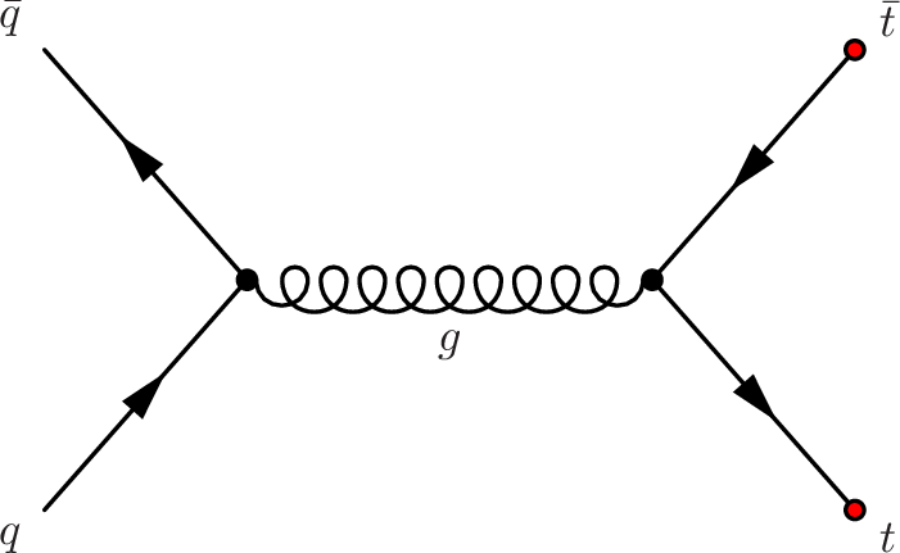
\includegraphics[width=4cm]{fig/f1.png}}
	\subfloat[]{
	\label{Fig.sub.2}
	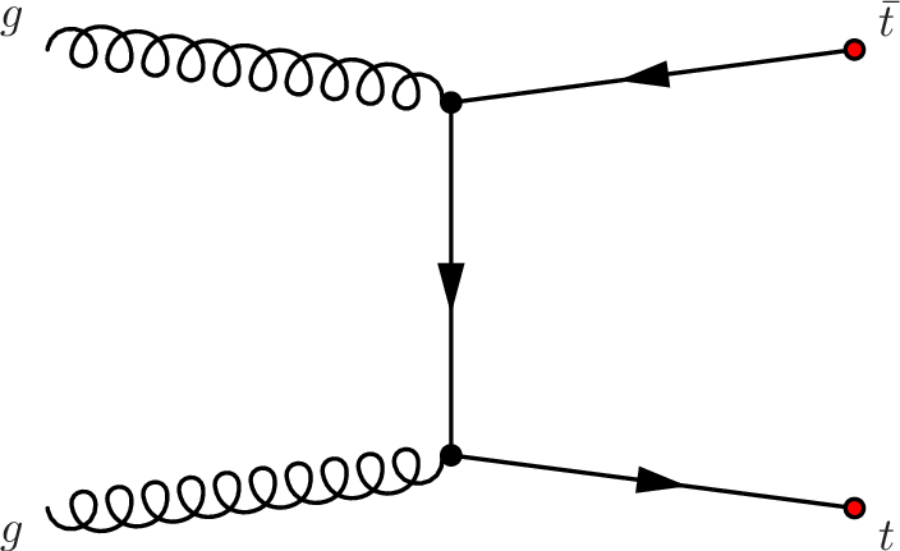
\includegraphics[width=4cm]{fig/f2.png}}
	\subfloat[]{
	\label{Fig.sub.3}
	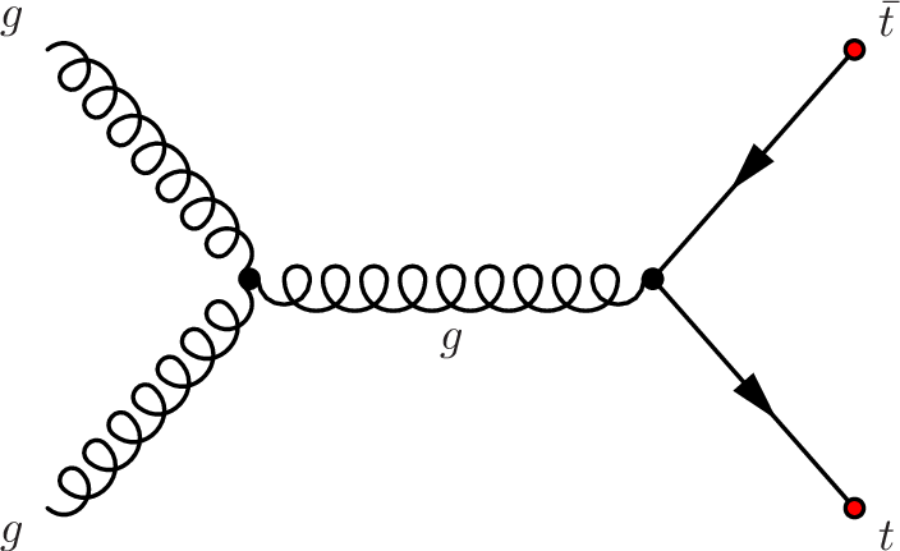
\includegraphics[width=4cm]{fig/f3.png}}
 	\caption[]{Feynman diagrams of strong interaction in top-antitop quarks production via \subref{Fig.sub.1} one gluon exchange in quark-antiquark annihilation, gluon-gluon fusion in \subref{Fig.sub.2} t-channel and \subref{Fig.sub.3} s-channel.}
\end{figure}

With more interactions points involved in, more complicated the calculations become. The effects of self-interactions between particles themselves can happen by producing a virtual particle which is restricted by the uncertainty principle, represented as a loop in a Feynman diagram. The accuracy of the calculation has dependency on the coupling $\alpha_{s}$ and is contributed to a fraction at each order. By including an infinite number of virtual particles, the calculations are led to divergent and infinite.
A set of techniques named renormalization are employed in solving the infinities showed up in the calculations, by which the infinite self-interactions are parameterised by re-scaling them as finite values to compensate the effects. The ultraviolet divergence that occurs from integrating the contributions at extreme high energy is represented by renormalization scale $\mu_R$, on the contrast,  $\mu_F$ represents the condition of an integral diverges at infinitesimal energy.



\subsection{Physics beyond the Standard Model}
\label{sec:2.2}
\subsubsection{$H^\prime$}
%\label{sec:2.2.2}

Many extensions of the SM predict the existence of new heavy Higgs-boson-like particles. 2HDMs are a wide set of models in which the couplings scale with Yukawa couplings thus leads to a relatively small branching ratio of the scale $H$ or pseudoscalar $A$ to gluons~\cite{Harlander:2013qxa}. New particles that decay into photons are also predicted by BSM and have a branching ratio to gluons.  Besides, some classes of models predicted the new particle decaying into photons with a branching ratio to gluons, where the relative branching ratio of photons to gluons is model-dependent. Models with new heavy fermions through scalar decays to gluons are also exist~\cite{PhysRevLett.116.150001,Agashe:2020wph,Curtin:2013fra}.

The motivation of a model-independent di-gluon resonances is that the \mjj background is dominated by valence quark scattering at high energy, which leads gluon tagging particularly effective. At higher energy, there is higher jet constituent multiplicity that makes gluon tagging becomes more effective, thus the search in this analysis could gain the most from gluon tagging.

For this analysis, a high mass simulated $SU(3)$ singlet scalar $H^\prime$ decaying into a pair of gluons is used. The physical width in practice is set to be narrow to be model-dependent and thus the \mjj width is set by the detector resolution.

\subsubsection{String}
%\label{sec:2.2.1}


A mathematical framework named string theory has contributed to a variety of problems in the SM such as the existence of gravity, it offers a unified description of particle physics and gravity. String theory handles point-like particles as one-dimensional objects called strings and demonstrates the behaviours of these strings propagating through time and space. By regarding particles as infinitesimal vibrating strings, the charge, mass, and other properties of them are determined by the vibration or twist of the strings. A dynamical object called brane is employed to generalize the representation of a point particle to higher dimensions such that a string can be regarded as a brane of dimension one and can propagate through time and space under the principles of quantum mechanics. Among them, a so-called Dirichlet membrane (D-brane) is widely used as the open strings satisfy the Dirichlet boundary conditions~\cite{Antoniadis:2000ena,Cremades:2002qm,Antoniadis:2002qm}.

In this analysis, we consider type-II string theory~\cite{StringBook} which includes a D-brane localized in $p$ + 3 partial dimension: D$p$-brane, compactified on a six-dimensional torus. The choice of the string mass scale $M_s$ is to be smaller than the 4-dimensional Planck scale to keep the coupling small, at the expense of introducing 9 - $p$ large transverse dimensions felt only by gravity. Only the fundamental string scale in the TeV range is what this analysis is interested in~\cite{Cullen:2000ef}.


By considering the main subprocesses in dijet production that are independent of the details of the compactification. Amplitudes, which include 2$\to$2 scattering processes involving two gluons and two quarks, or four gluons,  are independent of the details of the compactification such as the configuration of branes~\cite{Lust:2008qc}. This model independence makes it possible to compute the string corrections to QCD dijet processes.


\subsubsection{Quantum Black Holes}
\label{sec:2.2.3}

Quantum Black Holes (QBH), also called micro black holes, are regarded as hypothetical mini (less than a solar mass unit) black holes that dominated by quantum mechanical effects. Some hypotheses predict that QBH could be produced at energies as low as the TeV range, which can be generated in particle accelerators such as the LHC and can be observed through the particles that are emitted by the process of Hawking radiation.


In the simplest scenario, the decay of QBH via Hawking radiation can be approximately described as isotropic decay to a many-particle final state.  The threshold of quantum-gravity energy scale $M_D$ is set to be well below the 
the actual thermal black hole production threshold for gravitational interactions so that two-body states in final states are the dominant, a resonance-like result is expected in predominantly two-body final states as jets near $M_D$. Such isotropic final states is aimed as probes of quantum gravitational effects in this dijet analysis.



%\subsubsection{Graviton}
%\label{sec:2.2.4}
%
%Graviton is at the heart of arguably the biggest challenge in theoretical physics, over decades, physicists have struggled to combine Einstein’s theory of gravity, known as General Relativity, with quantum field theory.
%Graviton is believed to be the carrier of the gravitational field, which means it is the hypothetical elementary particle that mediates the gravitational interactions in the theories of quantum gravity. Graviton is presumed to be massless due to the long range of gravitational interaction and propagates forces and energies at the speed of light as photons.
%There are difficulties in the detection of individual gravitons because of the extremely low cross-section of gravitational interaction with matter. Although gravity affects all particles, its strength at the scale of quarks is predicted to be 10$^{-41}$ relative to electromagnetic force. However, observations such as LIGO and Virgo interferometer have successfully detected cosmic gravitational waves in 2016 and were awarded the Nobel Prize in Physics in 2017.
%Despite the fact that so far no individual graviton has been detected, these experiments still might probe some properties of the graviton. Recent observations of gravitational waves have put an upper bound of  6$\times$10$^{-32}$ eV/c$^2$ on the mass of a graviton.
%
%



\newpage
\fancyhead[C]{The ATLAS Experiment}
\section{The ATLAS Experiment}
\label{sec:3}

\subsection{The Large Hadron Collider}
\label{sec:3.1}

The LHC, built by European Organization for Nuclear Research (CERN) located in Geneva, Switzerland, is the largest circular particle accelerator in the world. The goal of it is to probe the various theoretical predictions made by physicists.
  
It consists superconducting magnets that construct a 27-kilometer ring lying in the tunnel under the ground. Inside the LHC, two beams made of protons or ions are accelerated to extreme high speed in opposite direction in individual vacuum pipes then made into collision by a strong magnetic field within the structures.

The LHC is the last section of the CERN accelerator complex where a series of machines accelerates the particles to increasingly higher and higher energies. The highest energies of beams are reached at the LHC.


 \begin{figure}[htb] 
 	\centering  
 		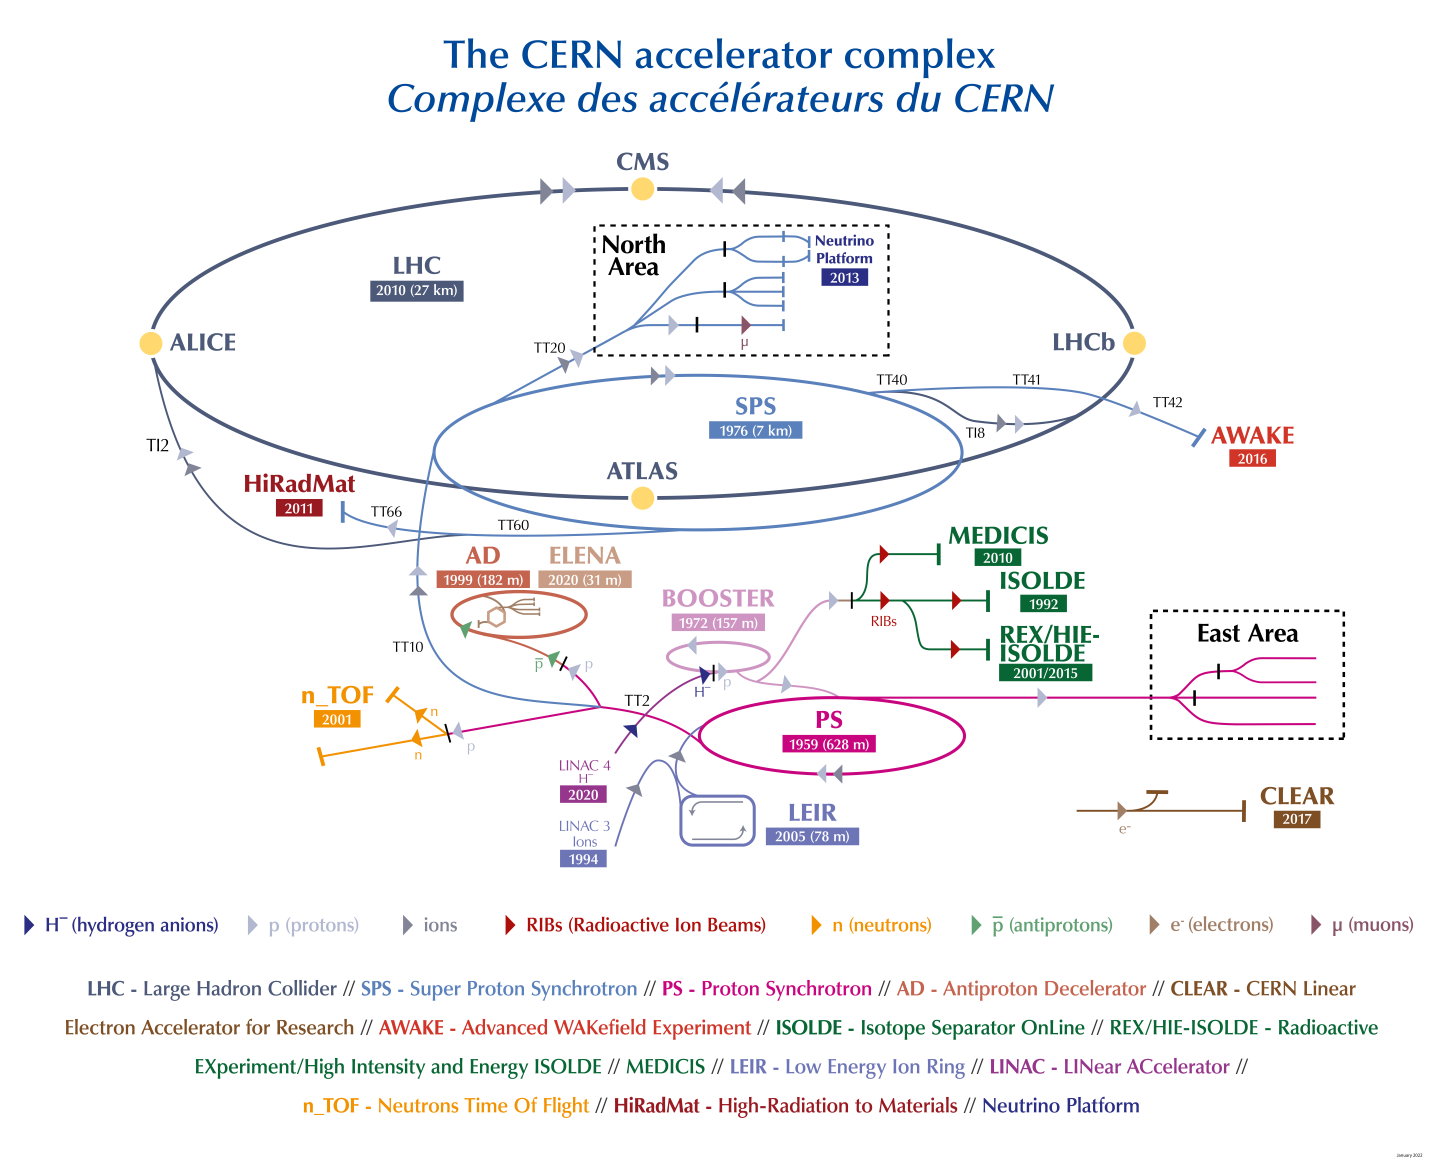
\includegraphics[width=14cm]{./fig/2022.png}
 		\caption{The CERN accelerator complex}
\end{figure}
 

 Seven detectors are placed around four collision points in the collider. Different types of particles are accelerated according to the research, the main beams are protons, but the LHC also run beams of heavy ions as lead–lead collision or proton-lead collisions.
 
 The energy of particles is increased by a series of processes before being injected into the main accelerator. For a proton-proton collision, negative hydrogen ions are generated by the linear particle accelerator Linac4 at 160 MeV then injected into the Proton Synchrotron Booster, where protons are obtained by stripping electrons away from the atom and accelerated to 2 GeV. After entered the Proton Synchrotron the energy of the protons is 26 GeV, and then their energies are increased in Super Proton Synchrotron to 450 GeV before they are finally injected into the main ring. 

  
One of the characteristics that defines the power of an accelerator is the centre-of-mass energy, which represents the total momentum of the system and thus indicates the total mass of potential new particles as well as probes the internal structure of known particles under the law of energy invariant within the system. In 2010, the first collisions were made at an energy of 3.5 TeV each beam, later in 2018, an energy of 6.5 TeV per beam was achieved, resulted in the centre-of-mass energy of 13 TeV where the protons moved at a 99.9\% speed of light. It took less than 90 $\mu$s for photons to go through the whole LHC ring. 

Other quantities such as luminosity, denoted as $\mathcal{L}$, also represents the performance of an accelerator. It is the rate of interactions during a certain period of time and can be expressed as:

\begin{equation}
\mathcal{L}=\frac{N^2 f_{r e v}}{4 \pi \sigma_x \sigma_y} 
\end{equation}
where $N$ is the number of particles in a bunch, in the case that a beam has Gaussian distribution and has brunches crossing frecuency $f_{rev}$. $\sigma_x$ and $\sigma_y$ denote as transverse beam widths in the x- and y-plane. The luminosity takes the units of cm$^{-2}$·s$^{-1}$.

The total number of physics events detected can be express as:

\begin{equation}
N_{\text {event }}=\sigma_{\text {event }} \cdot \int \mathcal{L} d t \equiv \sigma_{\text {event }} \cdot L
\end{equation}

where $L$ is the integrated luminosity with respect to time, $\sigma_{\text {event }}$ is referred to the cross section of a specific physics process. The integrated luminosity takes the units of cm$^{-2}$ which equals to the unit femtobarn (fb).

 At the LHC, thousands of magnets around the accelerator are operated at a very low temperature of ‑271.3\textcelsius \ to maintain its superconducting state which allow them to conduct electricity without loss of energy. Hence, a system of liquid helium is used for cooling the accelerator and supply services.

Besides, superconducting radio frequency cavities which resonate electromagnetic fields are employed to accelerate the protons. Instead of having continuous beams, the protons are made into bunches, so that the collisions are taken place at discrete intervals between two beams with 115 billion protons per bunch at the frequency of 25 ns.


\subsection{The ATLAS detector}
\label{sec:3.2}

The ATLAS detector~\cite{PERF-2007-01} is the largest volume detector ever constructed for general-purpose particle research at the LHC. It has the shape of a cylinder with 44 meters long, 7000 tonnes in weight and 25 meters in diameter, sitting in a cavern underground. It is designed to collect evidence of the properties of SM and search for new predictions made by particle physics beyond the SM.

To record the energy, momentum and trajectory of particles after collisions, the detector consisting of 6 different detecting subsystems  placed in layers surrounding the interaction point to measure them individually and effectively. 

 \begin{figure}[htb] 
	\centering  
	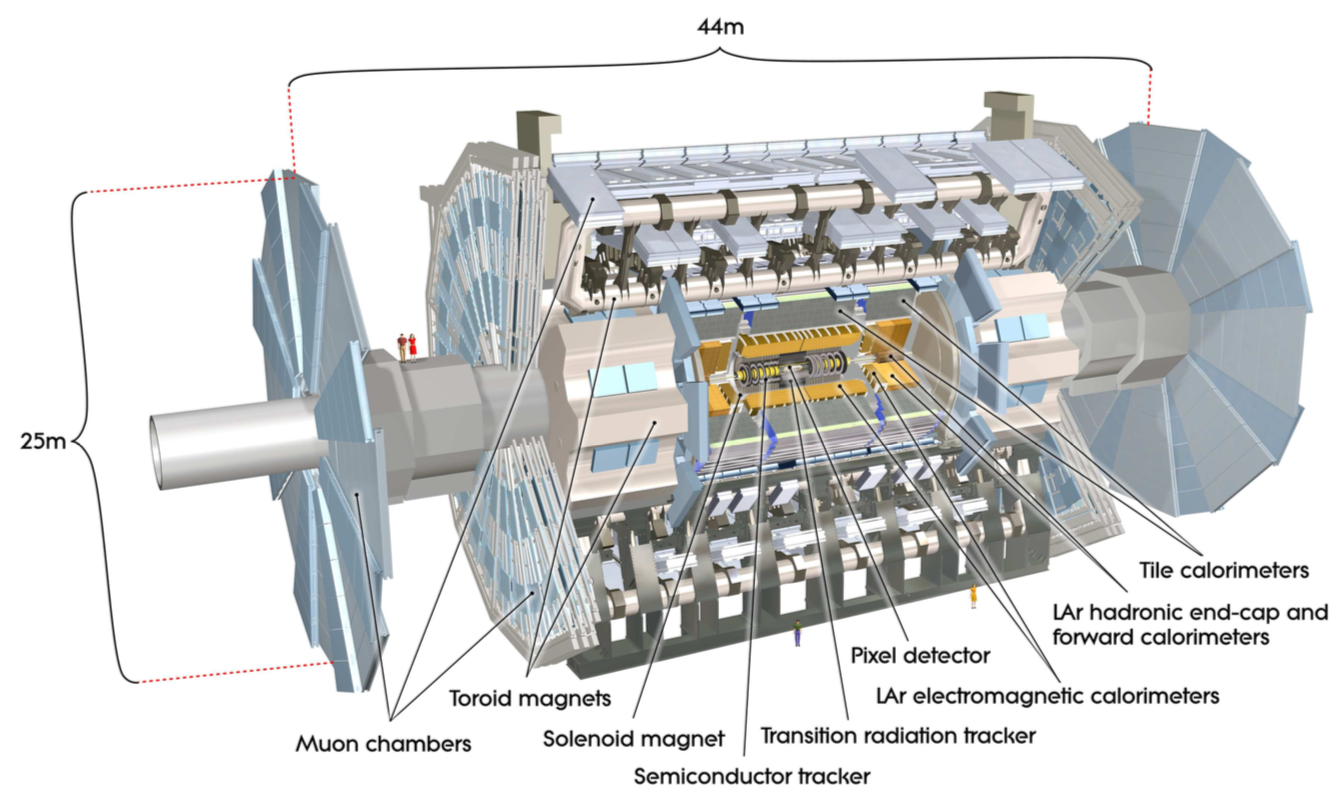
\includegraphics[width=14cm]{./fig/atlas.png}
	\caption{Cut-away view of the ATLAS detector}
	\label{Fig.atlas}
\end{figure}
An overall layout of the ATLAS detector is shown in Figure~\ref{Fig.atlas}.

\subsubsection{Inner detector}
\label{sec:3.2.1}

Charged particles above a certain \pt~threshold are detected by the ATLAS Inner Detector (ID) which immersed in a 2 T solenoidal field, covered the pseudorapidity range \abseta < 2.5.
Appearing as tracks in the ID, an excellent momentum resolution as well as both primary and secondary vertex of them are provided by the ID.  Within the range \abseta < 2.0,  electron identification is also provided.

The layout of the ID is shown in Figure~\ref{Fig.id} in cylindrical coordinate: $r=\sqrt{x^2+y^2}$, where $x$-axis alongside the LHC ring and $y$-axis is perpendicular to the $x$-axis.
\begin{figure}[htb] 
	\centering  
	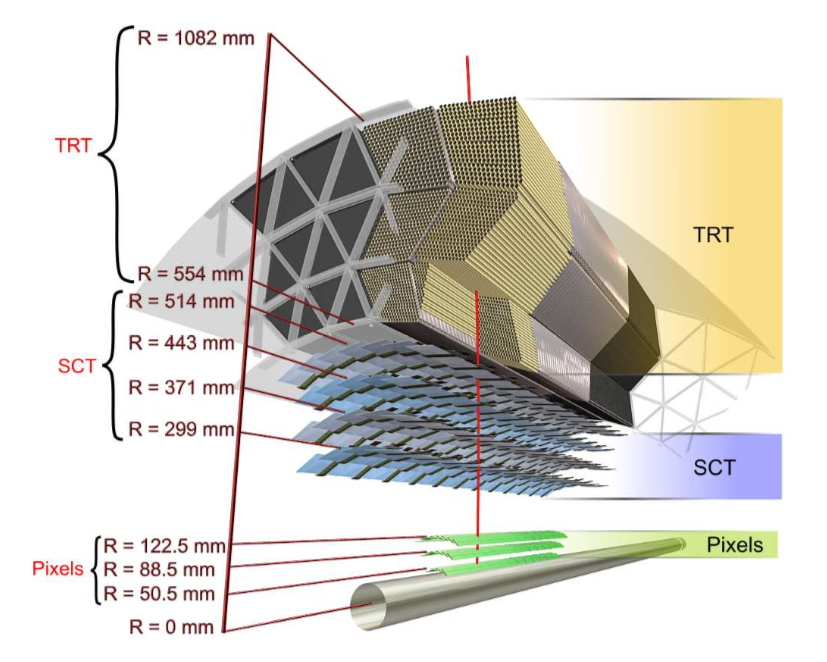
\includegraphics[width=13cm]{./fig/id.png}	\caption{Cut-away view of the ATLAS ID. Sensors and structural elements traversed by a charged track of 10 GeV \pt~in the barrel inner detector along with their envelopes in $r$.}
	\label{Fig.id}
\end{figure}

A cylindrical container around the ID has a length of 3512 mm each way and a radius of 1150 mm, tracks of 10 GeV traverse the sensors and structural elements in the barrel and end-cap regions, respectively.

Within the inner region, a series of discrete space points provided by the silicon pixel detector and stereo pairs of silicon microstrip semiconductor tracking (SCT) layers gives high-resolution pattern recognition abilities. By increasing radial distances, the transition radiation tracker (TRT) provides extra pattern recognition and momentum resolution capabilities.

\begin{description}
 \item[The pixel detector] \mbox{} \\
A series of high-granularity measurements is provided by the pixel detector~\cite{PIX-2018-001} which is composed of the innermost sub-detector of the ID, it is designed as close to the interaction point as possible. Three sub-sections: two end-cap perpendicular to the beam axis and a barrel alongside the beam axis as a concentric cylinder with four layers (average radii of 33.25, 50.5, 88.5 and 122.5 mm, respectively) in it. 

The innermost pixel layer (or B-layer, IBL) is essential to b-tagging performance and supersymmetry searches as it cover the full acceptance of short-lived particles such as B hadrons and $\tau$ leptons from the beginning of Run-2 to enhance the measurement of the secondary vertex. Besides, a new readout sensor and chip responsible for higher radiation demage and higher hit rate, respectively, is employed in the IBL compared to the other three layers in the barrel region. A new  n-in-n planar and 3D silicon sensors with hit efficiency of greater than 97\% is developed as well. The better impact parameter resolution is achieved by reducing the pixel size of the chip down to 50 $\times$ 250 $\mu$m$^2$.  Around 80 million readout sections counting them all provide the great  hit resolution of 10 $\mu$m in radius plane and 115 $\mu$m alongside the z-axis in the pixel detector.

 \item[The semiconductor tracker] \mbox{} \\
 Surrounding the pixel detector is the SCT which encompasses silicon based semiconductor sensing components in barrel and end-cap geometries. Four silicon microstrip layers, located at radii of 300, 373, 447 and 520 mm, in the barrel region of the SCT provide high granularity points. The mean size of each strip pitch is 80 $\mu$m for the rectangular barrel sensors as daisy-chained with 6 cm-long. For the end-cap sensors, nine disks cover \abseta  < 2.5 are chosen. As a results, there are thus 768 readout strips with 6.36 $\times$ 6.40  cm$^2$ in size in total, with additional two strips at the edge of the sensor. 6.1 m$^2$ of silicon detectors with 6.2 million readout channels as a whole intergrated the SCT. 
 
 \item[The transition radiation tracker] \mbox{} \\
 The outermost layer of the ID is the TRT which encompasses polyimide drift(straw) tubes that designed to enable as much less wall thickness and material as possible while maintaining the good experimental properties. With 4 mm in diameter and 150 cm in length, 73 layers of 144 cm alongside the beam with 50 thousands tubes and 37 cm tubes consisting 160 tubes planes in the end-cap with 320 thousands radial tubes.
 
 The xenon-based gas filled up in a given tube provides the track hit of a particle as it ionized as the emitting electrons drifting to the center wire of the tube volume. An average of 36 hits per charged-particle track is given by the TRT, 
 The resulting electrical signals are obtained by converting the drifting charge currents. In total 420 thousands of electronics channels in which a good spatial resolution and drift-time measurement are provided by the TRT, enhancing the precision measurements of momentum in the ID.  
 

\end{description}

\subsubsection{Calorimeters}
\label{sec:3.2.2}

Outside of the ID lies the ATLAS calorimeters system which is designed to obtain the energy lost of the particles that travel through the detector components. Multiple layers of high-density material are placed to consume the energy of the incoming particles inside the materials and stop them from further moving.  An “active” medium is left inside the layers that allows experimental physicists measure the energy of those particles.

Two types of calorimeters are employed in the ATLAS calorimeters system: the energy of electrons and photons are measured by the electromagnetic calorimeters as they create reaction with matter. Hadronic showers that created by the interaction between hadrons and atomic nuclei, are sampled by the hadronic calorimeters. Muons and neutrinos can not be stopped by the calorimeters as they interact only weak force but the track footprints could be seem in the calorimeters. The layout of the calorimeters is shown in Figure~\ref{Fig.calo1}.

\begin{figure}[htb] 
	\centering  
	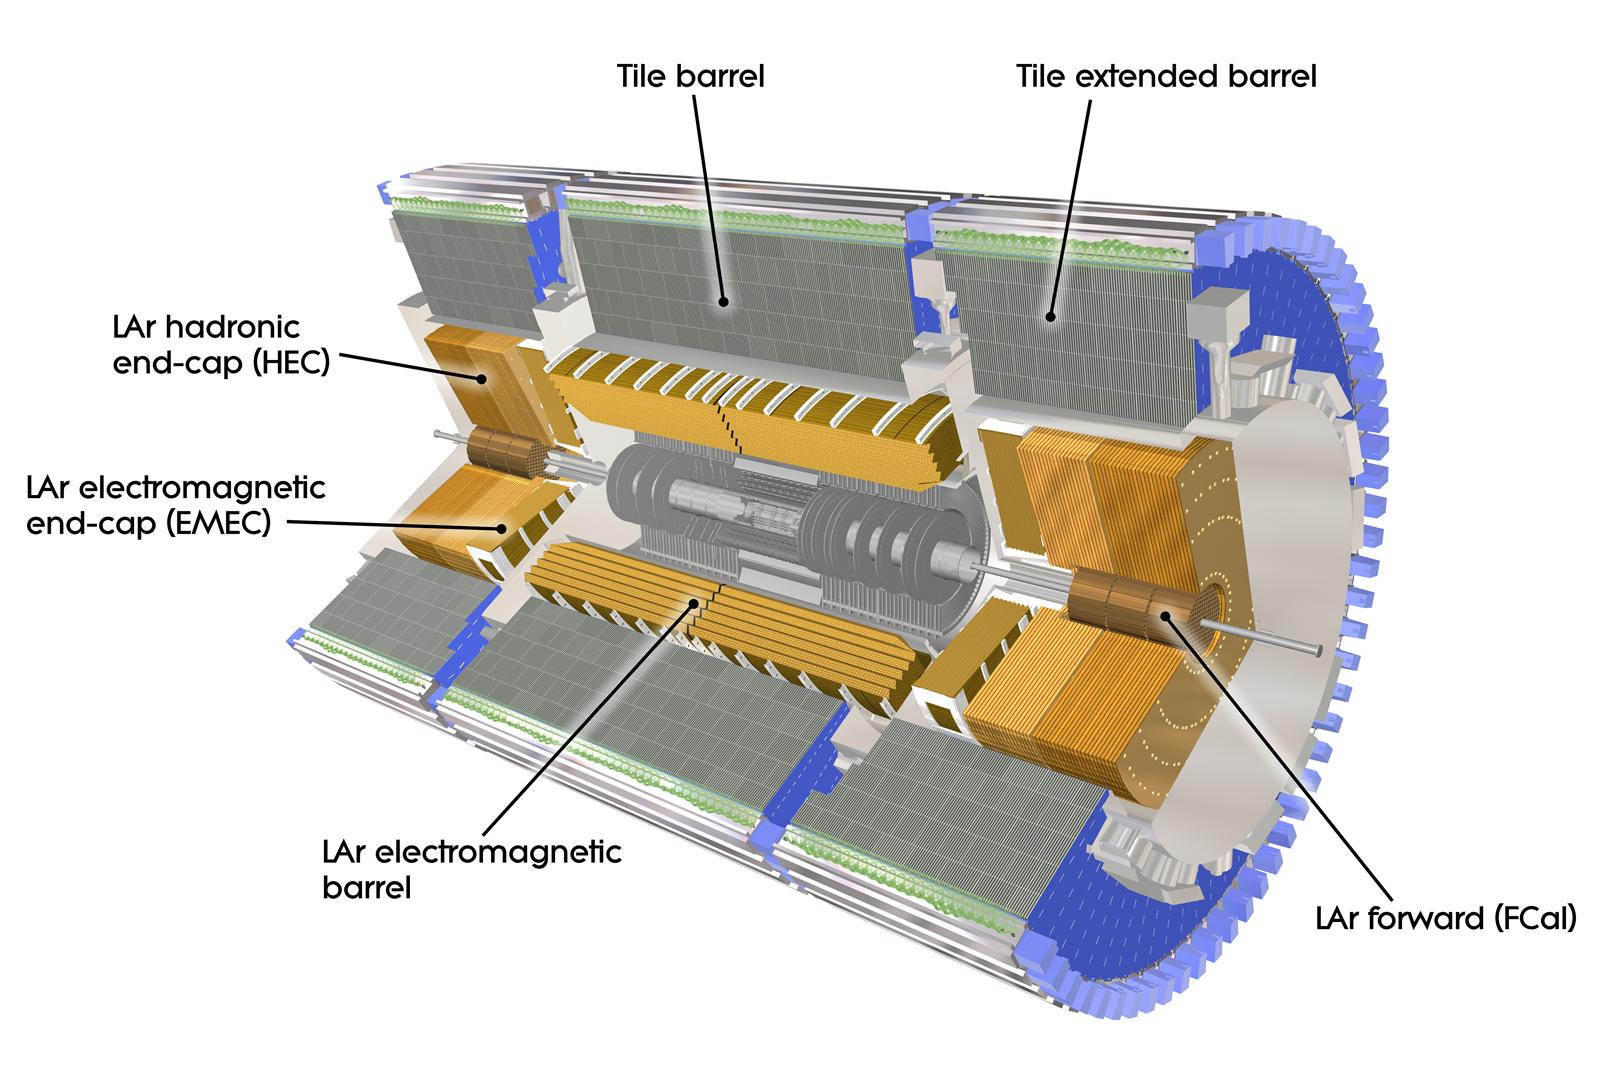
\includegraphics[width=15cm]{./fig/calo1.jpg}	\caption{Outline of the ATLAS Run 2 trigger and data-acquisition system.}
	\label{Fig.calo1}
\end{figure}

The electromagnetic (EM) calorimeter covers a range of  \abseta < 3.2 by combining the one barrel and two end-cap modules as cylindrical cryostat, with an outer radius of 2.25 m, an end-cap thickness of 0.632 m and a length of 3.17 m. The hadronic calorimeter covers the central barrel region of \abseta < 1.0 and two extended barrels in a region of 0.8 < \abseta < 1.7. with a radius of 2.28 m at the inside and 4.25 m at the outside. Figure~\ref{Fig.calo2} demonstrates the positions of the end-cap of the calorimeters including the EM and Hadronic calorimeters.



\begin{figure}[htb] 
	\centering  
	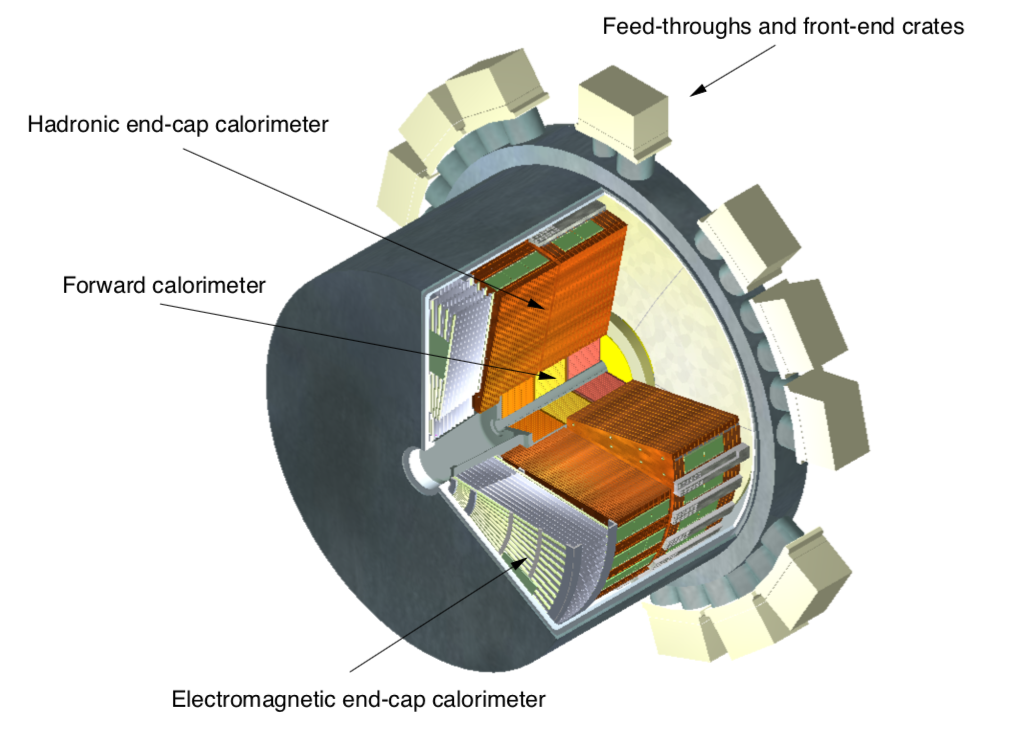
\includegraphics[width=15cm]{./fig/calo2.png}	\caption{Cut-away view of an end-cap cryostat of the ATLAS calorimeter system.}
	\label{Fig.calo2}
\end{figure}



\begin{description}
	\item[The electromagnetic calorimeter] \mbox{} \\
The EM calorimeter that surrounding the ATLAS ID is designed for the high-granularity measurements of the energy of photons, electrons and hadrons with Liquid Argon (LAr) sandwiched between the multiple layers ionised. It converts the incoming particles into electric currents by absorbing the energy of these particles as they interact with the metal with the bremsstrahlung phenomenon. A pair of electron-positron produced by an electron radiation in the EM calorimeter can initiate further electron-positron pairs (as showers) until the energy of the particles fall below the certain threshold, the dominate process thus become ionisation in the LAr where drifting electrons are produced. Furthermore, the missing transverse energy can be obtained by subtracting the total energy of the known particles, which contributes to the analysis of neutrinos and new particles.

At -184 \textcelsius~where the argon exists in liquid form, the calorimeter is kept as the cables that transverse electronic signals are sealed in vacuum and connected to the warmer area where located the readout system.




\item[The hadronic calorimeter] \mbox{} \\
Surrounded the EM calorimeter, lies the tile hadronic calorimeter where hadrons that contain strong force thus could not fully deposit their relatively large energy in the EM calorimeter are absorbed by the tile calorimeter. Steel and plastic scintillating tiles are placed in layers in order to record the trajectories of incoming particles as hadronic showers are formed by the interactions of the particles with the materials and emitting particles continue interacting with materials in the hadronic calorimeter and more particles are produced in steel layers. On the other hand, photons are produced by the plastic scintillators where electric currents are gained according to the energy of the particle.

By enveloping the EM calorimeter, a hadronic shower that contained EM showers can be fully absorbed by the great thickness in the hadronic calorimeter. Around 420 thousands of plastic scintillator tiles are placed in sync, leading a weight of 2.9 thousands tonne in total.

\begin{figure}[htb] 
	\centering  
	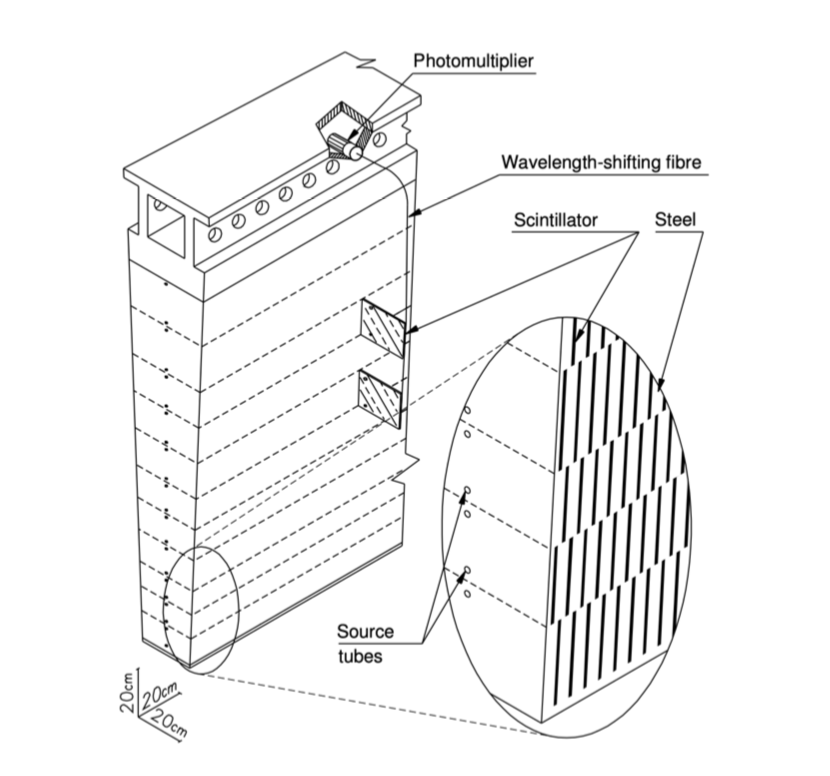
\includegraphics[width=11cm]{./fig/tile11.png}	\caption{A schematic view of a tile calorimeter components of optical readout tiles and scintillating tiles.}
	\label{Fig.Tile1}
\end{figure}

As illustrated in Figure~\ref{Fig.Tile1},  photomultiplier tubes (PMT) are placed around the outer radii of the tile calorimeter and connected with wavelength-shifting fibres by which scintillation light is transferred. Projective geometry is designed for the whole readout system as the energy of most hadronic showers is deposited in the first or last two layers.  Though the coarser granularity of the readout cells of hadronic calorimeter has been compared to the EM calorimeter, the hadronic calorimeter is qualified for the measurement of transverse momentum and jet reconstruction.

In the forward regions, the hadronic calorimeters are integrated with LAr calorimeters due to higher radiation exposition compared to the barrel regions. There are two calorimeters that were developed to tackle such issue: the hadronic end-cap calorimeter (HEC) that covers 1.5 < \abseta < 3.2 and the forward calorimeter (FCal) that covers 3.1 < \abseta < 4.9.

The HEC located further beside the EM end-cap calorimeter has two wheels in each end-cap.  LAr is used for filling up 8.5 mm between copper layers in the HEC, by which the active medium is provided. The readout electrodes are provided in separate drift zones in order to secure the stability of the whole system.  The FCal has three wheels placed alongside the z-direction: one electromagnetic layer (FCal 1) and two hadronic layers (FCal 2 and FCal 3). LAr is also used as an active medium in all of the layers. As for the absorber, copper is employed in FCal 1 as it has heat removal properties.  Tungsten is used in both FCal 2 and FCal 3 in order to constrain the lateral spread of hadronic showers. 
\end{description}


\subsubsection{Muon spectrometer}
\label{sec:3.2.3}

The muon spectrometer (MS), specially designed for the muon detection is located in the outermost section of the ATLAS in order to provide sufficient measurement of high-momentum muons which are almost "invisible" to the ID and calorimeters due to little energy deposit when traveled through the them. By deflecting the trajectories of muons, the MS employs the magnetic field by a barrel toroid magnet system in \abseta < 1.4 and end-cap toriod systems in 1.6 < \abseta < 2.7. 

Four subsections of the MS: add up to 4000 separate muon chambers. Thin Gap Chambers (TGC) and Resistive Plate Chambers (RPC) account for triggering and the second coordinate measurement of muons. TGC is set at the end of the detector whereas RPC which provides 5,000 V/mm electric field is placed in the central region. Monitored Drift Tubes (MDT) is designed for the curve of muon tracks measurement with fine tube resolution of 80 $\mu$m. Cathode Strip Chambers (CSC) accounts for measuring coordinates precisely located at ends of detector with a fine resolution of 60 $\mu$m. Figure~\ref{Fig.ms} demonstrates the MS with all four subsections. In total three separate points within the muon trajectory are measured to reconstruct the momentum of the muon.


\begin{figure}[htb] 
	\centering  
	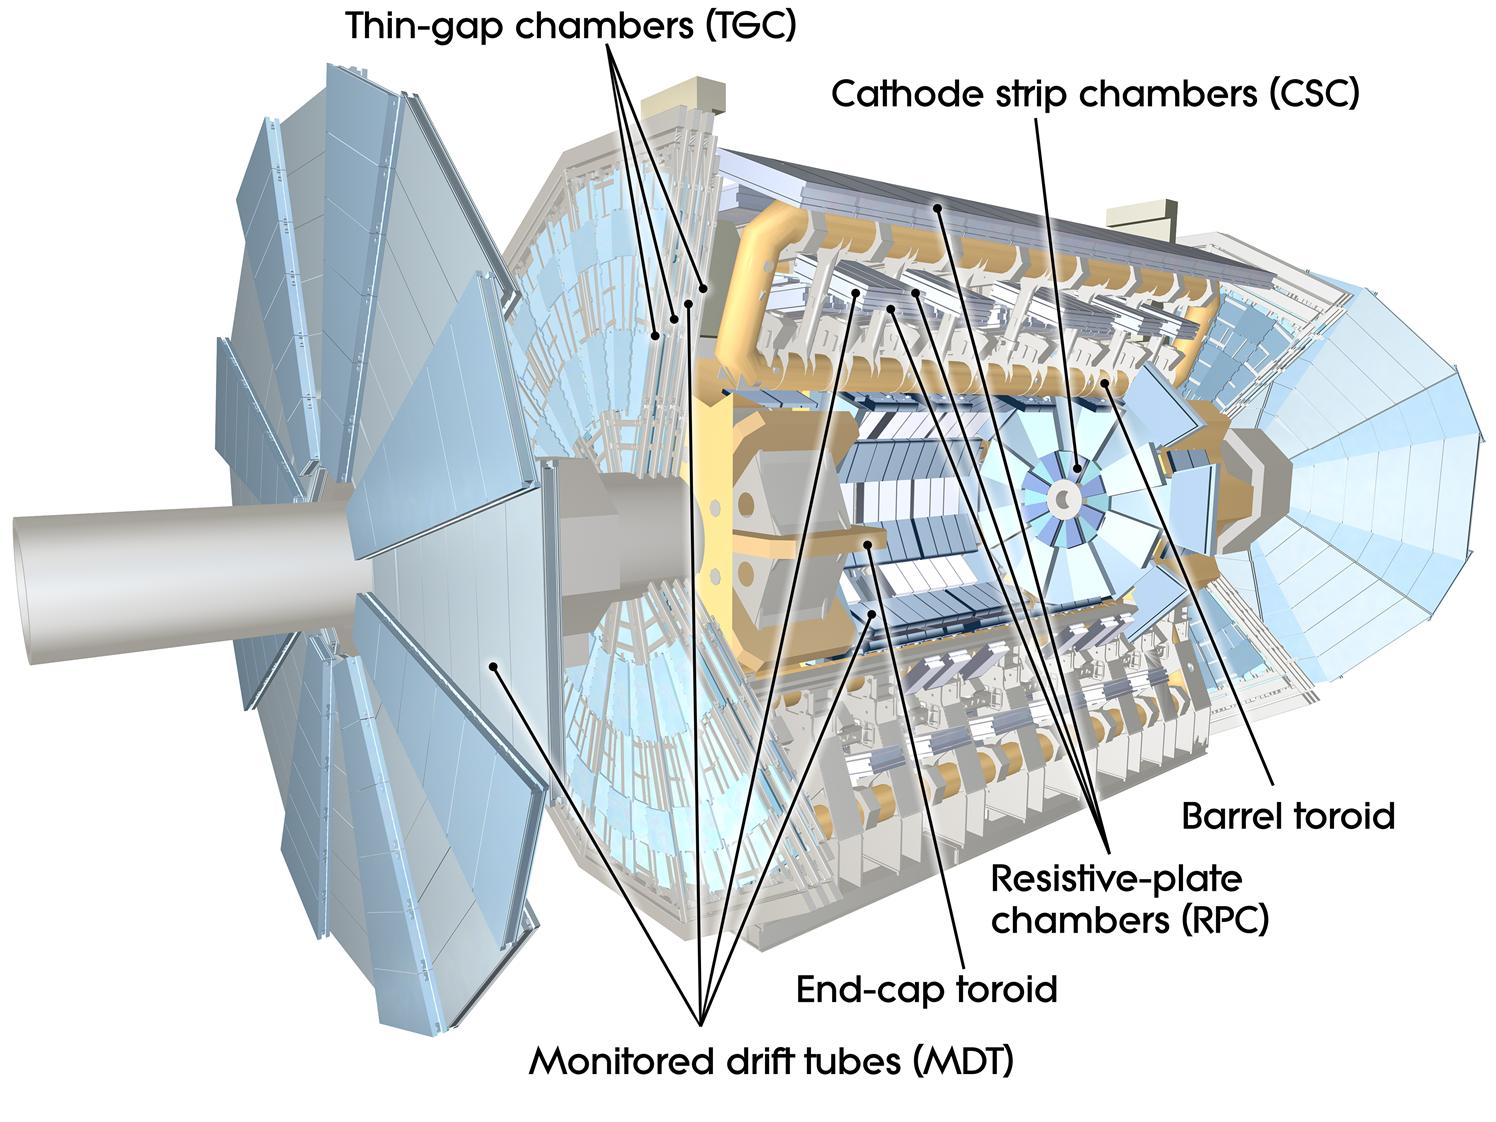
\includegraphics[width=14cm]{./fig/muon.jpg}	\caption{Cut-away view of the ATLAS Muons Spectrometer with subsections labeled.}
	\label{Fig.ms}
\end{figure}

\subsubsection{Trigger and data acquisition}
\label{sec:3.2.4}

At the LHC, approximately 1.7 billion proton-proton collisions occur per second at an integrated luminosity of 140 \ifb. However, many of these collisions are unlikely to produce characteristics of interest. As a result, large numbers of events can be discarded without affecting the search for new physics. The trigger and data acquisition systems are introduced to eliminate the irrelevant data so that only events of suitable quality and quantity are recorded.

\begin{figure}[htb] 
	\centering  
	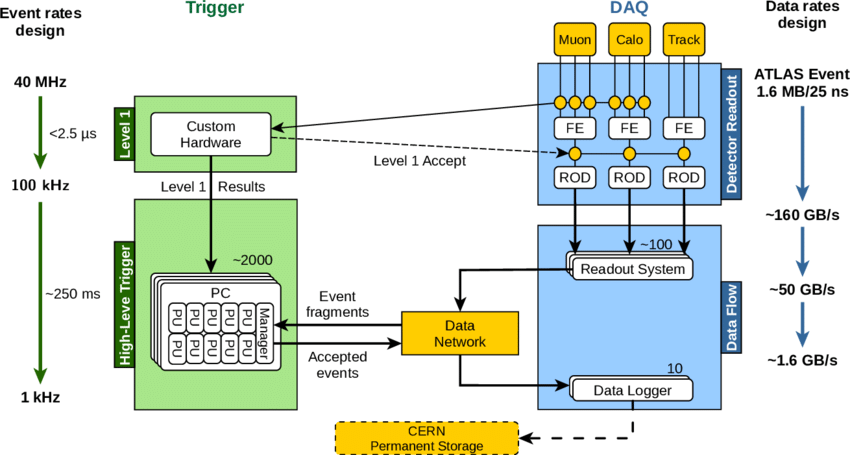
\includegraphics[width=16cm]{./fig/dq.png}	\caption{illustration of the ATLAS  Run 2 trigger and data acquisition system.}
	\label{Fig.dq}
\end{figure}

During the year of 2015-2018, the trigger system in ATLAS selected significant events in a two staged process, as illustrated in Figure~\ref{Fig.dq}: The first-level (L1) trigger is implemented on hardware, and reduced event rates from 40 MHz to 100 kHz in less than 2.5 $\mu$s right after the data happened. Working with the electrical information provided by the calorimeters and the MS, the L1 trigger employs custom-made electronics to filter and store the events in the readout sections as buffers before passing them to the High-Level trigger (HLT)~\cite{TRIG-2016-01}. Certain physics objects such as photons, jets and leptons are identified in the L1 trigger, in which energy depositions of electrons and photons in the EM calorimeter and jets in the hadronic calorimeter are provided. Information of tracks in high-momentum muons is recorded in the layers of the MS and forwarded to the L1 trigger.

The events are further reduced from 100 kHz to 1 kHz in merely 250 microseconds by the second level trigger: HLT. Based on the offline software, the HLT utilize fast selection algorithms to analyse and reject events in the early stage, resulting in better precision and intense CPU usage of about 1.6 GB per second.  The accepted data from the HLT will be passed to permanent storage at CERN via Data Logger~\cite{ATL-SOFT-PUB-2021-001}. 



\newpage
\fancyhead[C]{Jets in ATLAS}
\section{Jets in ATLAS}
\label{sec:4}


In the LHC, a large number of quarks and gluons are produced during the inelastic proton-proton collisions, resulting in jets. These collimated outcome particles are hadronised because of colour confinement in the QCD process. As a result of this, only colour-neutral jets clustered by particles can be seen in the detector.

The information of jets is crucial to most of the analysis such as the measurements of the SM particles and searches for the BSM phenomena. Good qualities of jets, for example the high efficiency of jet reconstruction, jet energy calibration including energy scale and energy resolution, are thus important to the analysis.

\subsection{Jet reconstruction}
\label{sec:4.1}

Jets are defined in two way:  Monte Carlo (MC) simulated jets at particle level and detector level jets with the information from the ID and calorimeters. The production and hadronisation processes of jets are illustrated in Figure~\ref{Fig.jet}.

\begin{figure}[htb] 
	\centering  
	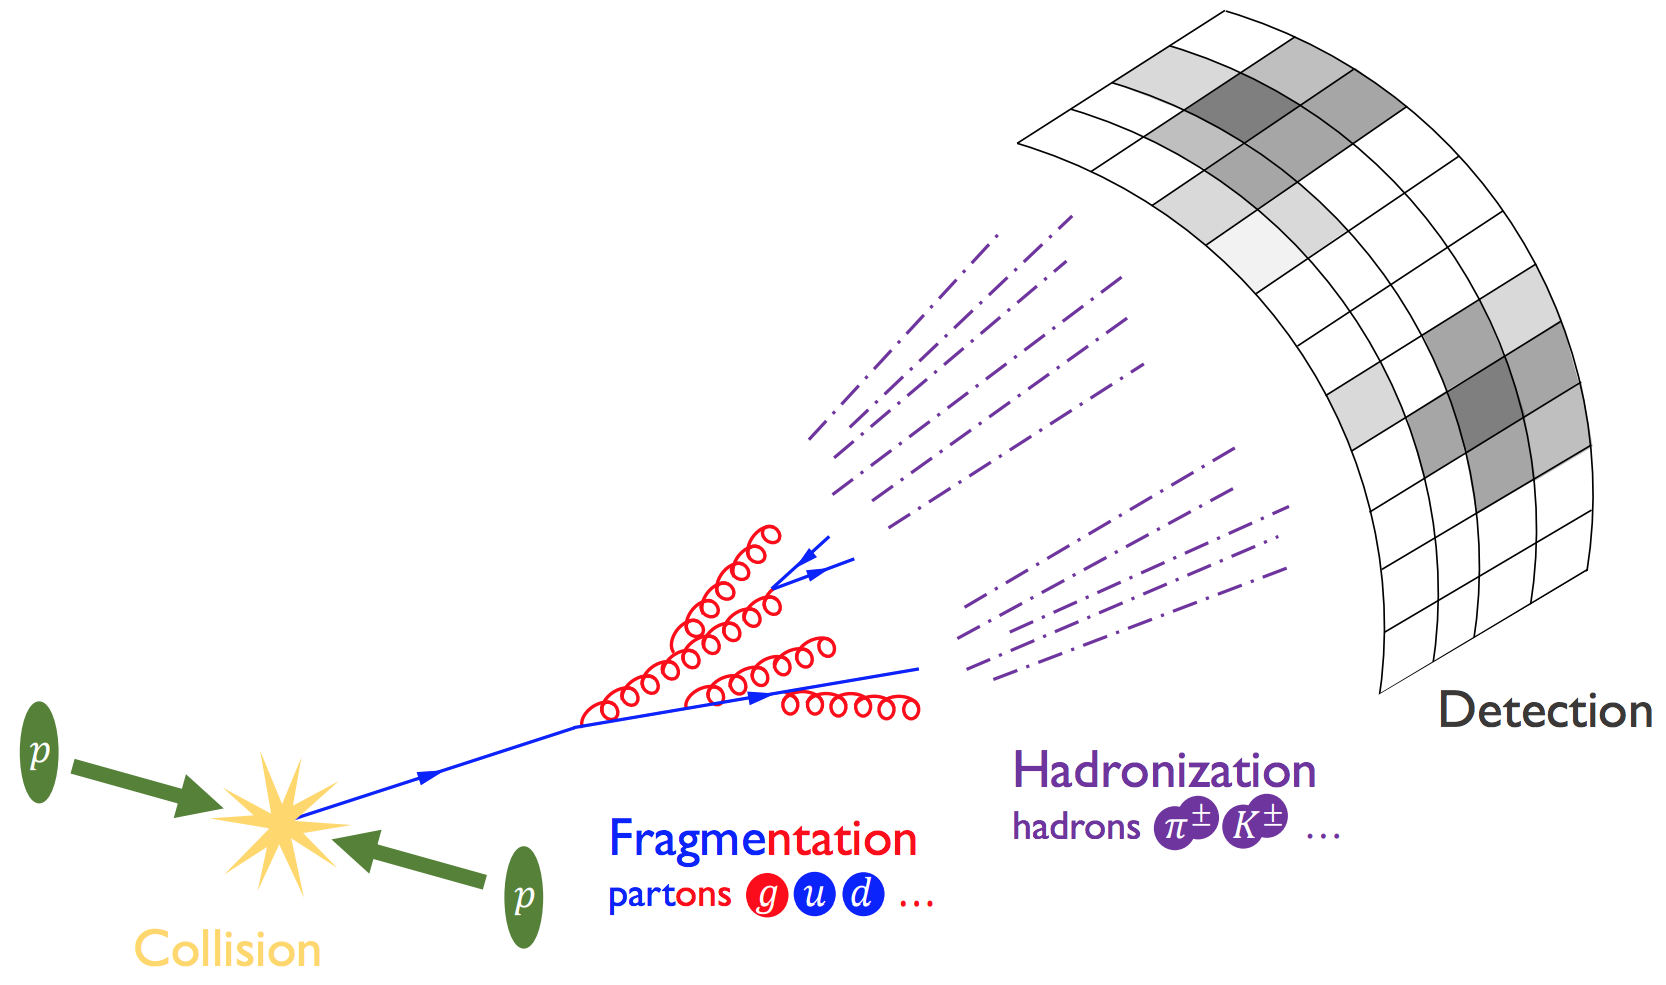
\includegraphics[width=15cm]{./fig/jet.jpg}	\caption{illustration of jets produced by pp collision and hadronised before seen by the detector.}
	\label{Fig.jet}
\end{figure}

Jets from the MC simulation are defined as truth-particle jets which have lifetimes longer than 10 ps as stable particles. Truth-particles indicate the ideal measurement from a detector under perfect-condition and high resolution without defects or the effects from pile-up (background interactions per bunch-crossing in the LHC). Whereas track jets are constructed with the use of charged information in the ID, and calorimeter jets with the use of energy information in the calorimeters.

There are several types of jets aim for different analysis depended on the constituents and algorithm used for reconstructing the jets. ATLAS previously used topo-cluster jets, which is a group of topological related cells in calorimeter with significantly high energy deposits. A pile-up suppressed algorithm is applied to select certain cells with low noise. Cell above certain signal-to-noise (S/N) threshold (usually by four times its standard deviation) are used to seed the algorithm. By neighbouring the seed a topo-cluster is defined. In the hard-scatter process, jets of interest are expected to produced from the primary interaction point (known as vertex). The primary vertex is defined if there are at least two tracks with the highest sum of squared track momentum associated to it.

Jets are constructed from any set of four-vectors. EMTopo jets are the jets that use topo-cluster initially calibrated to electromagnetic (EM) scale in the calorimeters. A local cluster weighting (LCW) scale is also used for calibrating hadronic clusters by applying weights for low hadronic interaction response. Besides, particle flow (PFlow) jets are built by combining the information from both the ID and the calorimeter, where the energy deposited from the calorimeter are removed by the momentum in the ID by a cell-based energy subtraction algorithm. The inputs to the particle flow algorithm are the separate topo-clusters with local energy maxima, respectively. 

A recombination algorithm called anti-$k_t$ algorithm is employed to build the jets with a radius parameter $R$ in rapidity-azimuth $(y-\phi)$ plane around a cluster. The algorithms are defined as follows:

\begin{equation}
d_{i j}=\min \left(k_{\mathrm{t} i}^{2 p}, k_{\mathrm{t} j}^{2 p}\right) \frac{\Delta_{i j}^2}{R^2}
\end{equation}

\begin{equation}
\Delta_{i j}^2=\left(y_i-y_j\right)^2+\left(\phi_i-\phi_j\right)^2
\end{equation}

\begin{equation}
d_{i B}=k_{\mathrm{t} i}^{2 p}
\end{equation}
where the distance $d_{i j}$ between any pair of particles $i$ and $j$ is given by the minimum transverse momenta $k_t$ of the two particles. The geometrical distance $\Delta_{i j}$ represents the separation of a pair of particles in $(y-\phi)$ plane. Radius parameter $R$ indicates the size of the final jets. The distance $d_{i B}$ between any detected particle i and the beam $B$ is also given. Parameter $p$ indicates the relative power of of energy with respect to geometrical scales and is used to distinguish the different types of algorithms.

When $p$ is set to 0,  the Cambridge-Aachen (CA) algorithm is given as the distance $d_{i j}$ and $d_{i B}$ only based on spatial separation and are independent of the transverse momenta. This algorithm is usually used for large-radius jets and jet substructure performance study.

For the $k_t$ algorithm, $p$ is set to 1 so that the distance $d_{i j}$ is dominated by the minimum $k_t$. This algorithm is preferred for clusters that are soft and collinear splits are merged first, resulted in irregular footprint with the most interesting splits.

The  \antikt~algorithm on the other hand set $p$ = -1, leaving the distance $d_{i j} \propto \min \left(\frac{1}{k_{t i}^2}, \frac{1}{k_{t j}^2}\right)$ shorten as the transverse momenta of two particles increase. This is widely used in the LHC for hard clustering as it is less vulnerable to the effects from the pile-up and resulted in circular footprint as shown in Figure~\ref{Fig.kt} for $R = 1.0$.

\begin{figure}[htb] 
	\centering  
	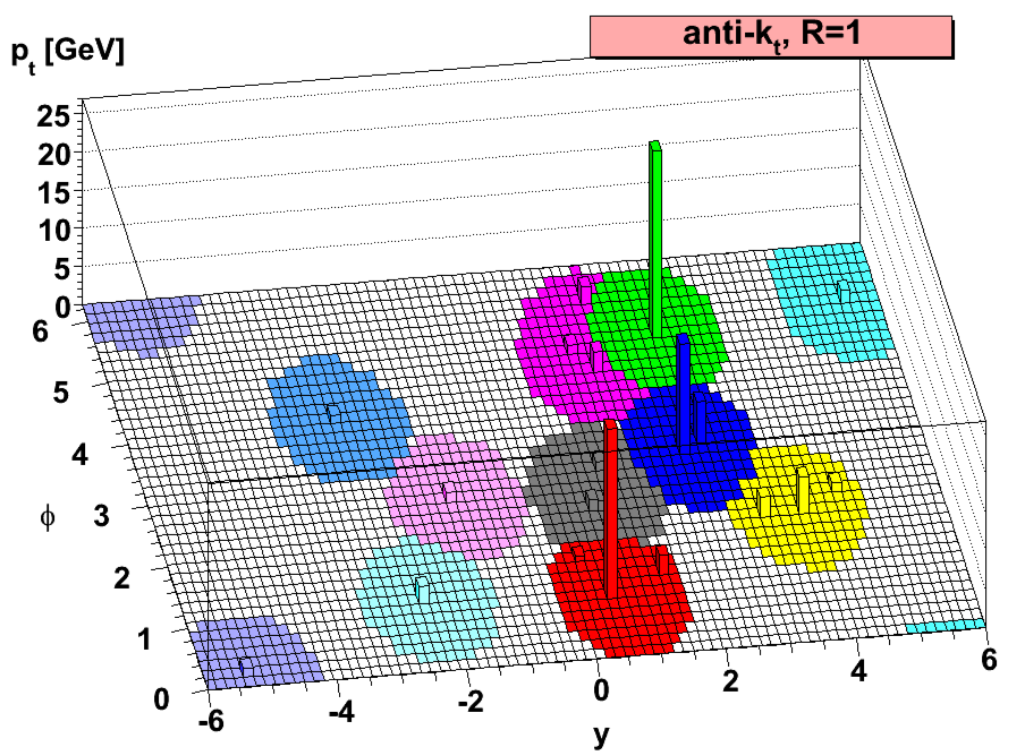
\includegraphics[width=12cm]{./fig/kt.png}	\caption{Plot of parton-level jets clustered using  \antikt~algorithms with radius parameter set to 1.}
	\label{Fig.kt}
\end{figure}

For most of ATLAS analysis, jets with $R = 0.4$ are used for quarks and gluons analysis. Other ones such as $R = 1.0$ are also widely used to study energetic particles like W and Z bosons. $R$ = 0.2, 0.6, 1.2, 1.5 and variable radii are also analysed.

The \antikt~$R = 0.4$ PLow jets are used in the quark/gluon taggers calibration described in this thesis.



\subsection{Jet calibration and cleaning}
\label{sec:4.2}

The motivation of jet calibration is to correct the translation from received signals to initial partons for several detector effects, including energy deposited in dead or beyond areas in the detectors, low response to hadronic reactions, pile-up, radiations that outside jet cone, etc. The calibration process is thus needed to account for the energy of jets to that of MC simulated jets at particle-level.

Calibration is performed to topological clusters at the EM scale where the sum of the energies in all constituent cell are taken, or at the LCW scale where low hadronic response in the ATLAS calorimeters is taken into account. The diagrams~\ref{Fig.calib} shows the calibration scheme for small-$R$ jets.

\begin{figure}[htb] 
	\centering  
	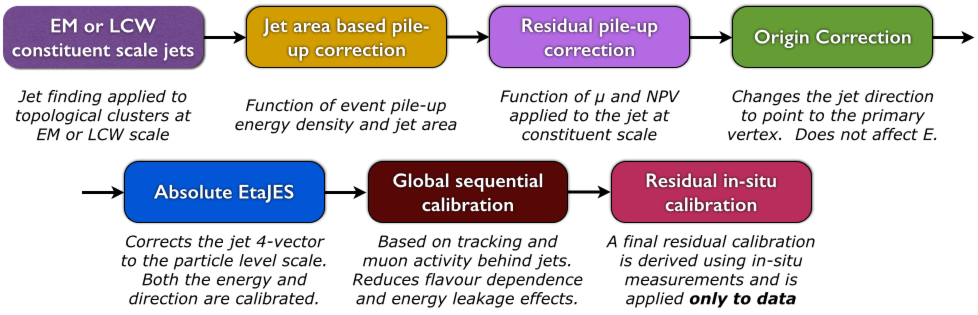
\includegraphics[width=15cm]{./fig/calib.png}	\caption{Overview scheme of jet calibration in the ATLAS.}
	\label{Fig.calib}
\end{figure}

\subsubsection{Pile-up corrections}


In order to eliminate a great amount of energy deposits from pile-up, a jet area-based subtraction of pile-up contribution to the \pt of each jet per event is applied as the start of the calibration chain. 

After all pile-up corrections are applied, the jet \pt~is given by:

\begin{equation}
p_{\mathrm{T}}^{\text {corr }}=p_{\mathrm{T}}^{\text {reco }}-\rho \times A-\alpha \times\left(N_{\mathrm{PV}}-1\right)-\beta \times \mu
\end{equation}
where $p_{\mathrm{T}}^{\text {reco }}$ indicates the reconstructed jet \pt~before any pile-up correction is applied. The jet area $A$ is defined by certain number of ghost tracks associated with a jet after clustering thus can quantify the liability of a jet to pile-up.  The pile-up \pt~density $\rho$ is used to evaluate the contribution from pile-up in the y-$\phi$ plane. To calculate the density $\rho$ of each jet in the distribution $\pt/A$, a $k_t$ algorithm with radius $R$ = 0.4 is employed to reconstruct jet from positive-energy topo-clusters within the range of \abseta < 2. The calculation of $\rho$ performed in such $\eta$ range for pile-up measurement is due to the fact that $\rho$ tend to be zero beyond \abseta~$\approx$ 2 as a result of lower occupancy in coarser segmentation in the forward region. Therefore, pile-up sensitivity in the forward region is not fully described after such correction.  

An additional residual correction is thus applied from the MC simulation to account for the difference between the reconstructed jet \pt~and truth jet \pt~as a function of the number of reconstructed primary vertices in the event $N_{\mathrm{PV}$  and the mean number of interactions per bunch crossing $\mu$, which are sensitive to in-time and out-of-time pile-up, separately. 

Both the initial values of $\alpha$ and $\beta$ coefficients are derived in bins of truth jet \pt~and geometric centre of the detector $|\eta_{det}|$. A logarithmic dependence on truth jet \pt~is observed.


\subsubsection{Jet energy scale and $\eta$ calibration}

Following the pile-up mitigation, the absolute jet energy scale and $\eta$ calibration are introduced to correct the four-momentum of the reconstructed jet to the truth-particle jets, accounting for defecting calorimeter response, energy losses when particles passed through certain materials, boundary effects and biases in the reconstructed jet in different $\eta$ due to the transition between the granularities and technologies changes in calorimeter. 


Since the detector responses differ across the detector $\eta$ range, the reconstructed jets are thus divided into small bins of $\eta_{det}$ and the energy of the truth jet $E^{truth}$ as the response distribution for fixed $E^{truth}$ is Gaussian. The average jet energy response $\mathcal{R}$ is defined as $E^{\text {reco }} / E^{\text {true }}$ using  the mean of a Gaussian fit in $\eta_{det}$ and $E^{truth}$ bins, and is further parameterized as a function of $E^{reco}$. Such response for PFlow jets is higher than that for EMtopo jet at low energies as the tracking information is considered. 


Besides Jet energy scale (JES) correction, the bias from the $\eta$ of the reconstructed jet to that of the truth jet is taken into account. The bias is defined as a significant deviation from zero in the signed difference between the reconstructed jet $\eta^{reco}$ and truth jet $\eta^{truth}$, separately. Then a second correction is applied as such difference is parameterized as a function of $\eta_{det}$ and $E^{truth}$.

 The calibration is derived as a function of energy and $\eta$ from the MC samples which do not have the effects from pile-up, and only correct the jet \pt~and $\eta$ instead of full four-momentum. The EMtopo and PFlow jets after full JES and $\eta$ calibration are regarded as EM+JES scale and PFlow+JES scale, respectively. Small non-closures beyond $|\eta_{det}|$ $\approx$ 3.2 in the calibration are seen due to approximate treatment of hadronic showers in the forward region, lead to an additional systematic uncertainty.


\subsubsection{Global sequential calibration}

The global sequential calibration (GSC), based the global jet observables such as the the fraction of jet energy measured in the different layer of hadronic and the EM calorimeters, the tracking information associated with the jets, and the number of muon track segment. For each observable, a series of multiplicative corrections are applied on the four-momentum as a function of $\pt^{truth}$ and $|\eta_{det}|$.  Considered any observable $x$, the correction is derived from the inverted jet response $\mathcal{R}$:

\begin{equation}
C(x)=\frac{\mathcal{R}^{-1}}{\left\langle\mathcal{R}^{-1}(x)\right\rangle}
\end{equation}
where $\left\langle\mathcal{R}\right\rangle$ is the average jet response. 

As a result, the fluctuations in the jet particle composition are reduced and the jet resolution can be improved without changing the average jet energy response which depends on the flavour and the energy distribution of the constituent particles. The shape of a jet varies between quark- and gluon-initiated jets as hadrons are often included in a quark-initiated jet with higher fraction of the jet \pt~with higher calorimeter response.

After applied GSC for PFlow jet, the average jet \pt~ response on each observable is reduced to lower than 2\% with small deviations from correlations between observables.


The fractional jet resolution $\sigma_{\mathcal{R}} / \mathcal{R}$ is derived from the jet resolution $\sigma_{\mathcal{R}}$, which is defined by the standard deviation of a Gaussian fit to the distributionof  jet \pt~response. This fractional jet resolution is used to determine the size of the fluctuations in the jet energy reconstruction.



\subsubsection{Residual $in~situ$ calibration}

The final step of the jet calibration is performed only in data to account for the differences of jet response measurement in data and the MC, the derived ratio of it is used as a correction in data.
The differences are introduced by the inadequate nature of the detector materials and the imperfect simulation of the real physics processes. Such differences can be quantified by weighting the \pt~ of a jet to other reference objects that well-measured. The correction factor  can be denoted as follows:
\begin{equation}
c=\frac{\mathcal{R}_{\text {in situ }}^{\text {data }}}{\mathcal{R}_{\text {in situ }}^{\mathrm{MC}}}
\end{equation}
the response $\mathcal{R}_{\text {in situ}}$ represents the average ratio of the jet \pt~ to the reference object \pt~ in bins of reference object \pt, where the average value is founded from peak value of a Gaussian fit to the distribution. The double ratio is robust to secondary effects thus more reliable in term of the measurement of jet energy.

Three stages are carried out in such $in~situ$ calibration. First, $\eta$-intercalibration is performed on the energy scale of forward jets (0.8 $\leq |\eta_{det}|$ < 4.5) to match the central jets ($|\eta_{det}|$ < 0.8) using the jet \pt~in dijet events. Then $Z$+jet and $\gamma$+jet analyses balance the measurement of \pt~response of a well-calibrated $Z$ boson or photon. Finally, a multijet balance (MJB) analysis is employed to calibrate low-\pt~jets to a very high-\pt~jet. Both MJB and $Z/\gamma$+jet analyses are used only for jets in the central region (\abseta < 1.2). All three $in~situ$ calibrations are done sequentially so that the systematic uncertainties can be propagated from each to the next. The systematic uncertainties in each calibration process come from three sources: the MC modelling of physics processes, the uncertainties in the measurement and from topology obtained by different event selections.







%  Since the momentum is conserved throughout the showering and the hadronization process, a parton with large momentum will thus product particles which also have a signification fraction of their momenta in that direction. These final-state hadrons can be grouped into a spray of particles in the same region of the detector. A jet can thus be form by gathering the final-state particles and their energies into a single object. The finding of a jet goes back to a seminal work done by G. Sterman and S. Weinberg [68]. No standardized procedure for the jet finding algorithms exist, but there are a set of properties considered to be important [69]:

%Jets in ATLAS can be defined using a variety of objects. Truth-particle jets are formed using stable particles with lifetimes longer than 10 ps excluding muons and neutrinos from the event generator. Track jets are built from charged particle tracks in inner-detector. They are insensitive to the effect of pile-up. And last the calorimeter jets which are used most commonly by analysis, use the topocluster for reconstructions [70].
%In this chapter, two algorithms employed in the ATLAS will be discussed following the reconstruction. A brief introduction to the jet calibration will also be presented.

\newpage
\fancyhead[C]{The calibration of quark/gluon jets taggers}
\section{The calibration of quark/gluon jets taggers}
\label{sec:5}
The classification of jets originated from a quark or a gluon is useful for improving the SM measurements and searches for BSM physics at the LHC.  According to the QCD,  gluons are in the adjoint representation of the $SU(3)$ gauge group thus carry both colour and anti-colour quantum numbers, whereas quarks are in the fundamental representation and have only a single colour number~\cite{ALTARELLI1977298}. As a result, a gluon-initiated jet (gluon-jet) tend to have more constituents and a broader radiation pattern than a quark-initiated jet (quark-jets). 

The manifestation of colour charges is intrinsic to quarks and gluons; however, the confinement phenomenon inherent in QCD theory indicates that only colour neutral hadrons can be observed in the detector. Such principle brings significant challenges for the identification of quark- or gluon-jets in ATLAS. The identification method relies on the number of charged tracks within the jets and the reconstruction algorithm for it. The calibration described in this paper demonstrates the measurement of the tagging efficiencies of the aforementioned jet taggers. The more advanced boosted decision tree (BDT) algorithm is employed to constructed the jet tagging variable based on the charge multiplicity inside jets. A matrix method is established with the use of quark/gluon fraction in quark-/gluon-enriched subsamples, defined by the pseudorapidity of jets. The scale factors extracted from the difference between data and simulation are provided for tagger working points corresponding to 50\%, 60\%, 70\% and 80\% fixed quark-jet efficiencies for both quark- and gluon-jets, respectively.
  

In addition to earlier investigations that concentrated on single-variable taggers within a lower \pt~range~\cite{Aad_2014,ATL-PHYS-PUB-2017-009}, this research emphasizes the development of a novel $q/g$ tagger that incorporates multiple jet substructure parameters. Additionally, it aims to expand the application of $q/g$ tagging to a broader energy spectrum.

\subsection{Data and Monte Carlo samples}
\label{sec:Data-MC}

\subsubsection{Data}
\label{subsec:data}
The data recorded in 2015-2018 with integrated luminosity of 140 \ifb (full Run 2 data) is used in this study. The data samples are processed through the un-skimmed DAOD\_JETM1 derivation scheme in order to obtain multi-jet events. The lowest un-prescaled small-$R$ single-jet trigger is employed for this analysis. The jet \pt~threshold for the trigger in this analysis is 420 GeV, keeping the selection consistent across years, together with additional requirements that ensure events of good qualities are used. The additional selections are:
\begin{itemize}
	\item Good Run List (GRL): Make sure a steady state of all relevant detectors so that physics processes recorded by them are good.
	\item LAr: Liquid Argon Calorimeter error rejected.
	\item Tile: Tile Calorimeter error rejected.
	\item SCT: SCT single event upsets rejected.
	\item Core: Incomplete event build rejected.
	\item Primary Vertex: the highest $\sum\pt^{2}(trk)$ vertex has at least two tracks associated with it
	\item Trigger: Passes the lowest unprescaled single-jet trigger, HLT\_j420
\end{itemize}

Additional kinematic selection criteria are  discussed in Section~\ref{sec:Obj-event}.


\subsubsection{Monte Carlo simulation}
\label{subsec:MC}

For this calibration, multi-jet events are generated and modelled with several MC simulations, processed through the same DAOD\_JETM1 derivation scheme. For the nominal result, \pythia8.230 MC generator is used with leading-order (LO) matrix element (ME) for dijet production. Parton density functions (PDFs) are considered for systematic uncertainties evaluation as the \nnpdftwoLO PDF set is used for \pythia8.230.  Alternative samples with different choices of parton shower modelling, ME generation,  and the simulation of the multi-parton interactions are included to estimate the systematic uncertainties.

Two set of MC samples generated using \sherpa2.2.5 are used with the same ME for the (2$\rightarrow$2) process at LO, to provide the uncertainties of hadronization modeling. The \ctten PDF sets are included in both \sherpa samples where one based on the cluster hadronization whereas the other used \sherpa interface to the Lund string fragmentation model as \pythia8.230.

Two set of MC samples generated using \herwig7.1.3 are used for parton shower uncertainties as one uses angular ordering shower whereas the other one uses dipole shower. These samples are produced at next-to-leading order (NLO) with a PDF set of \mmht.


Another set of multijet samples that produced with \powheg interfaced to \pythia at NLO accuracy is employed with \nnpdftwo LO PDF set, to estimate the effects from the ME uncertainty as different perturbative scales in the ME and parton distribution functions are included. The renormalization and factorisation scales are set to the \pt~of the underlying Born configuration. These samples included different perturbative scales in the ME and parton distribution functions are used for the estimation of ME uncertainty.


%In this study, several multi-jet samples after JETM1 DAOD un-skimmed derivation with different modelings are used. %The parton shower modeling of the Monte Carlo~(MC) simulation is \pythia8 \cite{Sjostrand:2014zea} and \sherpa \cite{Gleisberg:2008ta}. %There are Pythia8 and Sherpa 2.2.5 samples which include both Scale and Parton Density Function~(PDF) variations. To flatten statistics across lower-pT slices, where the drop in cross section with increasing pT is greatest, weighted (JZW) filtering has been applied to the four lowest-pT slices. Slices JZ5 - JZ9plus are with JZ slicing. 

%There are 2 sets of Sherpa samples with the same Matrix Element~(ME) and shower configurations but different hadronization, which can be used for the estimation of uncertainties coming from fragmentation.

%Apart from these, there are Herwig 7.1 NLO~\cite{Bellm:2015jjp} samples (from JZ1 to JZ9plus) including scale variations from hard scattering and shower. There are 2 set of Herwig samples with same ME and hadronization but different types of showers, which can be used to investigate the effects of the parton shower modeling.
A list of the MC samples used is given in table~\ref{tab:MC}.




\begin{table}[H]
%\tiny
%\renewcommand{\arraystretch}{1.2}
\begin{center}
\begin{tabular}{ |c |c |c| c | c |}
  \hline
  PDF set & Generator      & Cross-section& Parton shower & Hadronisation \\ 
  \hline

\nnpdftwo              & \pythia8.230
         & LO            & \pt-ordered  & String \\
  \hline                                                                                                                                                              
\ctten                     & \sherpa2.2.5   & LO           & \pt-ordered  &Cluste      \\
  \hline
\ctten                     & \sherpa2.2.5   & LO           & \pt-ordered  & String \\
  \hline
 \mmht
  & \herwig7.1.3   & NLO           & Dipole & Cluster   \\
  \hline
\mmht
  & \herwig7.1.3   & NLO           & Angular-ordered & Cluster   \\
 \hline
\nnpdftwo
& Powheg+\pythia  & NLO         &   \pt-ordered  & String    \\
  \hline
\end{tabular}
\caption{The MC simulation used for the multi-jet processes in this calibration. %
	The PDF sets, generators for a hard process, the order in $\alpha_{\mrm s}$ of cross-section calculations and the simulator of parton showers, %
	and hadronisation are shown. }
\footnotesize
\label{tab:MC}
\end{center}
\end{table}






\subsection{Object and Event selection}
\label{sec:Obj-event}
In order to perform the calibration of the quark-/gluon-jet tagger, it is requisite to establish two distinct subsamples. One subsample should be predominantly composed of quark-jets, called quark-enriched sample, while the other should predominantly consist of gluon-jets, as gluon-enriched sample. These subsamples are gained from the dijet events. This section describes the reconstruction and selection of jet objects used in this calibration, as well as the approach to construct quark- and gluon-enriched subsamples.

\subsubsection{Physics object definition}
\label{subsec:obj}

The PFlow jets that are reconstructed with the \antikt~algorithm with a radius parameter $R$ set to 0.4. An overall jet energy calibration described in section~\ref{sec:4.2} has been done to rectify residual detector effects and pile-up. In order to ensure a good quality jet, an event-based jet cleaning with standard loose cut is applied to reject events with flawed leading or subleading jet.

Tracks that reconstructed~\cite{ATLAS:2017kyn} from the ID are required to have \pt~> 500 MeV, and within the ID range \abseta < 2.5. Additional criteria such as primary vertex are required to ensure selected tracks originating from the collision and prevent the mis-reconstructed tracks from pile-up hits in the detector. The alignment of tracks with calorimeter-based jets is executed through the application of the ghost-association technique. This entails a repetition of the jet clustering procedure augmented by the inclusion of 'ghost' representations of registered tracks~\cite{CACCIARI2008119}. These ghost tracks share the same direction as their actual counterparts but possess an infinitesimally small \pt, thereby ensuring that they do not induce any alterations to the intrinsic characteristics of the calorimeter-based jets. A criterion for track-jet correspondence is established: a given track is associated to a jet if its corresponding ghost track is contained in the jet after reclustering.


Jet reconstructed from the simulated MC is known as "truth jets"~\cite{ATLAS:2020cli}, with the same \antikt $R=0.4$ algorithm as PFlow jets. Geometric correspondence between truth jets and PFlow jets is established via angular proximity, adhering to the criterion $\Delta R < 0.4$. Each truth jet is bestowed with a flavour label, referred to as a truth label~\cite{Aad_2014,ATL-PHYS-PUB-2017-009}. The truth flavour label attributed to a jet is defined by the flavour of the highest-energy parton situated within a cone of size $\Delta R < 0.4$ around the jet's axis, prior to the process of hadronisation in the parton shower. Following this definition, jets arising from the splintering of gluons into $b$- or $c$-quark pairs are labelled as heavy flavour jets. These heavy flavour jets are often identifiable by the long-lived or leptonically decaying hadrons. Therefore, no distinct discriminant tailored for heavy-flavour quarks is investigated within the current framework~\cite{CDF:2008ixu,ATLAS:2013uet}. Jets will be unlabelled if there is no corresponding truth parton with \pt $>$ 1 GeV is found within the cone surrounding the truth jet. These instances of unlabelled jets commonly emerge as a consequence of pile-up effects, and less than 1\% of the dataset used. They are thus ignored~\cite{ATLAS:2012mwf}.
 
 
  %through the following procedure: first, they are matched to the highest energy $b$-quark parton within $R$ = 0.3 of the truth jet axis. If one is found, the jet is labelled as a truth $b$-jet. If no $b$-quark parton is found, the procedure is repeated with $c$-quark partons. Both the $b$- and $c$-quark partons must have a \pt greater than 5 GeV. If no $c$-quark parton is found, then the highest energy light quark or gluon parton within a cone of R = 0.4 is used to assign the jet either a light quark or gluon label. Under this definition jets which originate from gluons splitting into $b$ or $c$-quark pairs will be labelled as heavy flavour jets. Because they are a small fraction of the overall event sample, any difference between jets arising from gluon splitting and direct production can be safely ignored. Jets can be unlabelled if no truth parton with \pt~> 1 GeV is found within the cone. Unlabelled jets, which are ignored, are less than 1\% at \pt~> 50 GeV . Only light quarks and gluons are considered in this jet tagging calibration..









\subsubsection{Event Selection and definition of quark and gluon-enriched samples}
\label{subsec:Event}

Events are chosen by the single-jet trigger, HLT\_j420. The jet \pt~is  required to be greater than 500 GeV, as more quark-jets and better resolution on the jet constituents are given. Only the leading two jets with the highest \pt~are used, as dijet events, and are required to be  \abseta~< 2.5 so that their charged constituents are collected within the coverage of the ID. To maintain the equilibrium in \pt~and suppress non-isolated jets, a criterion demands that the ratio of the \pt~of the leading jet to that of the sub-leading jet remains within 1.5. The two leading \pt~jets serve as the cornerstone for the formulation of quark-enriched and gluon-enriched subsamples.

The quark-enriched sample is derived from the jet with higher \abseta~among the leading two jets, while the gluon-enriched sample is extracted from the jet with lower \abseta. This selection strategy capitalizes on the intrinsic behaviour of PDFs at higher proton momentum fraction range, where there exists a higher likelihood of encompassing valence quark-jets. Consequently, jets situated in more forward regions (higher \abseta) have a higher probability of being quark-jets, while jets positioned closer to the central region (lower \abseta) manifest an increased likelihood of corresponding to gluon-jets~\cite{ATLAS:2015rlw}.







\begin{table}[htb]
	\centering
	
\begin{tabular}{|c|c|}
	\hline
	Selection & Multi-jet sample  \\ 
	\hline
	 Trigger    & HLT\_j420 \\ 
	 Number of jets         & $\geq2$ \\ 
	 $\pt(j_1)$             & $>500$ \\ 
	 $\pt(j_2)$             & $>500$ \\ 
	 $\pt(j_1)/\pt(j_2)$   & $<1.5$ \\ 
	 $|\eta(j_1)|$         &  $<2.1$   \\ 
	 $|\eta(j_2)|$         &  $<2.1$   \\ \hline
	 Target parton         & Quark(Higher \abseta )  or Gluon (Lower \abseta )       \\
	\hline
\end{tabular}
\caption{
	The selections to retrieve quark/gluon-enriched samples.
	"$j_i$" represents the $i$-th jet in \pt-ordering.
}
\label{tab:QG-sample}
\end{table}


The distribution of leading and subleading jets \pt~in dijet event after selections is shown in Figure~\ref{fig:QG-2samplePt} for both MC and data.




\begin{figure}[htb]
        \centering
        \subfloat[leading jet ]{\label{fig:QG-2samplePta}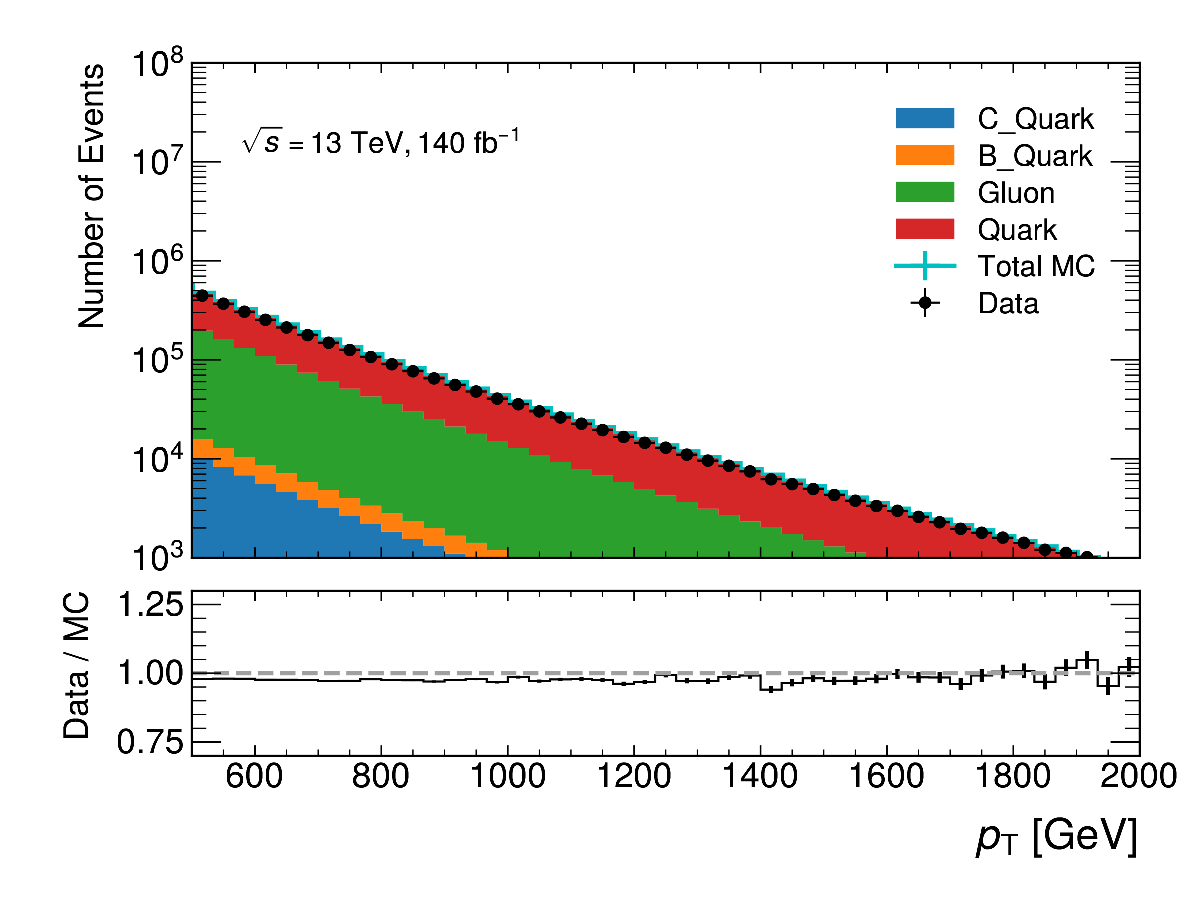
\includegraphics[width=0.48\textwidth]{fig/ADE/Pt_spectrum/none_event_weight/pt_MC16ADE_LeadingJet.pdf}} \quad
        \subfloat[subleading jet  ]{\label{fig:QG-2samplePtaa}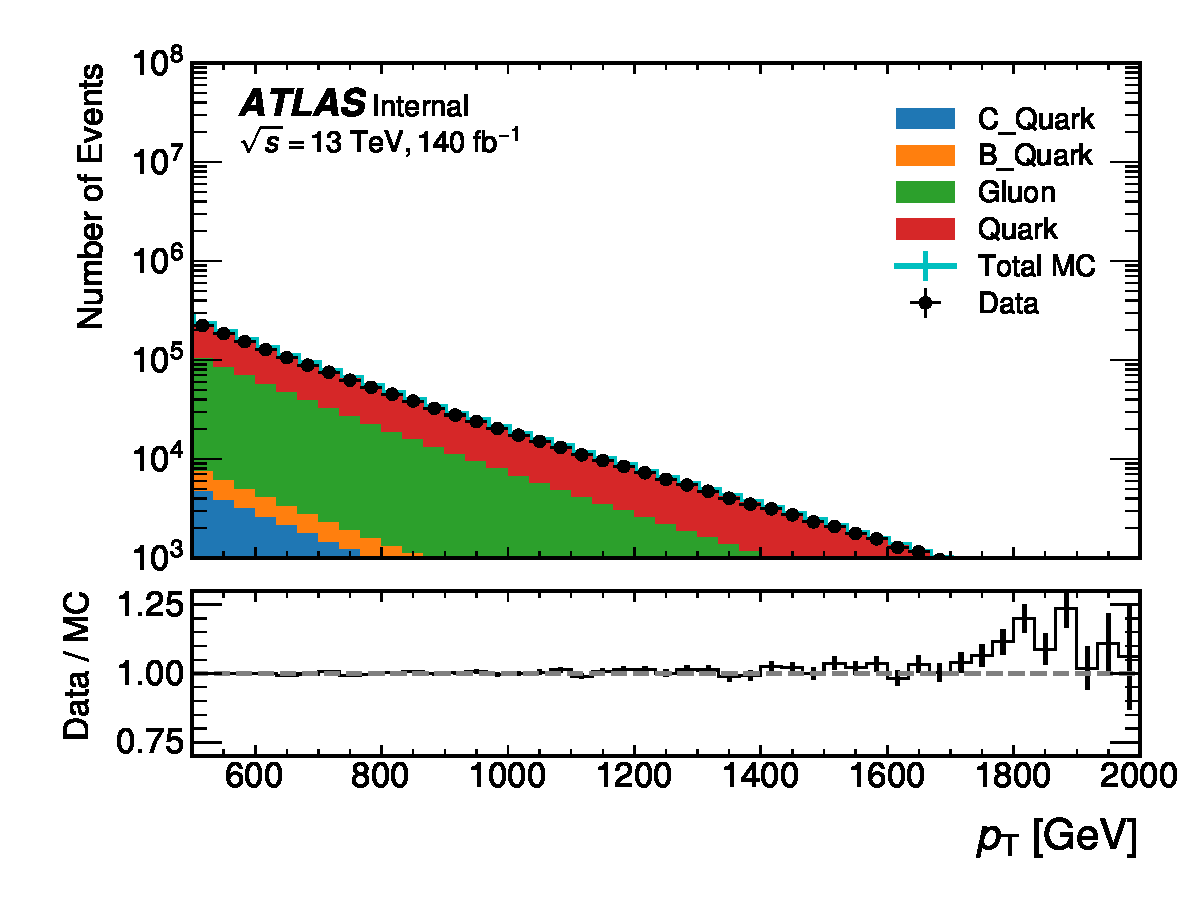
\includegraphics[width=0.48\textwidth]{fig/ADE/Pt_spectrum/none_event_weight/pt_MC16ADE_SubLeadingJet.pdf}} \quad
        \caption[]{
	  The \pt~distribution of the leading jets and sub-leading jets with \pythia samples for dijet event.
                \label{fig:QG-2samplePt}
        }
\end{figure}






\subsection{Quark/gluon tagging variables}
\label{sec:QG-var}
According to QCD, the colour factor of gluons is larger than that of quarks by factor 9/4 ("Casimir ratio")~\cite{ALTARELLI1977298}, which makes gluons emit more particles in the hadronisation than quarks. As a result, a gluon-initiated jet has more charged multiplicity associated and its width is larger than that of a quark-initiated jet. Therefore, the information of the track multiplicity inside a jet is crucial to distinguish quarks from gluons.

The $q/g$ tagging variables used in this study are based on the track multiplicity and are specified as : number of tracks ($\ntrk$), jet width (\wtrk)~\cite{Aad_2014,PhysRevLett.110.212001}, and two point energy correlation function (\cbeta)~\cite{Moult:2016cvt,Larkoski:2013eya} computed from the associated tracks. The expressions are defined as follows:

\begin{description}

  \item[\ntrk] \mbox{} \\
    \ntrk~is a number of tracks associated with the jet. %
    \begin{equation}
    \ntrk = \sum_{\mrm{trk}\in\mrm{jet}}
    \end{equation}

  \item[\wtrk] \mbox{} \\
    \wtrk~is a track-\pt-weighted width of the jet divided by the scalar sum of track transverse momenta. %
    It is defined as %
    \begin{equation}
      \wtrk = \frac{ \sum_{\mrm{trk}\in\mrm{jet}}\pttrk\Delta R_{\mrm{trk,jet}} }{ \sum_{\mrm{trk}\in\mrm{jet}}\pttrk },
    \end{equation}
    where \pttrk~is a \pt~of a charged track reconstructed by the ID and %
    $\Delta R_{\mrm{trk,jet}}$ is a distance in the $\eta-\phi$ plane between the track and the jet axis. %

  \item[\cbeta] \mbox{} \\
    Two point energy correlation function is defined as %
    \begin{equation}
      \cbeta = \frac{ \sum_{i, j\in\mrm{jet}}^{i\neq j} p_{\mrm{T}, i}p_{\mrm{T}, j} \left( \Delta R_{i,j} \right)^{\beta=0.2} }%
        { \left( \sum_{\mrm{trk}\in\mrm{jet}} \pttrk  \right)^{2} }, 
    \end{equation}
    where $i$ and $j$ denote tracks associated with the jet and the sum runs over all the combination of two tracks. % 
    The $\beta$ is fixed to $0.2$, which is known to be suitable for $q/g$ tagging.%~\cite{ref30}. % 

\end{description}

%\FloatBarrier
\subsubsection{The BDT tagger}

Multivariate Analysis (MVA) is a technique introduced to discriminate signal from background, one type of classification algorithm in MVA is the BDT. A tree structure is built to classify datasets through a sequence of branching binary decisions. Data with desirable features is kept by discriminating algorithm whereas others are rejected. Each decision point made construct a node at each level of the decision tree, and a score is assigned to every classifier that goes into the boosting process based on its error rate. One decision node can have two or more branches to split the datasets. Such procedure is iterated from top to down so that a termination condition such as the minimum number of samples in a node or a maximum depth in a tree depth is met. A diagram of a single decision tree is shown in Figure.~\ref{Fig.bdt}. After all series of cuts are applied, the BDT is defined. Therefore, a cut based on the BDT score can be employed as the most correct classification of datasets.

\begin{figure}[htb] 
	\centering  
	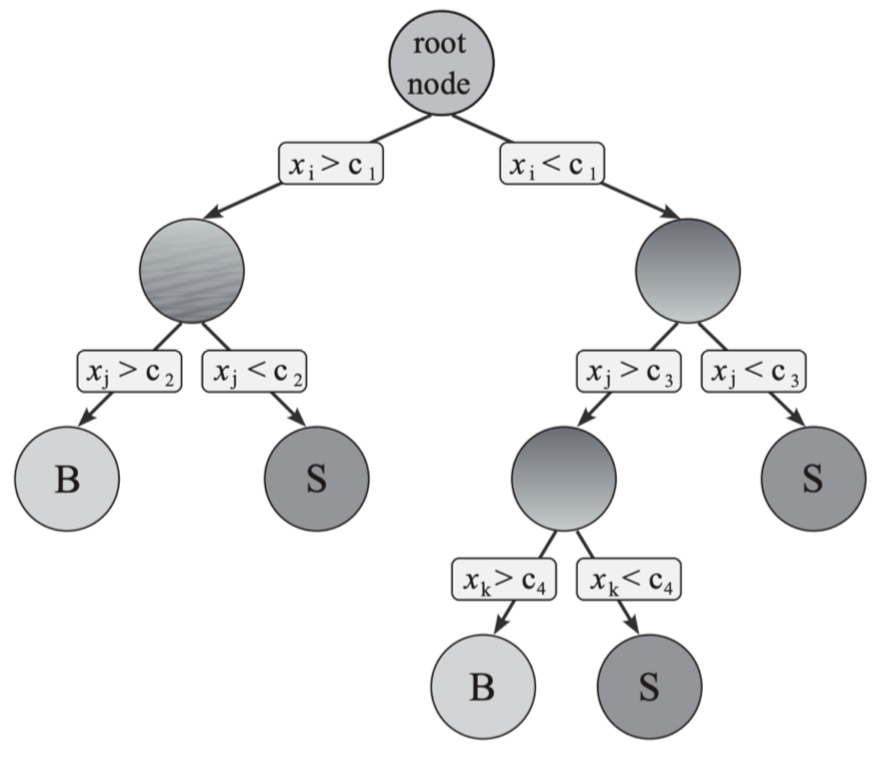
\includegraphics[width=11cm]{./fig/bdt.png}
	\caption{A scheme of a single decision tree with a depth of three}
	\label{Fig.bdt}
\end{figure}

The BDT tagger is constructed by the combination of tracking-related observables: \ntrk, \wtrk, \cbeta~and \pt~of a jet are included as the distribution of the track multiplicity is affected by them. In this study, the BDT score is used to classify quark- or gluon-jets from the multi jet samples, with the truth-labelled information from MC to train until a quark signal efficiency larger than 90\% is reached.


The BDT tagger is trained using the LGBMClassifier from lightGBM~\cite{NIPS2017_6449f44a} framework, and hyper-parameter tuning is performed with Optuna~\cite{akiba2019optuna}. The MC \pythia samples are employed.

An individual score is allocated to each BDT within the boosting procedure, factoring in its error rate.  This BDT score serves as the criterion for classifying a given jet as either a quark-jet or a gluon-jet. 

\paragraph{Feature selections}\mbox{}\par
Drawing upon the features employed during the training process, an exploration of the correlation matrix is undertaken to assess the interdependence among jet attributes, including \pt, \abseta, and jet substructure variables \ntrk, \wtrk, \cbeta, and the BDT. Figure~\ref{fig:weighted_corr} shows \ntrk, \wtrk~and \cbeta exhibit notable interrelationships among themselves, displaying relatively robust correlations. In contrast, \pt~and $\eta$ display a diminished level of correlation. The distributions of all single jet substructure variables and BDT score with systematic uncertainty in forward and central regions are shown in Figure~\ref{fig:QG-pythia-Unc_Ntrk-wp11}. The distributions of all single jet substructure variables and BDT score with systematic uncertainty of quark- and gluon-jets in different \pt~ranges from the MC simulation are shown in Figure~\ref{fig:QG-pythia-Unc_Ntrk-wp11q}.

\begin{figure}[htb]
	\centering
	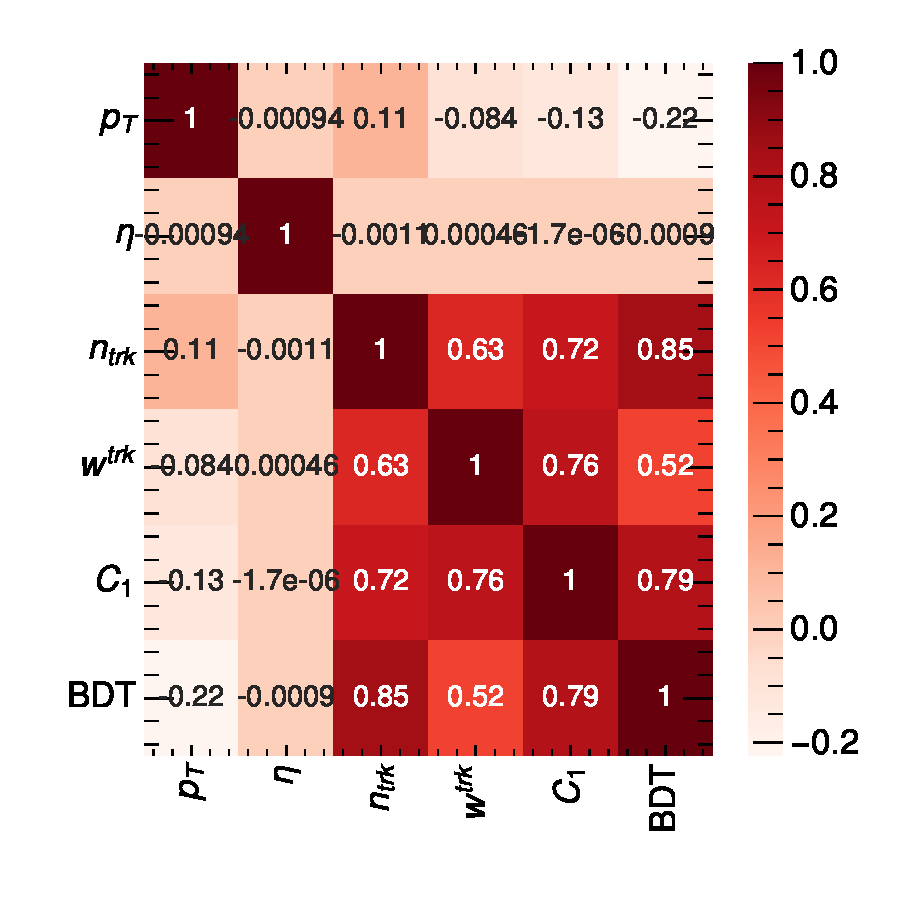
\includegraphics[width=0.65\textwidth]{fig/ADE/new_GBDT/corr.pdf}
	\caption{correlation matrix of jet variables.}
	\label{fig:weighted_corr}
\end{figure}

\begin{figure}[htbp]
	\centering
	\subfloat[]{\label{fig:QG-pythia-UncPythiaQa_Ntrk-wp1}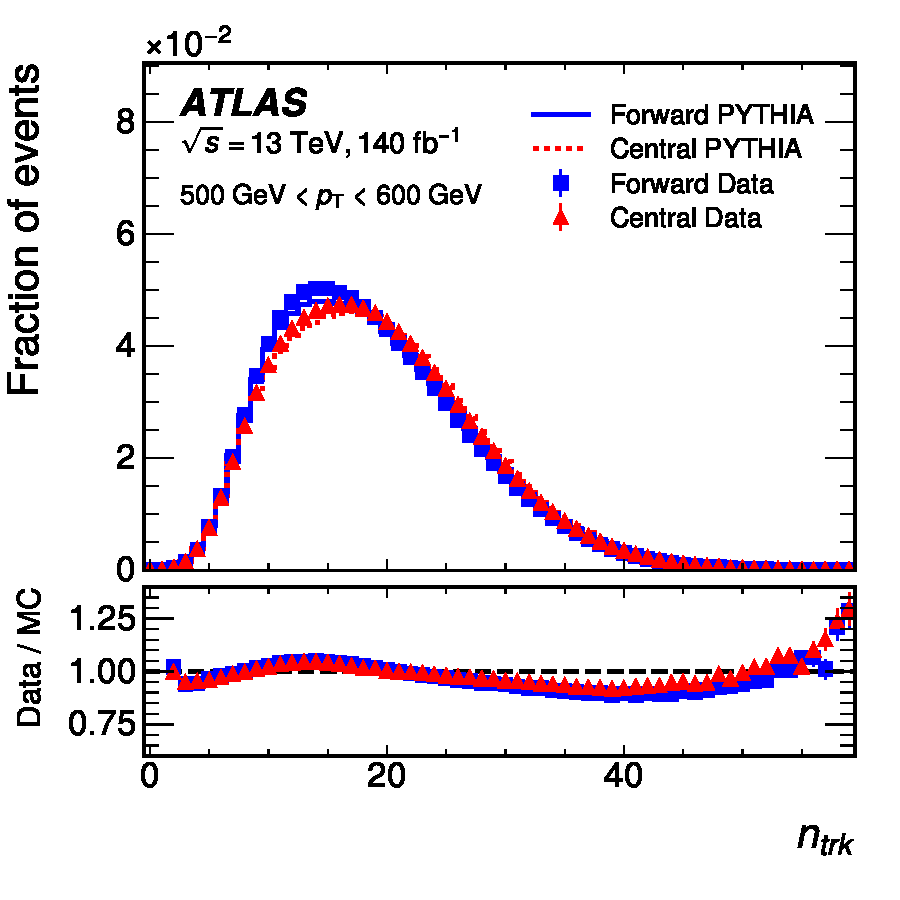
\includegraphics[width=0.45\textwidth]{fig/FvsC_syst/MCvsData_FvsC_500_none_reweight_jet_nTracks.pdf}}\quad
	\subfloat[]{\label{fig:QG-pythia-UncPythiaQb_Ntrk-wp2}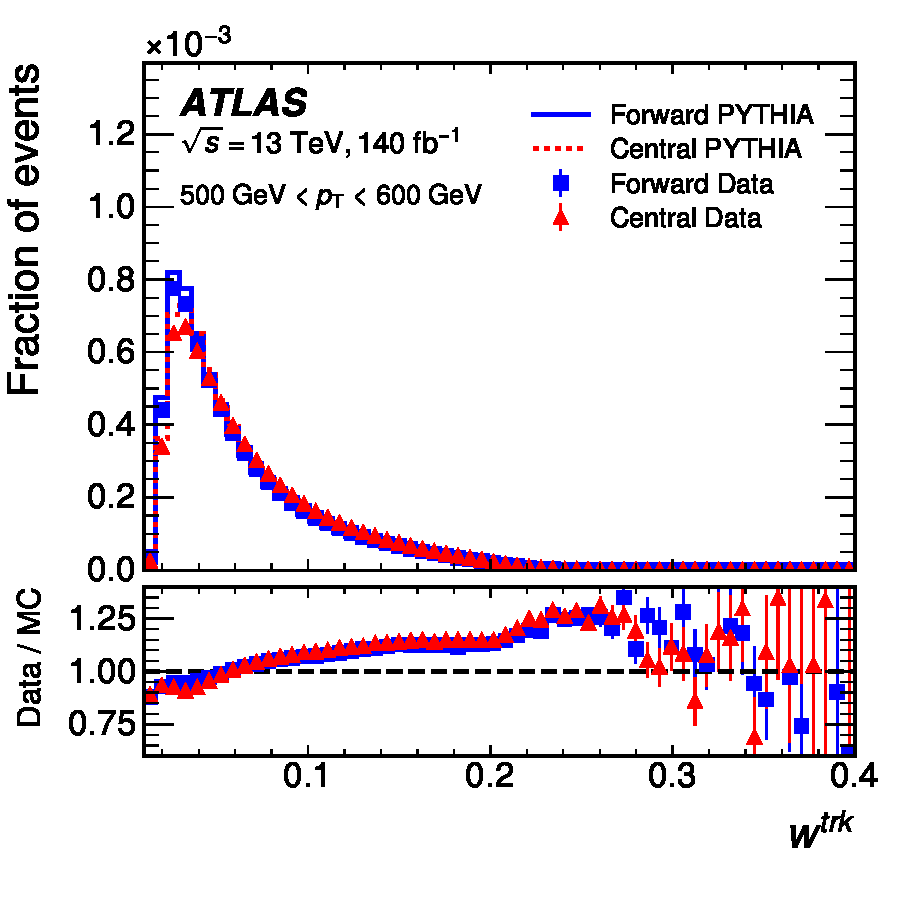
\includegraphics[width=0.45\textwidth]{fig/FvsC_syst/MCvsData_FvsC_500_none_reweight_jet_trackWidth.pdf}}\\
	\subfloat[]{\label{fig:QG-pythia-UncPythiaQa_Ntrk-wp3}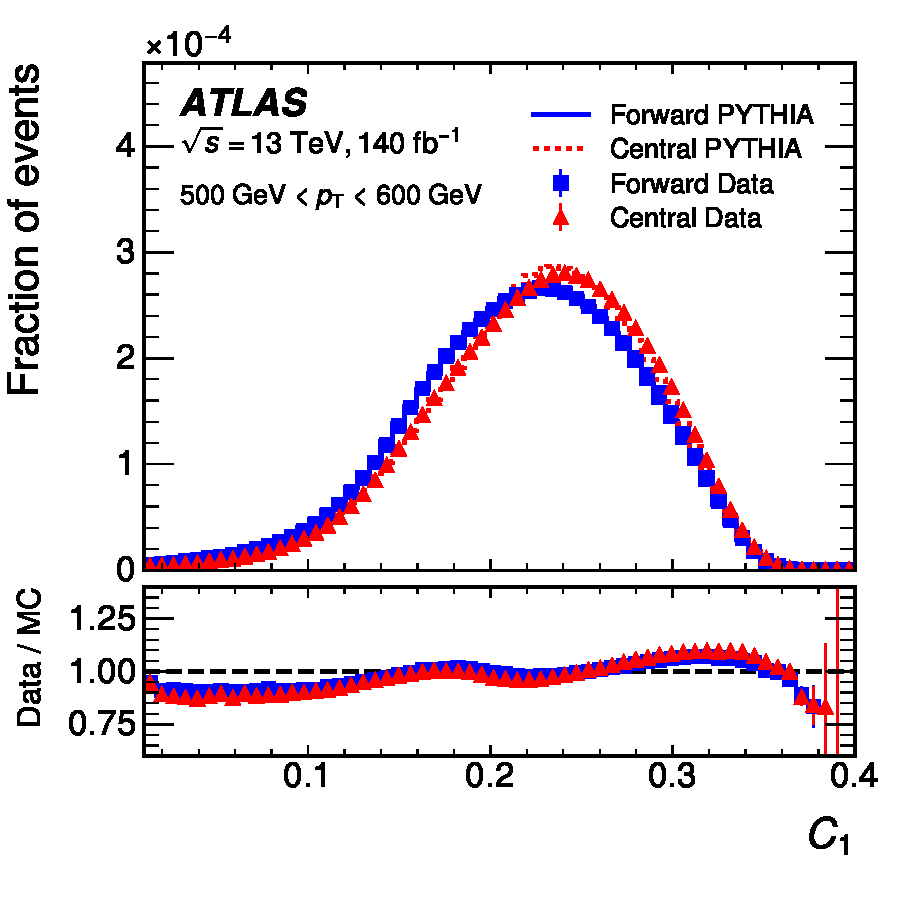
\includegraphics[width=0.45\textwidth]{fig/FvsC_syst/MCvsData_FvsC_500_none_reweight_jet_trackC1.pdf}}\quad
	\subfloat[]{\label{fig:QG-pythia-UncPythiaQb_Ntrk-wp4}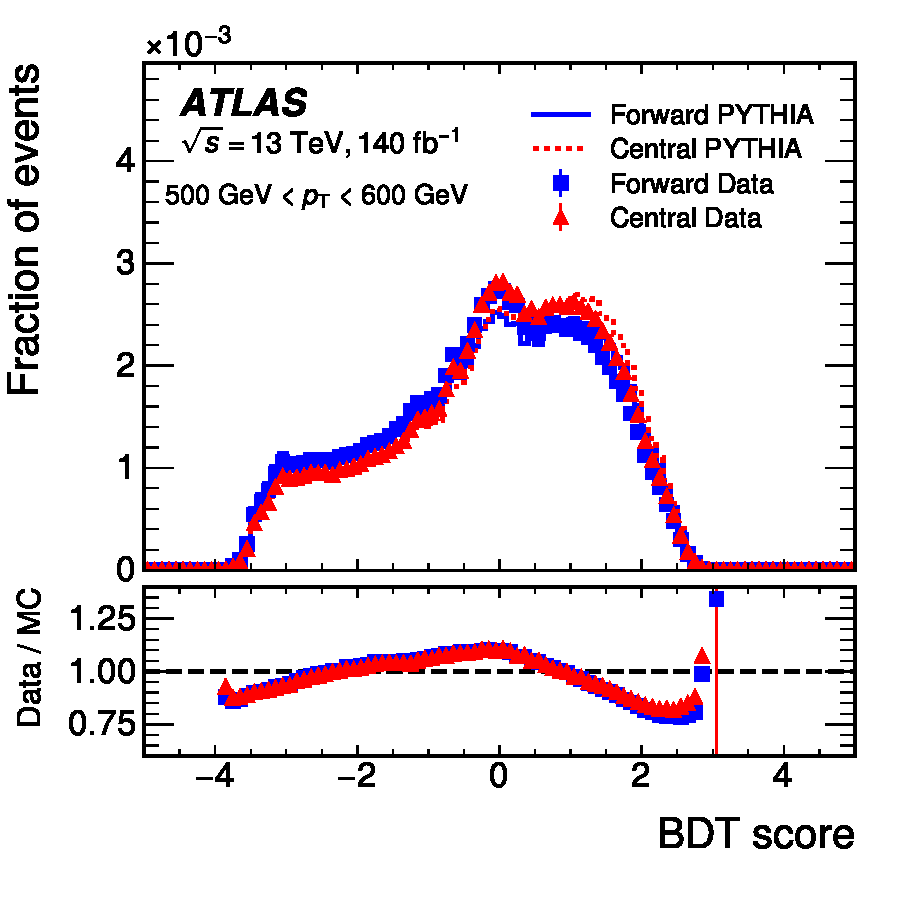
\includegraphics[width=0.45\textwidth]{fig/FvsC_syst/MCvsData_FvsC_500_none_reweight_GBDT_newScore.pdf}}
	\caption[]{
		The distributions of \ntrk~\subref{fig:QG-pythia-UncPythiaQa_Ntrk-wp1}, \wtrk~\subref{fig:QG-pythia-UncPythiaQb_Ntrk-wp2}, $C_1$~\subref{fig:QG-pythia-UncPythiaQa_Ntrk-wp3} and BDT score~\subref{fig:QG-pythia-UncPythiaQb_Ntrk-wp4} in the forward and central regions in data (closed symbols) and the \pythia MC (lines) are shown in the upper panels. The bottom panels show the ratio of the data and the MC. The distributions shown are for jet \pt~in the range between 500 GeV and  600 GeV. The vertical error bars show the statistical uncertainty.
		\label{fig:QG-pythia-Unc_Ntrk-wp11}
	}
\end{figure}


\begin{figure}[htbp]
	\centering
	\subfloat[]{\label{fig:QG-pythia-UncPythiaQa_Ntrk-wp1}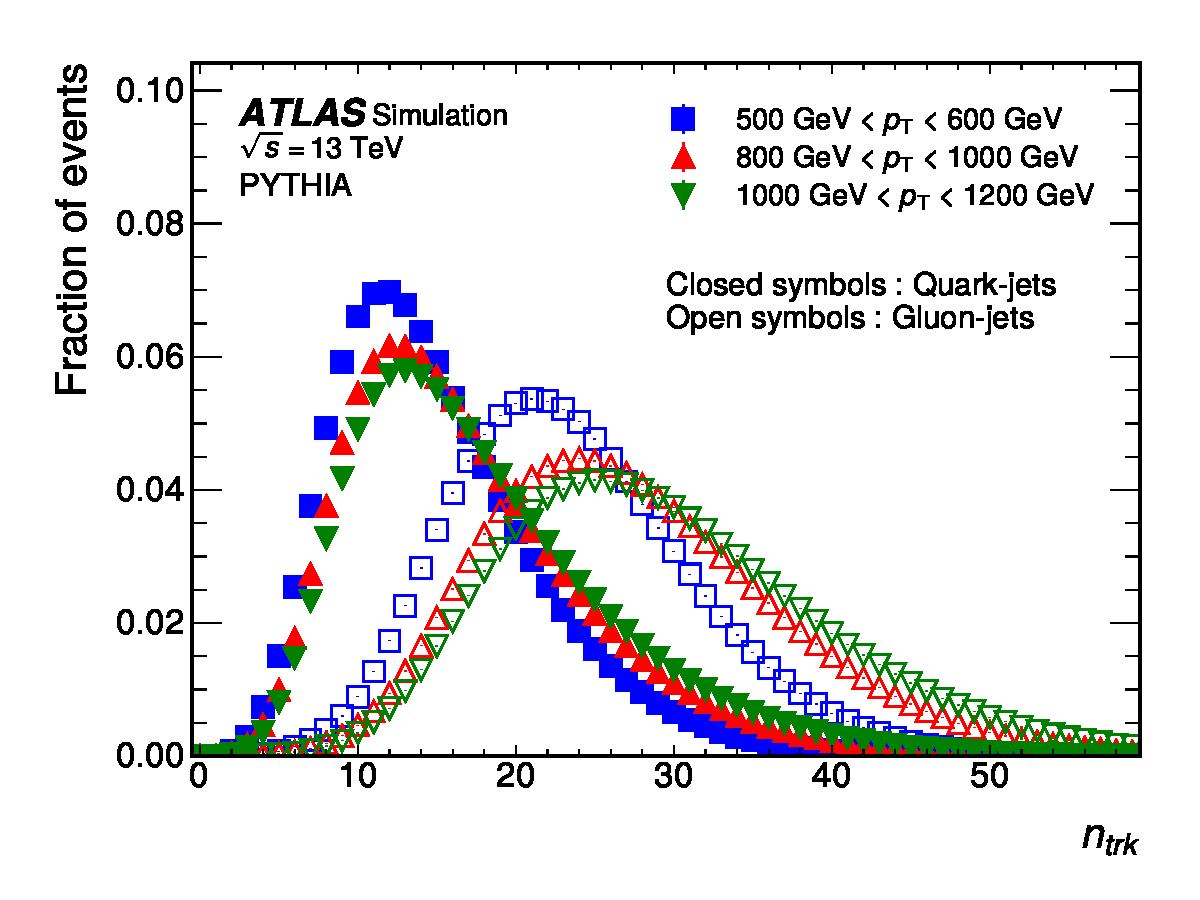
\includegraphics[width=0.45\textwidth]{fig/FvsC_syst/MCvsData_QvsG_1500_none_reweight_jet_nTracks_binned.pdf}}\quad
	\subfloat[]{\label{fig:QG-pythia-UncPythiaQb_Ntrk-wp2}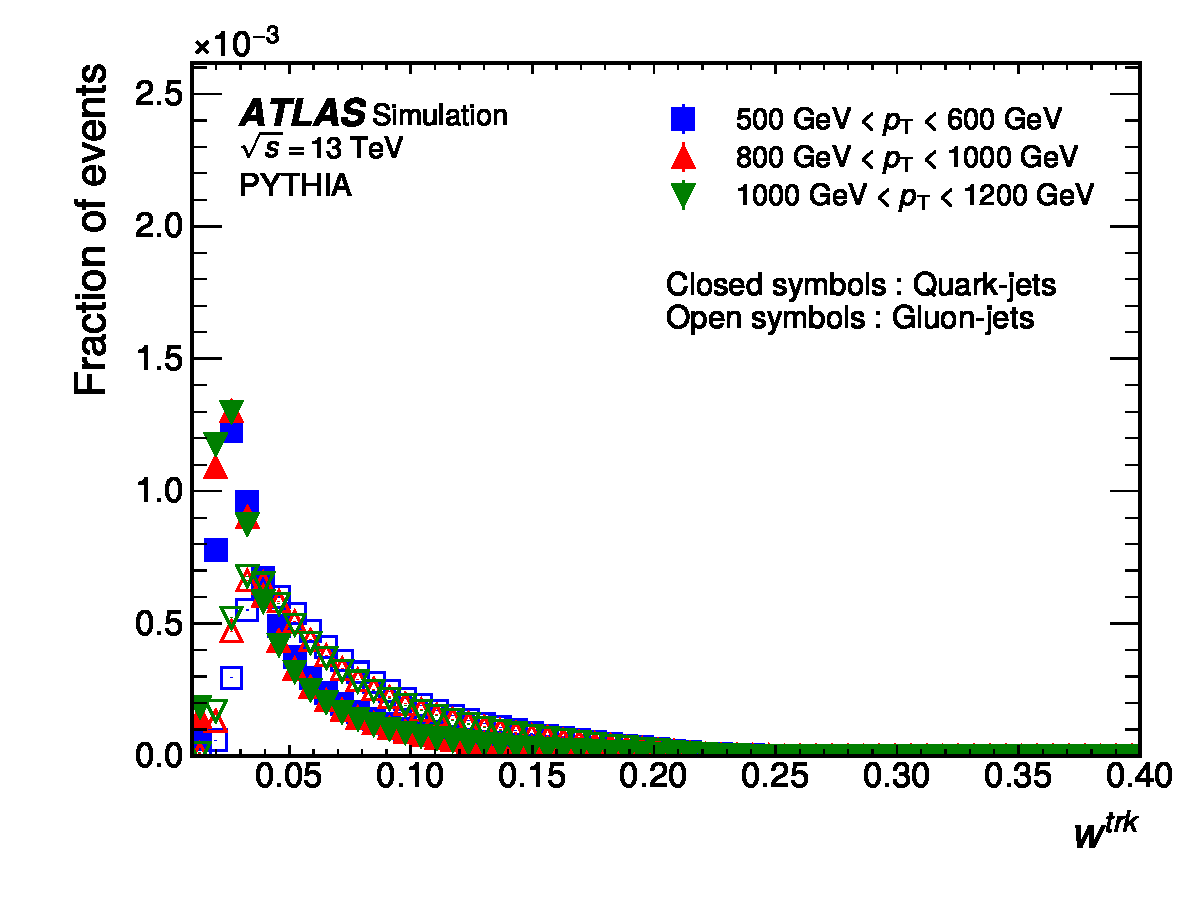
\includegraphics[width=0.45\textwidth]{fig/FvsC_syst/MCvsData_QvsG_1500_none_reweight_jet_trackWidth_binned.pdf}}\\
	\subfloat[]{\label{fig:QG-pythia-UncPythiaQa_Ntrk-wp3}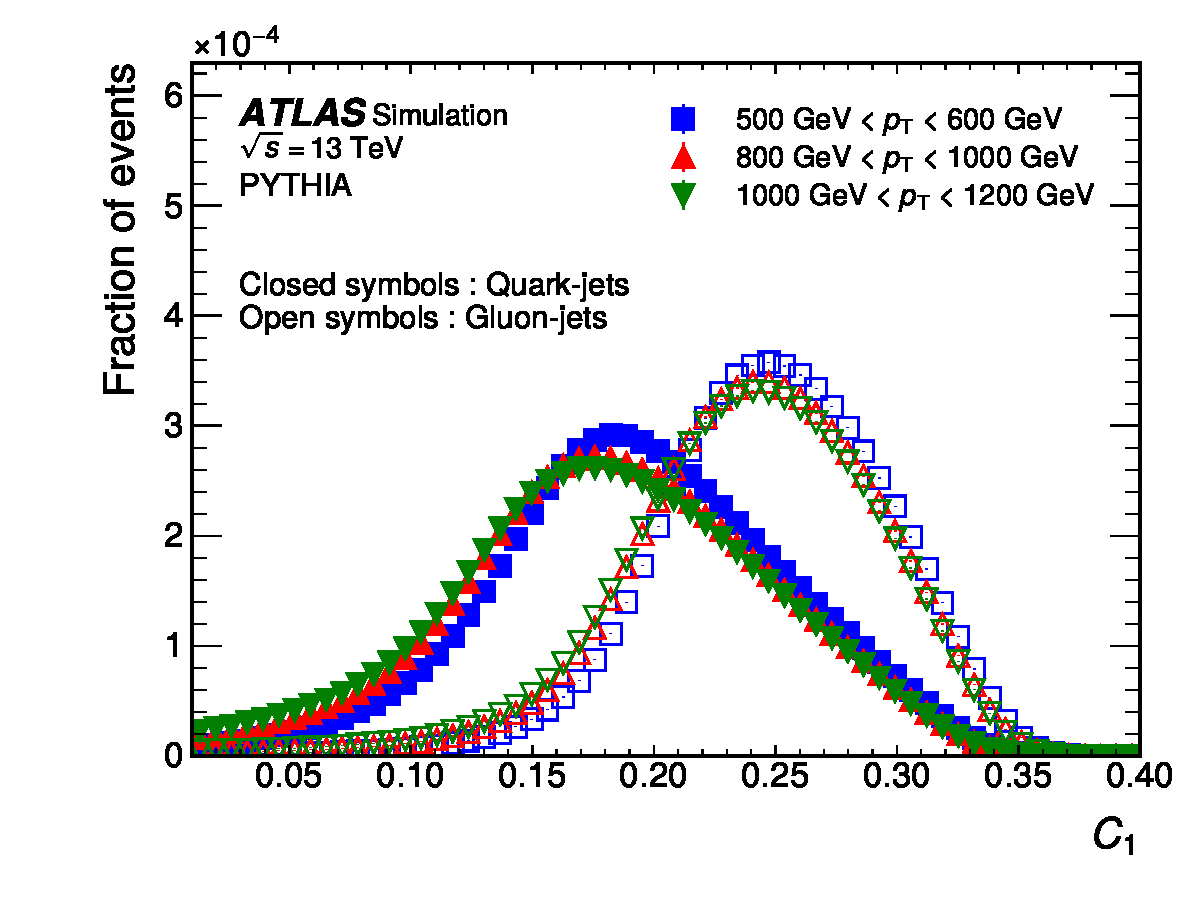
\includegraphics[width=0.45\textwidth]{fig/FvsC_syst/MCvsData_QvsG_1500_none_reweight_jet_trackC1_binned.pdf}}\quad
	\subfloat[]{\label{fig:QG-pythia-UncPythiaQb_Ntrk-wp4}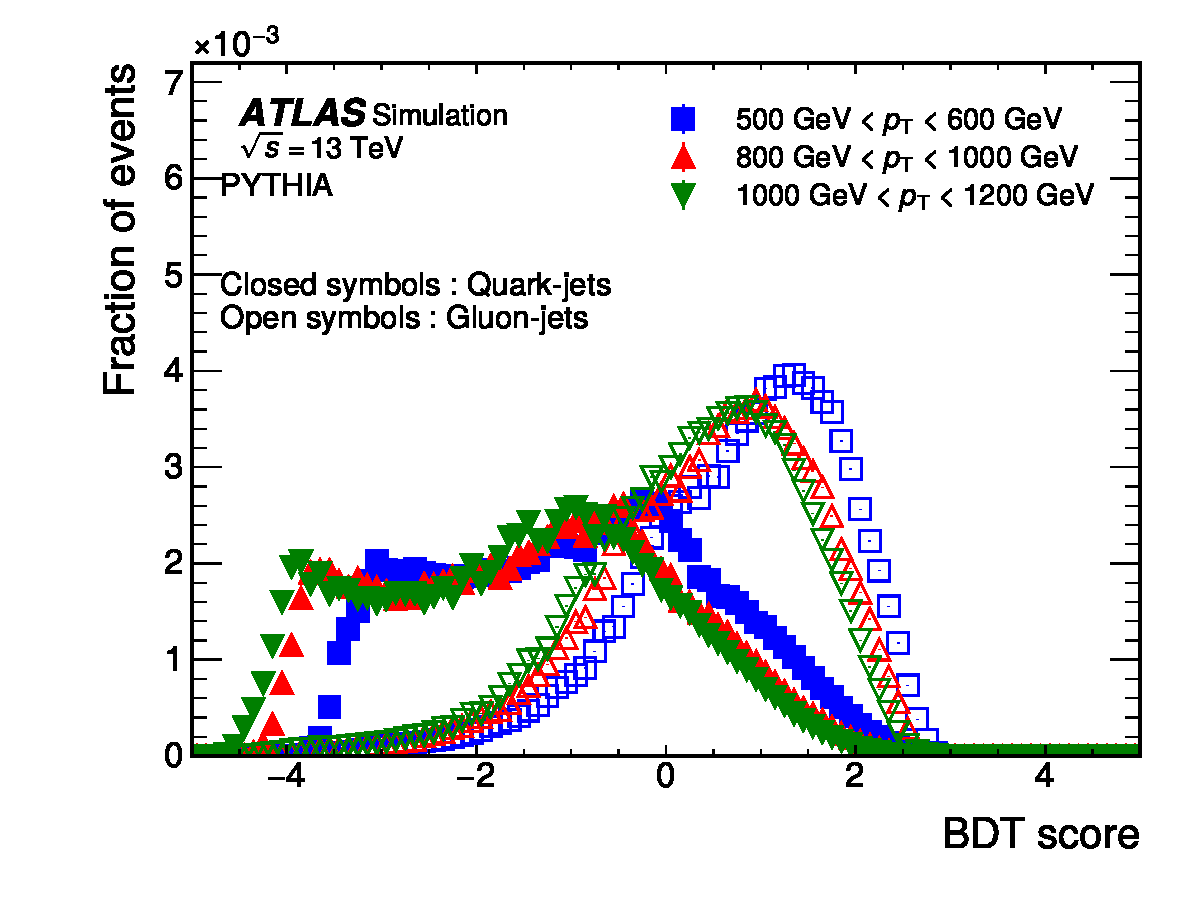
\includegraphics[width=0.45\textwidth]{fig/FvsC_syst/MCvsData_QvsG_1500_none_reweight_GBDT_newScore_binned.pdf}}
	\caption[]{
		The distributions of \ntrk~\subref{fig:QG-pythia-UncPythiaQa_Ntrk-wp1}, \wtrk~\subref{fig:QG-pythia-UncPythiaQb_Ntrk-wp2}, $C_1$~\subref{fig:QG-pythia-UncPythiaQa_Ntrk-wp3} and BDT score~\subref{fig:QG-pythia-UncPythiaQb_Ntrk-wp4} in the quark-jets (closed symbols) and gluon-jets (open symbols) in given \pt~regions using the \pythia MC samples.
		\label{fig:QG-pythia-Unc_Ntrk-wp11q}
	}
\end{figure}

Rather than employing multiple BDTs for different \pt~ranges, an universal BDT can be trained using events in all \pt~ranges.
Given the intrinsic correlation between \ntrk~and the jet \pt, a natural way to choose features is including \pt~in addition to three $q/g$ tagging variables.    
Concerning the remaining variable, $\eta$, two comparative scenarios are juxtaposed: one involves its inclusion, and the other pertains to its exclusion. This comparison facilitates an assessment of whether or not to incorporate \abseta.

\begin{enumerate}
	\item \pt, \ntrk, \wtrk~and \cbeta
	\item \pt, \abseta, \ntrk, \wtrk~and \cbeta
\end{enumerate}

The result depicted in Figure~\ref{fig:QG-training_scenario_compare_500_600} shows a distinct discrepancy when \abseta is encompassed within the training. 
This violates the assumptions that the partons distribution in more forward and more central regions should not change. Specifically, the distribution of BDT scores for forward quarks substantially diverges from that of central quarks, a trend that is similarly observed for gluons. Moreover, adopting the BDT tagger that incorporates \abseta~would result in inadequate performance for jets situated within the central region when this tagger is applied to a pure sample of quark-jets (e.g., $Z$+jet samples).
In the present analysis, the BDT is endowed with the spectra of \pt, \ntrk, \wtrk, and \cbeta, as exemplified in scenario 1. 
At detector-level, however, the observed radiation pattern within jets no longer remains unaffected by \abseta, owing to variances in the detector material and technology. To counteract this effect, a subsequent re-weighting procedure is implemented, described in Section~\ref{sec:QG-closure}. 

\begin{figure}[htb]
	\centering
	\subfloat[Training without \abseta, scenario 1 ]{\label{fig:QG-training-wo-eta-500}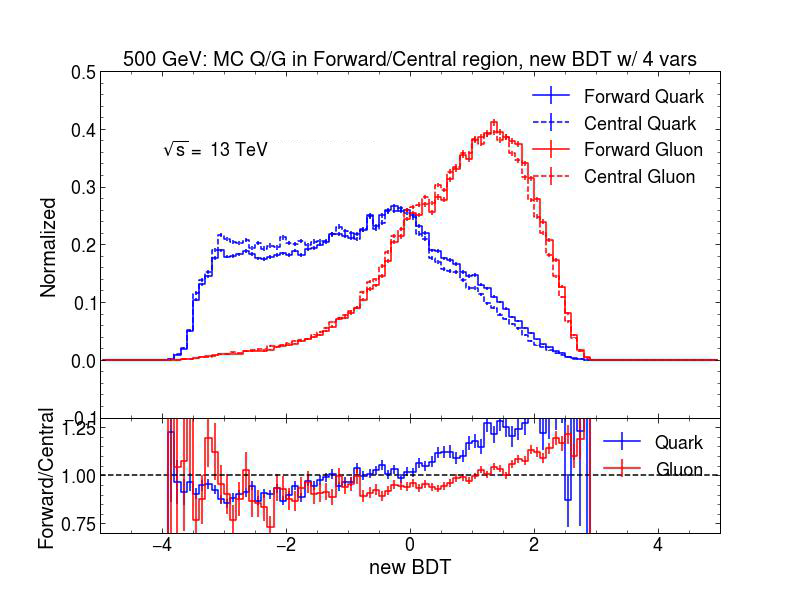
\includegraphics[width=0.45\textwidth]{fig/ADE/new_GBDT/4vars_plots/MC_truth_Q_G_FvsC_500_GBDT_newScore_None.jpg}} \quad
	\subfloat[Training with \abseta, scenario 2]{\label{fig:QG-training-w-eta-500}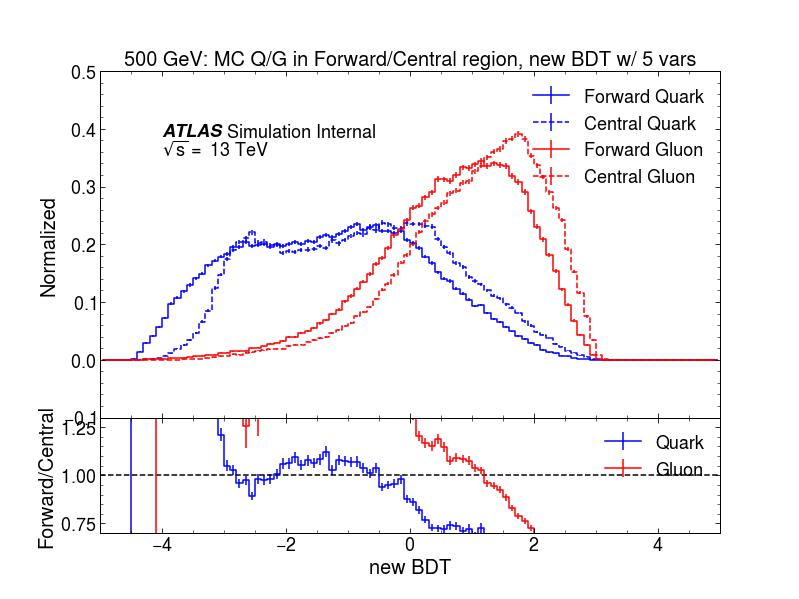
\includegraphics[width=0.45\textwidth]{fig/ADE/new_GBDT/5vars_abseta_plots/MC_truth_Q_G_FvsC_500_GBDT_newScore_None.jpg}}
	\caption[]{
		The comparison of BDT distribution for different scenarios in the jet \pt~range from 500 to 600 GeV. %.
		\label{fig:QG-training_scenario_compare_500_600}
	}
\end{figure}

\paragraph{Training weights}\mbox{}\par
An additional data processing step is conducted to modify the event weights, such that a flat distribution of the \pt~spectrum is given. 
This adjustment is motivated by the observation that higher \pt~jets have less probability to occur, so the training on the higher \pt~jets need to be emphasise. This newly introduced weight, referred to as the "flat \pt-weight" within this context, is exclusively employed during the training process. Conversely, for other scenarios, such as assessing tagger performance on validation datasets and subsequent calibration endeavours, the original event weights based on physical considerations remain employed.

\begin{figure}[htb]
	\centering
	\subfloat[Physical event weight]{\label{fig:QG-training-pt-event-weight}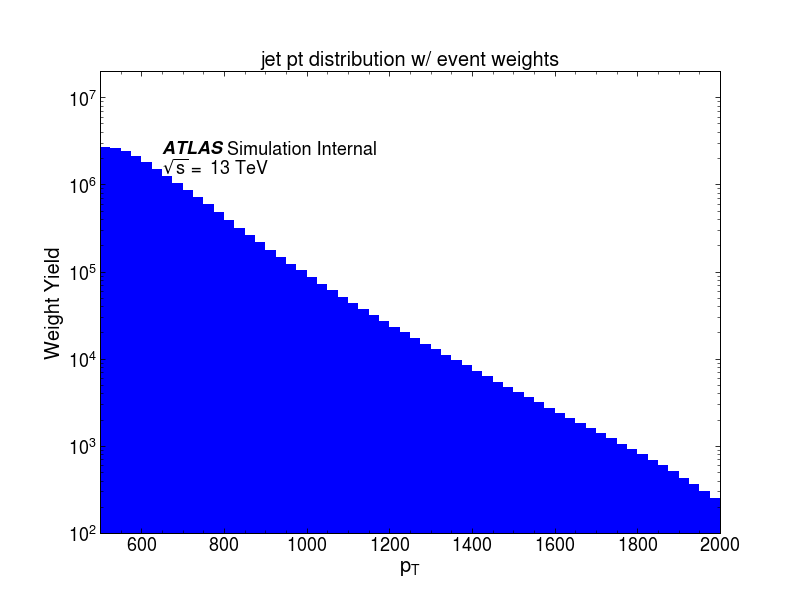
\includegraphics[width=0.45\textwidth]{fig/ADE/new_GBDT/pt_event_weight.png}} \quad
	\subfloat[Flat \pt-weight]{\label{fig:QG-training-pt-flatpt-weight}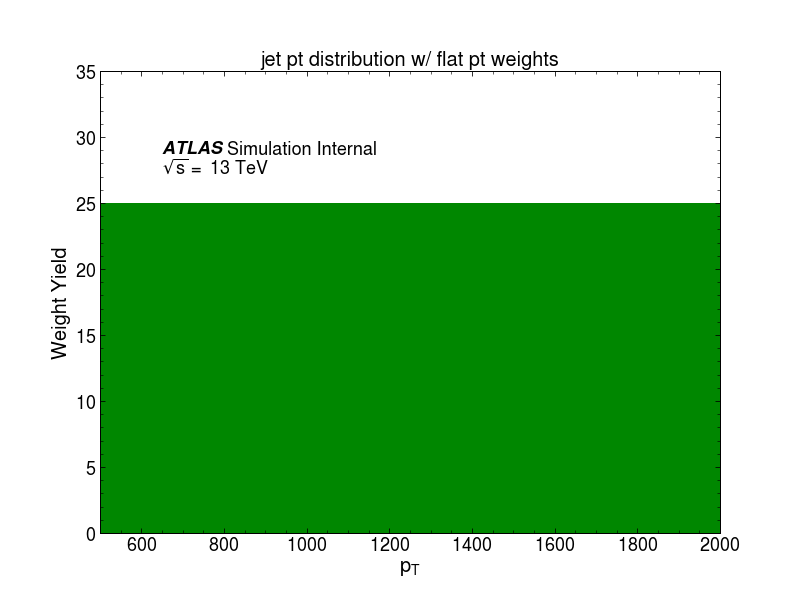
\includegraphics[width=0.45\textwidth]{fig/ADE/new_GBDT/pt_flatpt_weight.png}}
	\caption[]{
		The comparison of jet \pt~distributions with different weights. %.
		\label{fig:QG-training-pt-weight-compare}
	}
\end{figure}

\paragraph{Training Configuration}\mbox{}\par

Approximately 30\% of the data from each period of the MC \pythia8 A, D, E is randomly allocated for the training investigation, constituting an aggregate of roughly 60 million jets. 
The dataset division for training, validation, and testing is structured in a ratio of 80\% for training, 10\% for validation, and 10\% for testing.

Optuna is employed to conduct a search for optimal hyperparameters. Following the hyperparameter tuning process, the most optimal model is achieved after 100 iterations of such procedure. The optimised parameters are listed:

\begin{itemize}
	\item bagging\textunderscore fraction 0.9176347488279626
	\item bagging\textunderscore freq 2
	\item feature\textunderscore fraction 0.9084973008559477
	\item lambda\textunderscore l1 0.0016400096502256838
	\item lambda\textunderscore l0.006327330258011633
	\item min\textunderscore child\textunderscore samples 13
	\item num\textunderscore leaves 224
\end{itemize}

The performance of a classification model at all classification criteria can be illustrated using a receiver operating characteristic (ROC) curve. The idea is to compare the true positive rate (TPR, also known as sensitivity, recall or probability of detection) against the false positive rate (FPR, also known as the probability of false alarm) at different criteria given. Consider a binary classification case, where the outputs are either labelled as positive (p) or negative (n), in total there are four possible outputs from a two-class prediction problem. A true positive (TP) is given if the output from a prediction is p and the actual value is also p, otherwise a false positive (FP) is assigned if the actual value is n. Conversely, a true negative (TN) is given if both the prediction outcome and the actual value are n, whereas a a false negative (FN) is assigned if the actual value is p. TPR as a synonym for recall is defined as:
\begin{equation}
	TPR = TP/(TP+FN)
\end{equation}
while the FPR is defined as: 
\begin{equation}
	FPR = FP/(FP+TN)
\end{equation}

In this analysis, the prediction true is defined by higher \abseta jet and prediction negative is defined by lower \abseta jet. The actual truth value is given by the quark jet from the MC truth information, whereas the actual negative value is given by the gluon truth information. Thus the quark efficiency is the TPR and the gluon rejection is FPR. An Area Under the ROC Curve (AUC) is used to evaluate the performance of a classifier, the better performance is indicated by higher AUC values.

Several ROC plots are made to compare different features and the BDT in different \pt~ranges. 
To check whether the BDT tagger is overtrained, the shape comparison is shown in Figure~\ref{fig:overtraining-validation}, between training dataset and validation dataset.  
No overtraining is observed as the distribution of training dataset is very similar to that of testing dataset. 

Figure~\ref{fig:QG-ROC_500_600} shows the ROC curve for all single jet variables and the BDT-tagger in given \pt~ranges in forward and central regions. Figure~\ref{fig:QG-ROC_800_1000}  shows the AUC of both \ntrk-only tagger and the BDT-tagger as a function of jet \pt. 
\begin{figure}[h]
	\centering
	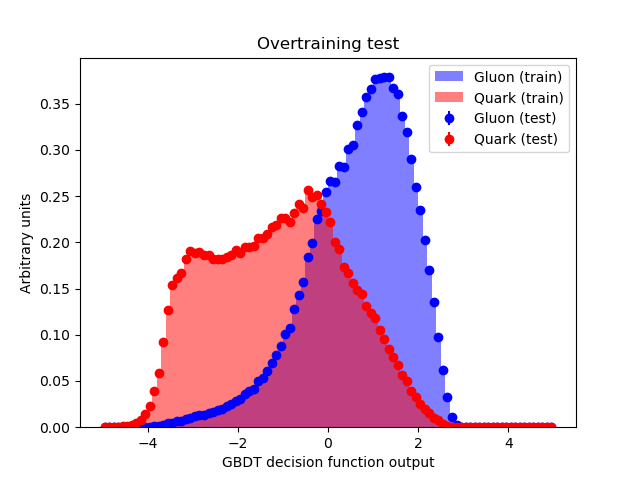
\includegraphics[width=0.65\textwidth]{fig/ADE/new_GBDT/4vars_plots/overtrain_validation.png}
	\caption{Overtraining validation}
	\label{fig:overtraining-validation}
\end{figure}

\begin{figure}[htb]
	\centering
	\subfloat[Forward region ]{\label{fig:QG-NtrkDataMCinclPythiaa}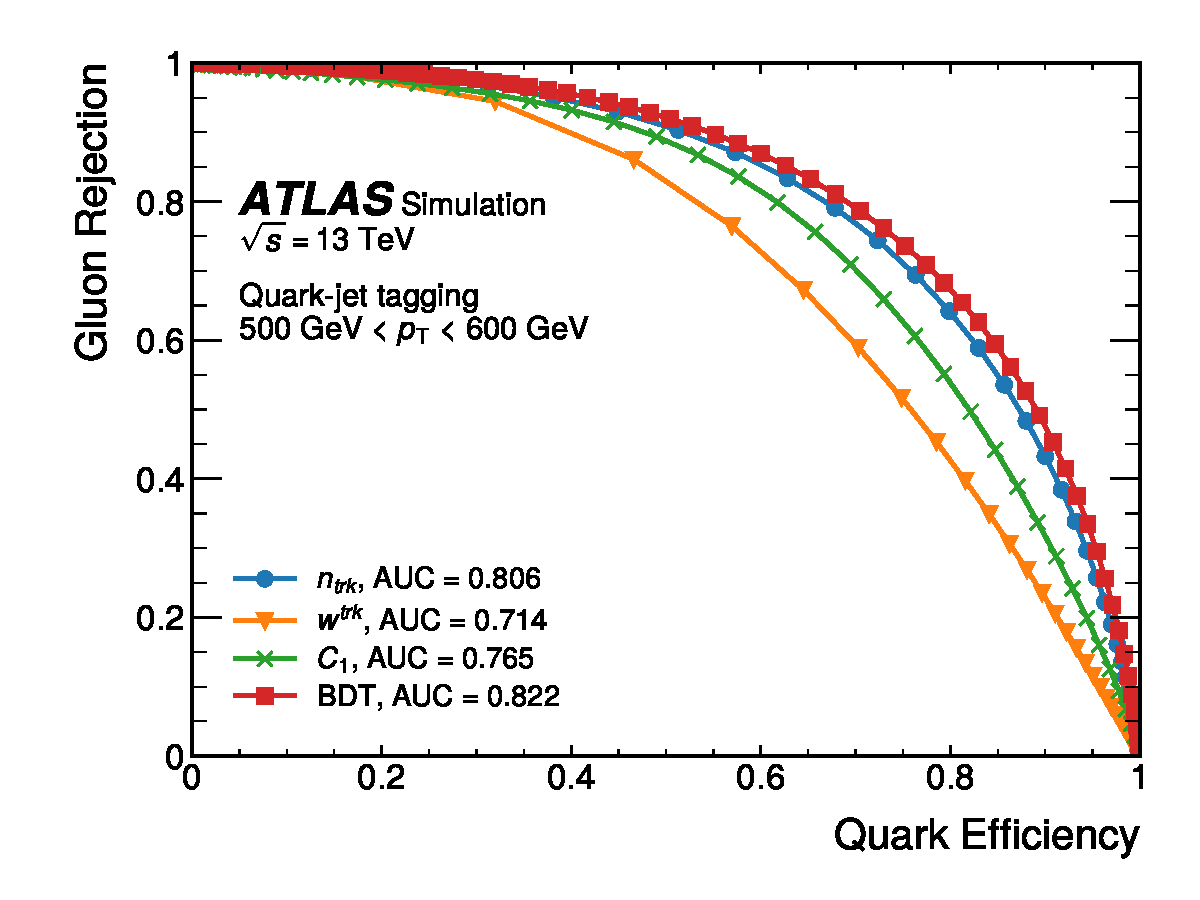
\includegraphics[width=0.48\textwidth]{fig/ROC/ROC_500_Forward_none.pdf}} \quad
	\subfloat[Central region ]{\label{fig:QG-NtrkDataMCinclPythiab}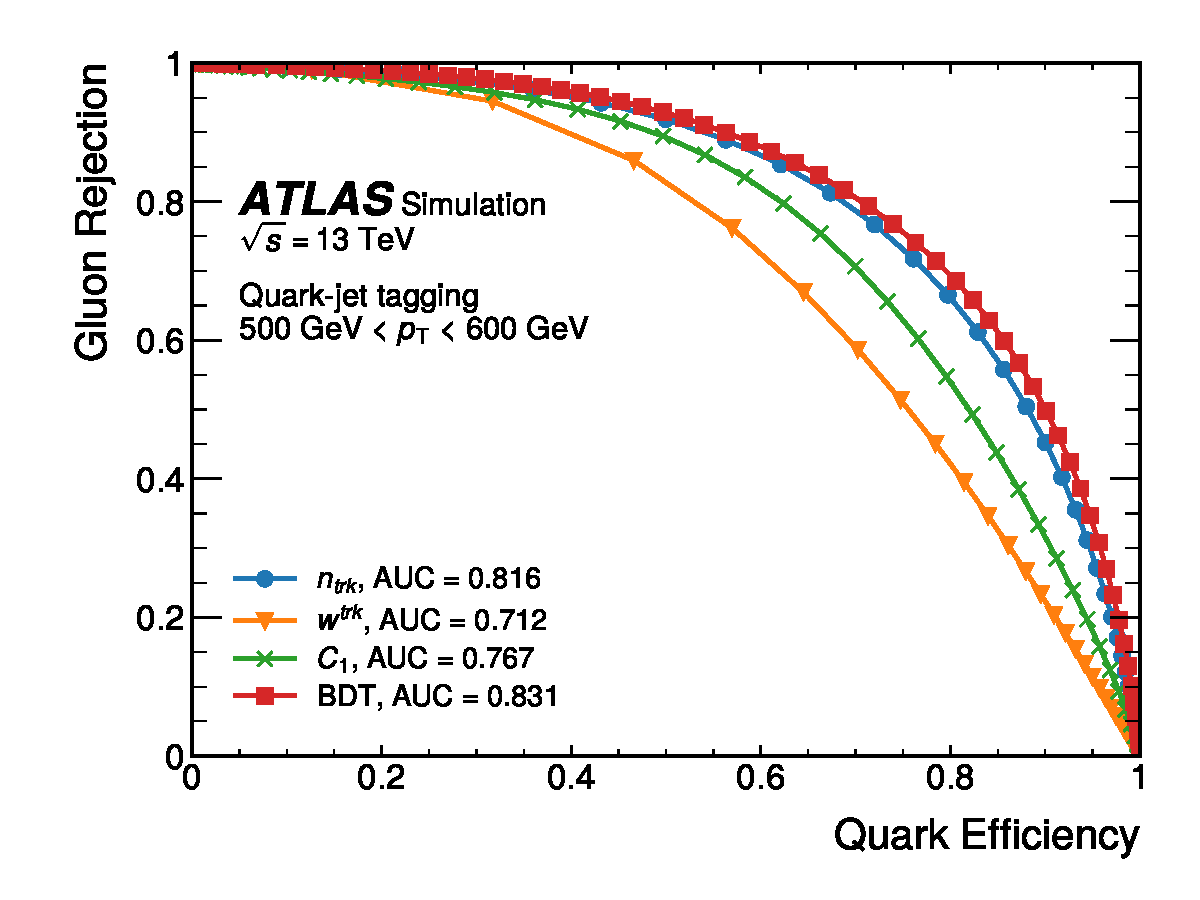
\includegraphics[width=0.48\textwidth]{fig/ROC/ROC_500_Central_none.pdf}}
	\caption[]{
		The ROC Curve for different taggers in the given jet \pt. %.
		\label{fig:QG-ROC_500_600}
	}
\end{figure}


\begin{figure}[htb]
	\centering
	\subfloat[Forward region ]{\label{fig:QG-NtrkDataMCinclPythiaa}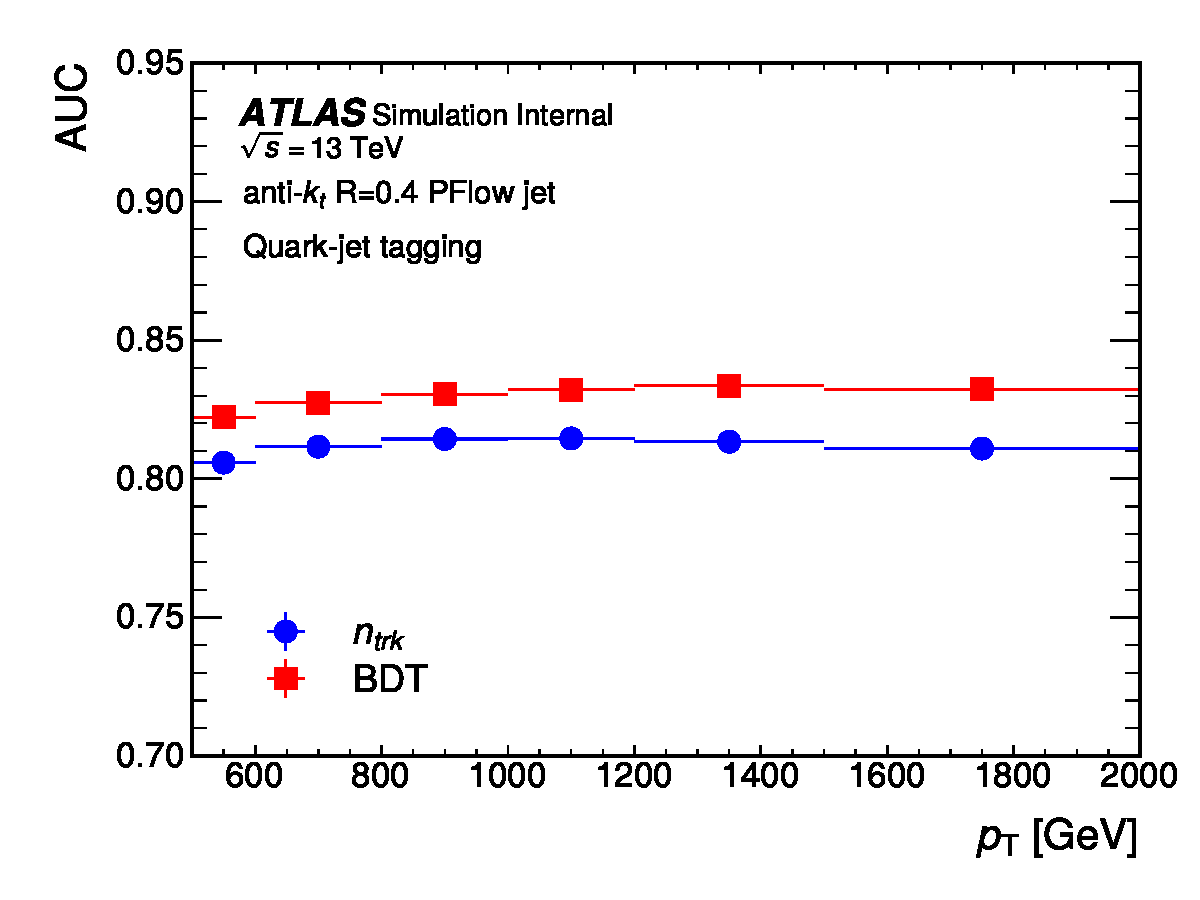
\includegraphics[width=0.48\textwidth]{fig/ROC/pt_Forward_GBDT_newScore.pdf}} \quad
	\subfloat[Central region]{\label{fig:QG-NtrkDataMCinclPythiab}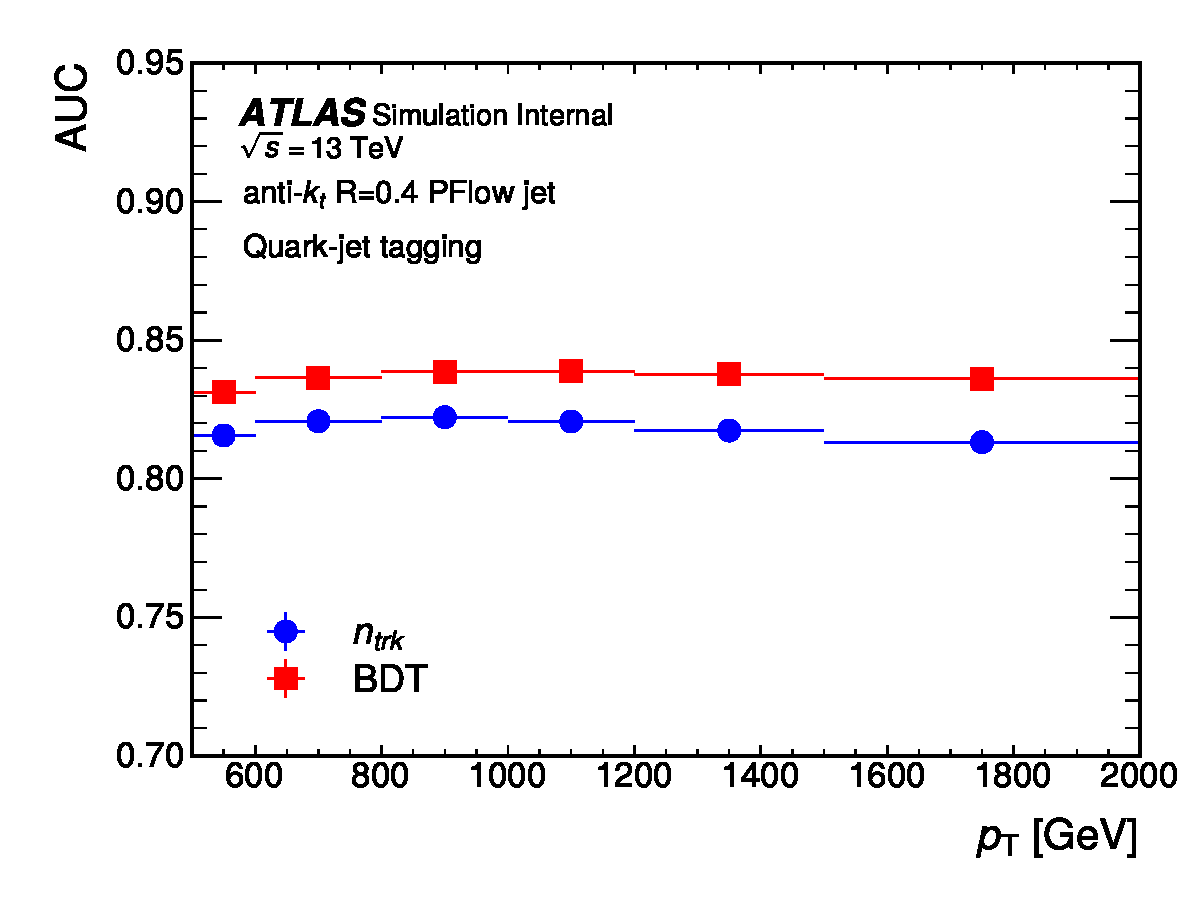
\includegraphics[width=0.48\textwidth]{fig/ROC/pt_Central_GBDT_newScore.pdf}}
	\caption[]{
		The AUC for different taggers across jet \pt. %.
		\label{fig:QG-ROC_800_1000}
	}
\end{figure}

%A receiver operating characteristic (ROC) curve,  is a graph showing the performance of a classification model at all classification thresholds. The ROC curve is created by plotting the true positive rate (TPR) against the false positive rate (FPR) at various threshold settings. The true-positive rate is also known as sensitivity, recall or probability of detection. The false-positive rate is also known as the probability of false alarm and can be calculated as (1-specificity).
%
%Consider a two-class prediction problem (binary classification), in which the outcomes are labeled either as positive (p) or negative (n). There are four possible outcomes from a binary classifier. If the outcome from a prediction is p and the actual value is also p, then it is called a true positive (TP); however, if the actual value is n then it is said to be a false positive (FP). Conversely, a true negative (TN) has occurred when both the prediction outcome and the actual value are n, and a false negative (FN) is when the prediction outcome is n while the actual value is p.
%
%TPR is a synonym for recall and is therefore defined as follows: TPR $=$ TP/(TP+FN), while the FPR is defined as follows: FPR $=$ FP/(FP+TN). In this analysis,  \abseta jet is defined as the prediction true and central \abseta jet is defined as the prediction negative, the truth quark-jet from MC simulation is defined as the actual truth value, the gluon-jet is defined as the actual negative value. Thus, the TPR is quark efficiency and FPR is gluon rejection.

%In classification problems, Area Under the ROC Curve(AUC) is used to evluate the classifier performance. The forward AUC values indicate better performance. The AUC are shown in the ROC plots along the legends. 

The \ntrk-only tagger is found to be the most sensitive observable than other individual jet substructure variables for $q/g$ tagging, 
\wtrk~and \cbeta~are less sensitive to the number of tracks inefficiencies because they are defined as ratios, the BDT-tagger which include the $\wtrk$ and $\cbeta$ has better AUC than \ntrk-only tagger across all jet \pt~ranges. This indicates that the BDT-based tagging mechanism has a heightened capacity to discriminate against gluon-jets at the same level of efficiency in identifying quark-jets with \ntrk-only tagger . Both taggers are calibrated in this paper, more details are presented in the next section.

%\wtrk and \cbeta are less sensitive to the number of trackstrack inefficiencies because they are defined as ratios. %only and it has only a small \eta dependency. %
%\texttt{TightPrimary} identified tracks have few fake tracks and only a small \eta dependency. %

%since such a jet substructure information is not used in the conventional SUSY searches and %
%the mis-modeling of the simulation, especially in a gluon, is known in the previous study for q/g tagging in Run1~\cite{QGRun1}. %

\FloatBarrier



\subsection{Matrix Method}
\label{sec:QG-method}
The distribution of q/g tagging variables depend strongly on jet \pt. Thus a matrix method~\cite{ATL-PHYS-PUB-2017-009} approach used to extract the shape of the $q/g$ tagging variables is performed on each \pt~bin defined in Table~\ref{tab:QG-ptbinning} for quark- and gluon-jets, separately. 

\begin{table}[hptb]
\centering
\begin{tabular}{|c|c|c|c|c|c|}
 \hline
 \multicolumn{6}{|c|}{\pt~bin boundary [GeV] } \\ \hline
   500-600 & 600-800 & 800-1000 & 1000-1200 & 1200-1500 & 1500-2000  \\ \hline
  \multicolumn{6}{|c|}{\multirow{2}{*}{Forward \& Central \abseta jet samples in multi-jet}} \\ 
  \multicolumn{6}{|c|}{} \\ \hline
\end{tabular}
\caption{
	The \pt~range division for the calibration of the $q/g$ tagging variables and samples used in extraction of pure quark and gluon jets. %
}
\label{tab:QG-ptbinning}
\end{table}

To measure the performance of the $q/g$ taggers under study, samples exclusively composed of either quark-jets or gluon-jets are needed. In order to deduce the distribution shapes of the $q/g$ tagging variables pertaining to quark- and gluon-jets within the empirical data, a methodology that capitalizes on samples possessing varying q/g ratios is employed. This approach, known as the matrix method~\cite{ATL-PHYS-PUB-2017-009}, facilitates the extraction of the distinct distributions of $q/g$ tagging variables for the aforementioned jet categories.

Pure quark- or gluon-jets can be extracted from forward and central jet samples following the matrix: 
\begin{eqnarray}
	\label{eq:QG-matrix2}
	\left(\begin{array}{c} 
		p_{\mrm{F}}(x)\\ 
		p_{\mrm{C}}(x)\\ 
	\end{array}\right)
	&=&
	\underbrace{
		\left(\begin{array}{cc}
			f_{\mrm{F,Q}}&f_{\mrm{F,G}}\\
			f_{\mrm{C,Q}}&f_{\mrm{C,G}}\\
		\end{array}\right)
	}_{\scalebox{1}{$\equiv F$}}
	\left(\begin{array}{c} 
		p_\mrm{Q}(x)\\ 
		p_\mrm{G}(x)\\ 
	\end{array}\right)
	\\
	\label{eq:QG-invmatrix2}
	%\Leftrightarrow
	\left(\begin{array}{c} 
		p_\mrm{Q}(x)\\ 
		p_\mrm{G}(x)\\ 
	\end{array}\right)
	&=& F^{-1}
	\left(\begin{array}{c} 
		p_{\mrm{F}}(x)\\ 
		p_{\mrm{C}}(x)\\ 
	\end{array}\right).
\end{eqnarray}


where $p_{\mrm{Q,G}}(x)$ represents the distributions of the $q/g$ tagging variable $x$ in pure quark- and gluon-enriched jet samples, 
$p_{\mrm{F}}(x)$ and $p_{\mrm{C}}(x)$ show the distributions of jet variables in forward and central regions, respectively, $f_{\mrm{F/C},\mrm{Q/G}}$ are the fractions of quarks and gluons in a forward or central region. %
The inverse matrix of $F$ is thus constructed and used to extract pure quark/gluon~$p_{\mrm{Q,G}}$. %
Data is used to obtain the distributions of the quark- and gluon-enriched samples, MC is used to calculate the fraction of quarks and gluons in them as shown in Figure~\ref{fig:QG-Fmc}, as well as the distributions of $q/g$ tagging variables. %
The matrix is calculated in each $x$ bin and each jet \pt~range.


\begin{figure}[htb]
	\centering
	\subfloat[]{\label{fig:QG-Fmcd}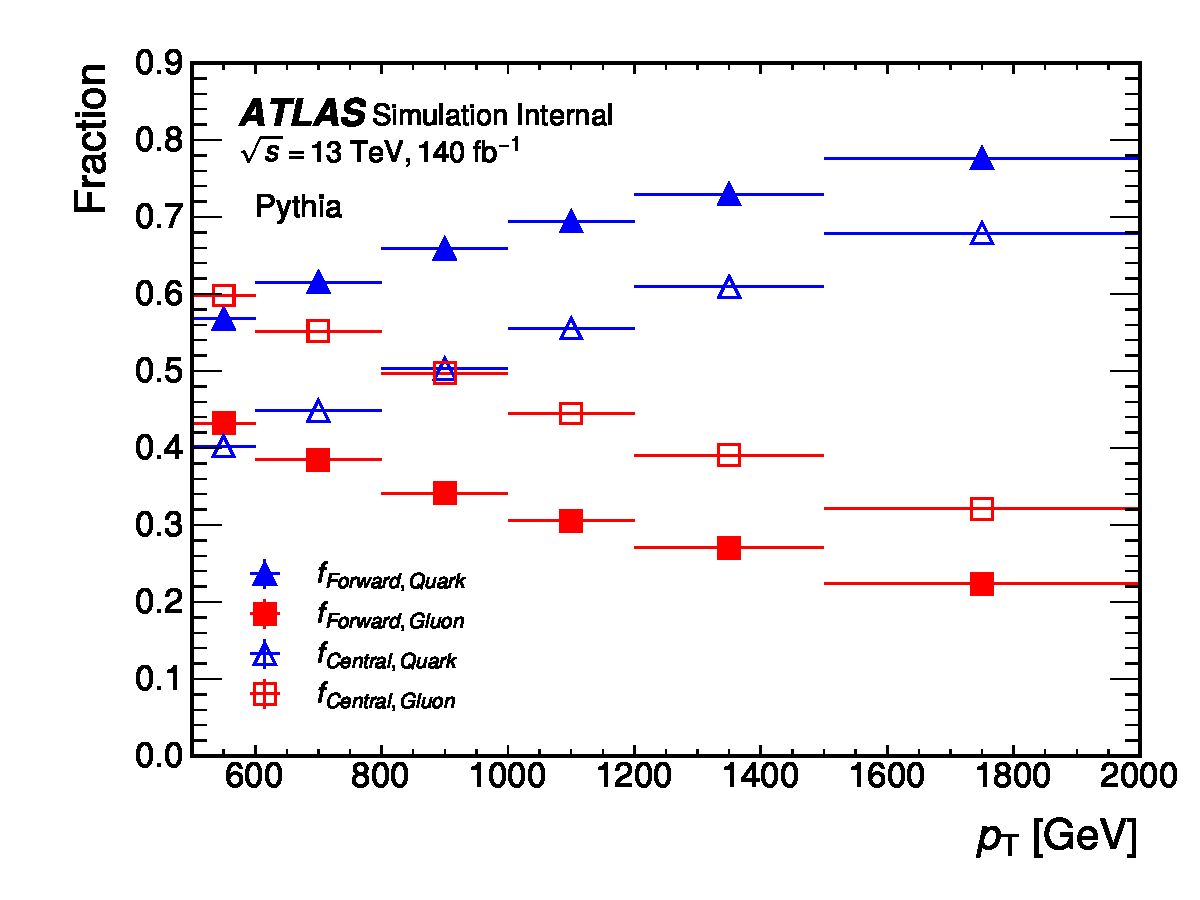
\includegraphics[width=0.6\textwidth]{fig/ADE/frac/Fraction_jet_nTracks_pythia.pdf}}\quad
	\caption[]{
		Fractions of quark-jets and gluon-jets  %
		in forward jet and central jet regions from {\pythia} dijet process. These values are used as elements in $F$ matrix in Equation \ref{eq:QG-matrix2}. %
		\label{fig:QG-Fmc}
	}
\end{figure}

\begin{figure}[htb]
	\centering
	\subfloat[Forward region ]{\label{fig:QG-Quark-Fraction-forward}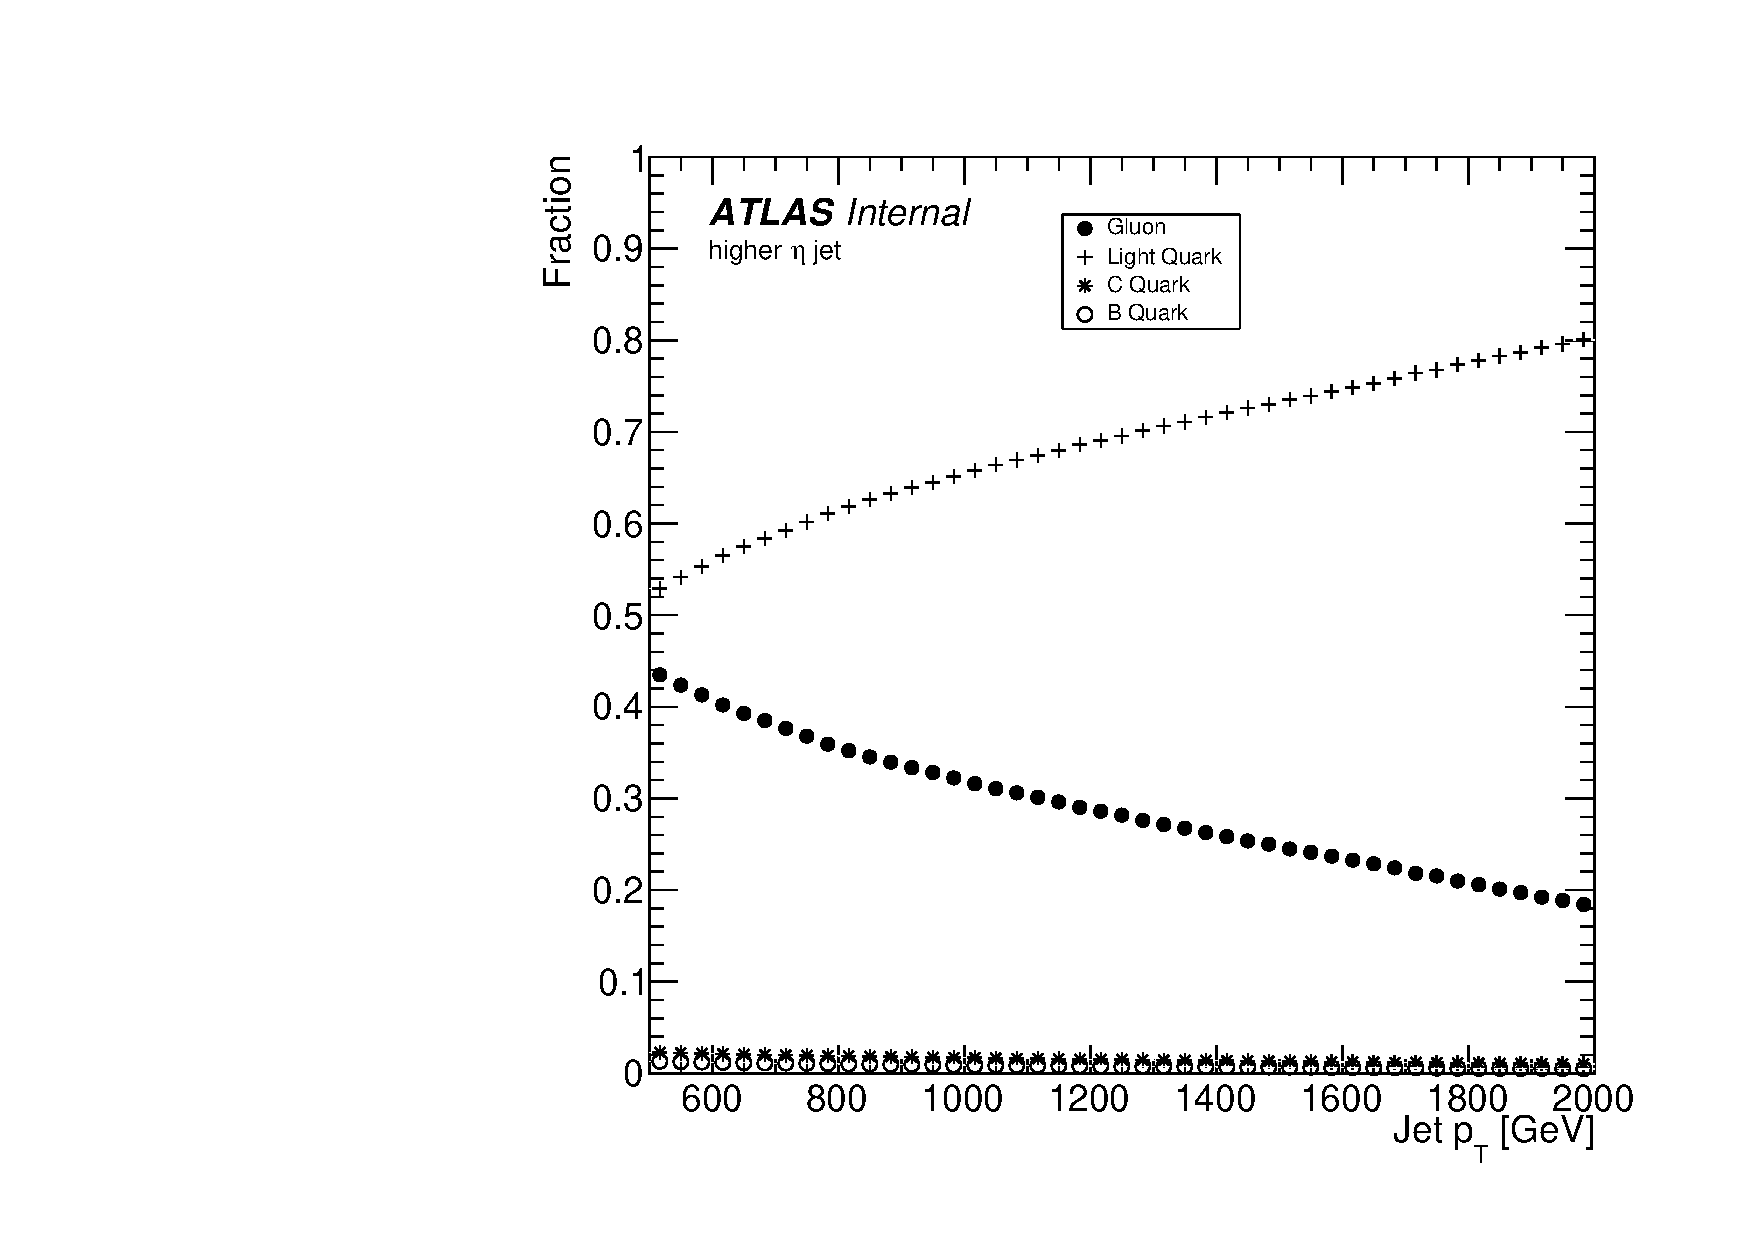
\includegraphics[width=0.45\textwidth]{fig/ADE/higher_fraction.pdf}} \quad
	\subfloat[Central region ]{\label{fig:QG-Quark-Fraction-central}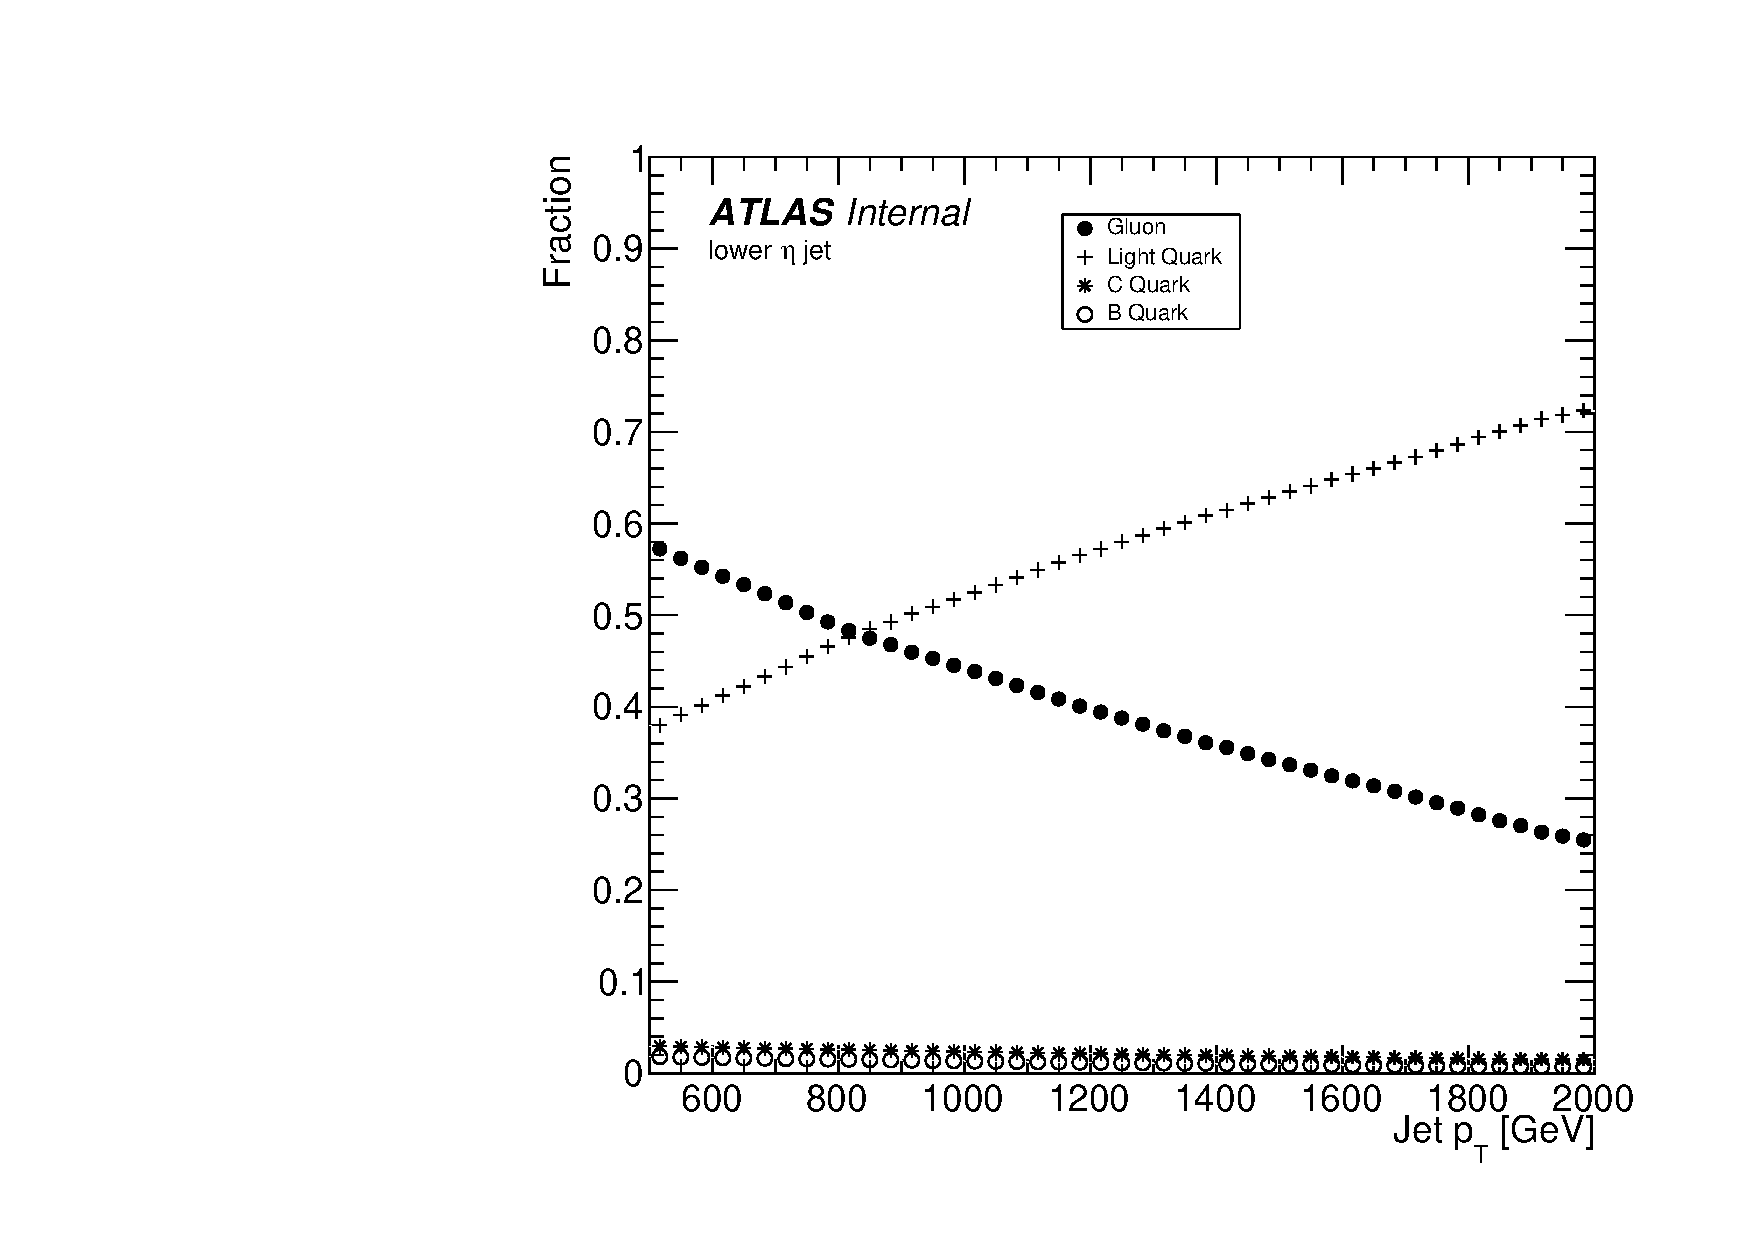
\includegraphics[width=0.45\textwidth]{fig/ADE/lower_fraction.pdf}} \quad
	\caption[]{
		Flavor composition of of forward \subref{fig:QG-Quark-Fraction-forward}  or central  \subref{fig:QG-Quark-Fraction-central} multi-jet events. %.
		\label{fig:QG-quark-fraction}
	}
\end{figure}


Figure~\ref{fig:QG-quark-fraction} illustrates the fraction of light and heavy quark- and gluon-jets in the \pythia8 dijet sample. These fractions are depicted in a stacked format, summing up to a cumulative value of 1. It should be noted that the involvement of heavy flavour quarks constitutes a minor fraction, amounting to a few percent, and is deemed negligible for the later study.
Previous investigations~\cite{ref21} have established that any discrepancies among the fractions derived from various MC event generators remain minimal. Furthermore, the shapes of distributions obtained from the MC simulations generally exhibit congruence with those observed within the  data.
The distributions of \ntrk~and BDT score in higher and lower jet regions are shown in Figure~\ref{fig:QG-ntrk-method1} and Figure~\ref{fig:QG-jetHLPt} in jet \pt~range 500 GeV - 600 GeV. The shapes of distributions obtained from the MC simulations is generally consistent with that from data.

\begin{figure}[htb]
	\centering
	\subfloat[Forward region]{\label{fig:QG-jetHLPta}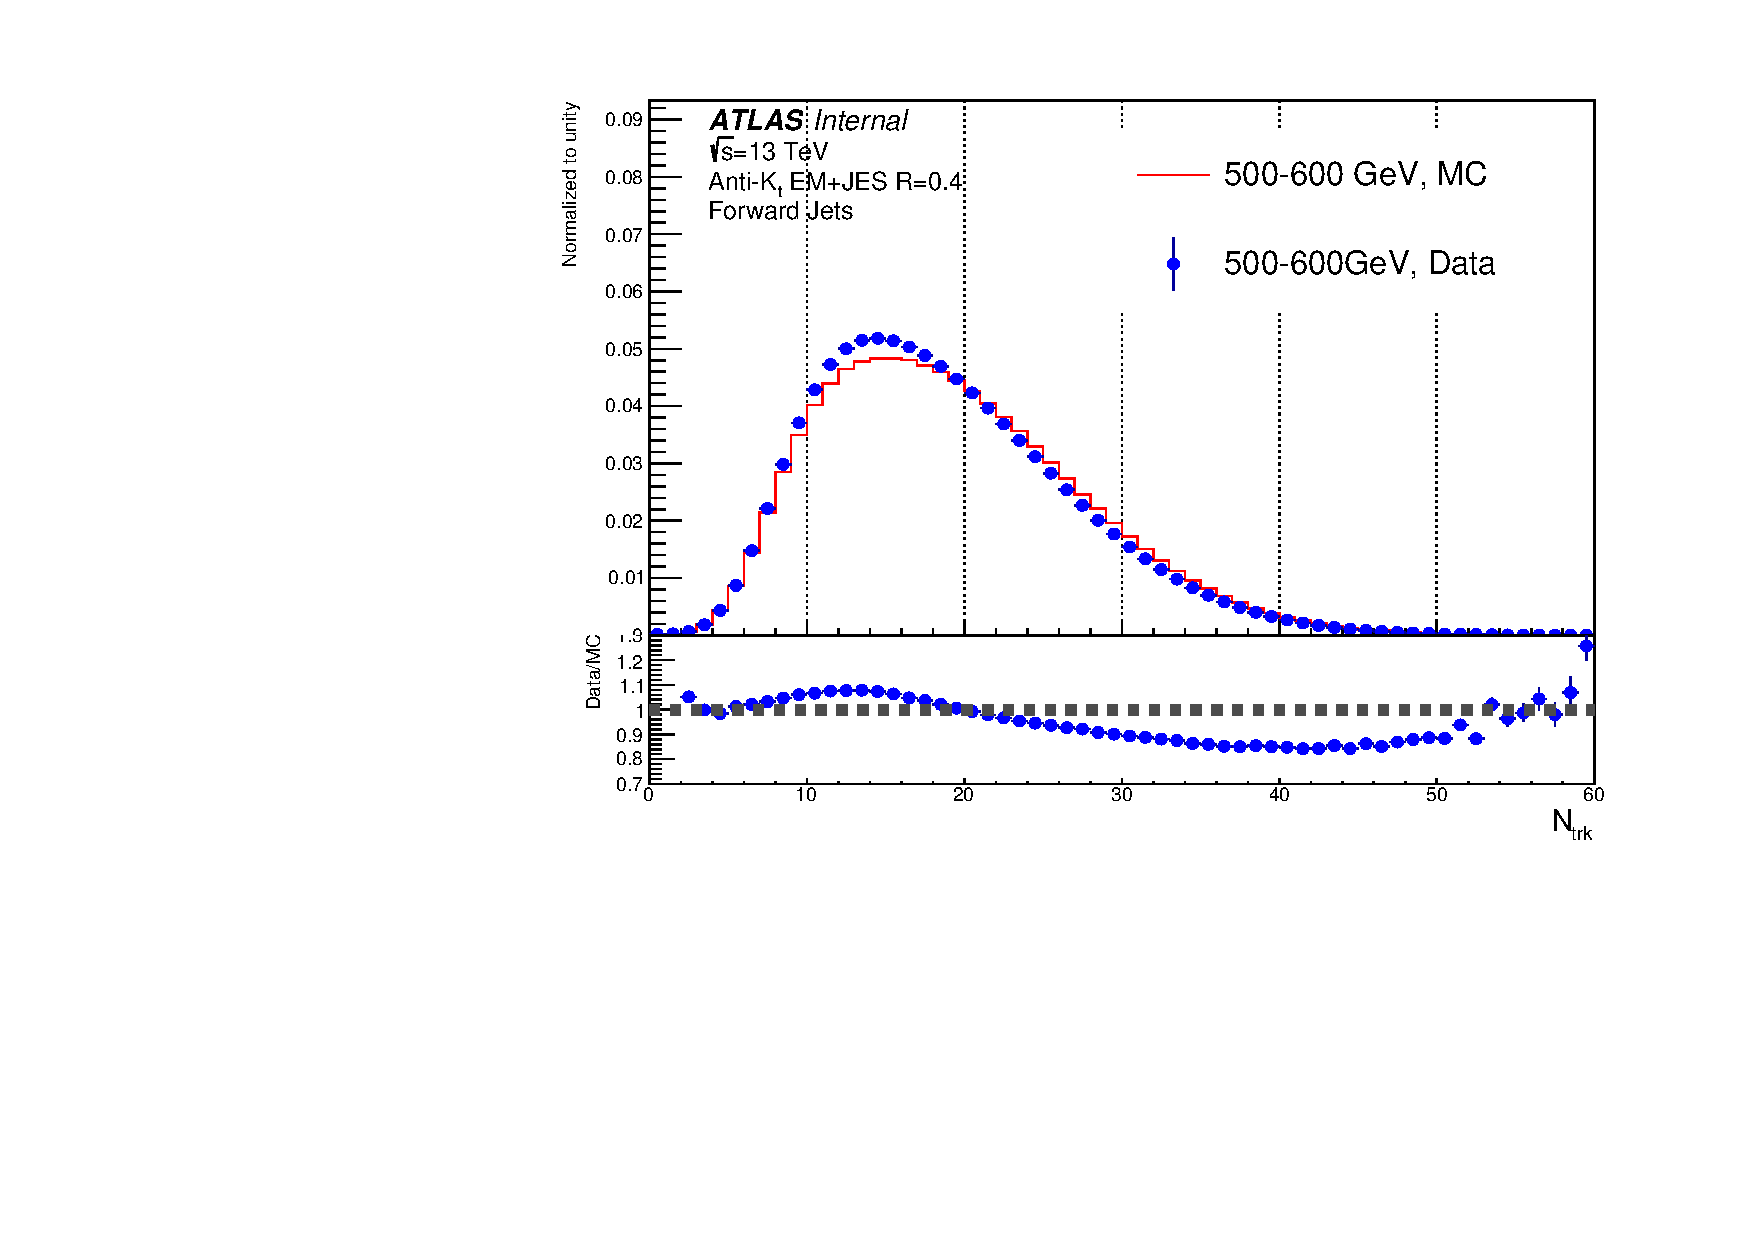
\includegraphics[width=0.45\textwidth]{fig/dijetanalysis/pythia-nominal/kinematics/ntrk_Forward_500_600_Pythia.pdf}} \quad
	\subfloat[Central region ]{\label{fig:QG-jetHLPtb}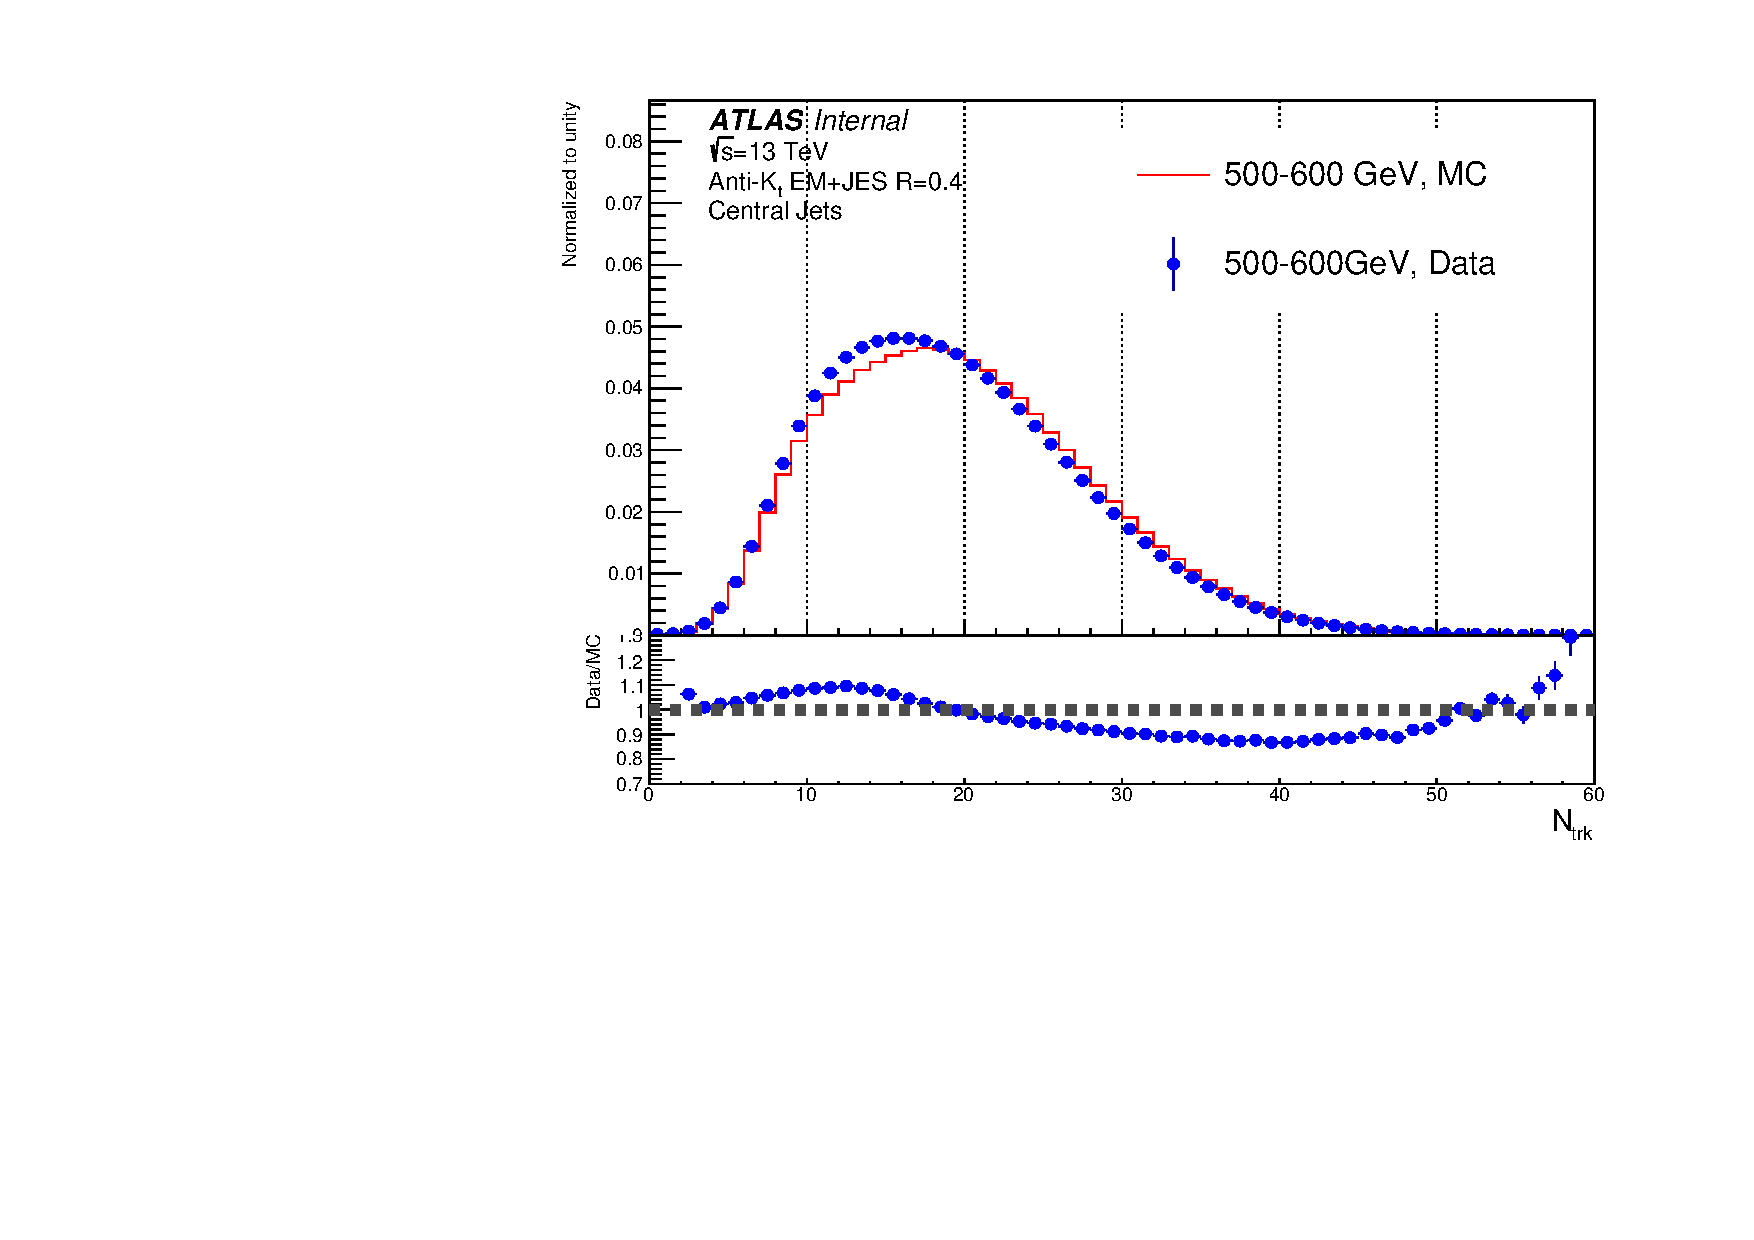
\includegraphics[width=0.45\textwidth]{fig/dijetanalysis/pythia-nominal/kinematics/ntrk_Central_500_600_Pythia.pdf}}\\
	\caption[]{
	  The \ntrk~distribution of the leading two jets with {\pythia8} in the MC and data.
		\label{fig:QG-ntrk-method1}
	}
\end{figure}

\begin{figure}[htb]
	\centering
	\subfloat[Forward region]{\label{fig:QG-jetHLPta}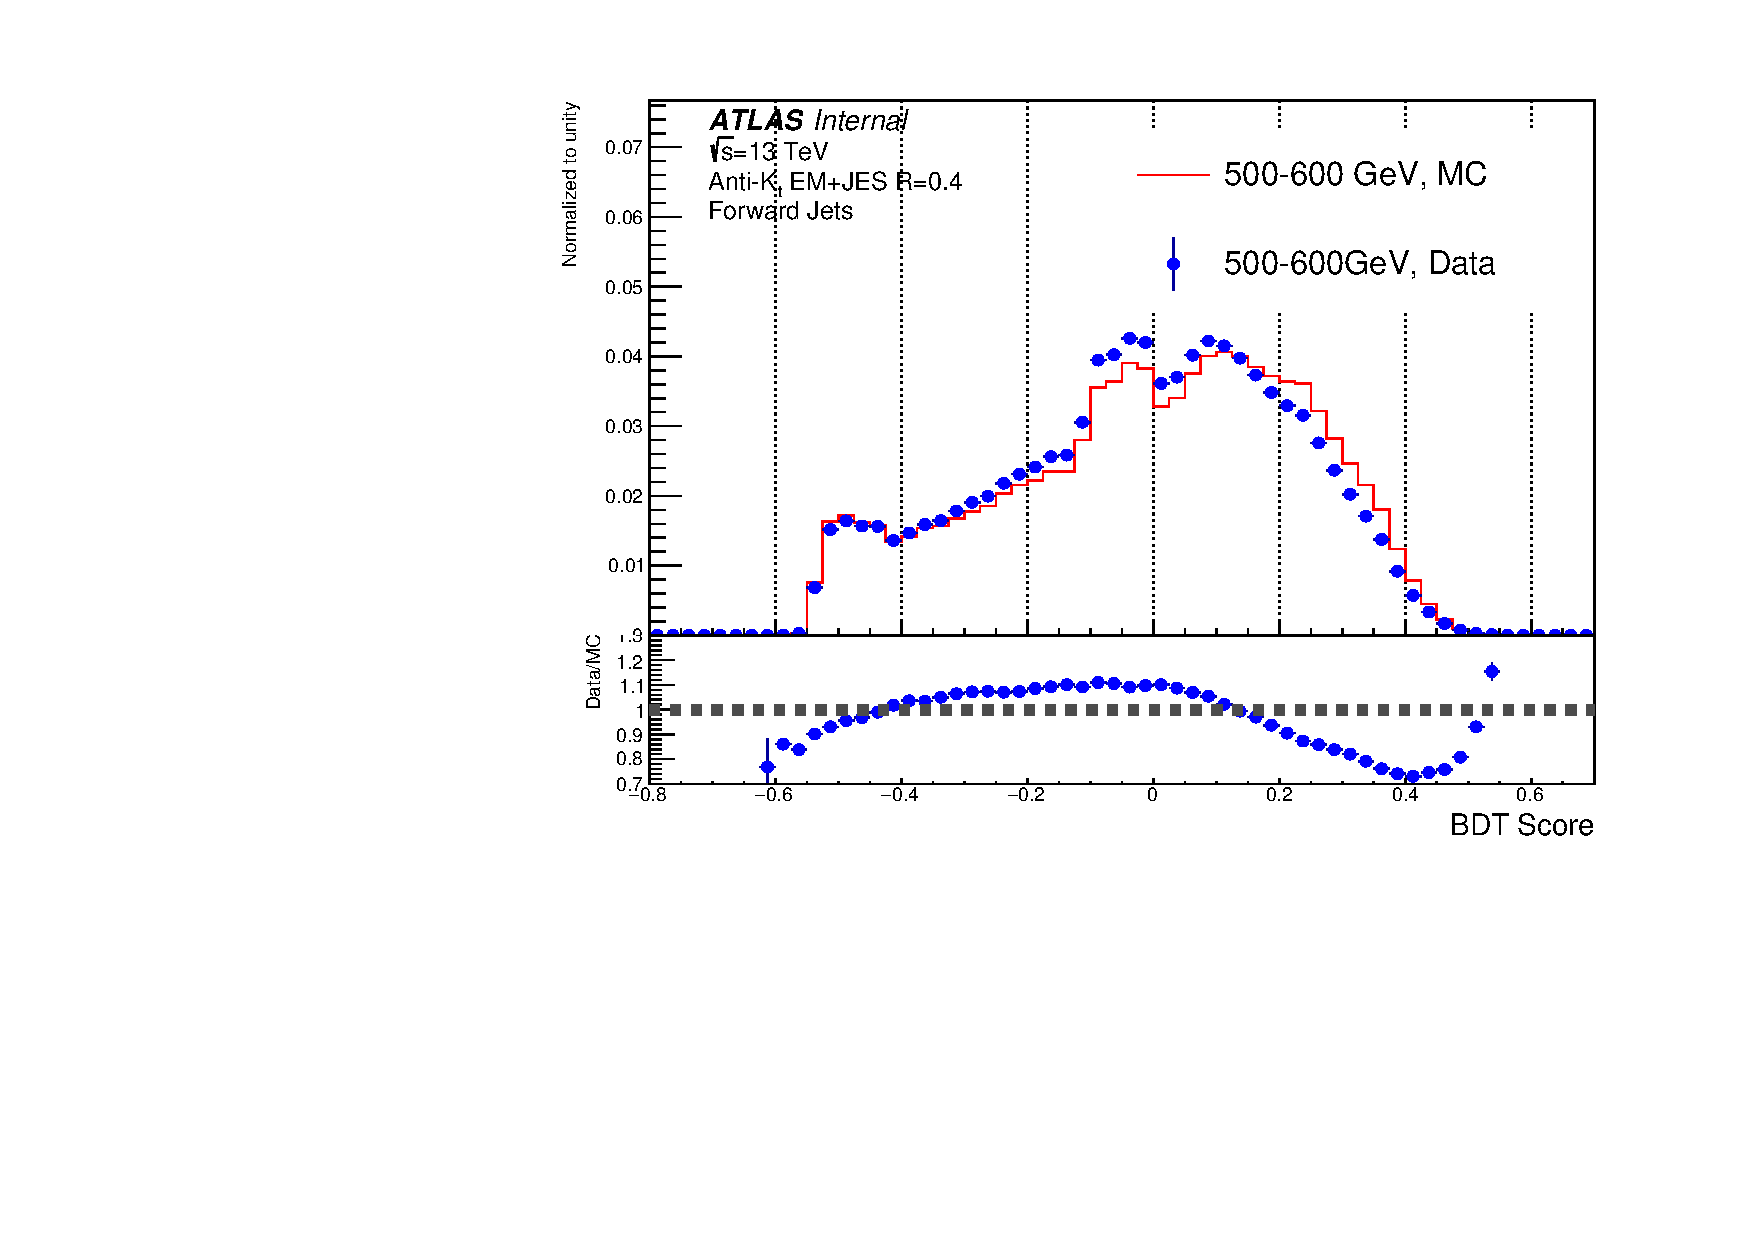
\includegraphics[width=0.45\textwidth]{fig/dijetanalysis/pythia-nominal/kinematics/bdt_Forward_500_600_Pythia.pdf}} \quad
	\subfloat[Central region ]{\label{fig:QG-jetHLPtb}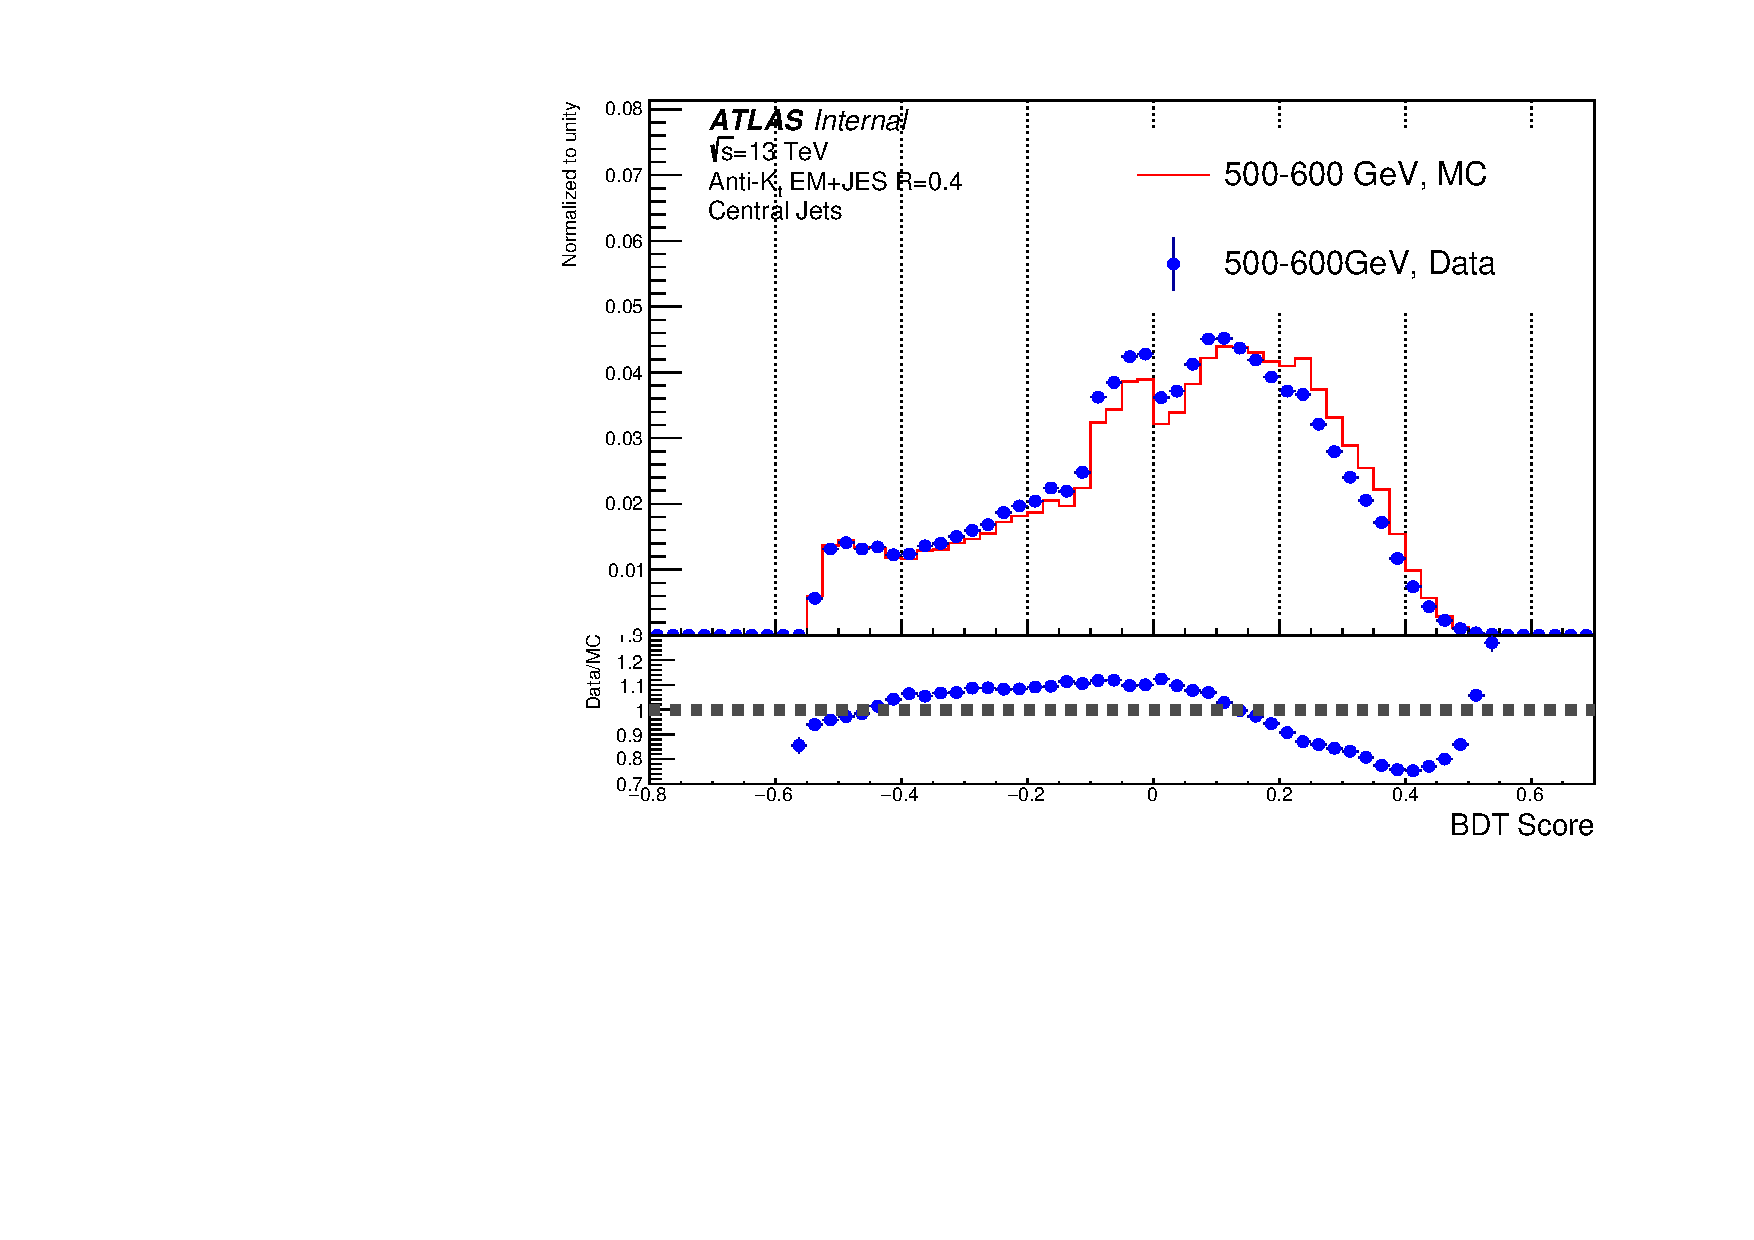
\includegraphics[width=0.45\textwidth]{fig/dijetanalysis/pythia-nominal/kinematics/bdt_Central_500_600_Pythia.pdf}}\\
	\caption[]{
	  The BDT score distribution of the leading two jets with {\pythia8} in the MC and data.
	    %Data for four plots are 139\ifb in total.	The normalization of the simulation is decided by cross-section.
		\label{fig:QG-jetHLPt}
	}
\end{figure}



%The matrix in 2-process extraction is given as 
%\begin{eqnarray}
%\label{eq:QG-matrix}
%\left(\begin{array}{c} 
%p_{\mrm{$\gamma$+jets}}(x)\\ 
%p_{\mrm{Multi-jet}}(x)\\ 
%\end{array}\right)
%&=&
%\underbrace{
%	\left(\begin{array}{cc}
%	f_{\mrm{$\gamma$+jets,Q}}&f_{\mrm{$\gamma$+jets,G}}\\
%	f_{\mrm{Multi-jet,Q}}&f_{\mrm{Multi-jet,G}}\\
%	\end{array}\right)
%}_{\scalebox{1}{$\equiv F$}}
%\left(\begin{array}{c} 
%p_\mrm{Q}(x)\\ 
%p_\mrm{G}(x)\\ 
%\end{array}\right)
%\\
%\label{eq:QG-invmatrix}
%\Leftrightarrow
%\left(\begin{array}{c} 
%p_\mrm{Q}(x)\\ 
%p_\mrm{G}(x)\\ 
%\end{array}\right)
%&=& F^{-1}
%\left(\begin{array}{c} 
%p_{\mrm{$\gamma$+jets}}(x)\\ 
%p_{\mrm{Multi-jet}}(x)\\ 
%\end{array}\right),
%\end{eqnarray}




%To estimate the systematic uncertainty coming from the parton shower modeling, %
%this calibration is performed for \pythia8 and \sherpa~separately. %
%%For \pythia8, both of the $Z$+jets and multi-jet MCs are \pythia8. %
%%For \sherpa, the $Z$+jets MC is \sherpa2.2.1 and the multi-jet MC is \sherpa2.1.1. %
%%This difference will be taken into account in the systematic uncertainties. %
%In \Sectrange{sec:QG-method}{sec:QG-SF}, the figures using \pythia8~(\sherpa) show results %
%with  NNPDF30~(NNPDF30) and NNPDF23LO~(CT10) PDF sets for 2-process extraction and for higher/lower \abseta jet extraction, respectively. %

%In \Sectrange{sec:QG-var}{sec:QG-SF}, the figures show the result with the \pythia8 parton shower modeling
%and the NNPDF30 PDF set for 2-process extraction or NNPDF23LO set for higher/lower \abseta jet. %
%A14 tuned NNPDF23LO set. %




%\begin{tabular}{l|l|c|c|cc}
% \hline
% \multicolumn{2}{l|}{\multirow{3}{*}{Selection}}& \multirow{3}{*}{$\gamma$+jets sample} & \multicolumn{3}{c}{Multi-jet sample}  \\ 
% \hhline{~~~---}
% \multicolumn{2}{l|}{} &                        & For 2-process & Higher |\etaX| & Lower |\etaX| \\ 
% \multicolumn{2}{l|}{} &                        & extraction    & jet sample  & jet sample \\ \hline 
% & Trigger   & Single photon trigger & \multicolumn{3}{c}{Or of single jet triggers} \\ 
% & MC-specialized cut & - & \multicolumn{3}{c}{$0.5<p_{\mrm{T,avg}}(\mrm{jets})/p_{\mrm{T,truth}}(j_1)<1.5$} \\ 
% & Number of jets        &  $\geq1$ & \multicolumn{3}{c}{$\geq2$} \\ \hhline{~~~---}
%  & $\pt$($\gamma$)             & $>125$     &-   & \multicolumn{2}{c}{-}   \\ 
% & $\pt(j_1)$             & $>50$     &$>50$  &\multicolumn{2}{c}{$>500$} \\ 
%  & $\pt(j_1)/\pt(j_2)$   &  -       & -    & \multicolumn{2}{c}{$<1.5$} \\ 
% & $|\eta(j_1)|$         &  $<2.1$  & $<2.1$ & \multicolumn{2}{c}{$<2.1$}   \\ 
% & $|\eta(j_2)|$         &  -       & -      & \multicolumn{2}{c}{$<2.1$}   \\ \hline
% & Target parton         &  Quark   & Gluon  & Quark  & Gluon       \\ \hhline{~-----}
% & Used jet in $j_1$ or $j_2$ & Only $j_1$ & Only $j_1$ & Higher $|\etaX|$ jet & Lower $|\etaX|$ jet \\
% \hline
%\end{tabular}

%In a low \pt range~($<500\GeV$), the quark fraction of  $\gamma$+jets is high~($\sim75\%$) %
%and the difference between the quark fractions in  $\gamma$+jets and multi-jet is large~($30$--$50\%$), %
%but the quark fraction of higher \abseta jet is low~($\lesssim 50\%$). % 
%Thus, the $\gamma$+jets and multi-jet are used as quark/gluon-enriched samples in the low \pt range. %
%In a high \pt range~($>500\GeVX$), higher \abseta jet has a large fraction of quarks~($>60\%$). %
%Thus, in the low \pt range, the higher/lower \abseta jet samples are used\footnote{
%The low statistics of $\gamma$+jets sample in the higher \pt range is another reason to use the higher/lower \abseta jet samples. %
%}. %
%The fractions are obtained from \pythia8 and \sherpa, separately. %


%\subsection{Method 1 for high \pt jet}
%\label{sec:method1_intro}

%\subsubsection{Background study}
%{\textcolor{red}{Wanyun: please add the background study here and tell people the background for dijet is negiligible}}
%In the whole \pt range, b-quark jets and jets labeled "other" exist, but it is suppressed to be lower than a few \%, which can be ignored. The jets labeled "other" are jets mainly originating from pileup.


%\FloatBarrier

% Data v.s. MC comparison in inclusive gamma+jets or Multi-jet(2sample ext.)

%\begin{figure}[htb]
%	\centering
%	\subfloat[$100<\pt<150\GeV$~(\sherpa) ]{\label{fig:QG-NtrkDataMCinclSherpaa}\includegraphics[width=0.45\textwidth]{Figures/dijetgammajetanalysis/MC_Closure/dist_comparison_plots/100-150_dist_total_comparison_ntrk_sherpa}} \quad
%	\subfloat[$500<\pt<600\GeV$~(\sherpa)]{\label{fig:QG-NtrkDataMCinclSherpab}\includegraphics[width=0.45\textwidth]{Figures/dijetgammajetanalysis/MC_Closure/dist_comparison_plots/500-600_dist_total_comparison_ntrk_sherpa}}\\
%	\subfloat[$100<\pt<150\GeV$~(\pythia8) ]{\label{fig:QG-WtrkDataMCincla}\includegraphics[width=0.45\textwidth]{Figures/dijetgammajetanalysis/MC_Closure/dist_comparison_plots/100-150_dist_total_comparison_ntrk_pythia}} \quad
%	\subfloat[$500<\pt<600\GeV$~(\pythia8)]{\label{fig:QG-WtrkDataMCinclb}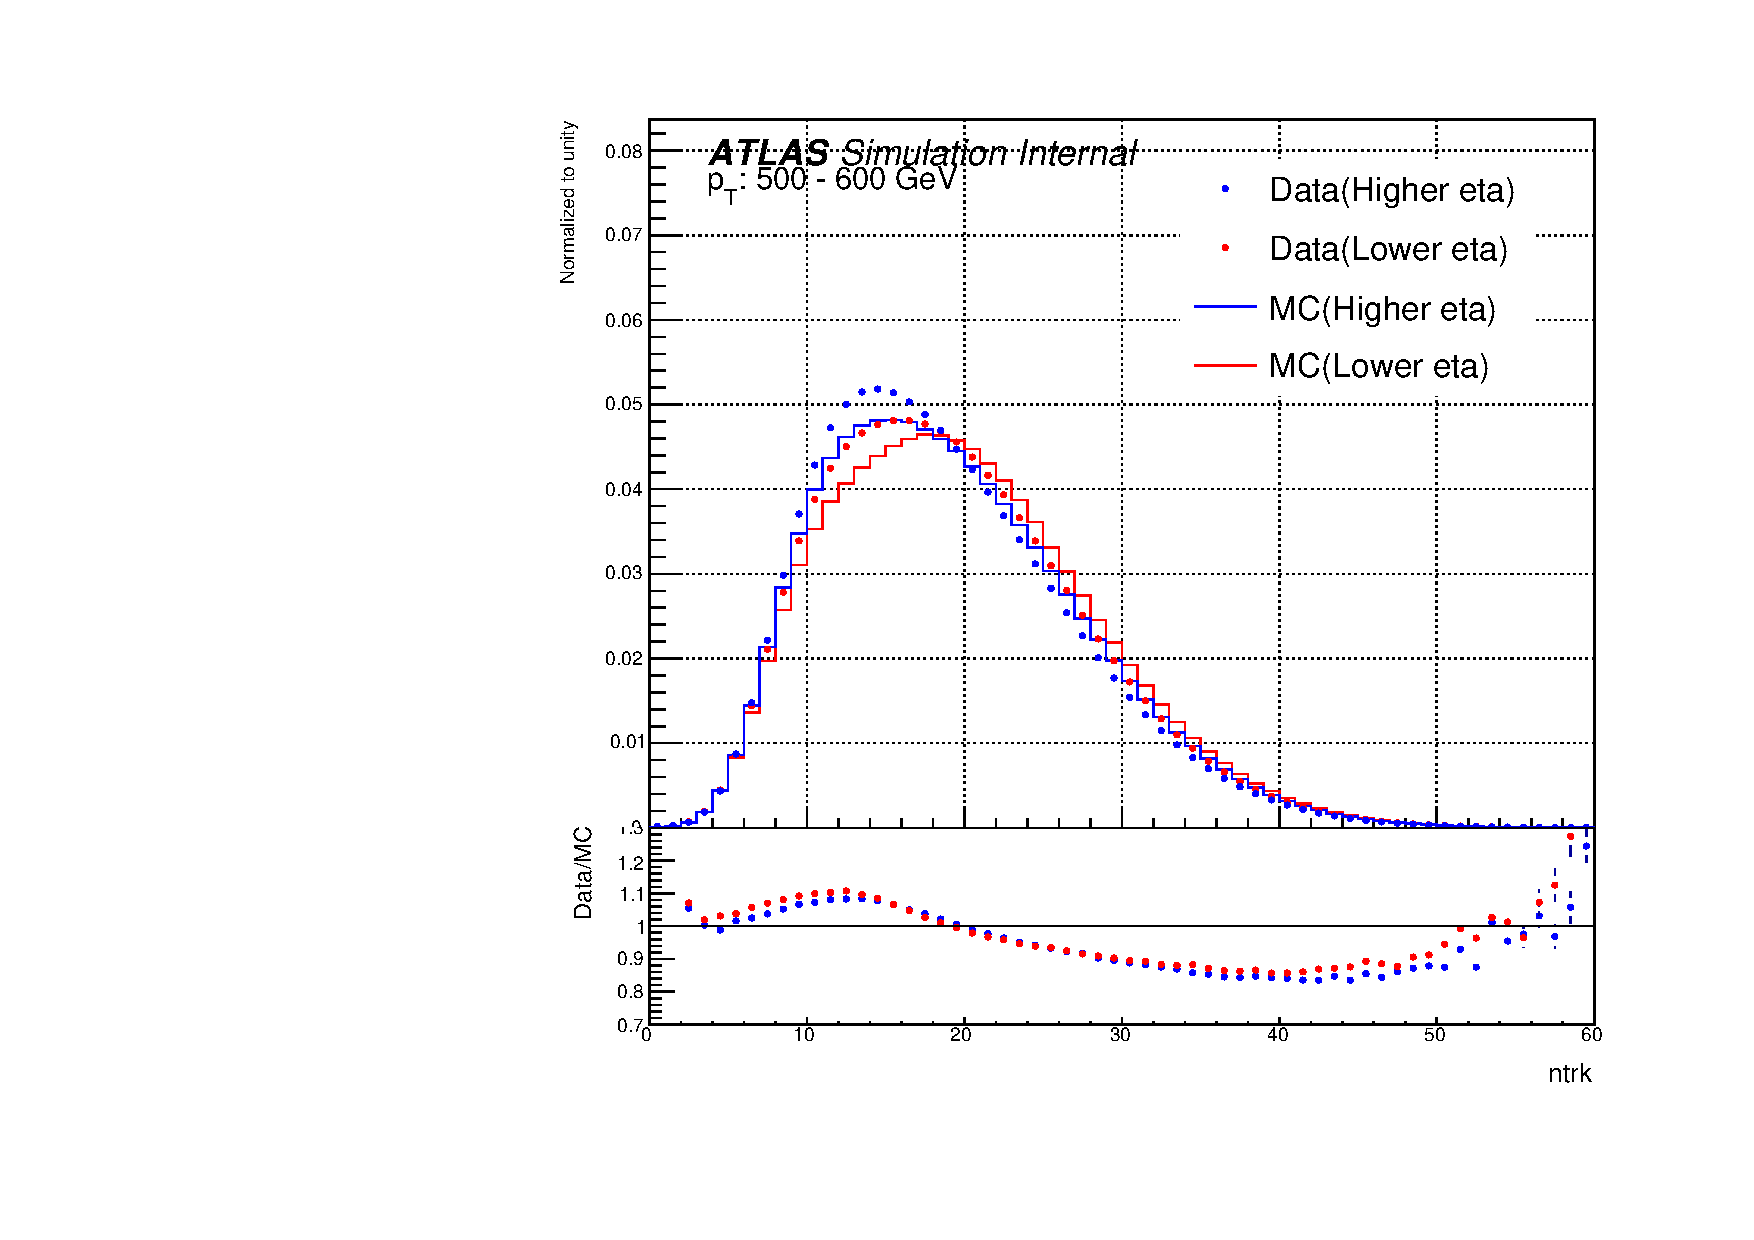
\includegraphics[width=0.45\textwidth]{Figures/dijetgammajetanalysis/MC_Closure/dist_comparison_plots/500-600_dist_total_comparison_ntrk_pythia}}
%	\caption[]{
%		The comparison between the data and MC with \sherpa  \subref{fig:QG-NtrkDataMCinclSherpaa} 	\subref{fig:QG-NtrkDataMCinclSherpab} and \pythia \subref{fig:QG-WtrkDataMCincla}  \subref{fig:QG-WtrkDataMCinclb} in \ntrk distributions of $\gamma$+jets and multi-jet events used in 2-sample extraction. %
%		Graphs and solid-line histograms show the \ntrk distributions in the data and MC, respectively.
%		Bottom panels show the ratio of the data to the MC in each of $\gamma$+jets and multi-jet events. %
%		\label{fig:QG-NtrkDataMCinclSherpa}
%	}
%\end{figure}
%
%\begin{figure}[htb]
%	\centering
%	\subfloat[$500<\pt<600\GeV$~(\sherpa) ]{\label{fig:QG-BDTDataMCinclSherpaa11}\includegraphics[width=0.45\textwidth]{Figures/dijetanalysis/higher-lower-sf/sherpa_MC_500_ntrk}} \quad
%	\subfloat[$800<\pt<1000\GeV$~(\sherpa)]{\label{fig:QG-BDTDataMCinclSherpab12}\includegraphics[width=0.45\textwidth]{Figures/dijetanalysis/higher-lower-sf/sherpa_MC_800_ntrk}}\\
%	\subfloat[$500<\pt<600\GeV$~(\pythia8) ]{\label{fig:QG-BDTDataMCinclPythiaa31}\includegraphics[width=0.45\textwidth]{Figures/dijetanalysis/higher-lower-sf/pythia_MC_500_ntrk}} \quad
%	\subfloat[$800<\pt<1000\GeV$~(\pythia8)]{\label{fig:QG-BDTDataMCinclPythiab41}\includegraphics[width=0.45\textwidth]{Figures/dijetanalysis/higher-lower-sf/pythia_MC_800_ntrk}}
%	\caption[]{
%		The comparison between the data and MC with \sherpa \subref{fig:QG-BDTDataMCinclSherpaa11} \subref{fig:QG-BDTDataMCinclSherpab21} and \pythia \subref{fig:QG-BDTDataMCinclPythiaa31} \subref{fig:QG-BDTDataMCinclPythiab41} in \nrtk distributions of higher or lower $\abseta$ multi-jet events used in 2-process extraction. %
%		Graphs and solid-line histograms show the \nrtk distributions in the data and MC, respectively.
%		Bottom panels show the ratio of the data to the MC in each of $\gamma$+jets and multi-jet events. %
%		\label{fig:QG-BDTDataMCinclPythia1}
%	}
%\end{figure}



%\begin{figure}[htb]
%	\centering
%	\subfloat[$50<\pt<600\GeV$~(\sherpa) ]{\label{fig:QG-WtrkDataMCinclaaa}\includegraphics[width=0.45\textwidth]{Figures/dijetanalysis/higher-lower-sf/sherpa_MC_500_ntrk}} \quad
%	\subfloat[$800<\pt<1000\GeV$~(\sherpa)]{\label{fig:QG-WtrkDataMCinclbbb}\includegraphics[width=0.45\textwidth]{Figures/dijetanalysis/higher-lower-sf/sherpa_MC_800_ntrk}}\\
%	\subfloat[$50<\pt<600\GeV$~(\pythia8) ]{\label{fig:QG-WtrkDataMCincla}\includegraphics[width=0.45\textwidth]{Figures/dijetanalysis/higher-lower-sf/pythia_MC_500_ntrk}} \quad
%	\subfloat[$800<\pt<1000\GeV$~(\pythia8)]{\label{fig:QG-WtrkDataMCinclb}\includegraphics[width=0.45\textwidth]{Figures/dijetanalysis/higher-lower-sf/pythia_MC_800_ntrk}}
%	\caption[]{
%		The comparison between the data and MC with \sherpa\subref{fig:QG-WtrkDataMCinclaaa} \subref{fig:QG-WtrkDataMCinclbbb} and \pythia \subref{fig:QG-WtrkDataMCincla} \subref{fig:QG-WtrkDataMCinclb} in \ntrk distributions of higher or lower $\abseta$ multi-jet events in 2-process extraction. %
%		Graphs and solid-line histograms show the \ntrk distributions in the data and MC, respectively.
%		Bottom panels show the ratio of the data to the MC in each of $\gamma$+jets and multi-jet events. %
%		\label{fig:QG-NtrkDataMCinclPythia}
%	}
%\end{figure}
%
%
%\begin{figure}[htb]
%	\centering
%	\subfloat[$100<\pt<150\GeV$~(\sherpa) ]{\label{fig:QG-WtrkDataMCinclSherpaa}\includegraphics[width=0.45\textwidth]{Figures/dijetgammajetanalysis/MC_Closure/dist_comparison_plots/100-150_dist_total_comparison_width_sherpa}} \quad
%	\subfloat[$500<\pt<600\GeV$~(\sherpa)]{\label{fig:QG-WtrkDataMCinclSherpab}\includegraphics[width=0.45\textwidth]{Figures/dijetgammajetanalysis/MC_Closure/dist_comparison_plots/500-600_dist_total_comparison_width_sherpa}}
%	\caption[]{
%		The comparison between the data and MC in \wtrk distributions of $\gamma$+jets and multi-jet events used in 2-sample extraction %
%		in \subref{fig:QG-WtrkDataMCinclSherpaa} the jet \pt range from 100 to 150\GeV and %
%		\subref{fig:QG-WtrkDataMCinclSherpab} from 500 to 600\GeV. %
%		Graphs and solid-line histograms show the \wtrk distributions in the data and MC, respectively.
%		Bottom panels show the ratio of the data to the MC in each of $\gamma$+jets and multi-jet events. %
%		\label{fig:QG-WtrkDataMCinclSherpa}
%	}
%\end{figure}
%
%\begin{figure}[htb]
%	\centering
%	\subfloat[$100<\pt<150\GeV$~(\pythia) ]{\label{fig:QG-WtrkDataMCinclSherpaa1}\includegraphics[width=0.45\textwidth]{Figures/dijetgammajetanalysis/MC_Closure/dist_comparison_plots/100-150_dist_total_comparison_width_pythia}} \quad
%	\subfloat[$500<\pt<600\GeV$~(\pythia)]{\label{fig:QG-WtrkDataMCinclSherpab1}\includegraphics[width=0.45\textwidth]{Figures/dijetgammajetanalysis/MC_Closure/dist_comparison_plots/500-600_dist_total_comparison_width_pythia}}
%	\caption[]{
%		The comparison between the data and MC in \wtrk distributions of $\gamma$+jets and multi-jet events used in 2-sample extraction %
%		in \subref{fig:QG-WtrkDataMCinclSherpaa} the jet \pt range from 100 to 150\GeV and %
%		\subref{fig:QG-WtrkDataMCinclSherpab} from 500 to 600\GeV. %
%		Graphs and solid-line histograms show the \wtrk distributions in the data and MC, respectively.
%		Bottom panels show the ratio of the data to the MC in each of $\gamma$+jets and multi-jet events. %
%		\label{fig:QG-WtrkDataMCinclSherpa1}
%	}
%\end{figure}
%
%\begin{figure}[htb]
%	\centering
%	\subfloat[$100<\pt<150\GeV$~(\sherpa) ]{\label{fig:QG-C1B02DataMCinclSherpaa}\includegraphics[width=0.45\textwidth]{Figures/dijetgammajetanalysis/MC_Closure/dist_comparison_plots/100-150_dist_total_comparison_c1_pythia}} \quad
%	\subfloat[$500<\pt<600\GeV$~(\sherpa)]{\label{fig:QG-C1B02DataMCinclSherpab}\includegraphics[width=0.45\textwidth]{Figures/dijetgammajetanalysis/MC_Closure/dist_comparison_plots/500-600_dist_total_comparison_c1_sherpa}}
%	\caption[]{
%		The comparison between the data and MC in \cbeta distributions of $\gamma$+jets and multi-jet events used in 2-sample extraction %
%		in \subref{fig:QG-C1B02DataMCinclSherpaa} the jet \pt range from 100 to 150\GeV and %
%		\subref{fig:QG-C1B02DataMCinclSherpab} from 500 to 600\GeV. %
%		Graphs and solid-line histograms show the \cbeta distributions in the data and MC, respectively.
%		Bottom panels show the ratio of the data to the MC in each of $\gamma$+jets and multi-jet events. %
%		\label{fig:QG-C1B02DataMCinclSherpa}
%	}
%\end{figure}
%
%\begin{figure}[htb]
%	\centering
%	\subfloat[$100<\pt<150\GeV$~(\pythia8) ]{\label{fig:QG-C1B02DataMCinclPythiaa}\includegraphics[width=0.45\textwidth]{Figures/dijetgammajetanalysis/MC_Closure/dist_comparison_plots/100-150_dist_total_comparison_c1_pythia}} \quad
%	\subfloat[$500<\pt<600\GeV$~(\pythia8)]{\label{fig:QG-C1B02DataMCinclPythiab}\includegraphics[width=0.45\textwidth]{Figures/dijetgammajetanalysis/MC_Closure/dist_comparison_plots/500-600_dist_total_comparison_c1_pythia}}
%	\caption[]{
%		The comparison between the data and MC in \cbeta distributions of $\gamma$ +jets and multi-jet events used in 2-sample extraction %
%		in \subref{fig:QG-C1B02DataMCinclPythiaa} the jet \pt range from 100 to 150\GeV and %
%		\subref{fig:QG-C1B02DataMCinclPythiab} from 500 to 600\GeV. %
%		Graphs and solid-line histograms show the \cbeta distributions in the data and MC, respectively.
%		Bottom panels show the ratio of the data to the MC in each of $\gamma$+jets and multi-jet events. %
%		\label{fig:QG-C1B02DataMCinclPythia}
%	}
%\end{figure}


%\begin{figure}[htb]
%	\centering
%	\subfloat[$100<\pt<150\GeV$~(\sherpa) ]{\label{fig:QG-BDTDataMCinclSherpaa}\includegraphics[width=0.45\textwidth]{Figures/dijetgammajetanalysis/MC_Closure/dist_comparison_plots/100-150_dist_total_comparison_bdt_sherpa}} \quad
%	\subfloat[$500<\pt<600\GeV$~(\sherpa)]{\label{fig:QG-BDTDataMCinclSherpab}\includegraphics[width=0.45\textwidth]{Figures/dijetgammajetanalysis/MC_Closure/dist_comparison_plots/500-600_dist_total_comparison_bdt_sherpa}}\\
%	\subfloat[$100<\pt<150\GeV$~(\pythia8) ]{\label{fig:QG-BDTDataMCinclPythiaa}\includegraphics[width=0.45\textwidth]{Figures/dijetgammajetanalysis/MC_Closure/dist_comparison_plots/100-150_dist_total_comparison_bdt_pythia}} \quad
%	\subfloat[$500<\pt<600\GeV$~(\pythia8)]{\label{fig:QG-BDTDataMCinclPythiab}\includegraphics[width=0.45\textwidth]{Figures/dijetgammajetanalysis/MC_Closure/dist_comparison_plots/500-600_dist_total_comparison_bdt_pythia}}
%	\caption[]{
%		The comparison between the data and MC with \sherpa \subref{fig:QG-BDTDataMCinclSherpaa} \subref{fig:QG-BDTDataMCinclSherpab} and \pythia \subref{fig:QG-BDTDataMCinclPythiaa} \subref{fig:QG-BDTDataMCinclPythiab}  in BDT distributions of $\gamma$+jets and multi-jet events used in 2-sample extraction.V. %
%		Graphs and solid-line histograms show the BDT distributions in the data and MC, respectively.
%		Bottom panels show the ratio of the data to the MC in each of $\gamma$+jets and multi-jet events. %
%		\label{fig:QG-BDTDataMCinclSherpa}
%	}
%\end{figure}
%\begin{figure}[htb]
%	\centering
%\subfloat[$500<\pt<600\GeV$~(\sherpa) ]{\label{fig:QG-BDTDataMCinclSherpaa1}\includegraphics[width=0.45\textwidth]{Figures/dijetanalysis/higher-lower-sf/sherpa_MC_500_bdt}} \quad
%\subfloat[$800<\pt<1000\GeV$~(\sherpa)]{\label{fig:QG-BDTDataMCinclSherpab2}\includegraphics[width=0.45\textwidth]{Figures/dijetanalysis/higher-lower-sf/sherpa_MC_800_bdt}}\\
%\subfloat[$500<\pt<600\GeV$~(\pythia8) ]{\label{fig:QG-BDTDataMCinclPythiaa3}\includegraphics[width=0.45\textwidth]{Figures/dijetanalysis/higher-lower-sf/pythia_MC_500_bdt}} \quad
%\subfloat[$800<\pt<1000\GeV$~(\pythia8)]{\label{fig:QG-BDTDataMCinclPythiab4}\includegraphics[width=0.45\textwidth]{Figures/dijetanalysis/higher-lower-sf/pythia_MC_800_bdt}}
%	\caption[]{
%		The comparison between the data and MC with \sherpa \subref{fig:QG-BDTDataMCinclSherpaa1} \subref{fig:QG-BDTDataMCinclSherpab2} and \pythia \subref{fig:QG-BDTDataMCinclPythiaa3} \subref{fig:QG-BDTDataMCinclPythiab4} in BDT distributions of higher or lower $\abseta$ multi-jet events used in 2-process extraction. %
%		Graphs and solid-line histograms show the BDT distributions in the data and MC, respectively.
%		Bottom panels show the ratio of the data to the MC in each of $\gamma$+jets and multi-jet events. %
%		\label{fig:QG-BDTDataMCinclPythia}
%	}
%\end{figure}

%\subsection{Method 2 for low \pt jet}
%\label{sec:method2_intro}
%\subsubsection{Prescale trigger}
%{\textcolor{red}{Wanyun and Rongqian: please add the study of prescale here for low pt dijet events}}
%The ATLAS trigger system consists of a hardware-based component, the Level-1 (L1), a software-based trigger system, the higher-level trigger (HLT) or Event Filter (EF). The HLT runs a simplified version of the ATLAS reconstruction software. On the HLT-level calibrated jets defined by the anti-kt algorithm with R = 0.4 are used. The calibration is close to the one of off-line jets. In this note the performance is evaluated with respect to PFlow jets.
%Each trigger item uses a L1 trigger and a HLT trigger. The L1 system first evaluates for each given trigger if it is passed. To keep the trigger rate at an acceptable level, the triggers with high trigger rate are only read-out for a fraction of all events ("prescales”). The prescale is a number applied on-line by the ATLAS trigger system. If an event passes the conditions set by the trigger system, the prescale for the L1 trigger and for the HLT trigger is decided. If the L1 or the HLT trigger is prescaled the HLT trigger decision is not evaluated in order to save computing time. The prescales for the L1 trigger and the HLT trigger are decided independently.
%The composition of the triggers used here is summarized in \Tab{tab:prescaletrigger}
%The jet \pT spectra for each of the triggers are shown in .{\textcolor{red}{Rongqian: please link jet triggers spectrum (before unprescaling) here}}\ref{fig:QG-b-ps}
%
%\begin{figure}[htb]
%	\centering
%	\subfloat[2017]{\label{fig:QG-2017ps}\includegraphics[width=0.45\textwidth]{Figures/Method2/Triggers/data17_single_trigger_Inclusive.pdf}}\quad
%	\subfloat[2018]{\label{fig:QG-2018ps}\includegraphics[width=0.45\textwidth]{Figures/Method2/Triggers/data18_single_trigger_Inclusive.pdf}}
%	\caption[]{
%	  The spectra for each jet trigger before unprescaling \subref{fig:QG-2017ps} is the 2017 dataset and \subref{fig:QG-b-ps} is the 2018 dataset.%
%		\label{fig:QG-b-ps}
%	}
%\end{figure}
%
%The jet \pT spectra can be corrected by the average prescale calculated by the ratio of luminosity collected by a given trigger and the total luminosity. The values in \href{https://aiatlas046.cern.ch/tagservices/RunBrowser/runBrowserReport/runBrowserReport.php?fnt=data18_13TeV&pn=*&cn=*}{COMA trigger report}are used. The corrected jet \pT spectra for each trigger are shown{\textcolor{red}{Rongqian: please link jet triggers spectrum (after unprescaling) here}}\ref{fig:QG-a-ps}
%
%\begin{figure}[htb]
%	\centering
%	\subfloat[2017]{\label{fig:QG-2017ps}\includegraphics[width=0.45\textwidth]{Figures/Method2/Triggers/data17single_trigger_InclusivePS.pdf}}\quad
%	\subfloat[2018]{\label{fig:QG-2018ps}\includegraphics[width=0.45\textwidth]{Figures/Method2/Triggers/data18single_trigger_InclusivePS.pdf}}
%	\caption[]{
%	  The spectra for each jet trigger after unprescaling \subref{fig:QG-2017ps} is the 2017 dataset and \subref{fig:QG-2018ps} is the 2018 dataset.%
%		\label{fig:QG-a-ps}
%	}
%\end{figure}
%
%\begin{table}[htb]
%	\centering
%	\caption{
%		The summary of the prescale HLT triggers used in this calibration. %
%	}
%	\begin{tabular}{c}
%		\whline
%		Trigger name \\
%		\hline
%		 HLT\_j35 \\
%		  HLT\_j45 \\
%		  HLT\_j60 \\
%		  HLT\_j110 \\
%		  HLT\_j175 \\
%		  HLT\_j260 \\
%		  HLT\_j360 \\
%		  \hline
%	 \end{tabular}
%	\label{tab:prescaletrigger}
%\end{table}
%
%
%
%{\textcolor{red}{Rongqian: please make the same plot in above section (method 1) for method 2 and put them here. Please put the plots in 100-150 and 400-500 GeV bins here and put others in appendix. }
%
%\begin{figure}[htb]
%	\centering
%	\subfloat[For $\gamma$+jets and multi-jet extraction~(\sherpa) ]{\label{fig:QG-Fmcc}\includegraphics[width=0.45\textwidth]{Figures/Method2/fraction/pt-fraction_pt.pdf}}\quad
%	\subfloat[For $\gamma$+jets and multi-jet extraction~(\pythia) ]{\label{fig:QG-Fmcd}\includegraphics[width=0.45\textwidth]{Figures/placeholder}}
%	\caption[]{
%	  (\textcolor{red}{Rongqian}) Fractions of quark jets and gluon jets in each of \subref{fig:QG-Fmcc} \subref{fig:QG-Fmcd} SHERPA and PYTHIA $\gamma$+jets and multi-jet for 2-process extraction %
%		$\gamma$+jets and multi-jets  %
%		These values are used as elements in $F$ matrix in \Eqn{eq:QG-matrix}(\ref{eq:QG-invmatrix}). %
%		\label{fig:QG-Fmc}
%	}
%\end{figure}
%
%
%\begin{figure}[htb]
%	\centering
%	\subfloat[$\gamma$+jets~(\sherpa)]{\label{fig:QG-jetMethod2Pta}\includegraphics[width=0.45\textwidth]{Figures/Method2/Pt-spectrum/GammaJet_Sherpa_pt_distribution.pdf}} \quad
%	\subfloat[multi-jet ~(\sherpa) ]{\label{fig:QG-jetHLPtb}\includegraphics[width=0.45\textwidth]{Figures/Method2/Pt-spectrum/LeadingJet_Dijet_Inclusive.png}}\\
%	\subfloat[$\gamma$+jets~(\pythia)]{\label{fig:QG-jetMethod2Ptaa}\includegraphics[width=0.45\textwidth]{Figures/placeholder}} \quad
%	\subfloat[multi-jet ~(\pythia) ]{\label{fig:QG-jetMethod2Ptbb}\includegraphics[width=0.45\textwidth]{Figures/placeholder}}
%%	\subfloat[$\gamma$+jets~(\sherpa)]{\label{fig:QG-jetMethod2Pta}\includegraphics[width=0.45\textwidth]{Figures/newplot/sherpa_higher_pt}} \quad
%%	\subfloat[multi-jet ~(\sherpa) ]{\label{fig:QG-jetMethod2Ptb}\includegraphics[width=0.45\textwidth]{Figures/newplot/sherpa_lower_pt}}\\
%%	\subfloat[$\gamma$+jets~(\pythia)]{\label{fig:QG-jetMethod2Ptaa}\includegraphics[width=0.45\textwidth]{Figures/dijetanalysis/pt-spectrum/powpyt_higher_pt}} \quad
%%	\subfloat[multi-jet ~(\pythia) ]{\label{fig:QG-jetMethod2Ptbb}\includegraphics[width=0.45\textwidth]{Figures/dijetanalysis/pt-spectrum/powpyt_lower_pt}}
%	\caption[]{
%	  (\textcolor{red}{Rongqian})The \pt distribution of the leading jets with \sherpa  \subref{fig:QG-jetMethod2Pta}  \subref{fig:QG-jetMethod2Ptb}  and \pythia 
%		 \subref{fig:QG-jetMethod2Ptaa}  \subref{fig:QG-jetMethod2Ptbb}  in  \subref{fig:QG-jetMethod2Pta} the $\gamma$+jets   %
%		and \subref{fig:QG-jetMethod2Ptb} the multi-jet extraction.
%	    %Data for four plots are 139\ifb in total.	The normalization of the simulation is decided by cross-section.
%		\label{fig:QG-jetMethod2Pt}
%	}
%\end{figure}
%
%\begin{figure}[htb]
%	\centering
%	\subfloat[$\gamma$+jets~(\sherpa)]{\label{fig:QG-jetHLPta}\includegraphics[width=0.45\textwidth]{Figures/Method2/kinematics/Gammajet-eta.png}} \quad
%	\subfloat[multi-jet~(\sherpa) ]{\label{fig:QG-jetHLPtb}\includegraphics[width=0.45\textwidth]{Figures/Method2/kinematics/Dijet_Sherpa_eta.png}}\\
%	\subfloat[$\gamma$+jets~(\pythia)]{\label{fig:QG-jetHLPtaa}\includegraphics[width=0.45\textwidth]{Figures/placeholder}} \quad
%	\subfloat[multi-jet~(\pythia) ]{\label{fig:QG-jetHLPtbb}\includegraphics[width=0.45\textwidth]{Figures/placeholder}}
%%	\subfloat[$\gamma$+jets~(\sherpa)]{\label{fig:QG-jetHLPta}\includegraphics[width=0.45\textwidth]{Figures/newplot/sherpa_higher_pt}} \quad
%%	\subfloat[Lower \abseta jet~(\sherpa) ]{\label{fig:QG-jetHLPtb}\includegraphics[width=0.45\textwidth]{Figures/newplot/sherpa_lower_pt}}\\
%%	\subfloat[Higher \abseta jet~(\pythia)]{\label{fig:QG-jetHLPtaa}\includegraphics[width=0.45\textwidth]{Figures/dijetanalysis/pt-spectrum/powpyt_higher_pt}} \quad
%%	\subfloat[Lower \abseta jet~(\pythia) ]{\label{fig:QG-jetHLPtbb}\includegraphics[width=0.45\textwidth]{Figures/dijetanalysis/pt-spectrum/powpyt_lower_pt}}
%	\caption[]{
%	  (\textcolor{red}{Rongqian})The \eta distribution of the jets with \sherpa  \subref{fig:QG-jetHLPta}  \subref{fig:QG-jetHLPtb}  and \pythia 
%		 \subref{fig:QG-jetHLPtaa}  \subref{fig:QG-jetHLPtbb}  in  \subref{fig:QG-jetHLPta} the $\gamma$+jets   %
%		and \subref{fig:QG-jetHLPtb} the multi-jet extraction.
%	    %Data for four plots are 139\ifb in total.	The normalization of the simulation is decided by cross-section.
%		\label{fig:QG-eta-method1}
%	}
%\end{figure}
%
%\begin{figure}[htb]
%	\centering
%	\subfloat[$\gamma$+jets~(\sherpa)]{\label{fig:QG-jetHLPta}\includegraphics[width=0.45\textwidth]{Figures/Method2/kinematics/Gammajet-ntrk.png}} \quad
%	\subfloat[multi-jet~(\sherpa) ]{\label{fig:QG-jetHLPtb}\includegraphics[width=0.45\textwidth]{Figures/Method2/kinematics/Dijet_Sherpa_ntrk.png}}\\
%	\subfloat[$\gamma$+jets~(\pythia)]{\label{fig:QG-jetHLPtaa}\includegraphics[width=0.45\textwidth]{Figures/placeholder}} \quad
%	\subfloat[multi-jet~(\pythia) ]{\label{fig:QG-jetHLPtbb}\includegraphics[width=0.45\textwidth]{Figures/placeholder}}
%%	\subfloat[Higher \abseta jet~(\sherpa)]{\label{fig:QG-jetHLPta}\includegraphics[width=0.45\textwidth]{Figures/newplot/sherpa_higher_pt}} \quad
%%	\subfloat[Lower \abseta jet~(\sherpa) ]{\label{fig:QG-jetHLPtb}\includegraphics[width=0.45\textwidth]{Figures/newplot/sherpa_lower_pt}}\\
%%	\subfloat[Higher \abseta jet~(\pythia)]{\label{fig:QG-jetHLPtaa}\includegraphics[width=0.45\textwidth]{Figures/dijetanalysis/pt-spectrum/powpyt_higher_pt}} \quad
%%	\subfloat[Lower \abseta jet~(\pythia) ]{\label{fig:QG-jetHLPtbb}\includegraphics[width=0.45\textwidth]{Figures/dijetanalysis/pt-spectrum/powpyt_lower_pt}}
%	\caption[]{
%	  (\textcolor{red}{Rongqian})The \ntrk distribution of the jets with \sherpa  \subref{fig:QG-jetHLPta}  \subref{fig:QG-jetHLPtb}  and \pythia 
%		 \subref{fig:QG-jetHLPtaa}  \subref{fig:QG-jetHLPtbb}  in  \subref{fig:QG-jetHLPta} the $\gamma$+jets   %
%		and \subref{fig:QG-jetHLPtb} the multi-jet extraction.
%	    %Data for four plots are 139\ifb in total.	The normalization of the simulation is decided by cross-section.
%		\label{fig:QG-ntrk-method1}
%	}
%\end{figure}
%
%\begin{figure}[htb]
%	\centering
%	\subfloat[$\gamma$+jets~(\sherpa)]{\label{fig:QG-jetHLPta}\includegraphics[width=0.45\textwidth]{Figures/Method2/kinematics/Gammajet-width.png}} \quad
%	\subfloat[multi-jet~(\sherpa) ]{\label{fig:QG-jetHLPtb}\includegraphics[width=0.45\textwidth]{Figures/Method2/kinematics/Dijet_Sherpa_width.png}}\\
%	\subfloat[$\gamma$+jets~(\pythia)]{\label{fig:QG-jetHLPtaa}\includegraphics[width=0.45\textwidth]{Figures/placeholder}} \quad
%	\subfloat[multi-jet~(\pythia) ]{\label{fig:QG-jetHLPtbb}\includegraphics[width=0.45\textwidth]{Figures/placeholder}}
%%	\subfloat[Higher \abseta jet~(\sherpa)]{\label{fig:QG-jetHLPta}\includegraphics[width=0.45\textwidth]{Figures/newplot/sherpa_higher_pt}} \quad
%%	\subfloat[Lower \abseta jet~(\sherpa) ]{\label{fig:QG-jetHLPtb}\includegraphics[width=0.45\textwidth]{Figures/newplot/sherpa_lower_pt}}\\
%%	\subfloat[Higher \abseta jet~(\pythia)]{\label{fig:QG-jetHLPtaa}\includegraphics[width=0.45\textwidth]{Figures/dijetanalysis/pt-spectrum/powpyt_higher_pt}} \quad
%%	\subfloat[Lower \abseta jet~(\pythia) ]{\label{fig:QG-jetHLPtbb}\includegraphics[width=0.45\textwidth]{Figures/dijetanalysis/pt-spectrum/powpyt_lower_pt}}
%	\caption[]{
%	  (\textcolor{red}{Rongqian})The \wtrk distribution of the leading jets with \sherpa  \subref{fig:QG-jetHLPta}  \subref{fig:QG-jetHLPtb}  and \pythia 
%		 \subref{fig:QG-jetHLPtaa}  \subref{fig:QG-jetHLPtbb}  in  \subref{fig:QG-jetHLPta} the $\gamma$+jets   %
%		and \subref{fig:QG-jetHLPtb} the multi-jet extraction.
%	    %Data for four plots are 139\ifb in total.	The normalization of the simulation is decided by cross-section.
%		\label{fig:QG-wtrk-methed1}
%	}
%\end{figure}
%
%\begin{figure}[htb]
%	\centering
%	\subfloat[$\gamma$+jets~(\sherpa)]{\label{fig:QG-jetHLPta}\includegraphics[width=0.45\textwidth]{Figures/Method2/kinematics/Gammajet-c1.png}} \quad
%	\subfloat[multi-jet~(\sherpa) ]{\label{fig:QG-jetHLPtb}\includegraphics[width=0.45\textwidth]{Figures/Method2/kinematics/Dijet_Sherpa_c1.png}}\\
%	\subfloat[$\gamma$+jets~(\pythia)]{\label{fig:QG-jetHLPtaa}\includegraphics[width=0.45\textwidth]{Figures/placeholder}} \quad
%	\subfloat[multi-jet jet~(\pythia) ]{\label{fig:QG-jetHLPtbb}\includegraphics[width=0.45\textwidth]{Figures/placeholder}}
%%	\subfloat[Higher \abseta jet~(\sherpa)]{\label{fig:QG-jetHLPta}\includegraphics[width=0.45\textwidth]{Figures/newplot/sherpa_higher_pt}} \quad
%%	\subfloat[Lower \abseta jet~(\sherpa) ]{\label{fig:QG-jetHLPtb}\includegraphics[width=0.45\textwidth]{Figures/newplot/sherpa_lower_pt}}\\
%%	\subfloat[Higher \abseta jet~(\pythia)]{\label{fig:QG-jetHLPtaa}\includegraphics[width=0.45\textwidth]{Figures/dijetanalysis/pt-spectrum/powpyt_higher_pt}} \quad
%%	\subfloat[Lower \abseta jet~(\pythia) ]{\label{fig:QG-jetHLPtbb}\includegraphics[width=0.45\textwidth]{Figures/dijetanalysis/pt-spectrum/powpyt_lower_pt}}
%	\caption[]{
%	  (\textcolor{red}{Rongqian})The C1 distribution of the jets with \sherpa  \subref{fig:QG-jetHLPta}  \subref{fig:QG-jetHLPtb}  and \pythia 
%		 \subref{fig:QG-jetHLPtaa}  \subref{fig:QG-jetHLPtbb}  in  \subref{fig:QG-jetHLPta} the $\gamma$+jets   %
%		and \subref{fig:QG-jetHLPtb} the multi-jet extraction.
%	    %Data for four plots are 139\ifb in total.	The normalization of the simulation is decided by cross-section.
%		\label{fig:QG-wtrk-methed1}
%	}
%\end{figure}
%
%\begin{figure}[htb]
%	\centering
%	\subfloat[$100<\pt<150\GeV$~(\sherpa) ]{\label{fig:QG-NtrkDataMCinclSherpaa}\includegraphics[width=0.45\textwidth]{Figures/Method2/SF-MC/100-150_dist_total_comparison_ntrk_sherpa.pdf}} \quad
%	\subfloat[400<\pt<500\GeV$~(\sherpa)]{\label{fig:QG-NtrkDataMCinclSherpab}\includegraphics[width=0.45\textwidth]{Figures/Method2/SF-MC/400-500_dist_total_comparison_ntrk_sherpa.pdf}}\\
%	\subfloat[$100<\pt<150\GeV$~(\pythia8) ]{\label{fig:QG-WtrkDataMCincla}\includegraphics[width=0.45\textwidth]{Figures/Method2/SF-MC/}} \quad
%	\subfloat[$400<\pt<500\GeV$~(\pythia8)]{\label{fig:QG-WtrkDataMCinclb}\includegraphics[width=0.45\textwidth]{Figures/Method2/SF-MC/}}
%	\caption[]{
%		The comparison between the data and MC with \sherpa  \subref{fig:QG-NtrkDataMCinclSherpaa} 	\subref{fig:QG-NtrkDataMCinclSherpab} and \pythia \subref{fig:QG-WtrkDataMCincla}  \subref{fig:QG-WtrkDataMCinclb} in \ntrk distributions of $\gamma$+jets and multi-jet events used in 2-sample extraction. %
%		Graphs and solid-line histograms show the \ntrk distributions in the data and MC, respectively.
%		Bottom panels show the ratio of the data to the MC in each of $\gamma$+jets and multi-jet events. %
%		\label{fig:QG-NtrkDataMCinclSherpa}
%	}
%\end{figure}
%
%\begin{figure}[htb]
%	\centering
%	\subfloat[$100<\pt<150\GeV$~(\sherpa) ]{\label{fig:QG-NtrkDataMCinclSherpaa}\includegraphics[width=0.45\textwidth]{Figures/Method2/SF-MC/100-150_dist_total_comparison_bdt_sherpa.pdf}} \quad
%	\subfloat[400<\pt<500\GeV$~(\sherpa)]{\label{fig:QG-NtrkDataMCinclSherpab}\includegraphics[width=0.45\textwidth]{Figures/Method2/SF-MC/400-500_dist_total_comparison_bdt_sherpa.pdf}}\\
%	\subfloat[$100<\pt<150\GeV$~(\pythia8) ]{\label{fig:QG-WtrkDataMCincla}\includegraphics[width=0.45\textwidth]{Figures/Method2/SF-MC/}} \quad
%	\subfloat[$400<\pt<500\GeV$~(\pythia8)]{\label{fig:QG-WtrkDataMCinclb}\includegraphics[width=0.45\textwidth]{Figures/Method2/SF-MC/}}
%	\caption[]{
%		The comparison between the data and MC with \sherpa  \subref{fig:QG-NtrkDataMCinclSherpaa} 	\subref{fig:QG-NtrkDataMCinclSherpab} and \pythia \subref{fig:QG-WtrkDataMCincla}  \subref{fig:QG-WtrkDataMCinclb} in BDT distributions of $\gamma$+jets and multi-jet events used in 2-sample extraction. %
%		Graphs and solid-line histograms show the BDT distributions in the data and MC, respectively.
%		Bottom panels show the ratio of the data to the MC in each of $\gamma$+jets and multi-jet events. %
%		\label{fig:QG-NtrkDataMCinclSherpa}
%	}
%\end{figure}
%
%\begin{figure}[htb]
%	\centering
%	\subfloat[$100<\pt<150\GeV$~(\sherpa) ]{\label{fig:QG-BDT1}\includegraphics[width=0.45\textwidth]{Figures/Method2/roc/plots/roc-var/ROC_100-150_dijet.pdf}} \quad
%	\subfloat[400<\pt<500\GeV$~(\sherpa)]{\label{fig:QG-BDT2}\includegraphics[width=0.45\textwidth]{Figures/Method2/roc/plots/roc-var/ROC_400-500_dijet.pdf}}\\
%	\subfloat[$100<\pt<150\GeV$~(\pythia8) ]{\label{fig:QG-WtrkDataMCincla}\includegraphics[width=0.45\textwidth]{Figures/Method2/SF-MC/}} \quad
%	\subfloat[$400<\pt<500\GeV$~(\pythia8)]{\label{fig:QG-WtrkDataMCinclb}\includegraphics[width=0.45\textwidth]{Figures/Method2/SF-MC/}}
%	\caption[]{
%		ROC curve for different jet taggers%
%		\label{fig:QG-NtrkDataMCinclSherpa}
%	}
%\end{figure}
%
%
%\subsubsection{Background study}
%{\textcolor{red}{Wanyun and Rongqian: please add the background study here (ABCD) and tell people the background for dijet is negiligible}}
%
%
%
%\subsection{Validation} (\textcolor{red}{let's skip this section for now})
%\label{subsec:Validation }
%
%In addition to the primary samples defined above, several samples with very high quark or gluon-jet fractions are defined to validate the extracted templates in different topologies. The high purity is achieved by the use of event-level kinematic cuts. One is trijet sample used for validation of the extracted gluon template, Events are required to have a leading jet which passes the lowest unprescaled single jet trigger and a pT of at least 500 GeV. There must be at least two additional jets with \pT $>$ 20 GeV. All three jets must have $\abseta$ $<$ 2.1. The third jet is very likely to be gluon initiated in certain regions of phase space. The other one is $\gamma$+2jets sample, which has high quark-jet purity,The basic event selection is the same as for the $\gamma$+jet sample, with the exceptions that there should be at least one sub-leading jet with \pT > 20 GeV and $\abseta$ $<$ 2.1. 
\FloatBarrier


\subsection{MC non-closure}
\label{sec:QG-closure}
 
  The matrix method is valid under the assumption that the shapes of $p_{\mrm{Q}}(x)$ and $p_{\mrm{G}}(x)$ emain consistent, regardless of whether the jets are situated in the central or forward regions. Jet fragmentation at a $pp$ collider is expected to be predominantly influenced by the jet \pt~and is generally considered independent of $\eta$, considering the underlying parton type. Consequently, an approach aimed at extracting distributions associated with the radiation patterns of quark-jets and gluon-jets should be valid at the particle level. At the detector level, however, the measured radiation pattern within jets no longer retains its $\eta$-independence. This is due to variations arising from differences in detector materials and technologies, leading to distinctions between the central and forward regions in terms of response. As a consequence of these effects, the matrix method experiences deviations from closure,, indicating a disparity between the expected and actual outcomes.
  


The distributions of {\ntrk} have been seen to have systematic difference for the truth-labelled quark/gluon jets in the quark-enriched and gluon-enriched regions in each \pt~bin. To rectify this discrepancy and ensure alignment in the distribution of jet tagging variables between the central and forward regions, a re-weighting procedure is implemented. This procedure involves applying adjustments to account for the observed differences.  For each event, the central jet is weighted by a re-weighting factor :
\begin{equation}
%w_{\mrm{Q/G}}({x;p_{\text{T,j}}}) = \frac{ p_{\mrm{Q/G,~higher \abseta}}({x;p_{\text{T,j}}}) }{ p_{\mrm{Q/G,~lower \abseta}}({x;p_{\text{T,j}}})}
w_{\mathrm{Q} / \mathrm{G}}\left(x ; p_{\mathrm{T}, \mathrm{j}}\right)=\frac{p_{\mathrm{Q} / \mathrm{G}, \text { forward }}\left(x ; p_{\mathrm{T}, \mathrm{j}}\right)}{p_{\mathrm{Q} / \mathrm{G}, \text { central }}\left(x ; p_{\mathrm{T}, \mathrm{j}}\right)}
\label{eq:QG-reweight}
\end{equation}
where $q/g$ tagging variable $x$ is calculated in each jet \pt~bin for quark and gluon jets, respectively. By default the re-weighting factor derived from truth-labelled quark-jets is implemented for both types of jets, whereas the re-weighting factor derived from truth-labelled gluon-jets is used as an alternative to evaluate the systematic uncertainty from the re-weighting procedure, known as MC non-closure systematic uncertainty for the calibration.



The distributions of \ntrk~in extracted pure quark- and gluon-jets and truth-labelled MC before re-weighting as shown in Figure~\ref{fig:QG-pythia-NtrkMCExtractedNoReweight-Ntrk}. After the re-weighting the distributions of \ntrk~are shown in Figure~\ref{fig:QG-pythia-NtrkMCExtractedQuarkFactor-Ntrk}. The non-closure is at few percent level and is is taken as MC non-closure systematic uncertainty. 

\begin{figure}[htb]
	\centering
	\subfloat[ ]{\label{fig:QG-pythia-QuarkNtrkMCExtractedNoReweight-500-600-Ntrk}\includegraphics[width=0.45\textwidth]{fig/ADE/MCClosure/none_event_weight/jet_nTracks/MCClosure_500_quark_jet_nTracks.pdf}} \quad
	\subfloat[ ]{\label{fig:QG-pythia-GluonNtrkMCExtractedNoReweight-500-600-Ntrk}\includegraphics[width=0.45\textwidth]{fig/ADE/MCClosure/none_event_weight/jet_nTracks/MCClosure_500_gluon_jet_nTracks.pdf}} \\
	\subfloat[ ]{\label{fig:QG-pythia-QuarkNtrkMCExtractedNoReweight-800-1000-Ntrk}\includegraphics[width=0.45\textwidth]{fig/ADE/MCClosure/none_event_weight/jet_nTracks/MCClosure_800_quark_jet_nTracks.pdf}} \quad
	\subfloat[ ]{\label{fig:QG-pythia-GluonNtrkMCExtractedNoReweight-800-1000-Ntrk}\includegraphics[width=0.45\textwidth]{fig/ADE/MCClosure/none_event_weight/jet_nTracks/MCClosure_800_gluon_jet_nTracks.pdf}} \\
	\caption[]{
		Before re-weighting: the {\ntrk} distributions of quark-jet \subref{fig:QG-pythia-QuarkNtrkMCExtractedNoReweight-500-600-Ntrk}  \subref{fig:QG-pythia-QuarkNtrkMCExtractedNoReweight-800-1000-Ntrk} 
		and  gluon-jet in \subref{fig:QG-pythia-GluonNtrkMCExtractedNoReweight-500-600-Ntrk}  \subref{fig:QG-pythia-GluonNtrkMCExtractedNoReweight-800-1000-Ntrk} 
		 from {\pythia8} sample. %
		Dashed and solid-line show the {\ntrk} distributions in the truth MC and extracted MC, respectively.
		Bottom panels show the ratio of the extracted MC to the truth MC. %
		\label{fig:QG-pythia-NtrkMCExtractedNoReweight-Ntrk}
	}
\end{figure}



\begin{figure}[htb]
	\centering
	\subfloat[ ]{\label{fig:QG-pythia-QuarkNtrkMCExtractedQuarkFactor-Ntrk-500-600-Ntrk}\includegraphics[width=0.45\textwidth]{fig/ADE/MCClosure/jet_nTracks_quark_reweighting_weights/jet_nTracks/MCClosure_500_quark_jet_nTracks.pdf}} \quad
	\subfloat[ ]{\label{fig:QG-pythia-GluonNtrkMCExtractedQuarkFactor-Ntrk-500-600-Ntrk}\includegraphics[width=0.45\textwidth]{fig/ADE/MCClosure/jet_nTracks_quark_reweighting_weights/jet_nTracks/MCClosure_500_gluon_jet_nTracks.pdf}} \\
	\subfloat[ ]{\label{fig:QG-pythia-QuarkNtrkMCExtractedEQuarkFactor-Ntrk-800-1000-Ntrk}\includegraphics[width=0.45\textwidth]{fig/ADE/MCClosure/jet_nTracks_quark_reweighting_weights/jet_nTracks/MCClosure_800_quark_jet_nTracks.pdf}} \quad
	\subfloat[ ]{\label{fig:QG-pythia-GluonNtrkMCExtractedQuDarkFactor-Ntrk-800-1000-Ntrk}\includegraphics[width=0.45\textwidth]{fig/ADE/MCClosure/jet_nTracks_quark_reweighting_weights/jet_nTracks/MCClosure_800_gluon_jet_nTracks.pdf}} \\
	\caption[]{
		After re-weighting with quark factor: the {\ntrk} distributions of quark-jet \subref{fig:QG-pythia-QuarkNtrkMCExtractedQuarkFactor-Ntrk-500-600-Ntrk} \subref{fig:QG-pythia-QuarkNtrkMCExtractedEQuarkFactor-Ntrk-800-1000-Ntrk} 
		and gluon-jet in \subref{fig:QG-pythia-GluonNtrkMCExtractedQuarkFactor-Ntrk-500-600-Ntrk} \subref{fig:QG-pythia-GluonNtrkMCExtractedQuDarkFactor-Ntrk-800-1000-Ntrk}
		 from {\pythia8} sample. %
		Dashed and solid-line show the {\ntrk} distributions in the truth MC and extracted MC, respectively.
		Bottom panels show the ratio of the extracted MC to the truth MC. %
		\label{fig:QG-pythia-NtrkMCExtractedQuarkFactor-Ntrk}
	}
\end{figure}

\FloatBarrier

\subsubsection{Closure test for BDT tagger}
Similar to the distribution of {\ntrk}, the distributions of BDT score for truth labelled-jets exhibit systematic disparities in forward and central regions. Therefore, the same re-weighting procedure as described is performed for BDT tagger as well. The MC non-closure test is thus conducted by comparing the distributions of BDT score for extracted and truth quark- and gluon-jets, separately, as shown in Figure~\ref{fig:QG-pythia-BDTMCExtracted-Reweight-Compare1}. The distributions of BDT before and after re-weighting are shown in Figure~\ref{fig:QG-pythia-BDTMCExtractedNoReweight} and Figure~\ref{fig:QG-pythia-BDTMCExtractedQuarkFactor-BDT}. The non-closure is about few percent level and taken as one systematic uncertainty.

\begin{figure}[htb]
	\centering
	\subfloat[ ]{\label{fig:QG-pythia-BDTMCExtractedNoreweight-500-600-BDT}\includegraphics[width=0.45\textwidth]{fig/ADE/FvsC/none_event_weight/GBDT_newScore/MC_truth_Q_G_FvsC_500_GBDT_newScore_event_weight.pdf}} \quad
	\subfloat[ ]{\label{fig:QG-pythia-BDTMCExtractedQuarkFactor-500-600-BDT}\includegraphics[width=0.45\textwidth]{fig/ADE/FvsC/GBDT_newScore_quark_reweighting_weights/GBDT_newScore/MC_truth_Q_G_FvsC_500_GBDT_newScore_quark_reweighting_weights.pdf}} \\
	\subfloat[ ]{\label{fig:QG-pythia-BDTMCExtractedNoreweight-800-1000-BDT}\includegraphics[width=0.45\textwidth]{fig/ADE/FvsC/none_event_weight/GBDT_newScore/MC_truth_Q_G_FvsC_800_GBDT_newScore_event_weight.pdf}} \quad
	\subfloat[ ]{\label{fig:QG-pythia-BDTMCExtractedQuarkFactor-800-1000-BDT}\includegraphics[width=0.45\textwidth]{fig/ADE/FvsC/GBDT_newScore_quark_reweighting_weights/GBDT_newScore/MC_truth_Q_G_FvsC_800_GBDT_newScore_quark_reweighting_weights.pdf}} \\
	\caption[]{
		The distribution of BDT score for jets
		before \subref{fig:QG-pythia-BDTMCExtractedNoreweight-500-600-BDT} \subref{fig:QG-pythia-BDTMCExtractedNoreweight-800-1000-BDT} and 
		after \subref{fig:QG-pythia-BDTMCExtractedQuarkFactor-500-600-BDT} \subref{fig:QG-pythia-BDTMCExtractedQuarkFactor-800-1000-BDT} re-weighting. 
		\label{fig:QG-pythia-BDTMCExtracted-Reweight-Compare1}
	}
	
\end{figure}



%
\begin{figure}[htb]
	\centering
	\subfloat[ ]{\label{fig:QG-pythia-QuarkBDTMCExtractedNoReweight-500-600-BDT}\includegraphics[width=0.45\textwidth]{fig/ADE/MCClosure/none_event_weight/GBDT_newScore/MCClosure_500_quark_GBDT_newScore.pdf}} \quad
	\subfloat[ ]{\label{fig:QG-pythia-GluonBDTMCExtractedNoReweight-500-600-BDT}\includegraphics[width=0.45\textwidth]{fig/ADE/MCClosure/none_event_weight/GBDT_newScore/MCClosure_500_gluon_GBDT_newScore.pdf}} \\
	\subfloat[ ]{\label{fig:QG-pythia-QuarkBDTMCExtractedNoReweight-800-1000-BDT}\includegraphics[width=0.45\textwidth]{fig/ADE/MCClosure/none_event_weight/GBDT_newScore/MCClosure_800_quark_GBDT_newScore.pdf}} \quad
	\subfloat[ ]{\label{fig:QG-pythia-GluonBDTMCExtractedNoReweight-800-1000-BDT}\includegraphics[width=0.45\textwidth]{fig/ADE/MCClosure/none_event_weight/GBDT_newScore/MCClosure_800_gluon_GBDT_newScore.pdf}} \\
	\caption[]{
		Before re-weighting: the MC-closure for quark-jet in \subref{fig:QG-pythia-QuarkBDTMCExtractedNoReweight-500-600-BDT} \subref{fig:QG-pythia-QuarkBDTMCExtractedNoReweight-800-1000-BDT}  
		and for gluon-jet in \subref{fig:QG-pythia-GluonBDTMCExtractedNoReweight-500-600-BDT}  \subref{fig:QG-pythia-GluonBDTMCExtractedNoReweight-800-1000-BDT} 
		in BDT distributions from {\pythia8} sample. %
		Dashed and solid-line histograms show the BDT distributions in the truth MC and extracted MC, respectively.
		Bottom panels show the ratio of the extracted MC to the truth MC. %
		\label{fig:QG-pythia-BDTMCExtractedNoReweight}
	}
\end{figure}



\begin{figure}[htb]
	\centering
	\subfloat[ ]{\label{fig:QG-pythia-QuarkBDTMCExtractedQuarkFactor-BDT-500-600-BDT}\includegraphics[width=0.45\textwidth]{fig/ADE/MCClosure/GBDT_newScore_quark_reweighting_weights/GBDT_newScore/MCClosure_500_quark_GBDT_newScore.pdf}} \quad
	\subfloat[ ]{\label{fig:QG-pythia-GluonBDTMCExtractedQuarkFactor-BDT-500-600-BDT}\includegraphics[width=0.45\textwidth]{fig/ADE/MCClosure/GBDT_newScore_quark_reweighting_weights/GBDT_newScore/MCClosure_500_gluon_GBDT_newScore.pdf}} \\
	\subfloat[ ]{\label{fig:QG-pythia-QuarkBDTMCExtractedQuarkFactor-BDT-800-1000-BDT}\includegraphics[width=0.45\textwidth]{fig/ADE/MCClosure/GBDT_newScore_quark_reweighting_weights/GBDT_newScore/MCClosure_800_quark_GBDT_newScore.pdf}} \quad
	\subfloat[ ]{\label{fig:QG-pythia-GluonBDTMCExtractedQuarkFactor-BDT-800-1000-BDT}\includegraphics[width=0.45\textwidth]{fig/ADE/MCClosure/GBDT_newScore_quark_reweighting_weights/GBDT_newScore/MCClosure_800_gluon_GBDT_newScore.pdf}} \\
	\caption[]{
		After re-weighting: the MC-closure for quark-jet in \subref{fig:QG-pythia-QuarkBDTMCExtractedQuarkFactor-BDT-500-600-BDT} \subref{fig:QG-pythia-QuarkBDTMCExtractedQuarkFactor-BDT-800-1000-BDT} 
		and for gluon-jet in \subref{fig:QG-pythia-GluonBDTMCExtractedQuarkFactor-BDT-500-600-BDT}  \subref{fig:QG-pythia-GluonBDTMCExtractedQuarkFactor-BDT-800-1000-BDT} in BDT distributions from {\pythia8} sample. %
		Dashed and solid-line histograms show the BDT distributions in the truth MC and extracted MC, respectively.
		Bottom panels show the ratio of the extracted MC to the truth MC. %
		\label{fig:QG-pythia-BDTMCExtractedQuarkFactor-BDT}
	}
\end{figure}





\FloatBarrier

\subsubsection{Summary for the MC Closure test}
\label{sec:mcclosure-summary}
After applied the re-weighting factor to the jet tagging variables {\ntrk} and BDT, the distributions of extracted quark-and gluon-jets converge with those of truth jets. The residual discrepancy, which has only few percent level to the total events is taken into account as MC non-closure systematic uncertainty. No obvious dependency on jet $\eta$ is observed from the distributions of jet tagging variables.



\subsection{Scale factor}
\label{sec:QG-SF}
The calibration of the q/g tagging variables is performed by applying binned scale factor (SF) in the simulation for each quark- and gluon-jet, respectively. The scale factor is obtained from distributions of the variables in quark- and gluon-jets from MC in order to match the shape of the simulation to that of the data. 

The tagger working points (WP) are established for fixed quark-jets efficiency in the nominal MC sample, for both taggers. At a given working point, the efficiencies for quark- and gluon-jets are defined as follows:

\begin{eqnarray}
	\label{eq.q}
	\epsilon_{Q/G} (x^{\tiny{WP}}) = \int_{x<x^{WP}} p_{Q/G} (x) dx.
\end{eqnarray}

Rejection factors corresponding to quark- and gluon-jets can also be given as:
\begin{eqnarray}
	\label{eq.qq}
	\xi_{Q/G} (x^{\tiny{WP}}) = 1 / \int_{x>x^{WP}} p_{Q/G} (x) dx  = 1 /  (1- \epsilon_{Q/G} (x^{\tiny{WP}})).
	%\int_{x>x^{WP}} p_{Q/G} (x) dx.
\end{eqnarray}


Discrepancies observed between the quark-jet tagging efficiencies and gluon-jet rejections obtained from data and the corresponding values anticipated from the MC simulations are quantified using data-to-MC scale factors (SF). These factors are computed separately for each $q/g$ tagger in various \pt~bins, at a fixed WP. The SF is defined using Equation~\ref{eq.q} and~\ref{eq.qq} for quark- and gluon-jets, respectively : %
\begin{eqnarray}	
	\textrm{SF}_{\mrm{Q}} (x^{\tiny{WP}}) =\frac{\epsilon_{Q}^\text{Data}(x^{\tiny{WP}})}{\epsilon_{Q}^\text{MC}(x^{\tiny{WP}})}.\\
	\textrm{SF}_{\mrm{G}} (x^{\tiny{WP}}) =\frac{\xi_{G}^\text{Data}(x^{\tiny{WP}})}{\xi_{G}^\text{MC}(x^{\tiny{WP}})}.
	%\textrm{SF}_{\mrm{Q/G}} (x^{\tiny{WP}}) =\frac{\int_{x^{\tiny{WP}}}  p_{Q/G}^\text{Data} (x) dx  }{\int_{x^{\tiny{WP}}}  p_{Q/G}^\text{MC} (x) dx } }.
%	SF_{\mrm{Q/G}}\kakko{x;p_{\text{T,j}}} = \frac{ p_{\mrm{Q/G,~Ext.Data}}\kakko{x;p_{\text{T,j}}} }{ p_{\mrm{Q/G,~Ext.MC}}\kakko{x;p_{\text{T,j}}}  }, 
\label{eq:QG-SF}
\end{eqnarray}
where $\epsilon_{Q/G}^\text{Data} (x^{\tiny{WP}}) $ and $\epsilon_{Q/G}^\text{MC} (x^{\tiny{WP}}) $ are $\epsilon_{Q/G}(x^{\tiny{WP}})$ in data and MC, respectively. Same definitions apply to $\xi_{Q/G}(x^{\tiny{WP}})$.
The WPs corresponding to fixed quark-jets tagging efficiencies of 50\%, 60\%, 70\%, and 80\% have been examined, revealing analogous trends in the characteristics of SFs.

Figure~\ref{fig:QG-roc-com12} to \ref{fig:QG-roc-com1211} show the distribution of all jet tagging variables in quark- and gluon-jets after matrix method extraction in all different MC samples and data in given \pt~range.



\begin{figure}[htb]
	\centering
	\subfloat[]{\label{fig:roc-ntrk12}\includegraphics[width=0.45\textwidth]{fig/mcclosure_gen/mcclosure_jet_nTracks_jet_nTracks_Quark_500_data.pdf}} \quad
	\subfloat[]{\label{fig:roc-bdt12}\includegraphics[width=0.45\textwidth]{fig/mcclosure_gen/mcclosure_jet_nTracks_jet_nTracks_Gluon_500_data.pdf}}\\
	\subfloat[]{\label{fig:roc-ntrk22}\includegraphics[width=0.45\textwidth]{fig/mcclosure_gen/mcclosure_GBDT_newScore_GBDT_newScore_Quark_500_data.pdf}} \quad
	\subfloat[]{\label{fig:roc-bdt22}\includegraphics[width=0.45\textwidth]{fig/mcclosure_gen/mcclosure_GBDT_newScore_GBDT_newScore_Gluon_500_data.pdf}}
	\caption[]{
		The distributions of \ntrk~(a,b) and BDT score (c,d) for quark-jets (left) and gluon-jets (right) using different generators (open symbols) and data (closed symbol) are shown in the upper panels. The lower panels show the ratio of each MC distribution and the data. The vertical error bars show the statistical uncertainty.%
		%.
		\label{fig:QG-roc-com12}
	}
\end{figure}


\begin{figure}[htb]
	\centering
	\subfloat[]{\label{fig:roc-ntrk12}\includegraphics[width=0.45\textwidth]{fig/mcclosure_gen/mcclosure_jet_nTracks_jet_trackWidth_Quark_500_data.pdf}}\quad
	\subfloat[]{\label{fig:roc-bdt12}\includegraphics[width=0.45\textwidth]{fig/mcclosure_gen/mcclosure_jet_nTracks_jet_trackWidth_Gluon_500_data.pdf}}\\
	\subfloat[]{\label{fig:roc-ntrk22}\includegraphics[width=0.45\textwidth]{fig/mcclosure_gen/mcclosure_GBDT_newScore_jet_trackC1_Quark_500_data.pdf}}\quad
	\subfloat[]{\label{fig:roc-bdt22}\includegraphics[width=0.45\textwidth]{fig/mcclosure_gen/mcclosure_GBDT_newScore_jet_trackC1_Gluon_500_data.pdf}}
	\caption[]{
		The distributions of \wtrk~(a,b) and $C_1$ (c,d) for quark-jets (left) and gluon-jets (right) using different generators (open symbols) and data (closed symbol) are shown in the upper panels. The lower panels show the ratio of each MC distribution and the data. The vertical error bars show the statistical uncertainty.%
		%.
		\label{fig:QG-roc-com122}
	}
\end{figure}

\begin{figure}[htb]
	\centering
	\subfloat[]{\label{fig:roc-ntrk12}\includegraphics[width=0.45\textwidth]{fig/mcclosure_gen/mcclosure_jet_nTracks_jet_nTracks_Quark_1000_data.pdf}} \quad
	\subfloat[]{\label{fig:roc-bdt12}\includegraphics[width=0.45\textwidth]{fig/mcclosure_gen/mcclosure_jet_nTracks_jet_nTracks_Gluon_1000_data.pdf}}\\
	\subfloat[]{\label{fig:roc-ntrk22}\includegraphics[width=0.45\textwidth]{fig/mcclosure_gen/mcclosure_GBDT_newScore_GBDT_newScore_Quark_1000_data.pdf}} \quad
	\subfloat[]{\label{fig:roc-bdt22}\includegraphics[width=0.45\textwidth]{fig/mcclosure_gen/mcclosure_GBDT_newScore_GBDT_newScore_Gluon_1000_data.pdf}}
	\caption[]{
		The distributions of \ntrk~(a,b) and BDT score (c,d) for quark-jets (left) and gluon-jets (right) using different generators (open symbols) and data (closed symbol) are shown in the upper panels. The lower panels show the ratio of each MC distribution and the data. The vertical error bars show the statistical uncertainty.%
		%.
		\label{fig:QG-roc-com121}
	}
\end{figure}


\begin{figure}[htb]
	\centering
	\subfloat[]{\label{fig:roc-ntrk12}\includegraphics[width=0.45\textwidth]{fig/mcclosure_gen/mcclosure_jet_nTracks_jet_trackWidth_Quark_1000_data.pdf}}\quad
	\subfloat[]{\label{fig:roc-bdt12}\includegraphics[width=0.45\textwidth]{fig/mcclosure_gen/mcclosure_jet_nTracks_jet_trackWidth_Gluon_1000_data.pdf}}\\
	\subfloat[]{\label{fig:roc-ntrk22}\includegraphics[width=0.45\textwidth]{fig/mcclosure_gen/mcclosure_GBDT_newScore_jet_trackC1_Quark_1000_data.pdf}}\quad
	\subfloat[]{\label{fig:roc-bdt22}\includegraphics[width=0.45\textwidth]{fig/mcclosure_gen/mcclosure_GBDT_newScore_jet_trackC1_Gluon_1000_data.pdf}}
	\caption[]{
		The distributions of \wtrk~(a,b) and $C_1$ (c,d) for quark-jets (left) and gluon-jets (right) using different generators (open symbols) and data (closed symbol) are shown in the upper panels. The lower panels show the ratio of each MC distribution and the data. The vertical error bars show the statistical uncertainty.%
		%.
		\label{fig:QG-roc-com1211}
	}
\end{figure}


\FloatBarrier
Cut values corresponding to the 50\% WP are summarised in Table~\ref{tab:wp-ntrk} for the \ntrk-only tagger and Table~\ref{tab:wp-bdt} for the BDT-tagger. Figure~\ref{fig:QG-pythia-Unc_Ntrk-wp} shows the gluon-jets efficiency of both \ntrk-only tagger and the BDT-tagger as a function of jet \pt, for the MC and data, at four WPs.


Both the \ntrk-only and BDT-taggers demonstrate commendable performance on data, with high quark signal efficiency across all \pt~range. Notably, at the 50\% working point, the \ntrk-only tagger achieves approximately 90\% rejection of gluon-jets, while the BDT tagger surpasses this performance by rejecting around 93\% of gluon-jets. The BDT-tagger outperforms the {\ntrk}-only tagger by exhibiting superior gluon-jets rejection rates at the identical WP. This disparity in performance arises from the inclusion of a more comprehensive set of jet substructure variables in the BDT approach. The discrepancy between the level of gluon-jet rejection observed in data and that predicted by the MC samples increases as the jet \pt~increases. This phenomenon is closely tied to the dissimilarity between the modelling of gluons and their actual behaviour in data.



\begin{table}[htb]
	\centering
    \resizebox{0.95\textwidth}{!}{
	\begin{tabular}{c|ccccccc}
		\hline
		\hline
		\pt~[GeV]& 500 - 600 & 600 - 800 & 800 - 1000 & 1000 - 1200 & 1200 - 1500 & 1500 - 2000\\\hline
		\hline
		WP& &&&&& \\
		0.5&15.0 & 16.0 & 17.0 & 18.0 & 18.0 & 19.0\\
		0.6&17.0 & 18.0 & 19.0 & 20.0 & 20.0 & 21.0\\
		0.7&19.0 & 20.0 & 21.0 & 22.0 & 23.0 & 24.0\\
		0.8&22.0 & 23.0 & 24.0 & 26.0 & 27.0 & 28.0\\\hline\hline
	\end{tabular}}
	\caption{Cut values of \ntrk~at different working point in each of jet \pt~range}
	\label{tab:wp-ntrk}
\end{table}


\begin{table}[htb]
	\centering
    \resizebox{0.95\textwidth}{!}{
	\begin{tabular}{c|ccccccc}
		\hline
		\hline
		\pt~[GeV]& 500 - 600 & 600 - 800 & 800 - 1000 & 1000 - 1200 & 1200 - 1500 & 1500 - 2000\\\hline
		\hline
		WP& &&&&& \\
		0.5&-0.8 & -1.0 & -1.2 & -1.4 & -1.6 & -1.8\\
		0.6&-0.4 & -0.6 & -0.8 & -1.0 & -1.2 & -1.4\\
		0.7&0.0 & -0.2 & -0.4 & -0.6 & -0.8 & -1.0\\
		0.8&0.4 & 0.2 & 0.0 & -0.2 & -0.3 & -0.6
		\\\hline\hline
	\end{tabular}}
	\caption{Cut values of BDT at different working point in each of jet \pt~range}
	\label{tab:wp-bdt}
\end{table}




\begin{figure}[htbp]
	\centering
	\subfloat[Working Point:50\%]{\label{fig:QG5}\includegraphics[width=0.45\textwidth]{fig/eff_gen/WP0.5.pdf}}\quad
	\subfloat[Working Point:60\%]{\label{fig:QG6}\includegraphics[width=0.45\textwidth]{fig/eff_gen/WP0.6.pdf}}\\
	\subfloat[Working Point:70\%]{\label{fig:QG5}\includegraphics[width=0.45\textwidth]{fig/eff_gen/WP0.7.pdf}}\quad
	\subfloat[Working Point:80\%]{\label{fig:QG6}\includegraphics[width=0.45\textwidth]{fig/eff_gen/WP0.8.pdf}}
	\caption[]{
		Inverse of the gluon-jet efficiency of \ntrk~(circles) and BDT~(stars) as a function of jet \pt~at the each WP in data (closed symbols) and the \pythia~(open symbols) MC. The vertical error bars show the statistical uncertainty.
		\label{fig:QG-pythia-Unc_Ntrk-wp}
	}
\end{figure}







\FloatBarrier

%\subsubsection{Test the $\eta$ dependency of scale factors}
%\label{app:eta-dependency-section}
%
%
%The $\eta$ dependency of SFs is checked and described in Section~\ref{app:eta-dependency-section}. The difference in the SFs in different $\eta$ regions is not significant compared to the systematic uncertainties which are around 10\% and 20\% for quark and gluon jets respectively.
%
%The jet fragmentation is expected to be independent of $\eta$. To check the $\eta$ dependency on scale factors, the quark-enriched and gluon-enriched samples are further divided into two $\eta$ regions. The first region requires the central jet in 0 < $\mid\eta\mid$ < 0.5 and the forward jet in 0.5 < $\mid\eta\mid$ < 1 (0 < $\mid\eta_{C}\mid$ < 0.5,0.5 < $\mid\eta_{F}\mid$ < 1) and the second region requires the central jet in 0.5 < $\mid\eta\mid$ < 1 and the forward jet in 1 < $\mid\eta\mid$ < 2.1(0.5 < $\mid\eta_{C}\mid$ < 1,1 < $\mid\eta_{F}\mid$ < 2.1).  The distribution of $\ntrk$ and BDT score for jets in different $\eta$ ranges are shown in Fig.~\ref{fig:QG-pythia-etabin-ntrk-Pythia} and Fig.~\ref{fig:QG-pythia-etabin-BDT-Pythia}. The jets in second region has more track multiplicity than that in the first region as expected. 
%
%
%The working points are defined using the same procedure as the nominal result. The comparison of the SFs in different $\eta$ regions for different working points are shown in Fig.~\ref{fig:QG-pythia-eta-Ntrk-5} to \ref{fig:QG-pythia-eta-BDT-8}, the differences in SFs for different WPs are within 10\% and for quark and gluon jets in general. With considering the theoretical systematic uncertainty the differences are not significant. 
%More relevant studies are shown in Appendix ~\ref{app:eta-dependency-section-appendix}. 
%
%\begin{figure}[htb]
%	\centering
%	\subfloat[$Quark: 500<\pt<600\GeV$~(\pythia8)]{\label{fig:QG-pythia-NtrkDataQa}\includegraphics[width=0.45\textwidth]{fig/Method1/pythia/eta/extracted/plots_ntrk/quark_500_Quark_pythia_ntrk_compare_0-0.5_0.5-1_0.5-1_1-2.1.pdf}} \quad
%	\subfloat[$Gluon: 500<\pt<600\GeV$~(\pythia8)]{\label{fig:QG-pythia-NtrkDataGa}\includegraphics[width=0.45\textwidth]{fig/Method1/pythia/eta/extracted/plots_ntrk/gluon_500_Quark_pythia_ntrk_compare_0-0.5_0.5-1_0.5-1_1-2.1.pdf}}  \\
%	\subfloat[$Quark: 800<\pt<1000\GeV$~(\pythia8)]{\label{fig:QG-pythia-NtrkDataQb}\includegraphics[width=0.45\textwidth]{fig/Method1/pythia/eta/extracted/plots_ntrk/quark_800_Quark_pythia_ntrk_compare_0-0.5_0.5-1_0.5-1_1-2.1.pdf}} \quad
%	\subfloat[$Gluon: 800<\pt<1000\GeV$~(\pythia8)]{\label{fig:QG-pythia-NtrkDataGb}\includegraphics[width=0.45\textwidth]{fig/Method1/pythia/eta/extracted/plots_ntrk/gluon_800_Quark_pythia_ntrk_compare_0-0.5_0.5-1_0.5-1_1-2.1.pdf}}  \\
%	\caption[]{
%	  The $\ntrk$  distributions in 0 < $\mid\eta_{C}\mid$ < 0.5,0.5 < $\mid\eta_{F}\mid$ < 1 and in 0.5 < $\mid\eta_{C}\mid$ < 1,1 < $\mid\eta_{F}\mid$ < 2.1 of pure quark jets \subref{fig:QG-pythia-NtrkDataQa} \subref{fig:QG-pythia-NtrkDataQb} and  gluon jets \subref{fig:QG-pythia-NtrkDataGa} \subref{fig:QG-pythia-NtrkDataGb}  in 500-600GeV(top) and 800-1000GeV(bottom) by \pythia8. % 
%		extracted by the matrix method from the data and MC. %
%		Solid-line histograms show the distributions extracted by MC and dot histograms show the distributions extracted by Data.
%		A bottom panel in each figure shows the ratio of the extracted data to the extracted MC by the matrix method. %
%	In the top and bottom panel , black histograms are from 0 < $\mid\eta_{C}\mid$ < 0.5, 0.5 < $\mid\eta_{F}\mid$ < 1 and blue histograms are from  0.5 < $\mid\eta_{C}\mid$ < 1,1 < $\mid\eta_{F}\mid$ < 2.1. %
%	In the top and middle panel , solid-line and dot histograms show the Ntrk distributions in the extracted MC and extracted Data, respectively. %
%		\label{fig:QG-pythia-etabin-ntrk-Pythia}
%	}
%\end{figure}
%
%\begin{figure}[htb]
%	\centering
%	\subfloat[$Quark: 500<\pt<600\GeV$~(\pythia8)]{\label{fig:QG-pythia-BDTDataQa}\includegraphics[width=0.45\textwidth]{fig/Method1/pythia/eta/extracted/plots_bdt/quark_500_Quark_pythia_bdt_compare_0-0.5_0.5-1_0.5-1_1-2.1.pdf}} \quad
%	\subfloat[$Gluon: 500<\pt<600\GeV$~(\pythia8)]{\label{fig:QG-pythia-BDTDataGa}\includegraphics[width=0.45\textwidth]{fig/Method1/pythia/eta/extracted/plots_bdt/gluon_500_Quark_pythia_bdt_compare_0-0.5_0.5-1_0.5-1_1-2.1.pdf}}  \\
%	\subfloat[$Quark: 800<\pt<1000\GeV$~(\pythia8)]{\label{fig:QG-pythia-BDTDataQb}\includegraphics[width=0.45\textwidth]{fig/Method1/pythia/eta/extracted/plots_bdt/quark_800_Quark_pythia_bdt_compare_0-0.5_0.5-1_0.5-1_1-2.1.pdf}} \quad
%	\subfloat[$Gluon: 800<\pt<1000\GeV$~(\pythia8)]{\label{fig:QG-pythia-BDTDataGb}\includegraphics[width=0.45\textwidth]{fig/Method1/pythia/eta/extracted/plots_bdt/gluon_800_Quark_pythia_bdt_compare_0-0.5_0.5-1_0.5-1_1-2.1.pdf}}  \\
%	\caption[]{
%	  The BDT distributions in 0 < $\mid\eta_{C}\mid$ < 0.5,0.5 < $\mid\eta_{F}\mid$ < 1 and in 0.5 < $\mid\eta_{C}\mid$ < 1,1 < $\mid\eta_{F}\mid$ < 2.1 of pure quark jets \subref{fig:QG-pythia-BDTDataQa} \subref{fig:QG-pythia-BDTDataQb} and  gluon jets \subref{fig:QG-pythia-BDTDataGa} \subref{fig:QG-pythia-BDTDataGb}  in 500-600GeV(top) and 800-1000GeV(bottom) by \pythia8. % 
%		extracted by the matrix method from the data and MC. %
%	In the top and bottom panel , black histograms are from 0 < $\mid\eta_{C}\mid$ < 0.5,0.5 < $\mid\eta_{F}\mid$ < 1 and blue histograms are from  0.5 < $\mid\eta_{C}\mid$ < 1,1 < $\mid\eta_{F}\mid$ < 2.1. %
%	In the top and middle panel , solid-line and dot histograms show the BDT distributions in the extracted MC and extracted Data, respectively. %
%		\label{fig:QG-pythia-etabin-BDT-Pythia}
%	}
%\end{figure}
%
%\begin{figure}[htb]
%	\centering
%	\subfloat[Quark,Working Point:50\%~(\pythia8)]{\label{fig:QG-pythia-NtrkDataQWP}\includegraphics[width=0.45\textwidth]{fig/Method1/pythia/eta/working-point-SF-compare/0-0.5_0.5-1_0.5-1_1-2.1-Quark-WP-0.5-ntrk.pdf}} \quad
%	\subfloat[Quark,Working Point:50\%~(\pythia8)]{\label{fig:QG-pythia-NtrkDataQSF}\includegraphics[width=0.45\textwidth]{fig/Method1/pythia/eta/working-point-SF-compare/0-0.5_0.5-1_0.5-1_1-2.1-Quark-SF-0.5-ntrk.pdf}}\\
%	\subfloat[Gluon,Working Point:50\%~(\pythia8)]{\label{fig:QG-pythia-NtrkDataGWP}\includegraphics[width=0.45\textwidth]{fig/Method1/pythia/eta/working-point-SF-compare/0-0.5_0.5-1_0.5-1_1-2.1-Gluon-WP-0.5-ntrk.pdf}} \quad
%	\subfloat[Gluon,Working Point:50\%~(\pythia8)]{\label{fig:QG-pythia-NtrkDataGSF}\includegraphics[width=0.45\textwidth]{fig/Method1/pythia/eta/working-point-SF-compare/0-0.5_0.5-1_0.5-1_1-2.1-Gluon-SF-0.5-ntrk.pdf}}\\
%	\caption[]{
%	For 50$\%$ working point of \ntrk ,compare quark efficiency,gluon rejection and scale factors in 0<$\mid\eta_{C}\mid$<0.5,0.5<$\mid\eta_{F}\mid$<1 and in 0.5<$\mid\eta_{C}\mid$<1,1<$\mid\eta_{F}\mid$<2.1.%
%	The left plots are for quark efficiency and gluon rejection and the right plots are for scale factors. %
%	\subref{fig:QG-pythia-NtrkDataQWP}  \subref{fig:QG-pythia-NtrkDataQSF} are for quark distribution and \subref{fig:QG-pythia-NtrkDataGWP}  \subref{fig:QG-pythia-NtrkDataGSF} are for gluon distribution. %
% 	The error bars include the statistical uncertainty for quark efficiency and gluon factor and include statistical and parton shower modeling uncertainty for scale factors. %
%		\label{fig:QG-pythia-eta-Ntrk-5}
%	}
%\end{figure}
%
%\begin{figure}[htb]
%	\centering
%	\subfloat[Quark,Working Point:60\%~(\pythia8)]{\label{fig:QG-pythia-NtrkDataQWP}\includegraphics[width=0.45\textwidth]{fig/Method1/pythia/eta/working-point-SF-compare/0-0.5_0.5-1_0.5-1_1-2.1-Quark-WP-0.6-ntrk.pdf}} \quad
%	\subfloat[Quark,Working Point:60\%~(\pythia8)]{\label{fig:QG-pythia-NtrkDataQSF}\includegraphics[width=0.45\textwidth]{fig/Method1/pythia/eta/working-point-SF-compare/0-0.5_0.5-1_0.5-1_1-2.1-Quark-SF-0.6-ntrk.pdf}}\\
%	\subfloat[Gluon,Working Point:60\%~(\pythia8)]{\label{fig:QG-pythia-NtrkDataGWP}\includegraphics[width=0.45\textwidth]{fig/Method1/pythia/eta/working-point-SF-compare/0-0.5_0.5-1_0.5-1_1-2.1-Gluon-WP-0.6-ntrk.pdf}} \quad
%	\subfloat[Gluon,Working Point:60\%~(\pythia8)]{\label{fig:QG-pythia-NtrkDataGSF}\includegraphics[width=0.45\textwidth]{fig/Method1/pythia/eta/working-point-SF-compare/0-0.5_0.5-1_0.5-1_1-2.1-Gluon-SF-0.6-ntrk.pdf}}\\
%	\caption[]{
%	For 60$\%$ working point of \ntrk ,compare quark efficiency,gluon rejection and scale factors in 0<$\mid\eta_{C}\mid$<0.5,0.5<$\mid\eta_{F}\mid$<1 and in 0.5<$\mid\eta_{C}\mid$<1,1<$\mid\eta_{F}\mid$<2.1.%
%	The left plots are for quark efficiency and quark scale factors.The right plots are for gluon rejection and gluon scale factors. %
%	\subref{fig:QG-pythia-NtrkDataQWP}  \subref{fig:QG-pythia-NtrkDataQSF} are for quark distribution and \subref{fig:QG-pythia-NtrkDataGWP}  \subref{fig:QG-pythia-NtrkDataGSF} are for gluon distribution. %
% 	The error bars include the statistical uncertainty for quark efficiency and gluon factor and include statistical and parton shower modeling uncertainty for scale factors. %
%		\label{fig:QG-pythia-eta-Ntrk-6}
%	}
%\end{figure}
%
%\begin{figure}[htb]
%	\centering
%	\subfloat[Quark,Working Point:70\%~(\pythia8)]{\label{fig:QG-pythia-NtrkDataQWP}\includegraphics[width=0.45\textwidth]{fig/Method1/pythia/eta/working-point-SF-compare/0-0.5_0.5-1_0.5-1_1-2.1-Quark-WP-0.7-ntrk.pdf}} \quad
%	\subfloat[Quark,Working Point:70\%~(\pythia8)]{\label{fig:QG-pythia-NtrkDataQSF}\includegraphics[width=0.45\textwidth]{fig/Method1/pythia/eta/working-point-SF-compare/0-0.5_0.5-1_0.5-1_1-2.1-Quark-SF-0.7-ntrk.pdf}}\\
%	\subfloat[Gluon,Working Point:70\%~(\pythia8)]{\label{fig:QG-pythia-NtrkDataGWP}\includegraphics[width=0.45\textwidth]{fig/Method1/pythia/eta/working-point-SF-compare/0-0.5_0.5-1_0.5-1_1-2.1-Gluon-WP-0.7-ntrk.pdf}} \quad
%	\subfloat[Gluon,Working Point:70\%~(\pythia8)]{\label{fig:QG-pythia-NtrkDataGSF}\includegraphics[width=0.45\textwidth]{fig/Method1/pythia/eta/working-point-SF-compare/0-0.5_0.5-1_0.5-1_1-2.1-Gluon-SF-0.7-ntrk.pdf}}\\
%	\caption[]{
%	For 70$\%$ working point of \ntrk ,compare quark efficiency,gluon rejection and scale factors in 0<$\mid\eta_{C}\mid$<0.5,0.5<$\mid\eta_{F}\mid$<1 and in 0.5<$\mid\eta_{C}\mid$<1,1<$\mid\eta_{F}\mid$<2.1.%
%	The left plots are for quark efficiency and quark scale factors.The right plots are for gluon rejection and gluon scale factors. %
%	\subref{fig:QG-pythia-NtrkDataQWP}  \subref{fig:QG-pythia-NtrkDataQSF} are for quark distribution and \subref{fig:QG-pythia-NtrkDataGWP}  \subref{fig:QG-pythia-NtrkDataGSF} are for gluon distribution. %
% 	The error bars include the statistical uncertainty for quark efficiency and gluon factor and include statistical and parton shower modeling uncertainty for scale factors. %
%		\label{fig:QG-pythia-eta-Ntrk-7}
%	}
%\end{figure}
%
%\begin{figure}[htb]
%	\centering
%	\subfloat[Quark,Working Point:80\%~(\pythia8)]{\label{fig:QG-pythia-NtrkDataQWP}\includegraphics[width=0.45\textwidth]{fig/Method1/pythia/eta/working-point-SF-compare/0-0.5_0.5-1_0.5-1_1-2.1-Quark-WP-0.8-ntrk.pdf}} \quad
%	\subfloat[Quark,Working Point:80\%~(\pythia8)]{\label{fig:QG-pythia-NtrkDataQSF}\includegraphics[width=0.45\textwidth]{fig/Method1/pythia/eta/working-point-SF-compare/0-0.5_0.5-1_0.5-1_1-2.1-Quark-SF-0.8-ntrk.pdf}}\\
%	\subfloat[Gluon,Working Point:80\%~(\pythia8)]{\label{fig:QG-pythia-NtrkDataGWP}\includegraphics[width=0.45\textwidth]{fig/Method1/pythia/eta/working-point-SF-compare/0-0.5_0.5-1_0.5-1_1-2.1-Gluon-WP-0.8-ntrk.pdf}} \quad
%	\subfloat[Gluon,Working Point:80\%~(\pythia8)]{\label{fig:QG-pythia-NtrkDataGSF}\includegraphics[width=0.45\textwidth]{fig/Method1/pythia/eta/working-point-SF-compare/0-0.5_0.5-1_0.5-1_1-2.1-Gluon-SF-0.8-ntrk.pdf}}\\
%	\caption[]{
%	For 80$\%$ working point of \ntrk ,compare quark efficiency,gluon rejection and scale factors in 0<$\mid\eta_{C}\mid$<0.5,0.5<$\mid\eta_{F}\mid$<1 and in 0.5<$\mid\eta_{C}\mid$<1,1<$\mid\eta_{F}\mid$<2.1.%
%	The left plots are for quark efficiency and quark scale factors.The right plots are for gluon rejection and gluon scale factors. %
%	\subref{fig:QG-pythia-NtrkDataQWP}  \subref{fig:QG-pythia-NtrkDataQSF} are for quark distribution and \subref{fig:QG-pythia-NtrkDataGWP}  \subref{fig:QG-pythia-NtrkDataGSF} are for gluon distribution. %
% 	The error bars include the statistical uncertainty for quark efficiency and gluon factor and include statistical and parton shower modeling uncertainty for scale factors. %
%		\label{fig:QG-pythia-eta-Ntrk-8}
%	}
%\end{figure}
%
%\begin{figure}[htb]
%	\centering
%	\subfloat[Quark,Working Point:50\%~(\pythia8)]{\label{fig:QG-pythia-BDTDataQWP}\includegraphics[width=0.45\textwidth]{fig/Method1/pythia/eta/working-point-SF-compare/0-0.5_0.5-1_0.5-1_1-2.1-Quark-WP-0.5-bdt.pdf}} \quad
%	\subfloat[Quark,Working Point:50\%~(\pythia8)]{\label{fig:QG-pythia-BDTDataQSF}\includegraphics[width=0.45\textwidth]{fig/Method1/pythia/eta/working-point-SF-compare/0-0.5_0.5-1_0.5-1_1-2.1-Quark-SF-0.5-bdt.pdf}}\\
%	\subfloat[Gluon,Working Point:50\%~(\pythia8)]{\label{fig:QG-pythia-BDTDataGWP}\includegraphics[width=0.45\textwidth]{fig/Method1/pythia/eta/working-point-SF-compare/0-0.5_0.5-1_0.5-1_1-2.1-Gluon-WP-0.5-bdt.pdf}} \quad
%	\subfloat[Gluon,Working Point:50\%~(\pythia8)]{\label{fig:QG-pythia-BDTDataGSF}\includegraphics[width=0.45\textwidth]{fig/Method1/pythia/eta/working-point-SF-compare/0-0.5_0.5-1_0.5-1_1-2.1-Gluon-SF-0.5-bdt.pdf}}\\
%	\caption[]{
%	For 50$\%$ working point of BDT ,compare quark efficiency,gluon rejection and scale factors in 0<$\mid\eta_{C}\mid$<0.5,0.5<$\mid\eta_{F}\mid$<1 and in 0.5<$\mid\eta_{C}\mid$<1,1<$\mid\eta_{F}\mid$<2.1.%
%	The left plots are for quark efficiency and gluon rejection and the right plots are for scale factors. %
%	\subref{fig:QG-pythia-BDTDataQWP}  \subref{fig:QG-pythia-BDTDataQSF} are for quark distribution and \subref{fig:QG-pythia-BDTDataGWP}  \subref{fig:QG-pythia-BDTDataGSF} are for gluon distribution. %
% 	The error bars include the statistical uncertainty for quark efficiency and gluon factor and include statistical and parton shower modeling uncertainty for scale factors. %
%		\label{fig:QG-pythia-eta-BDT-5}
%	}
%\end{figure}
%
%\begin{figure}[htb]
%	\centering
%	\subfloat[Quark,Working Point:60\%~(\pythia8)]{\label{fig:QG-pythia-BDTDataQWP}\includegraphics[width=0.45\textwidth]{fig/Method1/pythia/eta/working-point-SF-compare/0-0.5_0.5-1_0.5-1_1-2.1-Quark-WP-0.6-bdt.pdf}} \quad
%	\subfloat[Quark,Working Point:60\%~(\pythia8)]{\label{fig:QG-pythia-BDTDataQSF}\includegraphics[width=0.45\textwidth]{fig/Method1/pythia/eta/working-point-SF-compare/0-0.5_0.5-1_0.5-1_1-2.1-Quark-SF-0.6-bdt.pdf}}\\
%	\subfloat[Gluon,Working Point:60\%~(\pythia8)]{\label{fig:QG-pythia-BDTDataGWP}\includegraphics[width=0.45\textwidth]{fig/Method1/pythia/eta/working-point-SF-compare/0-0.5_0.5-1_0.5-1_1-2.1-Gluon-WP-0.6-bdt.pdf}} \quad
%	\subfloat[Gluon,Working Point:60\%~(\pythia8)]{\label{fig:QG-pythia-BDTDataGSF}\includegraphics[width=0.45\textwidth]{fig/Method1/pythia/eta/working-point-SF-compare/0-0.5_0.5-1_0.5-1_1-2.1-Gluon-SF-0.6-bdt.pdf}}\\
%	\caption[]{
%	For 60$\%$ working point of BDT ,compare quark efficiency,gluon rejection and scale factors in 0<$\mid\eta_{C}\mid$<0.5,0.5<$\mid\eta_{F}\mid$<1 and in 0.5<$\mid\eta_{C}\mid$<1,1<$\mid\eta_{F}\mid$<2.1.%
%	The left plots are for quark efficiency and quark scale factors.The right plots are for gluon rejection and gluon scale factors. %
%	\subref{fig:QG-pythia-BDTDataQWP}  \subref{fig:QG-pythia-BDTDataQSF} are for quark distribution and \subref{fig:QG-pythia-BDTDataGWP}  \subref{fig:QG-pythia-BDTDataGSF} are for gluon distribution. %
% 	The error bars include the statistical uncertainty for quark efficiency and gluon factor and include statistical and parton shower modeling uncertainty for scale factors. %
%		\label{fig:QG-pythia-eta-BDT-6}
%	}
%\end{figure}
%
%\begin{figure}[htb]
%	\centering
%	\subfloat[Quark,Working Point:70\%~(\pythia8)]{\label{fig:QG-pythia-BDTDataQWP}\includegraphics[width=0.45\textwidth]{fig/Method1/pythia/eta/working-point-SF-compare/0-0.5_0.5-1_0.5-1_1-2.1-Quark-WP-0.7-bdt.pdf}} \quad
%	\subfloat[Quark,Working Point:70\%~(\pythia8)]{\label{fig:QG-pythia-BDTDataQSF}\includegraphics[width=0.45\textwidth]{fig/Method1/pythia/eta/working-point-SF-compare/0-0.5_0.5-1_0.5-1_1-2.1-Quark-SF-0.7-bdt.pdf}}\\
%	\subfloat[Gluon,Working Point:70\%~(\pythia8)]{\label{fig:QG-pythia-BDTDataGWP}\includegraphics[width=0.45\textwidth]{fig/Method1/pythia/eta/working-point-SF-compare/0-0.5_0.5-1_0.5-1_1-2.1-Gluon-WP-0.7-bdt.pdf}} \quad
%	\subfloat[Gluon,Working Point:70\%~(\pythia8)]{\label{fig:QG-pythia-BDTDataGSF}\includegraphics[width=0.45\textwidth]{fig/Method1/pythia/eta/working-point-SF-compare/0-0.5_0.5-1_0.5-1_1-2.1-Gluon-SF-0.7-bdt.pdf}}\\
%	\caption[]{
%	For 70$\%$ working point of BDT,compare quark efficiency,gluon rejection and scale factors in 0<$\mid\eta_{C}\mid$<0.5,0.5<$\mid\eta_{F}\mid$<1 and in 0.5<$\mid\eta_{C}\mid$<1,1<$\mid\eta_{F}\mid$<2.1.%
%	The left plots are for quark efficiency and quark scale factors.The right plots are for gluon rejection and gluon scale factors. %
%	\subref{fig:QG-pythia-BDTDataQWP}  \subref{fig:QG-pythia-BDTDataQSF} are for quark distribution and \subref{fig:QG-pythia-BDTDataGWP}  \subref{fig:QG-pythia-BDTDataGSF} are for gluon distribution. %
% 	The error bars include the statistical uncertainty for quark efficiency and gluon factor and include statistical and parton shower modeling uncertainty for scale factors. %
%		\label{fig:QG-pythia-eta-BDT-7}
%	}
%\end{figure}
%
%\begin{figure}[htb]
%	\centering
%	\subfloat[Quark,Working Point:80\%~(\pythia8)]{\label{fig:QG-pythia-BDTDataQWP}\includegraphics[width=0.45\textwidth]{fig/Method1/pythia/eta/working-point-SF-compare/0-0.5_0.5-1_0.5-1_1-2.1-Quark-WP-0.8-bdt.pdf}} \quad
%	\subfloat[Quark,Working Point:80\%~(\pythia8)]{\label{fig:QG-pythia-BDTDataQSF}\includegraphics[width=0.45\textwidth]{fig/Method1/pythia/eta/working-point-SF-compare/0-0.5_0.5-1_0.5-1_1-2.1-Quark-SF-0.8-bdt.pdf}}\\
%	\subfloat[Gluon,Working Point:80\%~(\pythia8)]{\label{fig:QG-pythia-BDTDataGWP}\includegraphics[width=0.45\textwidth]{fig/Method1/pythia/eta/working-point-SF-compare/0-0.5_0.5-1_0.5-1_1-2.1-Gluon-WP-0.8-bdt.pdf}} \quad
%	\subfloat[Gluon,Working Point:80\%~(\pythia8)]{\label{fig:QG-pythia-BDTDataGSF}\includegraphics[width=0.45\textwidth]{fig/Method1/pythia/eta/working-point-SF-compare/0-0.5_0.5-1_0.5-1_1-2.1-Gluon-SF-0.8-bdt.pdf}}\\
%	\caption[]{
%	For 80$\%$ working point of BDT ,compare quark efficiency,gluon rejection and scale factors in 0<$\mid\eta_{C}\mid$<0.5,0.5<$\mid\eta_{F}\mid$<1 and in 0.5<$\mid\eta_{C}\mid$<1,1<$\mid\eta_{F}\mid$<2.1.%
%	The left plots are for quark efficiency and quark scale factors.The right plots are for gluon rejection and gluon scale factors. %
%	\subref{fig:QG-pythia-BDTDataQWP}  \subref{fig:QG-pythia-BDTDataQSF} are for quark distribution and \subref{fig:QG-pythia-BDTDataGWP}  \subref{fig:QG-pythia-BDTDataGSF} are for gluon distribution. %
% 	The error bars include the statistical uncertainty for quark efficiency and gluon factor and include statistical and parton shower modeling uncertainty for scale factors. %
%		\label{fig:QG-pythia-eta-BDT-8}
%	}
%\end{figure}
%The quark efficiency , gluon rejection and scale factors for different eta range are shown from Fig.~\ref{fig:QG-pythia-etas-NtrkWPeta500-compare1} to Fig.~\ref{fig:QG-pythia-etas-BDTWPeta800-compare2} for \ntrk and BDT . The eta range is divided into 6 regions:
%(1) $0 < \mid\eta_{C}\mid < 0.5,0.5 < \mid\eta_{F}\mid < 1$ (2) 0 < $\mid\eta_{C}\mid$ < 0.5,1 < $\mid\eta_{F}\mid$ < 1.5 (3) 0 < $\mid\eta_{C}\mid$ < 0.5,1.5 < $\mid\eta_{F}\mid$ < 2.1 (4) 0.5 < $\mid\eta_{C}\mid$ < 1,1 < $\mid\eta_{F}\mid$ < 1.5  (5) 0.5 < $\mid\eta_{C}\mid$ < 1 , 1.5 < $\mid\eta_{F}\mid$ < 2.1 (6)  1 < $\mid\eta_{C}\mid$ < 1.5 , 1.5 < $\mid\eta_{F}\mid$ < 2.1.
%
%\begin{figure}[htb]
%	\centering
%	\subfloat[Working Point:50\%~(\pythia8)]{\label{fig:QG-pythia-NtrkDataQa}\includegraphics[width=0.45\textwidth]{fig/Method1/pythia/eta/WP-SF-sho/500-quark-0.5-ntrk-rej-show.pdf}} \quad
%	\subfloat[Working Point:50\%~(\pythia8)]{\label{fig:QG-pythia-NtrkDataGa}\includegraphics[width=0.45\textwidth]{fig/Method1/pythia/eta/WP-SF-sho/500-gluon-0.5-ntrk-rej-show.pdf}}\\
%	\subfloat[Working Point:60\%~(\pythia8)]{\label{fig:QG-pythia-NtrkDataQb}\includegraphics[width=0.45\textwidth]{fig/Method1/pythia/eta/WP-SF-sho/500-quark-0.6-ntrk-rej-show.pdf}} \quad
%	\subfloat[Working Point:60\%~(\pythia8)]{\label{fig:QG-pythia-NtrkDataGb}\includegraphics[width=0.45\textwidth]{fig/Method1/pythia/eta/WP-SF-sho/500-gluon-0.6-ntrk-rej-show.pdf}}\\
%	\caption[]{
%	Compare the quark efficiency , gluon rejection and scale factors in 500-600GeV in different $\eta$ range by working point of 50\%  $\ntrk$  quark jets efficiency \subref{fig:QG-pythia-NtrkDataQa} \subref{fig:QG-pythia-NtrkDataGa}  and by working point of 60\%  $\ntrk$  quark jets efficiency \subref{fig:QG-pythia-NtrkDataQb} \subref{fig:QG-pythia-NtrkDataGb}.
%	The error bars include the statistical uncertainty for quark efficiency and gluon rejection and include statistical and parton shower modeling uncertainty for scale factors. %
%	\label{fig:QG-pythia-etas-NtrkWPeta500-compare1}
%	}
%\end{figure}
%
%\begin{figure}[htb]
%	\centering
%	\subfloat[Working Point:70\%~(\pythia8)]{\label{fig:QG-pythia-NtrkDataQa}\includegraphics[width=0.45\textwidth]{fig/Method1/pythia/eta/WP-SF-sho/500-quark-0.7-ntrk-rej-show.pdf}} \quad
%	\subfloat[Working Point:70\%~(\pythia8)]{\label{fig:QG-pythia-NtrkDataGa}\includegraphics[width=0.45\textwidth]{fig/Method1/pythia/eta/WP-SF-sho/500-gluon-0.7-ntrk-rej-show.pdf}}\\
%	\subfloat[Working Point:80\%~(\pythia8)]{\label{fig:QG-pythia-NtrkDataQb}\includegraphics[width=0.45\textwidth]{fig/Method1/pythia/eta/WP-SF-sho/500-quark-0.8-ntrk-rej-show.pdf}} \quad
%	\subfloat[Working Point:80\%~(\pythia8)]{\label{fig:QG-pythia-NtrkDataGb}\includegraphics[width=0.45\textwidth]{fig/Method1/pythia/eta/WP-SF-sho/500-gluon-0.8-ntrk-rej-show.pdf}}\\
%	\caption[]{
%	Compare the quark efficiency , gluon rejection and scale factors in 500-600GeV in different $\eta$ range by working point of 70\%  $\ntrk$  quark jets efficiency \subref{fig:QG-pythia-NtrkDataQa} \subref{fig:QG-pythia-NtrkDataGa}  and by working point of 80\%  $\ntrk$  quark jets efficiency \subref{fig:QG-pythia-NtrkDataQb} \subref{fig:QG-pythia-NtrkDataGb}.
%	The error bars include the statistical uncertainty for quark efficiency and gluon rejection and include statistical and parton shower modeling uncertainty for scale factors. %
%	\label{fig:QG-pythia-etas-NtrkWPeta500-compare2}
%	}
%\end{figure}
%
%\begin{figure}[htb]
%	\centering
%	\subfloat[Working Point:50\%~(\pythia8)]{\label{fig:QG-pythia-BDTDataQa}\includegraphics[width=0.45\textwidth]{fig/Method1/pythia/eta/WP-SF-sho/500-quark-0.5-bdt-rej-show.pdf}} \quad
%	\subfloat[Working Point:50\%~(\pythia8)]{\label{fig:QG-pythia-BDTDataGa}\includegraphics[width=0.45\textwidth]{fig/Method1/pythia/eta/WP-SF-sho/500-gluon-0.5-bdt-rej-show.pdf}}\\
%	\subfloat[Working Point:60\%~(\pythia8)]{\label{fig:QG-pythia-BDTDataQb}\includegraphics[width=0.45\textwidth]{fig/Method1/pythia/eta/WP-SF-sho/500-quark-0.6-bdt-rej-show.pdf}} \quad
%	\subfloat[Working Point:60\%~(\pythia8)]{\label{fig:QG-pythia-BDTDataGb}\includegraphics[width=0.45\textwidth]{fig/Method1/pythia/eta/WP-SF-sho/500-gluon-0.6-bdt-rej-show.pdf}}\\
%	\caption[]{
%	Compare the quark efficiency , gluon rejection and scale factors in 500-600GeV in different $\eta$ range by working point of 50\%  BDT  quark jets efficiency \subref{fig:QG-pythia-BDTDataQa} \subref{fig:QG-pythia-BDTDataGa}  and by working point of 60\%  BDT  quark jets efficiency \subref{fig:QG-pythia-BDTDataQb} \subref{fig:QG-pythia-BDTDataGb}.
%	The error bars include the statistical uncertainty for quark efficiency and gluon rejection and include statistical and parton shower modeling uncertainty for scale factors. %
%	\label{fig:QG-pythia-etas-BDTWPeta500-compare1}
%	}
%\end{figure}
%
%\begin{figure}[htb]
%	\centering
%	\subfloat[Working Point:70\%~(\pythia8)]{\label{fig:QG-pythia-BDTDataQa}\includegraphics[width=0.45\textwidth]{fig/Method1/pythia/eta/WP-SF-sho/500-quark-0.7-bdt-rej-show.pdf}} \quad
%	\subfloat[Working Point:70\%~(\pythia8)]{\label{fig:QG-pythia-BDTDataGa}\includegraphics[width=0.45\textwidth]{fig/Method1/pythia/eta/WP-SF-sho/500-gluon-0.7-bdt-rej-show.pdf}}\\
%	\subfloat[Working Point:80\%~(\pythia8)]{\label{fig:QG-pythia-BDTDataQb}\includegraphics[width=0.45\textwidth]{fig/Method1/pythia/eta/WP-SF-sho/500-quark-0.8-bdt-rej-show.pdf}} \quad
%	\subfloat[Working Point:80\%~(\pythia8)]{\label{fig:QG-pythia-BDTDataGb}\includegraphics[width=0.45\textwidth]{fig/Method1/pythia/eta/WP-SF-sho/500-gluon-0.8-bdt-rej-show.pdf}}\\
%	\caption[]{
%	Compare the quark efficiency , gluon rejection and scale factors in 500-600GeV in different $\eta$ range by working point of 70\%  BDT  quark jets efficiency \subref{fig:QG-pythia-BDTDataQa} \subref{fig:QG-pythia-BDTDataGa}  and by working point of 80\%  BDT  quark jets efficiency \subref{fig:QG-pythia-BDTDataQb} \subref{fig:QG-pythia-BDTDataGb}.
%	The error bars include the statistical uncertainty for quark efficiency and gluon rejection and include statistical and parton shower modeling uncertainty for scale factors. %
%	\label{fig:QG-pythia-etas-BDTWPeta500-compare2}
%	}
%\end{figure}
%
%\begin{figure}[htb]
%	\centering
%	\subfloat[Working Point:50\%~(\pythia8)]{\label{fig:QG-pythia-NtrkDataQa}\includegraphics[width=0.45\textwidth]{fig/Method1/pythia/eta/WP-SF-sho/800-quark-0.5-ntrk-rej-show.pdf}} \quad
%	\subfloat[Working Point:50\%~(\pythia8)]{\label{fig:QG-pythia-NtrkDataGa}\includegraphics[width=0.45\textwidth]{fig/Method1/pythia/eta/WP-SF-sho/800-gluon-0.5-ntrk-rej-show.pdf}}\\
%	\subfloat[Working Point:60\%~(\pythia8)]{\label{fig:QG-pythia-NtrkDataQb}\includegraphics[width=0.45\textwidth]{fig/Method1/pythia/eta/WP-SF-sho/800-quark-0.6-ntrk-rej-show.pdf}} \quad
%	\subfloat[Working Point:60\%~(\pythia8)]{\label{fig:QG-pythia-NtrkDataGb}\includegraphics[width=0.45\textwidth]{fig/Method1/pythia/eta/WP-SF-sho/800-gluon-0.6-ntrk-rej-show.pdf}}\\
%	\caption[]{
%	Compare the quark efficiency , gluon rejection and scale factors in 800-1000GeV in different $\eta$ range by working point of 50\%  $\ntrk$  quark jets efficiency \subref{fig:QG-pythia-NtrkDataQa} \subref{fig:QG-pythia-NtrkDataGa}  and by working point of 60\%  $\ntrk$  quark jets efficiency \subref{fig:QG-pythia-NtrkDataQb} \subref{fig:QG-pythia-NtrkDataGb}.
%	The error bars include the statistical uncertainty for quark efficiency and gluon rejection and include statistical and parton shower modeling uncertainty for scale factors. %
%	\label{fig:QG-pythia-etas-NtrkWPeta800-compare1}
%	}
%\end{figure}
%
%\begin{figure}[htb]
%	\centering
%	\subfloat[Working Point:70\%~(\pythia8)]{\label{fig:QG-pythia-NtrkDataQa}\includegraphics[width=0.45\textwidth]{fig/Method1/pythia/eta/WP-SF-sho/800-quark-0.7-ntrk-rej-show.pdf}} \quad
%	\subfloat[Working Point:70\%~(\pythia8)]{\label{fig:QG-pythia-NtrkDataGa}\includegraphics[width=0.45\textwidth]{fig/Method1/pythia/eta/WP-SF-sho/800-gluon-0.7-ntrk-rej-show.pdf}}\\
%	\subfloat[Working Point:80\%~(\pythia8)]{\label{fig:QG-pythia-NtrkDataQb}\includegraphics[width=0.45\textwidth]{fig/Method1/pythia/eta/WP-SF-sho/800-quark-0.8-ntrk-rej-show.pdf}} \quad
%	\subfloat[Working Point:80\%~(\pythia8)]{\label{fig:QG-pythia-NtrkDataGb}\includegraphics[width=0.45\textwidth]{fig/Method1/pythia/eta/WP-SF-sho/800-gluon-0.8-ntrk-rej-show.pdf}}\\
%	\caption[]{
%	Compare the quark efficiency , gluon rejection and scale factors in 800-1000GeV in different $\eta$ range by working point of 70\%  $\ntrk$  quark jets efficiency \subref{fig:QG-pythia-NtrkDataQa} \subref{fig:QG-pythia-NtrkDataGa}  and by working point of 80\%  $\ntrk$  quark jets efficiency \subref{fig:QG-pythia-NtrkDataQb} \subref{fig:QG-pythia-NtrkDataGb}.
%	The error bars include the statistical uncertainty for quark efficiency and gluon rejection and include statistical and parton shower modeling uncertainty for scale factors. %
%	\label{fig:QG-pythia-etas-NtrkWPeta800-compare2}
%	}
%\end{figure}
%
%\begin{figure}[htb]
%	\centering
%	\subfloat[Working Point:50\%~(\pythia8)]{\label{fig:QG-pythia-BDTDataQa}\includegraphics[width=0.45\textwidth]{fig/Method1/pythia/eta/WP-SF-sho/800-quark-0.5-bdt-rej-show.pdf}} \quad
%	\subfloat[Working Point:50\%~(\pythia8)]{\label{fig:QG-pythia-BDTDataGa}\includegraphics[width=0.45\textwidth]{fig/Method1/pythia/eta/WP-SF-sho/800-gluon-0.5-bdt-rej-show.pdf}}\\
%	\subfloat[Working Point:60\%~(\pythia8)]{\label{fig:QG-pythia-BDTDataQb}\includegraphics[width=0.45\textwidth]{fig/Method1/pythia/eta/WP-SF-sho/800-quark-0.6-bdt-rej-show.pdf}} \quad
%	\subfloat[Working Point:60\%~(\pythia8)]{\label{fig:QG-pythia-BDTDataGb}\includegraphics[width=0.45\textwidth]{fig/Method1/pythia/eta/WP-SF-sho/800-gluon-0.6-bdt-rej-show.pdf}}\\
%	\caption[]{
%	Compare the quark efficiency , gluon rejection and scale factors in 800-1000GeV in different $\eta$ range by working point of 50\%  BDT  quark jets efficiency \subref{fig:QG-pythia-BDTDataQa} \subref{fig:QG-pythia-BDTDataGa}  and by working point of 60\%  BDT  quark jets efficiency \subref{fig:QG-pythia-BDTDataQb} \subref{fig:QG-pythia-BDTDataGb}.
%	The error bars include the statistical uncertainty for quark efficiency and gluon rejection and include statistical and parton shower modeling uncertainty for scale factors. %
%	\label{fig:QG-pythia-etas-BDTWPeta800-compare1}
%	}
%\end{figure}
%
%\begin{figure}[htb]
%	\centering
%	\subfloat[Working Point:70\%~(\pythia8)]{\label{fig:QG-pythia-BDTDataQa}\includegraphics[width=0.45\textwidth]{fig/Method1/pythia/eta/WP-SF-sho/800-quark-0.7-bdt-rej-show.pdf}} \quad
%	\subfloat[Working Point:70\%~(\pythia8)]{\label{fig:QG-pythia-BDTDataGa}\includegraphics[width=0.45\textwidth]{fig/Method1/pythia/eta/WP-SF-sho/800-gluon-0.7-bdt-rej-show.pdf}}\\
%	\subfloat[Working Point:80\%~(\pythia8)]{\label{fig:QG-pythia-BDTDataQb}\includegraphics[width=0.45\textwidth]{fig/Method1/pythia/eta/WP-SF-sho/800-quark-0.8-bdt-rej-show.pdf}} \quad
%	\subfloat[Working Point:80\%~(\pythia8)]{\label{fig:QG-pythia-BDTDataGb}\includegraphics[width=0.45\textwidth]{fig/Method1/pythia/eta/WP-SF-sho/800-gluon-0.8-bdt-rej-show.pdf}}\\
%	\caption[]{
%	Compare the quark efficiency , gluon rejection and scale factors in 800-1000GeV in different $\eta$ range by working point of 70\%  BDT  quark jets efficiency \subref{fig:QG-pythia-BDTDataQa} \subref{fig:QG-pythia-BDTDataGa}  and by working point of 80\%  BDT  quark jets efficiency \subref{fig:QG-pythia-BDTDataQb} \subref{fig:QG-pythia-BDTDataGb}.
%	The error bars include the statistical uncertainty for quark efficiency and gluon rejection and include statistical and parton shower modeling uncertainty for scale factors. %
%	\label{fig:QG-pythia-etas-BDTWPeta800-compare2}
%	}
%\end{figure}



\subsection{Systematic uncertainties}
\label{sec:QG-syst}
In this study, different types of systematic uncertainty are taken into account. The distribution of $\ntrk$ and BDT for truth-labelled quark-/gluon-jets are given by the MC simulation samples, therefore, theoretical uncertainties originate from aspects encompassing the modelling of the MC simulation, such as choices involving parton showering, hadronisation, matrix element, PDFs, scale variations, and Splitting-Kernel effects. Furthermore, experimental uncertainties such as JES and JER, tracking reconstruction efficiencies are meticulously incorporated. The potential impact of methodological choices, including \ntrk~or BDT re-weighting, as well as the non-closure behaviour of MC simulations, is propagated to the resultant SFs.

The nominal result in this analysis is provided using \pythia8 MC samples, all other MC samples are considered as alternative samples to study corresponding systematic uncertainty.


\subsubsection{Parton shower modelling uncertainty}
    The different chose of algorithmic or parametric in the modelling of the parton shower could result in different SF result. This systematic uncertainty is estimated by comparing the SFs extracted from two MC samples with the same ME and hadronisation but different types of showers: \herwig Angular-ordered and \herwig Dipole samples. The corresponding fractions of quarks and gluons present in these two MC samples, are presented in Figure~\ref{fig:QG-herang-Frac}. The difference of extracted SFs between these two samples is less than 10\% for quark signal efficiency and around 20\% for gluon rejection efficiency. While the influence on quark scale factors is negligible, it takes on a dominant role in the context of gluon scale factors.
    \begin{figure}[htb]
    	\centering
    	\subfloat[\herwig Angular]{\label{fig:QG-herang-Fmc}\includegraphics[width=0.45\textwidth]{fig/parton_shower/herwigangle/plots/ADE/Fractions/none_event_weight/Fraction.pdf}} \quad
    	\subfloat[\herwig Dipole]{\label{fig:QG-herdip-Fmc}\includegraphics[width=0.45\textwidth]{fig/parton_shower/herwigdipole/plots/ADE/Fractions/none_event_weight/Fraction.pdf}}
    	\caption[]{
    		Fractions of quark- gluon-jets of \herwig angular \subref{fig:QG-herang-Fmc} and  \herwig dipole \subref{fig:QG-herdip-Fmc} samples.
    		%.
    		\label{fig:QG-herang-Frac}
    	}
    \end{figure}

    
\FloatBarrier
\subsubsection{Hadronisation modelling uncertainty}
    The uncertainty from hadronisation modelling is given by the difference between the extracted SFs from the \sherpa MC samples with cluster-based hadronisation modelling and string-based hadronisation modelling, separately. The corresponding fractions of quarks and gluons present in these two MC samples are presented in Figure~\ref{fig:QG-had-Frac}. The uncertainty on the SFs range from 1\% to 8\% for both jet types.
    
    \begin{figure}[htb]
    	\centering
    	\subfloat[\sherpa String-based]{\label{fig:QG-had-Fmc}\includegraphics[width=0.45\textwidth]{fig/hadronization/sherpalund/plots/ADE/Fractions/none_event_weight/Fraction.pdf}} \quad
    	\subfloat[\sherpa Cluster-based]{\label{fig:QG-lund-Fmc}\includegraphics[width=0.45\textwidth]{fig/hadronization/sherpa/plots/ADE/Fractions/none_event_weight/Fraction.pdf}} 
    	\caption[]{
    		Fractions of quark- and gluon-jets in each \sherpa sample. %
    		%.
    		\label{fig:QG-had-Frac}
    	}
    \end{figure}

\FloatBarrier

\subsubsection{Matrix element uncertainty}

The  uncertainty introduced by different types of ME in the MC samples is taken from the differences in the extracted SFs in two MC samples with different ME : \powheg and \pythia. The corresponding fractions of quarks and gluons present in the \powheg samples are presented in Figure~\ref{fig:QG-pow-Frac}. 


\begin{figure}[htb]
	\centering
	\label{fig:QG-pow-Fmc}\includegraphics[width=0.65\textwidth]{fig/powhegpythia/plots/ADE/Fractions/none_event_weight/Fraction.pdf}
	\caption[]{
		Fractions of quark jets and gluon jets in \powheg samples. %
		%.
		\label{fig:QG-pow-Frac}
	}
\end{figure}

\FloatBarrier
    \subsubsection{PDF uncertainty}
  The uncertainty from the PDF set is evaluated using \textsc{LHAPDF}~\cite{LHAPDF} package which provides the PDF internal variations for each PDF set, a \nnpdftwo~set is chosen to evaluate the various weights which depend on the momentum fraction. The PDF uncertainty is given by changing the nominal PDF weight to the systematic variation, then compare the SFs extracted from each of variations. The PDF uncertainty is around 5\% - 7\% level and almost negligible compared to others.

  
    \subsubsection{Scale variation uncertainty}
  The variation of the renormalisation $(\mu_R)$ and factorisation $(\mu_F)$ scales in QCD is used to evaluate the uncertainty caused by missing higher order corrections. The nominal \pythia sample is used for such estimation. In total there are 7 scale variations
  $(\mu_R, \mu_F)$ in (2,2), (2,1), (1,1), (1,2), (1,0.5), (0.5,1), (0.5,0.5) studied in this analysis. The scale uncertainty is given by taking the maximum shift of the envelope with respect to the nominal one at each working points. The total scale uncertainty is around 4\% - 7\%. 

\subsubsection{Splitting-Kernel variation uncertainty}
All formulations of shower processes are constructed on the fundamental foundation of the universal behaviour exhibited by singular infrared (soft and/or collinear) limits within QCD. Nonetheless, when one ventures beyond these limits into the physical phase space where these kernels are employed as approximations, there are in principle infinitely many different radiation functions to choose from, sharing the same singular terms but having different non-singular ones.  The Splitting-Kernel variations~\cite{Mrenna:2016sih} are variations of the non singular part of the splitting functions, for initial-state radiation and final-state radiation. Such uncertainty is less than 1\%.
  
    \subsubsection{Tracking uncertainty}

The number of associated tracks is the most important input for both taggers, with tracking-related systematics exerting an impact on the measurement of SFs. he uncertainty associated with reconstructed tracks is partitioned into two components: the uncertainty pertaining to track reconstruction efficiency and the MC fake rate~\cite{ATLAS:2017kyn}. Both sources of uncertainty are factored in to recalibrate the count of tracks associated with jets.

 The track reconstruction efficiency uncertainty originates from material-related uncertainties, which constitutes the prevailing source, as well as from considerations related to the physics model. These uncertainties are estimated through a comparison of track efficiency across samples that encompass diverse detector modelling configurations. On the other hand, the MC fake rate is determined by contrasting the trends in a specific aspect of track multiplicity as a function of the average number of interactions per bunch crossing between empirical data and the MC simulation.The disparity in final SFs between the nominal value and the outcome of the systematic variation contributes to the tracking systematic uncertainty. This uncertainty spans a range of approximately 1\% to 8\%.

  \subsubsection{JES /JER uncertainty }
The uncertainties associated with JES stem from the process of calibrating the transverse momentum balance between jets located in the central and forward regions, while also accommodating uncertainties linked to single-particle and test beam measurements. The JER uncertainties encompass the disparities between data and the MC. For each JES/JER variation, a corresponding SF is derived, and the difference between the nominal value and the variation is computed to determine the systematic uncertainty. The cumulative JES/JER uncertainty amounts to approximately 0.2\%.
  
    \subsubsection{{\ntrk} / BDT re-weighting}
  The quark-enriched and gluon-enriched regions are defined by comparing the $\eta$ of leading and subleading jets, introduces to an $\eta$ dependency from track reconstruction process. A re-weighting factor defined by Equation~\ref{eq:QG-reweight} is applied on {\ntrk} and BDT taggers for each event to reduce the impact from different track multiplicity in different $\eta$ range. The re-weighting factors acquired from truth-labelled gluon jets are regarded as an alternative source of contribution to the systematic uncertainty. It's worth noting that the differences arising from the re-weighting procedure remain comparatively minor (about 0.1\% - 0.5\%) in comparison to other sources of uncertainty.
  
  
  The distributions of \ntrk~and BDT for extracted quark and gluon-jets after re-weighting with quark factor have been shown in the previous chapter. %The truth distribution of quark/gluon in forward/central jets using gluon factors are shown in Figure~\ref{fig:QG-pythia-NtrkMCExtracted-Reweight-Compare1_g} for \ntrk~and Figure~\ref{fig:QG-pythia-GBDTMCExtracted-Reweight-Compare1_g} for BDT, respectively.  
  Figure~\ref{fig:QG-pythia-NtrkData500Gluon},  Figure~\ref{fig:QG-pythia-NtrkData800Gluon} shows the distributions of extracted quark and gluon-jets after reweighting with gluon factor.
  
  
%  
%  
%  \begin{figure}[htb]
%  	\centering
%  	\subfloat[ ]{\label{fig:QG-pythia-NtrkMCExtractedGluonFactor-500-600-Ntrk}\includegraphics[width=0.45\textwidth]{fig/gluon_reweight/plots/ADE/FvsC/jet_nTracks_quark_reweighting_weights/jet_nTracks/MC_truth_Q_G_FvsC_500_jet_nTracks_quark_reweighting_weights.pdf}} \quad
%  	\subfloat[ ]{\label{fig:QG-pythia-NtrkMCExtractedGluonFactor-800-1000-Ntrk}\includegraphics[width=0.45\textwidth]{fig/gluon_reweight/plots/ADE/FvsC/jet_nTracks_quark_reweighting_weights/jet_nTracks/MC_truth_Q_G_FvsC_800_jet_nTracks_quark_reweighting_weights.pdf}}
%  	\caption[]{
%  		The distribution of {\ntrk} for jets between 500-600 GeV  \subref{fig:QG-pythia-NtrkMCExtractedGluonFactor-500-600-Ntrk} and 800-1000 GeV  \subref{fig:QG-pythia-NtrkMCExtractedGluonFactor-800-1000-Ntrk} after {\ntrk} re-weighting using gluon factor. 
%  		\label{fig:QG-pythia-NtrkMCExtracted-Reweight-Compare1_g}
%  	}
%  \end{figure}
%  
%  \begin{figure}[htb]
%  	\centering
%  	\subfloat[ ]{\label{fig:QG-pythia-GBDTMCExtractedGluonFactor-500-600-Ntrk}\includegraphics[width=0.45\textwidth]{fig/gluon_reweight/plots/ADE/FvsC/GBDT_newScore_quark_reweighting_weights/GBDT_newScore/MC_truth_Q_G_FvsC_500_GBDT_newScore_quark_reweighting_weights.pdf}} \quad
%  	\subfloat[ ]{\label{fig:QG-pythia-GBDTMCExtractedGluonFactor-800-1000-Ntrk}\includegraphics[width=0.45\textwidth]{fig/gluon_reweight/plots/ADE/FvsC/GBDT_newScore_quark_reweighting_weights/GBDT_newScore/MC_truth_Q_G_FvsC_800_GBDT_newScore_quark_reweighting_weights.pdf}}
%  	\caption[]{
%  		The distribution of BDT for jets between 500-600 GeV  \subref{fig:QG-pythia-GBDTMCExtractedGluonFactor-500-600-Ntrk} and 800-1000 GeV  \subref{fig:QG-pythia-GBDTMCExtractedGluonFactor-800-1000-Ntrk} after re-weighting using gluon factor. 
%  		\label{fig:QG-pythia-GBDTMCExtracted-Reweight-Compare1_g}
%  	}
%  \end{figure}
%  
  
  
  \begin{figure}[htb]
  	\centering
  	\subfloat[]{\label{fig:QG-pythia-NtrkDataQa}\includegraphics[width=0.45\textwidth]{fig/gluon_reweight/plots/ADE/Extractions/jet_nTracks_quark_reweighting_weights/jet_nTracks/DataExtraction_500_quark_jet_nTracks.pdf}} \quad
  	\subfloat[]{\label{fig:QG-pythia-NtrkDataG1a}\includegraphics[width=0.45\textwidth]{fig/gluon_reweight/plots/ADE/Extractions/jet_nTracks_quark_reweighting_weights/jet_nTracks/DataExtraction_500_gluon_jet_nTracks.pdf}}  \\
  	\subfloat[]{\label{fig:QG-pythia-BDTDataQ11b}\includegraphics[width=0.45\textwidth]{fig/gluon_reweight/plots/ADE/Extractions/GBDT_newScore_quark_reweighting_weights/GBDT_newScore/DataExtraction_500_quark_GBDT_newScore.pdf}} \quad
  	\subfloat[]{\label{fig:QG-pythia-BDTDataG1b}\includegraphics[width=0.45\textwidth]{fig/gluon_reweight/plots/ADE/Extractions/GBDT_newScore_quark_reweighting_weights/GBDT_newScore/DataExtraction_500_gluon_GBDT_newScore.pdf}} \\
  	\caption[]{
  		The \ntrk~(top) and BDT (bottom) distributions extracted by the matrix method from the data and MC of pure quark-jets \subref{fig:QG-pythia-NtrkDataQa} \subref{fig:QG-pythia-BDTDataQ11b} and  gluon-jets \subref{fig:QG-pythia-NtrkDataG1a} \subref{fig:QG-pythia-BDTDataG1b} by \pythia8. %
  		extracted by the matrix method from the data and MC. The gluon factor is applied. %
  		Solid-line histograms show the distributions of quark or gluon-jets defined by the jet parton flavour label in the MC.
  		A bottom panel in each figure shows the ratio of the extracted data to the extracted MC by the matrix method. %
  		\label{fig:QG-pythia-NtrkData500Gluon}
  	}
  \end{figure}
  
  
  \begin{figure}[htb]
  	\centering
  	\subfloat[]{\label{fig:QG-pythia-NtrkDataQa11}\includegraphics[width=0.45\textwidth]{fig/gluon_reweight/plots/ADE/Extractions/jet_nTracks_quark_reweighting_weights/jet_nTracks/DataExtraction_800_quark_jet_nTracks.pdf}} \quad
  	\subfloat[]{\label{fig:QG-pythia-NtrkDataGa111}\includegraphics[width=0.45\textwidth]{fig/gluon_reweight/plots/ADE/Extractions/jet_nTracks_quark_reweighting_weights/jet_nTracks/DataExtraction_800_gluon_jet_nTracks.pdf}}  \\
  	\subfloat[]{\label{fig:QG-pythia-BDTDataQb11}\includegraphics[width=0.45\textwidth]{fig/gluon_reweight/plots/ADE/Extractions/GBDT_newScore_quark_reweighting_weights/GBDT_newScore/DataExtraction_800_quark_GBDT_newScore.pdf}} \quad
  	\subfloat[]{\label{fig:QG-pythia-BDTDataGb111}\includegraphics[width=0.45\textwidth]{fig/gluon_reweight/plots/ADE/Extractions/GBDT_newScore_quark_reweighting_weights/GBDT_newScore/DataExtraction_800_gluon_GBDT_newScore.pdf}} \\
  	\caption[]{
  		The \ntrk~(top) and BDT (bottom) distributions extracted by the matrix method from the data and MC of pure quark-jets \subref{fig:QG-pythia-NtrkDataQa11} \subref{fig:QG-pythia-BDTDataQb11} and  gluon-jets \subref{fig:QG-pythia-NtrkDataGa111} \subref{fig:QG-pythia-BDTDataGb111}  by \pythia8. %
  		extracted by the matrix method from the data and MC.The gluon factor is applied. Solid-line histograms show the distributions of quark or gluon-jets defined by the jet parton flavour label in the MC.
  		A bottom panel in each figure shows the ratio of the extracted data to the extracted MC by the matrix method. %
  		\label{fig:QG-pythia-NtrkData800Gluon}
  	}
  \end{figure}
  
  \FloatBarrier
  
    \subsubsection{The MC non-closure}
   As described in Section.~\ref{sec:QG-closure}, the MC closure test is conducted using MC samples wherein each jet is assigned a truth label. After re-weighting, the distributions of {\ntrk} and BDT obtained through the matrix method exhibit consistency with the truth-labelled ones for quark- and gluon-jets, respectively. The remaining difference for both taggers is only 1\% level.



    \subsubsection{Statistical uncertainty}
 The estimation of statistical uncertainty involves a stepwise process. It commences by varying the input data/MC distributions bin-by-bin, using Poisson/Gaussian distributions wherein the number of data events within each bin serves as the central value. These variations of the input histograms yield templates, subsequently employed as inputs for the template variations technique. This procedure is iterated 5000 times, with the standard deviation of these uncertainties of all toys taken is used to derive the statistical uncertainty of the SFs. This uncertainty is around 0.1\%.
    
%   The distributions of SFs are shown in \ref{fig:QG-pythia-bootstrap-500-ntrk} for \ntrk~and \ref{fig:QG-pythia-bootstrap-500-bdt} for the BDT.  
%  \begin{figure}[htb]
%	\centering
%	\subfloat[working Point:50\%~(Quark)]{\label{fig:QG-pythia-BDTQ5}\includegraphics[width=0.22\textwidth]{fig/Method1/pythia/Bootstrap/500-0.5-ntrk-quark.pdf}} \quad
%	\subfloat[working Point:60\%~(Quark)]{\label{fig:QG-pythia-BDTQ6}\includegraphics[width=0.22\textwidth]{fig/Method1/pythia/Bootstrap/500-0.6-ntrk-quark.pdf}}\quad
%	\subfloat[working Point:70\%~(Quark)]{\label{fig:QG-pythia-BDTQ7}\includegraphics[width=0.22\textwidth]{fig/Method1/pythia/Bootstrap/500-0.7-ntrk-quark.pdf}} \quad
%	\subfloat[working Point:80\%~(Quark)]{\label{fig:QG-pythia-BDTQ8}\includegraphics[width=0.22\textwidth]{fig/Method1/pythia/Bootstrap/500-0.8-ntrk-quark.pdf}}\\
%	\subfloat[working Point:50\%~(Gluon)]{\label{fig:QG-pythia-BDTG5}\includegraphics[width=0.22\textwidth]{fig/Method1/pythia/Bootstrap/500-0.5-ntrk-gluon.pdf}} \quad
%	\subfloat[working Point:60\%~(Gluon)]{\label{fig:QG-pythia-BDTG6}\includegraphics[width=0.22\textwidth]{fig/Method1/pythia/Bootstrap/500-0.6-ntrk-gluon.pdf}}\quad
%	\subfloat[working Point:70\%~(Gluon)]{\label{fig:QG-pythia-BDTG7}\includegraphics[width=0.22\textwidth]{fig/Method1/pythia/Bootstrap/500-0.7-ntrk-gluon.pdf}} \quad
%	\subfloat[working Point:80\%~(Gluon)]{\label{fig:QG-pythia-BDTG8}\includegraphics[width=0.22\textwidth]{fig/Method1/pythia/Bootstrap/500-0.8-ntrk-gluon.pdf}}\\
%	\caption[]{
%	The distribution of SF by varying the input data distributions bin-by-bin using a Poisson distribution with the number of data events in each bin as the central value for 5000 times for working point of \ntrk~in jet \pt~range 500-600 GeV. 
%
%		\label{fig:QG-pythia-bootstrap-500-ntrk}
%	}
%\end{figure}
%
%
%
%\begin{figure}[htb]
%	\centering
%	\subfloat[working Point:50\%~(Quark)]{\label{fig:QG-pythia-BDTQ5}\includegraphics[width=0.22\textwidth]{fig/Method1/pythia/Bootstrap/500-0.5-bdt-quark.pdf}} \quad
%	\subfloat[working Point:60\%~(Quark)]{\label{fig:QG-pythia-BDTQ6}\includegraphics[width=0.22\textwidth]{fig/Method1/pythia/Bootstrap/500-0.6-bdt-quark.pdf}}\quad
%	\subfloat[working Point:70\%~(Quark)]{\label{fig:QG-pythia-BDTQ7}\includegraphics[width=0.22\textwidth]{fig/Method1/pythia/Bootstrap/500-0.7-bdt-quark.pdf}} \quad
%	\subfloat[working Point:80\%~(Quark)]{\label{fig:QG-pythia-BDTQ8}\includegraphics[width=0.22\textwidth]{fig/Method1/pythia/Bootstrap/500-0.8-bdt-quark.pdf}}\\
%	\subfloat[working Point:50\%~(Gluon)]{\label{fig:QG-pythia-BDTG5}\includegraphics[width=0.22\textwidth]{fig/Method1/pythia/Bootstrap/500-0.5-bdt-gluon.pdf}} \quad
%	\subfloat[working Point:60\%~(Gluon)]{\label{fig:QG-pythia-BDTG6}\includegraphics[width=0.22\textwidth]{fig/Method1/pythia/Bootstrap/500-0.6-bdt-gluon.pdf}}\quad
%	\subfloat[working Point:70\%~(Gluon)]{\label{fig:QG-pythia-BDTG7}\includegraphics[width=0.22\textwidth]{fig/Method1/pythia/Bootstrap/500-0.7-bdt-gluon.pdf}} \quad
%	\subfloat[working Point:80\%~(Gluon)]{\label{fig:QG-pythia-BDTG8}\includegraphics[width=0.22\textwidth]{fig/Method1/pythia/Bootstrap/500-0.8-bdt-gluon.pdf}}\\
%	\caption[]{
%	The distribution of SF by varying the input data distributions bin-by-bin using a Poisson distribution with the number of data events in each bin as the central value for 5000 times for working point of BDT in jet \pt~range 500-600 GeV. 
%
%		\label{fig:QG-pythia-bootstrap-500-bdt}
%	}
%\end{figure}






\FloatBarrier



\subsection{Results}

Overall, both the \ntrk-only tagger and the BDT-tagger exhibit commendable performance, and can effectively distinguish quark-jet from gluon-jet with high efficiency. The SFs for both quark- and gluon-jet  fall within the range of approximately 0.9 to 1, indicating a reasonable agreement. The systematic uncertainty for quark-jet SFs hovers around 10\%, while for gluon-jet SFs it's approximately 20\%.  Detailed of each uncertainty are shown in Section \ref{sec:QG-syst}. The BDT-tagger showcases a slightly superior performance compared to the {\ntrk} only tagger, i.e. higher gluon-jet rejection at the same WP.

The uncertainties of SF for each source of WP are estimated in each jet \pt~range are given from Table~\ref{tab:Quark0.5-ntrk} to Table~\ref{tab:Quark0.8-bdt} for quark-jets. Table~\ref{tab:Gluon0.5-ntrk} to Table~\ref{tab:Gluon0.8-bdt} show the uncertainties of SF at each WP for gluon-jets. All systematics are ordered from largest to smallest in \pt~range 500 - 600 GeV. the systematic uncertainties associated with quark-jet scale factors tend to be smaller than those linked to gluon-jet scale factors. Notably, for both quark- and gluon-jets, these uncertainties are primarily governed by the source of uncertainty stemming from parton showering.


\begin{table}[thp]
	\centering
	\caption{The quark scale factor (nominal) and the difference between the nominal and systematic variation results for 50\% quark tag efficiency from \ntrk tagger }
	\label{tab:Quark0.5-ntrk}
	\resizebox{0.95\textwidth}{!}{
		% \csvautobooktabular{fig/Method1/pythia/working-point-compare/Quark0.5-ntrk.csv}}
	\csvautobooktabular{fig/csv/syst_jet_nTracks_Quark_0.5.csv}}
\end{table}{}

%\begin{sidewaystable}[thp]
\begin{table}[thp]
\centering
\caption{The quark scale factor (nominal) and the difference between the nominal and systematic variation results for 60\% quark tag efficiency from \ntrk tagger }
\label{tab:Quark0.6-ntrk}
\resizebox{0.95\textwidth}{!}{
	\csvautobooktabular{fig/csv/syst_jet_nTracks_Quark_0.6.csv}}
\end{table}{}

\begin{table}[thp]
\centering
\caption{ The quark scale factor (nominal) and the difference between the nominal and systematic variation results for 70\% quark tag efficiency from \ntrk tagger}
\label{tab:Quark0.7-ntrk}
\resizebox{0.95\textwidth}{!}{
	\csvautobooktabular{fig/csv/syst_jet_nTracks_Quark_0.7.csv}}
\end{table}{}


\begin{table}[thp]
\centering
\caption{ The quark scale factor (nominal) and the difference between the nominal and systematic variation results for 80\% quark tag efficiency from \ntrk tagger}
\label{tab:Quark0.8-ntrk}
\resizebox{0.95\textwidth}{!}{
	\csvautobooktabular{fig/csv/syst_jet_nTracks_Quark_0.8.csv}}
\end{table}{}


\begin{table}[thp]
\centering
\caption{The quark scale factor (nominal) and the difference between the nominal and systematic variation results for 50\% quark tag efficiency from BDT tagger}
\label{tab:Quark0.5-bdt}
\resizebox{0.95\textwidth}{!}{
	\csvautobooktabular{fig/csv/syst_GBDT_newScore_Quark_0.5.csv}}
\end{table}{}

\begin{table}[thp]
\centering
\caption{ The quark scale factor (nominal) and the difference between the nominal and systematic variation results for 60\% quark tag efficiency from BDT tagger}
\label{tab:Quark0.6-bdt}
\resizebox{0.95\textwidth}{!}{
	\csvautobooktabular{fig/csv/syst_GBDT_newScore_Quark_0.6.csv}}
\end{table}{}

\begin{table}[thp]
\centering
\caption{ The quark scale factor (nominal) and the difference between the nominal and systematic variation results for 70\% quark tag efficiency from BDT tagger}
\label{tab:Quark0.7-bdt}
\resizebox{0.95\textwidth}{!}{
	\csvautobooktabular{fig/csv/syst_GBDT_newScore_Quark_0.7.csv}}
\end{table}{}

\begin{table}[thp]
\centering
\caption{ The quark scale factor (nominal) and the difference between the nominal and systematic variation results for 80\% quark tag efficiency from BDT tagger}
\label{tab:Quark0.8-bdt}
\resizebox{0.95\textwidth}{!}{
	\csvautobooktabular{fig/csv/syst_GBDT_newScore_Quark_0.8.csv}}
\end{table}{}

\begin{table}[thp]
\centering
\caption{The gluon scale factor (nominal) and the difference between the nominal and systematic variation results for 50\% gluon tag efficiency from \ntrk tagger }
\label{tab:Gluon0.5-ntrk}
\resizebox{0.95\textwidth}{!}{
	\csvautobooktabular{fig/csv/syst_jet_nTracks_Gluon_0.5.csv}}
\end{table}{}

\begin{table}[thp]
\centering
\caption{The gluon scale factor (nominal) and the difference between the nominal and systematic variation results for 60\% gluon tag efficiency from \ntrk tagger }
\label{tab:Gluon0.6-ntrk}
\resizebox{0.95\textwidth}{!}{
	\csvautobooktabular{fig/csv/syst_jet_nTracks_Gluon_0.6.csv}}
\end{table}{}

\begin{table}[thp]
\centering
\caption{ The gluon scale factor (nominal) and the difference between the nominal and systematic variation results for 70\% gluon tag efficiency from \ntrk tagger}
\label{tab:Gluon0.7-ntrk}
\resizebox{0.95\textwidth}{!}{
	\csvautobooktabular{fig/csv/syst_jet_nTracks_Gluon_0.7.csv}}
\end{table}{}


\begin{table}[thp]
\centering
\caption{The gluon scale factor (nominal) and the difference between the nominal and systematic variation results for 80\% gluon tag efficiency from \ntrk tagger }
\label{tab:Gluon0.8-ntrk}
\resizebox{0.95\textwidth}{!}{
	\csvautobooktabular{fig/csv/syst_jet_nTracks_Gluon_0.8.csv}}
\end{table}{}


\begin{table}[thp]
\centering
\caption{The gluon scale factor (nominal) and the difference between the nominal and systematic variation results for 50\% gluon tag efficiency from BDT tagger  }
\label{tab:Gluon0.5-bdt}
\resizebox{0.95\textwidth}{!}{
	\csvautobooktabular{fig/csv/syst_GBDT_newScore_Gluon_0.5.csv}}
\end{table}{}

\begin{table}[thp]
\centering
\caption{The gluon scale factor (nominal) and the difference between the nominal and systematic variation results for 60\% gluon tag efficiency from BDT tagger  }
\label{tab:Gluon0.6-bdt}
\resizebox{0.95\textwidth}{!}{
	\csvautobooktabular{fig/csv/syst_GBDT_newScore_Gluon_0.6.csv}}
\end{table}{}

\begin{table}[thp]
\centering
\caption{The gluon scale factor (nominal) and the difference between the nominal and systematic variation results for 70\% gluon tag efficiency from BDT tagger  }
\label{tab:Gluon0.7-bdt}
\resizebox{0.95\textwidth}{!}{
	\csvautobooktabular{fig/csv/syst_GBDT_newScore_Gluon_0.7.csv}}
\end{table}{}

\begin{table}[thp]
\centering
\caption{The gluon scale factor (nominal) and the difference between the nominal and systematic variation results for 80\% gluon tag efficiency from BDT tagger  }
\label{tab:Gluon0.8-bdt}
\resizebox{0.95\textwidth}{!}{
	\csvautobooktabular{fig/csv/syst_GBDT_newScore_Gluon_0.8.csv}}
\end{table}{}
\FloatBarrier


Figure~\ref{fig:QG-pythia-Unc_Ntrk21c1} to Figure~\ref{fig:QG-pythia-Unc_BDT21c1} show the leading uncertainties with SFs for both tagger.
The SFs for quark-jets and gluon-jets corresponding to the 50\% quark-jets efficiency working point (WP) fall within the range of 0.92 to 1.02, while being subject to an aggregate systematic uncertainty of approximately 20\%. Among the various sources of systematic uncertainty, theoretical modelling emerges as the dominant factor contributing to the total uncertainty.

To ascertain the robustness of the findings, tests are conducted to assess the stability of results across different regions of jet \abseta. The SF measurements are recomputed through the normalization of jet \abseta in the quark-/gluon-enriched subsamples. The alternate results obtained in this manner are determined to be consistent with the nominal outcome, falling within the full range of reported uncertainties.

Given the variations in the usage of different MC samples, a MC-to-MC SF is computed. his involves employing each alternative MC sample while treating the \pythia~MC samples as pseudodata. This approach accommodates discrepancies arising from modelling difference between the \pythia~and alternative MC samples. The MC-to-MC SFs for both jet taggers at each WP are shown in Figure~\ref{fig:QG-pythia-Unc_gen} to Figure~\ref{fig:QG-pythia-Unc_gen8}. Notably, there exists a large difference in gluon modelling between the \herwig Dipole parton shower MC and the \pythia~MC. This discrepancy is reflected in the relatively significant MC-to-MC SF, indicating substantial differences between these models.


\begin{figure}[htbp]
	\centering
	\subfloat[
	]{\label{fig:QG-pythia-UncPythiaQa_Ntrkc}\includegraphics[width=0.45\textwidth]{fig/syst_uncertainties_note/jet_nTracks_WP0.5_Quark_ther.pdf}}\quad
	\subfloat[
	]{\label{fig:QG-pythia-UncPythiaQb_Ntrkc}\includegraphics[width=0.45\textwidth]{fig/syst_uncertainties_note/jet_nTracks_WP0.6_Quark_ther.pdf}}\\
	\subfloat[
	]{\label{fig:QG-pythia-UncPythiaQa_Ntrk7c}\includegraphics[width=0.45\textwidth]{fig/syst_uncertainties_note/jet_nTracks_WP0.7_Quark_ther.pdf}}\quad
	\subfloat[
	]{\label{fig:QG-pythia-UncPythiaQb_Ntrk8c}\includegraphics[width=0.45\textwidth]{fig/syst_uncertainties_note/jet_nTracks_WP0.8_Quark_ther.pdf}}	
	\caption[]{
		The SF with total and leading systematic uncertainty on the jet tagging variable \ntrk~obtained by \pythia8~MCs as a function of jet \pt~%
		for quark-jets at each WP.
		\label{fig:QG-pythia-Unc_Ntrk21c1}
	}
\end{figure}


\begin{figure}[htbp]
	\centering
	\subfloat[
	]{\label{fig:QG-pythia-UncPythiaQa_Ntrk1c}\includegraphics[width=0.45\textwidth]{fig/syst_uncertainties_note/jet_nTracks_WP0.5_Gluon_ther.pdf}}\quad
	\subfloat[
	]{\label{fig:QG-pythia-UncPythiaQb_Ntrk1c}\includegraphics[width=0.45\textwidth]{fig/syst_uncertainties_note/jet_nTracks_WP0.6_Gluon_ther.pdf}}\\
	\subfloat[
	]{\label{fig:QG-pythia-UncPythiaQa_Ntrk71c}\includegraphics[width=0.45\textwidth]{fig/syst_uncertainties_note/jet_nTracks_WP0.7_Gluon_ther.pdf}}\quad
	\subfloat[
	]{\label{fig:QG-pythia-UncPythiaQb_Ntrk81c}\includegraphics[width=0.45\textwidth]{fig/syst_uncertainties_note/jet_nTracks_WP0.8_Gluon_ther.pdf}}	
	\caption[]{
		The SF with total and leading systematic uncertainty on the jet tagging variable \ntrk~obtained by \pythia8~MCs as a function of jet \pt~%
		for gluon-jets at each WP.
		\label{fig:QG-pythia-Unc_Ntrk2c11}
	}
\end{figure}


\begin{figure}[htbp]
	\centering
	\subfloat[
	]{\label{fig:QG-pythia-UncPythiaQa_BDTc}\includegraphics[width=0.45\textwidth]{fig/syst_uncertainties_note/GBDT_newScore_WP0.5_Quark_ther.pdf}}\quad
	\subfloat[
	]{\label{fig:QG-pythia-UncPythiaQb_BDTc}\includegraphics[width=0.45\textwidth]{fig/syst_uncertainties_note/GBDT_newScore_WP0.6_Quark_ther.pdf}}\\
	\subfloat[
	]{\label{fig:QG-pythia-UncPythiaQa_BDT7c}\includegraphics[width=0.45\textwidth]{fig/syst_uncertainties_note/GBDT_newScore_WP0.7_Quark_ther.pdf}}\quad
	\subfloat[
	]{\label{fig:QG-pythia-UncPythiaQb_BDT8c}\includegraphics[width=0.45\textwidth]{fig/syst_uncertainties_note/GBDT_newScore_WP0.8_Quark_ther.pdf}}	
	\caption[]{
		The SF with total and leading systematic uncertainty on the jet tagging variable BDT~obtained by \pythia8~MCs as a function of jet \pt~%
		for quark-jets at each WP.
		\label{fig:QG-pythia-Unc_BDT21c}
	}
\end{figure}

\begin{figure}[htbp]
	\centering
	\subfloat[
	]{\label{fig:QG-pythia-UncPythiaQa_BDT1c}\includegraphics[width=0.45\textwidth]{fig/syst_uncertainties_note/GBDT_newScore_WP0.5_Gluon_ther.pdf}}\quad
	\subfloat[
	]{\label{fig:QG-pythia-UncPythiaQb_BDT1c}\includegraphics[width=0.45\textwidth]{fig/syst_uncertainties_note/GBDT_newScore_WP0.6_Gluon_ther.pdf}}\\
	\subfloat[
	]{\label{fig:QG-pythia-UncPythiaQa_BDT71c}\includegraphics[width=0.45\textwidth]{fig/syst_uncertainties_note/GBDT_newScore_WP0.7_Gluon_ther.pdf}}\quad
	\subfloat[
	]{\label{fig:QG-pythia-UncPythiaQb_BDT81c}\includegraphics[width=0.45\textwidth]{fig/syst_uncertainties_note/GBDT_newScore_WP0.8_Gluon_ther.pdf}}	
	\caption[]{
		The SF with total and leading systematic uncertainty on the jet tagging variable BDT~obtained by \pythia8~MCs as a function of jet \pt~%
		for gluon-jets at each WP.
		\label{fig:QG-pythia-Unc_BDT21c1}
	}
\end{figure}


\begin{figure}[htbp]
	\centering
	\subfloat[]{\label{fig:QG-pythia-UncPythiaQa_Ntrk1}\includegraphics[width=0.45\textwidth]{fig/eff_gen/jet_nTracks_WP0.5_Quark_gen.pdf}}\quad
	\subfloat[
	]{\label{fig:QG-pythia-UncPythiaQb_Ntrk1}\includegraphics[width=0.45\textwidth]{fig/eff_gen/jet_nTracks_WP0.5_Gluon_gen.pdf}}\\
	\subfloat[
	]{\label{fig:QG-pythia-UncPythiaQa_Ntrk71}\includegraphics[width=0.45\textwidth]{fig/eff_gen/GBDT_newScore_WP0.5_Quark_gen.pdf}}\quad
	\subfloat[
	]{\label{fig:QG-pythia-UncPythiaQb_Ntrk81}\includegraphics[width=0.45\textwidth]{fig/eff_gen/GBDT_newScore_WP0.5_Gluon_gen.pdf}}	
	
	\caption[]{
		The MC-to-MC SF of the \ntrk, \subref{fig:QG-pythia-UncPythiaQa_Ntrk1} and \subref{fig:QG-pythia-UncPythiaQb_Ntrk1}, and BDT, \subref{fig:QG-pythia-UncPythiaQa_Ntrk71} and \subref{fig:QG-pythia-UncPythiaQb_Ntrk81}, as a function of jet \pt~for quark-jets (left) and gluon-jets (right) at the 50\% WP. The vertical error bars show the statistical uncertainty. %
		\label{fig:QG-pythia-Unc_gen}
	}
\end{figure}

\begin{figure}[htbp]
	\centering
	\subfloat[]{\label{fig:QG-pythia-UncPythiaQa_Ntrk1}\includegraphics[width=0.45\textwidth]{fig/eff_gen/jet_nTracks_WP0.6_Quark_gen.pdf}}\quad
	\subfloat[
	]{\label{fig:QG-pythia-UncPythiaQb_Ntrk1}\includegraphics[width=0.45\textwidth]{fig/eff_gen/jet_nTracks_WP0.6_Gluon_gen.pdf}}\\
	\subfloat[
	]{\label{fig:QG-pythia-UncPythiaQa_Ntrk71}\includegraphics[width=0.45\textwidth]{fig/eff_gen/GBDT_newScore_WP0.6_Quark_gen.pdf}}\quad
	\subfloat[
	]{\label{fig:QG-pythia-UncPythiaQb_Ntrk81}\includegraphics[width=0.45\textwidth]{fig/eff_gen/GBDT_newScore_WP0.6_Gluon_gen.pdf}}	
	
	\caption[]{
		The MC-to-MC SF of the \ntrk, \subref{fig:QG-pythia-UncPythiaQa_Ntrk1} and \subref{fig:QG-pythia-UncPythiaQb_Ntrk1}, and BDT, \subref{fig:QG-pythia-UncPythiaQa_Ntrk71} and \subref{fig:QG-pythia-UncPythiaQb_Ntrk81}, as a function of jet \pt~for quark-jets (left) and gluon-jets (right) at the 60\% WP. The vertical error bars show the statistical uncertainty. %
		\label{fig:QG-pythia-Unc_gen6}
	}
\end{figure}
\begin{figure}[htbp]
	\centering
	\subfloat[]{\label{fig:QG-pythia-UncPythiaQa_Ntrk1}\includegraphics[width=0.45\textwidth]{fig/eff_gen/jet_nTracks_WP0.7_Quark_gen.pdf}}\quad
	\subfloat[
	]{\label{fig:QG-pythia-UncPythiaQb_Ntrk1}\includegraphics[width=0.45\textwidth]{fig/eff_gen/jet_nTracks_WP0.7_Gluon_gen.pdf}}\\
	\subfloat[
	]{\label{fig:QG-pythia-UncPythiaQa_Ntrk71}\includegraphics[width=0.45\textwidth]{fig/eff_gen/GBDT_newScore_WP0.7_Quark_gen.pdf}}\quad
	\subfloat[
	]{\label{fig:QG-pythia-UncPythiaQb_Ntrk81}\includegraphics[width=0.45\textwidth]{fig/eff_gen/GBDT_newScore_WP0.7_Gluon_gen.pdf}}	
	
	\caption[]{
		The MC-to-MC SF of the \ntrk, \subref{fig:QG-pythia-UncPythiaQa_Ntrk1} and \subref{fig:QG-pythia-UncPythiaQb_Ntrk1}, and BDT, \subref{fig:QG-pythia-UncPythiaQa_Ntrk71} and \subref{fig:QG-pythia-UncPythiaQb_Ntrk81}, as a function of jet \pt~for quark-jets (left) and gluon-jets (right) at the 70\% WP. The vertical error bars show the statistical uncertainty. %
		\label{fig:QG-pythia-Unc_gen7}
	}
\end{figure}
\begin{figure}[htbp]
	\centering
	\subfloat[]{\label{fig:QG-pythia-UncPythiaQa_Ntrk1}\includegraphics[width=0.45\textwidth]{fig/eff_gen/jet_nTracks_WP0.8_Quark_gen.pdf}}\quad
	\subfloat[
	]{\label{fig:QG-pythia-UncPythiaQb_Ntrk1}\includegraphics[width=0.45\textwidth]{fig/eff_gen/jet_nTracks_WP0.8_Gluon_gen.pdf}}\\
	\subfloat[
	]{\label{fig:QG-pythia-UncPythiaQa_Ntrk71}\includegraphics[width=0.45\textwidth]{fig/eff_gen/GBDT_newScore_WP0.8_Quark_gen.pdf}}\quad
	\subfloat[
	]{\label{fig:QG-pythia-UncPythiaQb_Ntrk81}\includegraphics[width=0.45\textwidth]{fig/eff_gen/GBDT_newScore_WP0.8_Gluon_gen.pdf}}	
	
	\caption[]{
		The MC-to-MC SF of the \ntrk, \subref{fig:QG-pythia-UncPythiaQa_Ntrk1} and \subref{fig:QG-pythia-UncPythiaQb_Ntrk1}, and BDT, \subref{fig:QG-pythia-UncPythiaQa_Ntrk71} and \subref{fig:QG-pythia-UncPythiaQb_Ntrk81}, as a function of jet \pt~for quark-jets (left) and gluon-jets (right) at the 80\% WP. The vertical error bars show the statistical uncertainty. %
		\label{fig:QG-pythia-Unc_gen8}
	}
\end{figure}

\FloatBarrier
\subsection{Conclusions}
The analysis focuses on evaluating the performance of jet taggers for quark- and gluon-jets using a dataset of 140 fb$^{-1}$ obtained from $pp$ collisions at a centre-of-mass energy of $\sqrt{s} = 13$ TeV, gathered by the ATLAS detector at the LHC. This study leverages the extensive dataset recorded between 2015 and 2018 to extend the taggers' applicability to high-energy jets. Two distinct jet tagging methods are explored: a tagger centred on the charged-particle jet constituent multiplicity (\ntrk), and a BDT-based tagger, which integrates various individual jet substructure observables. 

The matrix method is adopted to estimate the distribution shapes of the tagging variables for quark- and gluon-jets. This entails combining information from samples enriched with quark- and gluon-jets, acquired from a selection of dijet events characterized by jet \pt~ranging from 500 GeV to 2 TeV. The considered variables exhibit a satisfactory agreement with the MC simulations, with discrepancies relative to data measurements being less than 25\% across various defined regions. 

The BDT-tagger demonstrates superior performance over the \ntrk-only tagger in distinguishing quark-jets from gluon-jets within the jet \pt~range of 500 GeV to 1200 GeV. Above this range, the performance of the two taggers becomes comparable. 

The evaluation of tagger performance differences between data and MC samples is facilitated through the data-to-MC SFs. These factors are measured across varying jet-\pt~intervals, exhibiting a range from 0.92 to 1.02, with a cumulative uncertainty of approximately 20\%. The primary contributor to this uncertainty stems from divergent modelling choices within MC simulations, constituting approximately 18\% for both taggers. To account for variations between different MC generators, MC-to-MC SFs are also presented, ranging from 0.9 to 1.1 for the majority of MC samples.

The $q/g$ taggers developed in this study and the associated measurement of their SFs hold relevance for various analyses. These applications encompass SM measurements that rely on accurate jet origin identification, as well as BSM physics searches that can capitalize on heightened sensitivity to the presence of new particles.




\newpage
\fancyhead[C]{Search for new phenomena in dijet events}
\section{Search for new phenomena in dijet events}
\label{sec:6}
As described in Section~\ref{sec:2}, the heavy resonance predicted by many BSM play a key role in understanding many fundamental phenomena. The narrow heavy resonance which decays into two gluons final state at the LHC, appears to be two hadronic jets in the detector. Produced by the QCD processes, the dijet events have a smoothly falling distribution of the invariant mass \mjj, whereas two jets appear to be a resonance in the \mjj spectrum. As a result, searches for dijet resonance are one of the flagship exotics analyses in ATLAS.


Besides, on the assumption that the resonant sample can be classified according to the type of parton that initiated the jets, the sensitivity of searches for new resonance can be improved by identifying the types of partons through which the potentially new particle interact.  One of simplest examples of such tagging is gluon-tagging one or more of the jets. The jet tagging procedure based on the number of
charged tracks with transverse momentum \pt~above 500 GeV is described in Section.~\ref{sec:5}. The \mjj spectrum of background is estimated from the data, which is used for the search in three categories: inclusive, single-gluon, and double-gluon tagged dijet systems. The inclusive \mjj spectrum is thus considered as control region for quark/gluon studies.



This chapter describes searches for new heavy particles decay in dijet final state as originating from gluons or quarks, a technique of quark/gluon tagging is employed to enhance the sensitivity to the results. The search performed uses full Run 2 data at $\sqrt{s} = 13$ TeV, with higher integrated luminosity compared to previous one (Run 1), significantly improvements in the understanding of systematic uncertainties are expected. On the other hand,  cross section upper limits will be set if no significantly resonances are observed.

The simplified procedures in this analysis is performed as following: 
\begin{itemize}
	\item Search for high-mass resonances in the untagged (inclusive), single-gluon tagged,
	and two-gluon tagged categories with dijet events.
	\item If significant resonances are found, claim something interesting, else the upper limits are set. 
	\item Model independent upper-limits are set on resonance cross sections in
	inclusive, single-gluon tagged, and two-gluon tagged categories.
	\item For the specific resonance model, set lower limits on the relevant scales in inclusive, single-gluon tagged, and two-gluon tagged categories.
	dijet systems.
\end{itemize}

\subsection{Monte Carlo models}
\label{sec:benchmark_signals}.  % uncomment if label used. 
This section outlines benchmark models for both background from the QCD and for new
physics signals that encapsulated in the models chosen:
\Hprime\ , Strings, and QBH.
Full Run 2 data are used to produce EXOT2 skimmed samples used in this analysis.

\subsubsection{QCD background}
\label{qcdsamps}

QCD processes from the MC are simulated at LO and NLO in SM perturbative theory. Due to the large range in cross section of QCD sample, the samples are thus sliced based on the leading jet \pt,  to obtain comparable statistical precision across the jet \pt~range of interest.

% reweighting the underlying spectrum is described in Ref.~\cite{Marshall:2016630}.  


\subsubsection{\Hprime}
\label{sec:hprime}

This analysis performs a model-independent search for two-gluon resonances at high \mjj spectrum, as the CCD background is dominated by valence quark scattering, gluon tagging in this case could be effective. 

The simulated SU(3) singlet scalar that decay via \pythia8 with the A14 set of tuned 
parameters is used in this analysis\footnote{See \url{https://its.cern.ch/jira/browse/ATLMCPROD-6155}.}. The HiggsBSM:gg2H2, where set the singlet scalar as H2 particle and has Particle Data Group ID 35. Such H2 particle is set to decay to gluons and has a narrow resonances width of 0.1 GeV as the physical width is 
model-dependent but constrained by the detector resolution.

The benchmark signals used vary in their underlying physics motivation, but also in the resulting shape of the signal \mjj distribution. The peaks of signal shape are set for various mass points as shown in Figure~\ref{fig:shape_Hprime}, the distributions are normalized to unity and thus the differences in peak amplitudes are not the changes in cross section.

\begin{figure}[htb]
\centering
\includegraphics[width=0.48\textwidth]{fig/benchmark_signals/SignalShape-Hprime.pdf}
\caption{Signal shapes for the \Hprime signal at different mass points.}
\label{fig:shape_Hprime}
\end{figure}
\FloatBarrier

\subsubsection{Strings}
\label{sec:string} % uncomment if label used. 
As the SM has lots of well known problems such as the quadratically divergent corrections to the Higgs self-energy, supersymmetry theory offers a solution to it by fine-tuning the
cancellation. The superstring theory, additioal to the supersymmetry, can perform as a framework that unify theories from SM at TeV-scale to quantum gravity at Planck-scale . 

The fundamental string scale is chosen to be within TeV scale, dontes as string mass-scale \Ms~. The string resonances could happen at masses $m_n = \sqrt{n} \Ms$, for $n = 1, 2, 3, \ldots$, where the resonance consist of the Regge excitations of quark, gluon, as well as the colour singlet that lives on the QCD stack of branes. In total, five string scales \Ms range from 7.0~TeV to 9.0~TeV, in steps of 0.5~TeV are generated for string-resonance samples. The lower limits of mass $M_\mathrm{min}$ provided in the generator are shown in Table~\ref{tab1}, together with the resulting cross section of the string samples.

%The string-resonance widths have been calculated in Ref~\cite{Anchordoqui:2008hi}. 

\begin{table}[htb]
\begin{center}
\begin{tabular}{ccc}
\toprule
%[-2ex]
\Ms & $M_\mathrm{min}$ & Cross section\\
{[TeV]} & {[TeV]} & {[fb]}\\ 
\midrule 
\num{7.0} & \num{6.06} & \num{7.09E+0}\\
\num{7.5} & \num{6.60} & \num{1.86E+0}\\
\num{8.0} & \num{7.14} & \num{4.56E-1}\\
\num{8.5} & \num{7.60} & \num{1.00E-1}\\
\num{9.0} & \num{8.05} & \num{1.99E-2}\\
\bottomrule
\end{tabular}
\end{center}
\caption{MC string-resonance samples with string scale \Ms,
minimum mass $M_\mathrm{min}$, and cross section.} 
\label{tab1}
\end{table}

As the string resonances have long Breit-Wigner tails, the PDFs at low-$x$ (low mass) can significantly enhance the tail. In this study, the low-mass tail is truncated since only narrow-resonance structure in \mjj spectrum is interesting to this analysis. In the range $7.0 \leq \Ms \leq 8.0$~TeV, the truncation is done at the minimum value in the differential cross section on the lower-mass side of the \Ms peak, results in around 95\% of the area under the Breit-Wigner curve. In the range $7.0 \leq \Ms \leq 8.0$~TeV, the truncation is done at at a lower-mass point that covers 95\% of the area under the Breit-Wigner curve.

The distribution of signal peak at different mass points is shown in Figure~\ref{fig:shape_strings}, the distributions are normalized to unity and thus the differences in peak amplitudes are not the changes in cross section.

\begin{figure}[htb]
\centering
\includegraphics[width=0.48\textwidth]{fig/benchmark_signals/SignalShape-strings.pdf}
\caption{Signal shapes for the String signal.}
\label{fig:shape_strings}
\end{figure}


There are five possible $2\to 2$ subprocesses from string resonances are simulated. with the cross section for each subprocess vary as a function of \Ms shown in Table~\ref{tab2}. The dominate subprocess across the \Ms values is considered to be $gq\to gq$, which contributes around 81-87\% of the total cross section. The rest of subprocesses: $qq\to qq$, $\bar{q}\bar{q}\to \bar{q}\bar{q}$, and $q\bar{q}\to
q\bar{q}$ are model dependent and thus do not included in this analysis. 


\begin{table}[htb]
\begin{center}
\begin{tabular}{crrrrr}\toprule
Subprocess             & \multicolumn{5}{c}{\Ms\ {[TeV]}}\\
& \multicolumn{1}{c}{7.0} & \multicolumn{1}{c}{7.5} &
\multicolumn{1}{c}{8.0} & \multicolumn{1}{c}{8.5} &
\multicolumn{1}{c}{9.0}\\ 
\midrule
$gg\to gg$             & 11.4\% &  9.5\% &  8.2\% &  7.2\% &  5.1\%\\
$gg\to q\bar{q}$       &  0.3\% &  0.3\% &  0.2\% &  0.2\% &  0.2\%\\
$gq\to gq$             & 81.4\% & 83.1\% & 84.6\% & 85.5\% & 87.6\%\\
$g\bar{q}\to g\bar{q}$ &  0.7\% &  0.6\% &  0.5\% &  0.5\% &  0.5\%\\
$q\bar{q}\to gg$       &  6.3\% &  6.5\% &  6.5\% &  6.5\% &  6.7\%\\
\bottomrule
\end{tabular}
\end{center}
\caption{String-resonance subprocesses and their relative contributions
to the total cross section at each string scales \Ms.
The statistics are based on samples of 66000 events.}
\label{tab2}
\end{table}

For generating string samples, the MC event
generator \str~1.00~\cite{Vakilipourtakalou:2018pfo} 
with interfaced to \pythia8.240 for parton shower modelling is used, together with the A14 tune.%~\cite{ATL-PHYS-PUB-2014-021}.
The CTEQ6L1~\cite{Pumplin:2002vw} PDF set at the LO is used for the parton shower and the hard-scattering process. The decaying processes is simulated using the EvtGen~1.6.0 program.
%~\cite{Lange:2001uf} 

The effect from pile-up is simulated by overlaying the MC inelastic $pp$
events generated with \pythia8.186 with a PDF set of NNPDF2.3 at LO and the A3 tune over the original hard-scattering events. 


\FloatBarrier

\begin{comment}


\subsubsection{Excited quarks}
%\label{sec:qstar}

We are using an excited quark model for performing limits comparison with the
previous iteration of the analysis.

Excited quark \qstar production and subsequent decay to
quarks and gluons via gauge interactions has been
used as a common benchmark for the dijet mass resonance
search~\cite{EXOT-2010-01,EXOT-2010-02,EXOT-2010-07,EXOT-2011-07,EXOT-2013-11,EXOT-2016-21},
and it is described in detail in Refs~\cite{Baur:1987ga,Baur:1989kv}.
The $qg\to$ \qstar production model~\cite{Baur:1987ga,Baur:1989kv} is used,
with the assumption of spin 1/2 and quark-like SM coupling constants.
The compositeness scale $\Lambda$ is set to the \qstar~mass.

The excited quark signal templates are generated for different mass values(Appendix~\ref{section:MCqStarSamples}) with the \Pythia~8 event generator~\cite{pythia8},
using the A14 tune~\cite{A14tune} and NNPDF2.3 PDF set~\cite{Carrazza:2013axa}. Both light flavor ($u$,$d$,$s$) and heavy flavor ($c$,$b$) quarks are taken into account in
the event generation.
After a basic selection, no duplicate events have been identified.
All samples are fully simulated using \Geant.

Figures~\ref{fig:signal_xsec} and~\ref{fig:acc} show the cross sections and
acceptances as a function of the signal mass point.  
The acceptance shown for the \qstar model for 13~\TeV~center-of-mass energies 
uses the full resonance analysis selection (Section~\ref{sec:event_selection}).
The interpolation between points is a straight line therefore the
acceptance between mass of 1~\TeV~and mass of 2~\TeV~is not an accurate representation
of what the acceptance of a mass 1.5~\TeV~sample would be.  The
interpolation is not used but drawn to help guide the eye.

\begin{figure}[!htb]
  \centering
  \subfigure[Cross section]{ \label{fig:signal_xsec} \includegraphics[width=0.48\textwidth]{figures/benchmark_signals/CrossSections_QStar_log} }
  \subfigure[Acceptance]{ \label{fig:acc} \includegraphics[width=0.48\textwidth]{figures/benchmark_signals/Acceptances_QStar} }
  \caption{(a) Cross section and (b) acceptance for the 
  light-flavored \qstar model for 13~\TeV~center-of-mass energies using the full resonance
  analysis selection (Section~\ref{sec:event_selection}).}
\end{figure}

\FloatBarrier
\end{comment}
\subsubsection{Quantum Black Holes}
%\label{sec:QBH} % uncomment if label used. 
%\todo{Do QBH decay to quarks or gluons, is there increased sensitivity or not} 
In our study, we employ the QBH model for the purpose of comparing limits with the previous iteration of the analysis. The feasibility of producing QBHs at the LHC is contingent upon the presence of sufficiently large extra dimensions within the universe. This model posits that the energy scale of quantum gravity $M_{D}$, at which QBHs are generated, diminishes as the number of these large extra dimensions, denoted as $n$, increases. Consequently, a larger $n$ permits lower mass scales at which QBHs can be formed.

Two-body isotropic final state is expected by the QBH decay at the LHC, where the $M_D$ energy threshold could be reached. Therefore the quantum gravitational effects can be probed by searches on \mjj spectrum. To simulate events involving quantum black holes with $n=6$, we utilize the \BlackMax~\cite{Dai:2007ki} Monte Carlo (MC) generator. This MC generator facilitates the simulation of QBH events within the $n=6$ framework..
%~\cite{Dai:2007ki}



%%%%%%%%%%%%%%%%%%%%%%%%%%%%%%%%%%%%%%%%%%%%%%%%%%%%%%%%%%%%%%%%%%%%%%%%%%%%%%%%%
%
%\clearpage
%\subsubsection{Signal shapes in the various models}
%
%The shape of the signal peak for each mass point and each signal model, after the resonance selection cuts, are shown in Figure~\ref{fig:showallshapes}. Each template is normalised to 1, and therefore differences in peak amplitude are indicative of a broadening or narrowing of the signal rather than of a change in cross section.
%\begin{figure}[!htb]
%\centering
%\subfigure[q* model]{\label{fig:resonance_templates_2500}
%               \includegraphics[height=0.25\textwidth]{figures/benchmark_signals/overlaidQStar_mjj_linear.eps}}
%\subfigure[\BlackMax\ model]{\label{fig:resonance_templates_4500}
%               \includegraphics[height=0.25\textwidth]{figures/benchmark_signals/overlaidBlackMax_mjj_linear.eps}}
%\subfigure[\Wprime\ model]{\label{fig:resonance_tr_templates_2500}
%               \includegraphics[height=0.25\textwidth]{figures/benchmark_signals/overlaidWPrime_mjj_linear.eps}}
%\subfigure[\Wstar\ model]{\label{fig:showallshapes}
%               \includegraphics[height=0.25\textwidth]{figures/Wstar/CrossAcceptance/MassesDist.pdf}}
%%\subfigure[4.5 TeV, truncated]{\label{fig:resonance_tr_templates_4500}
% %              \includegraphics[width=0.45\textwidth]{old_figures_2015/search_results/Resonance/Gaus_Comp/M4500_tr_comp.pdf}}
%\caption{Normalized \mjj\ templates at every mass point considered in the limit setting phasse for each of the resonant benchmark models. }
%
%\end{figure}
%

%This is demonstrated most clearly in Figure~\ref{fig:resonance_templates_shapes}, which shows overlaid reconstructed \mjj\ distributions for a selection of benchmark signals at the same mass point.
%The low-mass tail of \Wprime\ starts to become pronounced at higher masses, and the \qstar\ signal is also broadened. 
%In contrast to the previous two, 
%The detailed differences between the signal shapes become apparent in Figures~\ref{fig:resonance_tr_templates_4000} and \subref{fig:resonance_tr_templates_6500}, 
%which show the signal templates truncated at $\pm 20 \%$ of the generated mass. 
%This is the truncation recommended for recasting of the generic Gaussian observed limits set by this analysis into signals with peaked but non-Gaussian \mjj\ distributions. 
%The truncated distributions show that the \qstar\ signal distributions are shifted the most to lower \mjj\ of all signals, for both lower and higher masses. 
%% 
%% 
%\begin{figure}[!htb]
%\centering
%\subfigure[4.0 TeV]{\label{fig:resonance_templates_4000}
%               \includegraphics[width=0.45\textwidth]{figures/benchmark_signals/overlaidSignals_m4000_linear.eps}}
%\subfigure[6.5 TeV]{\label{fig:resonance_templates_6500}
%               \includegraphics[width=0.45\textwidth]{figures/benchmark_signals/overlaidSignals_m6500_linear.eps}}
%\subfigure[4.0 TeV, truncated]{\label{fig:resonance_tr_templates_4000}
%               \includegraphics[width=0.45\textwidth]{figures/benchmark_signals/overlaidSignals_m4000_trunc.eps}}
%\subfigure[6.5 TeV, truncated]{\label{fig:resonance_tr_templates_6500}
%               \includegraphics[width=0.45\textwidth]{figures/benchmark_signals/overlaidSignals_m6500_trunc.eps}}
%
%\caption{Normalized \mjj\ templates at 4.0 TeV \subref{fig:resonance_templates_4000},\subref{fig:resonance_tr_templates_4000} and 6.5 TeV \subref{fig:resonance_templates_6500},\subref{fig:resonance_tr_templates_6500}, before (above) and after (below) the truncation procedure, for various resonant benchmark models. The signals are re-normalised after truncation for ease of comparison of the shapes.}
%\label{fig:resonance_templates_shapes}
%\end{figure}
%

%\clearpage
%%%%%%%%%%%%%%%%%%%%%%%%%%%%%%%%%%%%%%%%%%%%%%%%%%%%%%%%%%%%%%%%%%%%
%\subsubsection{Signal Morphing}
%\label{sec:SwiftMorphing}
%%%%%%%%%%%%%%%%%%%%%%%%%%%%%%%%%%%%%%%%%%%%%%%%%%%%%%%%%%%%%%%%%%%%

%\todo[inline] {Will we use morphing?}


%Smooth signal mass distributions are obtained  from morphing the signal shapes from MC. The MC signals are fit to a Gaussian + reverse Landau function, a parameterization that has one normalization and five shape parameters. The parameters are interpolated as a function of mass using cubic splines. This allows the use of signal shapes at any mass. Figure~\ref{fig:morphing} shows some examples of fits to MC signal shapes as well as several interpolated signal shapes.  
%
%\begin{figure}[!htb]
%	\centering
%	\subfigure[q* signals]{ \includegraphics[width=0.48\textwidth]{figures/SWiFt/interpolate_qStar.pdf} }
%	\subfigure[Reclustered W' signals]{ \includegraphics[width=0.48\textwidth]{figures/SWiFt/interpolate_WPrimeRe.pdf} }
%	\subfigure[Z' 0.2 SM coupling signals]{ \includegraphics[width=0.48\textwidth]{figures/SWiFt/ZPrime_gSM0p20.pdf} }
%	\subfigure[Z' 0.5 SM coupling signals]{ \includegraphics[width=0.48\textwidth]{figures/SWiFt/ZPrime_gSM0p50.pdf} }
%	\caption{
%		Signal morphing for some MC signals. The solid colored histograms are MC signal shapes and the dotted lines of the same color are fit to the MC shapes. The dotted pink curves are the morphed shapes.  
%		\label{fig:morphing}}
%\end{figure}
%
%To stress test the morphing technique, tests were done where the a set of mass MC signal shapes were removed and the morphing was done with the remaining shapes. The results of this test is shown in figure~\ref{fig:morphingTest}, where in (a) integer MC q* shapes (2 \TeV\ , 3 \TeV\ , 4 \TeV\ , 5 \TeV\ , 6 \TeV\ ) are removed and morphing is done using the odd shapes only and in (b) fractional MC shapes (2.5 \TeV\ , 3.5 \TeV\ , 4.5 \TeV\ , 5.5 \TeV\ ) are removed and the even shapes are used for morphing. The technique recovers the shapes of the removed signals fairly well.  
%
%\begin{figure}[!htb]
%	\centering
%	\subfigure[q* signals. Morphing with odd masses only.]{ \includegraphics[width=0.48\textwidth]{figures/SWiFt/interpolateWorking_evenRemoved.pdf} }
%	\subfigure[q* signals. Morphing with even masses only.]{ \includegraphics[width=0.48\textwidth]{figures/SWiFt/interpolateWorking_oddRemoved.pdf} }
%	\caption{
%		Signal morphing stress test. (a) Even mass signals are removed and morphing is done with odd masses only. (b) Odd mass signals are removed and morphing is done with even masses only. 
%		\label{fig:morphingTest}}
%\end{figure}  
%



\clearpage

\subsection{Events selections}
\label{sec:event_selection}
The MC and data events are divided into three categories to perform the search: the untagged dijet invariant mass spectrum, one-gluon tagged spectrum, and two-gluon tagged spectrum. The evidence of BSM resonances would appear as peaks in the \mjj~spectrum formed by two highest \pt~jets in the events. A series of specific cuts is applied to improved the sensitivity of the searches.


\subsubsection{Observables and Kinematic Variables}
%\label{sec:observables}
The predominant source of dijet
events in the SM is two-to-two scattering though the QCD processes. This search exams two key properties of the QCD background:
\begin{itemize}
	\item The background at high \mjj~appears as a smooth and continuously falling spectrum.
	\item The background at high energy strongly peaks in the forward region as a result of Rutherford $t$- and $u$-channel poles in the cross sections
for certain scattering processes \cite{Harris:2011bh}.
\end{itemize}

Resonances of interest have $\cos{\theta}$ distributions in the detector, which in contrast to Rutherford scattering, are either isotropic or have polynomial behaviour in $\cos{\theta}$~\footnote{See Ref.~\cite{Harris:2011bh} p15 for a summary.}, thus a angular distribution appears. This search therefore defines a \ystar to indicate the angle separation of the jets in the selected events:
\begin{equation}
 \ystar = (y_1-y_2)/2
\end{equation}
to improve the sensitivity to higher energies where new phenomena are expected. The variables $y_1, y_2$ represent the rapidity of the leading and subleading jet. The value of the \ystar\ cut on events is optimized for each signal as discussed in Section~.\ref{section:ystarCutOptimization}.


In this analysis, jets are reconstructed with the \akt~algorithm
% \cite{Cacciari:2008gp}
with a radius parameter R = 0.4, as implemented in the \textsc{FastJet}
package~\cite{Cacciari:2011ma}.  The EMTopo jets, reconstructed from topological clusters via procedures described in Section.~\ref{sec:4.1}, are used. The standard \textit{Loose} cut is applied to jet quality as well as jet cleaning. The summarized jet criteria are shown in Table~\ref{tab:jetCalibration}.

\begin{table}[ht]
	\centering
		\begin{tabular}{clc}
			\hline
			Parameter / Observable & Requirement \\
			\hline
			Algorithm & \akt \\
			R-parameter & 0.4 \\
			Input Constituent & EMTopo\\
			\pt & $>$150 GeV \\
			\textbar$\eta$\textbar & $<$2.1 \\
			\hline
	\end{tabular}
\caption{Jet selection criteria used in this analysis.}
\label{tab:jetCalibration}
\end{table}


\subsubsection{Baseline selection}
\label{sec:base_selection}


The triggers used in this analysis is HLT\_j420. Besides, two single-jet trigger HLT\_j225\_gsc420\_boffperf\_split is also used as the unprescaled trigger for full Run 2 data. Both triggers have the threshold of $\pt > 420$ GeV of the jets, while the GSC is applied to the HLT\_j225\_gsc420\_boffperf\_split to the trigger turn-on improvement. A turn-on based on the \mjj~spectrum is found to be much powerful than the cut requirement of the leading jet \pt, where the \mjj~cut imposes a soft cut on the leading and subleading jet, respectively~\cite{Nishu:2646455}. More details are shown in Section.~\ref{section:dijetmassturn-on}. 



%The two triggers were found to be very similar in performance in Ref.~\cite{Nishu:2646455}; we used HLT\_j420 trigger. It was also found in Ref.~\cite{Nishu:2646455} that obtaining the turn-on directly from \mjj\ provides a much power turn-on than from requiring a specific cut on the leading jet \pT\.

The baseline event selection is applied for all categories. The GRL and various flags that indicate the status of detector when taking data are provided by the ATLAS Data Quality (DQ) group, are applied to ensure the data integrity. Primary vertex requirement is also included to ensure good quality jets. The  


\begin{itemize}
\item All jets with $\pt > 150$ GeV pass \textit{Loose} cleaning cuts
\item Passes the lowest unprescaled single-jet trigger: HLT\_j420
\item Jet multiplicity $\ge 2$
\item Leading jet $\pt > 380$ GeV and subeading jet $\pt > 150$ GeV
\item Leading jet \abseta~< 2.1 and subeading jet \abseta~< 2.1 
\item $|\Delta\phi|$ between two jets: $|\Delta\phi| > 1.0$
\item \mjj > 1100 GeV
\end{itemize}

Additional kinematic criteria are applied according to the distributions of signals, in order to optimize the
search potential, are then discussed in Section~\ref{section:ystarCutOptimization}.



\begin{comment}
\subsection{Analysis cutflow}
%\label{sec:data_cutflow}

This section and the next present the analysis cutflows. Cutflows obtained on
Run~2 data are presented in Tables~\ref{tab:cutFlow_resonance_run2} and 
\ref{tab:cutFlow_wstar_run2}.

\begin{table}[htbp]
	\centering
	\begin{tabular}{l|c|c}
		\hline\hline
		Selection criteria & $N_{events}$ & rel. decrease (\%) \\
		\hline
		all      &	4738142726	&	0.00	\\
		Apply GRL 	& 	4442605390        & 	-6.24	 \\
		Cleaning	 & 	4379077017	 & 	-1.43	 \\
		HLT j420	 & 	266104885	 & 	-93.9	 \\
		jet pre-selection	 &     259157844         &      -2.61    \\
		$|\Delta\phi| > 1.0$	 & 		 & 		 \\
		$|\ystar| < 0.6$	 & 		 & 		 \\
		$\mjj>1100~\GeV$	 & 		 & 		 \\
		\hline\hline
	\end{tabular}
	\caption{Cutflow for
		events with H$^\prime$ cuts:  $\mjj>1100~\GeV$, and $|\ystar|<0.6$. .
		\label{tab:cutFlow_resonance_run2} }
\end{table}

\begin{table}[htbp]
	\centering
	\begin{tabular}{l|c|c}
		\hline\hline
		Selection criteria & $N_{events}$ & rel. decrease (\%) \\
		\hline
		all      &	4738142726	&	0.00	\\
		Apply GRL 	& 	4442605390        & 	-6.24	 \\
		Cleaning	 & 	4379077017	 & 	-1.43	 \\
		HLT j420	 & 	266104885	 & 	-93.9	 \\
		jet pre-selection	 &     259157844        &      -2.61    \\
		$|\Delta\phi| > 1.0$	 & 		 & 		 \\
		$|\ystar| < 0.8$	 & 		 & 	 \\
		$\mjj>1133~\GeV$	 & 		 & 	 \\
		\hline\hline
	\end{tabular}
	\caption{Cutflow for
		events with string resonance cuts:  $\mjj>1133~\GeV$, and $|\ystar|<0.8$. .
		\label{tab:cutFlow_wstar_run2} }
\end{table}
\end{comment}

\clearpage


\subsection{Quark-Gluon Sample Selection}
\label{sec:QGselection}.  % uncomment if label used. 
The sensitivity of the search on the resonant is expected to increase by distinguishing the type of parton that initiated the jets. The parton types of dijet events as a function of \mjj from the MC with a  \textsc{Pythia8.186} at LO  NNPDF2.3 PDFs is shown in Figure~\ref{fig:quarkgluonfraction}, suggesting that the search for new resonance can be improved by tagging quark and gluon jets.

%ATLAS has published a study \cite{ATL-PHYS-PUB-2017-009} 

In this section we present the search for new particles using the full Run~2 $\sqrt{s} = 13$~TeV\xspace dataset with quark and gluon tagging method.


\begin{figure}[htb]
 \centering
\includegraphics[width=0.75\textwidth]{fig/tagging/Fractions_QCD.pdf}
\caption{The fraction of dijet events that are initiated by quark-quark events (blue), quark-gluon 
events (green) and gluon-gluon events (red) in simulated data.  \label{fig:quarkgluonfraction}}
\end{figure}


Previous study in ATLAS has shown that the jets can be tagged quark or gluon jets based on the number of charged tracks associated with the jets with \pt~above 500 MeV. Samples with enhanced fractions of quark or gluon initiated jets can be created by using a selection based on the charged-particle constituent multiplicity \ntrk. As shown in Fig.~\ref{fig:jet_pt_quark_gluon}, where \pythia8 generator~is used for MC to ensure a good agreement with the distribution of \ntrk~in data within the ID acceptance $|\eta|<2.1$.

\begin{figure}[htb]
 \centering
\includegraphics[width=0.65\textwidth]{fig/tagging/fig_01_ATL-PHYS-PUB-2017-009.pdf}
\caption{Distribution of the jet reconstructed track multiplicity (\ntrk ) in
 different \pt\ ranges with the \pythia~8 MC samples and processes with a full simulation of the
 ATLAS detector. Tracks are required to have $\pt~> 500$ MeV and pass
  quality criteria described in Ref.~\cite{ATL-PHYS-PUB-2017-009}. }
\end{figure}


\subsubsection{Expected Signal Significance}
%\label{sec:ExpectedSig}

The shape of \mjj from QCD is complex and rapidly changing according to the fractions of events that originate from quark-quark, quark-gluon and gluon-gluon scattering. The QCD background is presented in Section~\ref{qcdsamps}. The MC simulated signals and background is thus used for estimating the expected signal significance.


\paragraph{Resonances that decay to quark-quark\\}

The statistical significance associated with signals decaying into quark-antiquark pairs is assessed using \Zprime\ models using 
\begin{equation}
	S = N_S \sum_i{ \dfrac{ f_{qq,i}\epsilon_{qQ}^2 + f_{qg,i}\epsilon_{qQ}\epsilon_{gQ} + f_{gg.i}\epsilon_{gQ}^2  } {\sqrt{ B_{qq,i}\epsilon_{qQ}^2 + B_{qg,i}\epsilon_{qQ}\epsilon_{gQ} + B_{gg,i}\epsilon_{gQ}^2  }}}
\end{equation}
where $N_S$ is the number of signal events, $f_{qq,i}$ is fraction of signal events that result in the two 
highest \pT\ jets that where initiated by quarks in bin $i$ ( $f_{qg,i}$ are quark-gluon jets, and $f_{gg,i}$ is two gluon jets), 
$\epsilon_{qQ}$ is the efficiency of a quark initiated jet passing the quark selection criteria, 
$\epsilon_{gQ}$ is the efficiency of a gluon initiated jet passing the quark selection criteria, 
and $B_{xx,i}$ is the expected number of background events with quark-quark, quark-gluon or gluon-gluon initiated jets. 


The statistical significance is computed for \Zprime\ particles mass values within the range of 1500 to 4000 GeV, and for quark-jet selection efficiencies ranging from 30\% to 90\%. The obtained significance values are presented in Figure~\ref{fig:QuarkSignalSignificance}. The depicted results illustrate a trend of diminishing significance when any quark-selection criteria is imposed on the data. This decline in significance can be attributed to the dominant presence of quark-quark events within the data, where the selection process concurrently diminishes both background and signal contributions to a comparable extent.

\begin{figure}[htb]
	\centering
	\includegraphics[width=0.75\textwidth]{fig/tagging/QuarkSignalSignificance.png}
	\caption{ The significance for observing a \Zprime\ with masses from 1500 to 4000 GeV
		for $\epsilon_{qQ}$ ranging from 90 to 30\% compared to the significance calculated with no quark selection applied. The key gives pairs of efficiencies ($\epsilon_{qQ}$, $\epsilon_{gQ}$).
		\label{fig:QuarkSignalSignificance}}
\end{figure}


\paragraph{Signals that decay to gluon-gluon\\}
The significance for signals that decay to a gluon-gluon pair are using \Hprime\ models, estimated by:
\begin{equation}
S = N_S \sum_i{ \dfrac{ f_{qq,_i}\epsilon_{qG}^2 + f_{qg,i}\epsilon_{qG}\epsilon_{gG} + f_{gg,i}\epsilon_{gG}^2  } {\sqrt{ B_{qq,i}\epsilon_{qG}^2 + B_{qg,i}\epsilon_{qG}\epsilon_{gG} + B_{gg,i}\epsilon_{gG}^2  }}}
\end{equation}
where  
$\epsilon_{qG}$ is the efficiency of a quark initiated jet passing the gluon selection criteria, 
$\epsilon_{gG}$ is the efficiency of a gluon initiated jet passing the gluon selection criteria. 

The computation of significance involves the utilization of simulated \Hprime signals, with masses ranging from 2000 to 7000 GeV. The efficiencies of gluon tagged are varied across from 60\% to 90\%. The resulting significances, depicted as functions of \Hprime masses, are presented in Figure~\ref{fig:GluonSignalSignificance}. The observed trend reveals a gradual increase in significance, with values ascending from approximately 1.2 at 2 TeV to around 1.6 at 7 TeV. Notably, the most substantial enhancements occur at a gluon efficiency of 75\%.


\begin{figure}[htb]
 \centering
\includegraphics[width=0.75\textwidth]{fig/tagging/GluonSignalSignificance.png}
\caption{ The significance for observing a \Hprime\ with masses from 2000 to 7000 GeV
for $\epsilon_{gG}$ ranging from 90 to 60\% compared to the significance calculated with no gluon selection applied. The key gives pairs of efficiencies ($\epsilon_{gG}$, $\epsilon_{qG}$).
  \label{fig:GluonSignalSignificance}}
\end{figure}


\paragraph{Signals that decay to quark-gluon\\}

Calculating the significance for signals involving quark-gluon decays, such as string decays, poses increased complexity due to the potential overlap in the selection criteria between decaying jets that satisfy both quark and gluon criteria. In this context, it becomes imperative to establish distinct efficiencies exclusively tailored for quark- and gluon-jets. Thus the efficiencies are needed to be defined exclusively for quark- and gluon-jets.

The efficiencies for quark-jets are defined as:

\begin{itemize}
\item $\epsilon_{qQ}$ The efficiency that a quark-jet is identified only as a quark-jet. 
\item $\epsilon_{qQG}$ The efficiency that a quark-jet is identified as a quark- and a gluon-jet.
\item $\epsilon_{qG}$ The efficiency that a quark-jet is identified only as a gluon-jet.  
\end{itemize}
where $\epsilon_{qQ} + \epsilon_{qQG} + \epsilon_{qG} = 1$. 

Another set of efficiencies that is measured for gluon-jets are:
\begin{itemize}
\item $\epsilon_{gQ}$ The efficiency that a gluon-jet is identified only as a quark-jet. 
\item $\epsilon_{gQG}$ The efficiency that a gluon-jet is identified  as a quark- and a gluon-jet.
\item $\epsilon_{gG}$ The efficiency that a gluon-jet is identified only as a gluon-jet.  
\end{itemize}

The probability of truth pairs of quark-quark ($p_{qq}$), quark-gluon ($p_{qg}$) and gluon-gluon ($p_{gg}$) events that passing the quark-gluon tagging selection criteria are given by:
\begin{align}
p_{qq} & = 2  \epsilon_{qQ}\epsilon_{qG} + \epsilon_{qQG}\left( \epsilon_{qQ} + \epsilon_{qG} \right)  + \epsilon_{qQG}\epsilon_{qQG} \\
p_{gg} & = 2  \epsilon_{gQ}\epsilon_{gG} + \epsilon_{gQG}\left( \epsilon_{gQ} + \epsilon_{gG} \right)  + \epsilon_{gQG}\epsilon_{gQG} \\
p_{qg} & = \epsilon_{qQ}\epsilon_{gG} + \epsilon_{gQ}\epsilon_{qG} + \epsilon_{qQG}\left( \epsilon_{gQ} + \epsilon_{gG} \right) 
+ \epsilon_{gQG}\left( \epsilon_{qQ} + \epsilon_{qG} \right) 
+ \epsilon_{gQG}\epsilon_{gQG}
\end{align}
the related significance is then defined as:
\begin{equation}
S = N_S \sum_i{ \dfrac{ f_{qq,i} p_{qq} + f_{qg,i}p_{qg} + f_{gg,i}p_{gg}  } {\sqrt{ B_{qq,i}p_{qq} + B_{qg,i}p_{qg} + B_{gg,i}p_{gg}  }}}.
\end{equation}

No obvious benefit is observed after applied a quark selection with selection efficiencies from 30 to 100\%. A small but significant improvement is obtained in significance by applying a gluon selection to one of the two leading jets.
The resulting significances are  in Fig.~\ref{fig:QuarkGluonSignalSignificance} where an increase of 25\% in significance at masses above 5 TeV is obtained, with the largest increases happening over 70\% gluon efficiency.

\begin{figure}[htb]
 \centering
\includegraphics[width=0.75\textwidth]{fig/tagging/QuarkGluonSignalSignificance3.png}
\caption{ The significance for observing a \qstar\ with masses from 2000 to 7000 GeV 
for $\epsilon_{gG}$ ranging from 30 to 90\% compared to the significance calculated with no gluon selection applied. The key gives pairs of efficiencies ($\epsilon_{gG}$, $\epsilon_{qG}$).
  \label{fig:QuarkGluonSignalSignificance}}
\end{figure}

\FloatBarrier

\subsubsection{Selection Criteria}

The selection criteria for an quark-enriched jet sample was chosen so that 60\% quark-initiated purity is achieved in each jet \pt~bin. However, discontinuities in the \mjj spectrum would occur when such criteria is applied to the high mass (\pt~> 5000 GeV), leads to difficulties presented in resonance search. 


A selection criteria is thus built as a linear function of the $\ln(\pt) $, results in a smooth \mjj distribution. A jet is tagged as being more likely to be quark-initiated if \ntrk~is less than
the threshold \nq and more likely to be gluon-initiated if \ntrk~is 
greater than the threshold \ngluon: 
\begin{align}
\ntrk & \le \nq \; \mbox{quark-initiated sample} %\label{eq:QGselect}  % uncomment if label used. 
\\
\ntrk	  & \ge \ngluon \; \mbox{gluon-initiated sample} \nonumber
\end{align}
where   
\begin{equation}
n_{\mathrm{q(g)}} = {c_{\mathrm{q(g)}} + m_{\mathrm{q(g)}} \ln(\pt)}  \label{eq:nqg2}
\end{equation}
parameters $m_{\mathrm{q(g)}}$ and $c_{\mathrm{q(g)}}$ are constants obtained from the MC samples, these are founded by  finding the value of \ntrk\ 
that corresponds to a given efficiency for truth quark and gluon jets in 
\pt~bins, and chosen to defined suitable subsamples, the \pt~here is in units of GeV.

For each \pt~bin, the number of tracks \ntrk\ that closest to the given selection efficiency is found. Because the \ntrk~is an integer number of track thus does not correspond exactly to the selection efficiency, a linear interpolation is carried out between the given efficiencies of the selected bin and the closest bin of it, to correct the  fractional number of tracks that corresponds to the selection efficiency, the corresponding uncertainty is evaluated as binomial distribution. 


The jet \pt~bin edges are divided into 
480, 500, 520, 540, 560, 580, 600, 625, 650, 700, 750, 800, 900, 1000, 1400, 
1600, 1800, 2000, 2500, 3000, 3500, 4000, 5000, 6000 GeV. An example of the cumulative 
distribution of \ntrk~for truth quark- and gluon-jets at the \pt~range of 800 - 900 GeV is shown in
Figure~\ref{fig:ntrk_cumulative_app}.


\begin{figure}[htb]
 \centering
\includegraphics[width=0.75\textwidth]{fig/tagging_variation/Cumulative_ntrk_distribution_12_800_900GeV.pdf}
\caption{The cumulative distribution of \ntrk\ for truth quark- (blue) and gluon- (red)jets 
satisfying 800 < \pt~< 900 GeV.  \label{fig:ntrk_cumulative_app}}
\end{figure}

The coefficients for Equation~\ref{eq:nqg2} are determined for quark and gluon selection efficiencies ranging from 65\% to 95\% in increments of 5\%. The plot showcasing the \ntrk\ values corresponding to selection efficiencies of 70\%, 75\%, and 80\% is depicted in Figure~\ref{fig:qg_selection_curves_app}, along with the optimal fit employing Equation~\ref{eq:nqg2}. The constants' values for both quark and gluon selections are summarized in Tables~\ref{table:truthQuarkSelectionEfficiencies_app} and \ref{table:truthGluonSelectionEfficiencies_app}. For a selection efficiency of 75\%, the fitting yields a $\chi^2$ of $33.5$ (quark selection) and $2.6$ (gluon selection) for 21 degrees of freedom.

Notably, the \ntrk\ value that satisfies the selection efficiency attains a plateau above 4000 GeV, suggesting the potential presence of a saturation effect. To validate these findings, the data is subjected to an alternative fit function. An alternative fit function is derived as a cross check: 

\begin{equation}
	n_{\mathrm{q(g)}} = {c + m \ln(\pt) + n \sqrt{\ln(\pt)}}. \label{eq:nqg3}
\end{equation}
which improve the $\chi^2$ of the fit in a selection efficiency of 75\% from $33.5$ to $25.1$ in quark-selection, and from $2.6$ to $1.6$ in gluon-selection.  Figure~\ref{fig:qg_selection_curves2} shows the alternative fit for quark and gluon selections. The values of the constants for both quark and gluon selections 
are summarised in Tables~\ref{table:truthQuarkSelectionEfficiencies2} and \ref{table:truthGluonSelectionEfficiencies2}. 



The values of the constants for both quark and gluon selections are summarised in 
Tables~\ref{table:truthQuarkSelectionEfficiencies_app} and \ref{table:truthGluonSelectionEfficiencies_app}. 
\begin{table}[h]
	\centering 
	
	\begin{tabular}{SSSS}
		\toprule
		\multicolumn{1}{c}{Truth-$q$ selection efficiency}   & \multicolumn{1}{c}{Truth-$g$ selection efficiency} &  \multicolumn{1}{c}{$c$}  &  \multicolumn{1}{c}{$m$} \\
		\midrule 
		0.95 & 0.732 & -27.568 & 8.789 \\
		0.90 & 0.563 & -21.518 & 7.269 \\
		0.85 & 0.447 & -17.646 & 6.304 \\
		0.80 & 0.350 & -14.956 & 5.610 \\
		0.75 & 0.278 & -12.600 & 5.022 \\
		0.70 & 0.221 & -10.691 & 4.536 \\
		0.65 & 0.174 & -8.990 & 4.105 \\
		\bottomrule
	\end{tabular}
	\caption{ Values of constants $m$ and $c$ from Equation.~\ref{eq:nqg2} such that $ \ntrk  \le \nq $ 
		for truth quark jets for a range of efficiencies  from 65 to 95\%. 
		\label{table:truthQuarkSelectionEfficiencies_app}
	}
\end{table}

\begin{table}[h]
	\centering 
	
	\begin{tabular}{SSSS}
		\toprule
		\multicolumn{1}{c}{Truth-$g$ selection efficiency}   & \multicolumn{1}{c}{Truth-$q$ selection efficiency} &  \multicolumn{1}{c}{$c$}  &  \multicolumn{1}{c}{$m$} \\
		\midrule 
		0.95 & 0.586 & -7.541 & 3.233 \\
		0.90 & 0.456 & -8.980 & 3.779 \\
		0.85 & 0.377 & -10.419 & 4.230 \\
		0.80 & 0.320 & -11.964 & 4.659 \\
		0.75 & 0.274 & -13.376 & 5.047 \\
		0.70 & 0.234 & -14.937 & 5.446 \\
		0.65 & 0.202 & -16.466 & 5.834 \\
		\bottomrule
	\end{tabular}
	\caption{ Values of constants $m$ and $c$ from Equation~\ref{eq:nqg2} such that $ \ntrk  \ge \ngluon $ 
		for truth quark jets for a range of efficiencies  from 65 to 95\%. 
		\label{table:truthGluonSelectionEfficiencies_app}
	}
\end{table}




\begin{table}[h]
	\centering 
	
	\begin{tabular}{SSSSS}
	\toprule
\multicolumn{1}{c}{Truth-$q$ selection efficiency}   & \multicolumn{1}{c}{Truth-$g$ selection efficiency} &  \multicolumn{1}{c}{$c$}  &  \multicolumn{1}{c}{$m$} &  \multicolumn{1}{c}{$n$} \\
\midrule 
0.80 & 0.350 & -139.822 & -11.714 & 93.100 \\
0.75 & 0.278 & -128.174 & -11.001 & 86.141 \\
0.70 & 0.221 & -128.255 & -11.755 & 87.604 \\
\bottomrule
\end{tabular}
	\caption{ Values of constants $m$ and $c$ from Equation~\ref{eq:nqg3} such that $ \ntrk  \le \nq $ 
	for truth quark jets for a range of efficiencies  from 70 to 80\%. 
	\label{table:truthQuarkSelectionEfficiencies2}
}
\end{table}

\begin{figure}[p]
	\centering
	\subfloat[] {\includegraphics[width=0.45\textwidth]{fig/tagging_variation/quark_frac_selection_errors_6}}
	\subfloat[] {\includegraphics[width=0.45\textwidth]{fig/tagging_variation/quark_frac_selection_errors_5}}\\
	\subfloat[] {\includegraphics[width=0.45\textwidth]{fig/tagging_variation/quark_frac_selection_errors_4}}
	
	\caption{ The values of \ntrk\ for (a) 70\%,  (b) 75\%  and (c) 80\% quark (blue) and gluon (red) 
		selection efficiencies in each \pt\ bin along with the best fit to Equation~\ref{eq:nqg2}.
		\label{fig:qg_selection_curves_app}}
\end{figure}

\begin{figure}[p]
	\centering
	\subfloat[] {\includegraphics[width=0.45\textwidth]{fig/tagging_variation/quark_frac_newFit_selection_errors_6}}
	\subfloat[] {\includegraphics[width=0.45\textwidth]{fig/tagging_variation/quark_frac_newFit_selection_errors_5}}\\
	\subfloat[] {\includegraphics[width=0.45\textwidth]{fig/tagging_variation/quark_frac_newFit_selection_errors_4}}
	
	\caption{ The values of \ntrk\ for (a) 70\%,  (b) 75\%  and (c) 80\% quark (blue) and gluon (red) 
		selection efficiencies in each \pt~bin along with the best fit to Equation~\ref{eq:nqg3}.
		\label{fig:qg_selection_curves2}}
\end{figure}



\begin{table}[h]
	\centering 
	
	\begin{tabular}{SSSSS}
	\toprule
\multicolumn{1}{c}{Truth-$g$ selection efficiency}   & \multicolumn{1}{c}{Truth-$q$ selection efficiency} &  \multicolumn{1}{c}{$c$}  &  \multicolumn{1}{c}{$m$} &  \multicolumn{1}{c}{$n$}  \\
\midrule 
0.80 & 0.320 & -99.796 & -7.839 & 66.301 \\
0.75 & 0.274 & -99.949 & -7.271 & 65.347 \\
0.70 & 0.234 & -99.774 & -6.640 & 64.077 \\
\bottomrule
\end{tabular}
	\caption{ Values of constants $m$ and $c$ from Equation~\ref{eq:nqg3} such that $ \ntrk  \ge \ngluon $ 
	for truth quark jets for a range of efficiencies  from 70 to 80\%. 
	\label{table:truthGluonSelectionEfficiencies2}
}
\end{table}


\FloatBarrier


\paragraph{Signal Selection Efficiencies\\}

The \Hprime\ signal described in section~\ref{sec:hprime} is required to pass the selection criteria for a single jet gluon selection efficiency of 75\% given in Table~\ref{table:HprimeselctionEfficiency_app}. The selection efficiency for the \Hprime\ sample is expected to be 56.3\% ($0.75^2$ as both jets are required to be 75\%). In actual process, the ratio of \Hprime\ events that decay to two gluons ranges from 51.9\% for a 2 TeV signal to 57.4\% for a 7 TeV signal.

The effective fraction of \Hprime\ events decaying into two gluons is slightly below 100\%, due to factors like gluon splitting and other showering effects. This fraction varies from 91.3\% to 95.4\%. The discrepancy between the actual efficiency and the expected efficiency (56.3\% of the truth efficiency) is depicted in Figure~\ref{fig:HPrime_efficiency_difference}. The average difference across selection criteria is approximately 3.3\%.

Since there is minimal distinction between the two selection criteria, the simpler choice outlined in Equation~\ref{eq:nqg2} will be adopted.

\begin{table}[h]
	\centering 
	\begin{tabular}{SSSS}
	\toprule
\multicolumn{1}{c}{\Hprime\ Mass (GeV)}   & \multicolumn{3}{c}{Selection efficiency(\%)} \\
\multicolumn{1}{c}{} & \multicolumn{1}{c}{Equation~\ref{eq:nqg2}} & \multicolumn{1}{c}{Equation.~\ref{eq:nqg3} ($\sqrt{}$ term)} 
& \multicolumn{1}{c}{Truth} \\
\midrule 
2000	&	51.9 & 51.8& 91.3 \\
2500	&	53.2 & 53.0& 91.7 \\
3000 	&	54.9 & 54.6& 92.3 \\
3500	&	55.3 & 55.1& 93.4 \\
4000	&	56.4 & 56.2& 93.4 \\
4500	&	56.7 & 56.7& 94.1 \\
5000	&	56.2 & 56.4& 94.3 \\
5500	&	57.2 & 57.5& 94.9 \\
6000	&	57.4 & 57.8& 95.1 \\
6500	&	57.4 & 58.3& 95.5 \\
7000	&	57.4 & 58.1& 95.4 \\\bottomrule
\end{tabular}
	\caption{ The signal selection efficiency for a fully simulated \Hprime\ decaying to two gluons with requiring two jets to 
	pass the 75\% single jet criteria given in Equation~\ref{eq:nqg2} with constants from 
	Table~\ref{table:truthGluonSelectionEfficiencies_app} and the criteria given in Equation~\ref{eq:nqg3} with constants from 
	Table~\ref{table:truthGluonSelectionEfficiencies2}.  
	The expected double tagged gluon efficiency is 56.3\%. 
	\label{table:HprimeselctionEfficiency_app}
}
\end{table}


\begin{figure}[p]
 \centering
 \includegraphics[width=0.60\textwidth]{fig/tagging_variation/HPrime_Efficiency_Difference}
\caption{ The difference between the expected signal selection efficiency of 56.3\%
for a single jet selection efficiency of 75\% for \Hprime\ using Equation~\ref{eq:nqg2} (Blue) and
Equation~\ref{eq:nqg3} (Green)}
 \label{fig:HPrime_efficiency_difference}}
\end{figure}




%The constants $m$ and $c$ are found by finding the value of \ntrk\ 
%that corresponds to a given efficiency for truth quark and gluon jets in 
%\pT\ bins and fitting the results. For each \pT\ bin the number of tracks 
%closest to the chosen selection efficiency is found. Since this is an integer 
%number of tracks and does and does not correspond exactly to the selection efficiency 
%a correction is applied by estimating the fractional number of tracks that corresponds 
%to the selection  efficiency  by carrying out a linear interpolation between the efficiencies 
%for the selected bin and its nearest neighbour. The uncertainty on this value is then estimated using 
%binomial uncertainties. 



%The constants $m_{\mathrm{q(g)}}$ and $c_{\mathrm{q(g)}}$ are found by finding the value of \ntrk\ 
%that corresponds to a given efficiency for truth quark and gluon jets in 
%\pT\ bins and fitting the results to Eq.~\ref{eq:nqg2}.  The jet \pT\ bin edges are chosen to be 
%400, 500, 650, 800, 1000, 1200, 1500, 2000, 3000, 6000\,\GeV. An example of the \ntrk cumulative 
%distribution for truth quark and gluon jets satisfying $800 < \pT < 1000\,\GeV$ is shown in
%Fig.~\ref{fig:ntrk_cumulative}.
%
%
%
%%The jet \pT\ bin edges are chosen to be 
%%480, 500, 520, 540, 560, 580, 600, 625, 650, 700, 750, 800, 900, 1000, 1400, 
%%1600, 1800, 2000, 2500, 3000, 3500, 4000, 5000, 6000\,\GeV. An example of the \ntrk cumulative 
%%distribution for truth quark and gluon jets satisfying $800 < \pT < 900\,\GeV$ is shown in
%%Fig.~\ref{fig:ntrk_cumulative}.
%
%
%%\begin{figure}[htb]
%% \centering
%%\includegraphics[width=0.75\textwidth]{figures/tagging/Cumulative_ntrk_distribution_12_800_900GeV.pdf}
%%\caption{The cumulative distribution of \ntrk\ for truth quark (blue) and gluon (red) initiated jets 
%%satisfying $800 < \pT < 900\,\GeV$.  \label{fig:ntrk_cumulative}}
%%\end{figure}
%
%\begin{figure}[htb]
% \centering
%\includegraphics[width=0.75\textwidth]{figures/tagging/Cumulative_ntrk_distribution_4_800_1000GeV.pdf}
%\caption{The cumulative distribution of \ntrk\ for truth quark (blue) and gluon (red) initiated jets 
%satisfying $800 < \pT < 1000\,\GeV$.  \label{fig:ntrk_cumulative}}
%\end{figure}
%
%
%The constants for Eq.~\ref{eq:nqg2} are found for quark and gluon selection efficiencies from 
%65\% to 95\% in 5\% steps. The plot of the value of \ntrk\ that satisfies the selection efficiencies 
%of 70 and 80\% are shown in Fig.~\ref{fig:qg_selection_curves} along with the best fit using Eq.~\ref{eq:nqg2}.
%The values of the constants for both quark and gluon selections are summarised in 
%Tables~\ref{table:truthQuarkSelectionEfficiencies} and \ref{table:truthGluonSelectionEfficiencies}.
%
%\begin{figure}[htb]
% \centering
%  \subfigure[] {\includegraphics[width=0.495\textwidth]{figures/tagging/quark_selection_6}}
%  \subfigure[] {\includegraphics[width=0.495\textwidth]{figures/tagging/quark_selection_4}}
%
%\caption{ The values of \ntrk\ for (a) 70\% and (b) 80\% quark (blue) and gluon (red) 
%selection efficiencies in each \pT\ bin along with the best fit to Eq.~\ref{eq:nqg2}.
% \label{fig:qg_selection_curves}}
%\end{figure}
%
%
%\begin{table}[h]
%	\centering 
%		\caption{ Values of constants $m$ and $c$ from Eq.~\ref{eq:nqg2} such that $ \ntrk  \le \nq $ 
%		for truth quark jets for a range of efficiencies  from 65 to 95\%. 
%		\label{table:truthQuarkSelectionEfficiencies}
%		}
%	\begin{tabular}{SSSS}
%	\toprule
%\multicolumn{1}{c}{Truth-$q$ selection efficiency}   & \multicolumn{1}{c}{Truth-$g$ selection efficiency} &  \multicolumn{1}{c}{$c_{\mathrm{q}}$}  &  \multicolumn{1}{c}{$m_{\mathrm{q}}$} \\
%\midrule 
%0.95 & 0.73 & -20.0 & 7.7 \\
%0.90 & 0.57 & -15.9 & 6.5 \\
%0.85 & 0.45 & -13.1 & 5.6 \\
%0.80 & 0.36 & -11.1 & 5.1 \\
%0.75 & 0.28 & -9.1  & 4.5 \\
%0.70 & 0.22 & -6.5  & 3.9 \\
%0.65 & 0.18 & -4.4  & 3.5 \\
%\bottomrule
%\end{tabular}
%\end{table}
%
%\begin{table}[h]
%	\centering 
%		\caption{ Values of constants $m$ and $c$ from Eq.~\ref{eq:nqg2} such that $ \ntrk  \ge \ngluon $ 
%		for truth gluon jets for a range of efficiencies  from 65 to 95\%. 
%		\label{table:truthGluonSelectionEfficiencies}
%		}
%	\begin{tabular}{SSSS}
%	\toprule
%\multicolumn{1}{c}{Truth-$g$ selection efficiency}   & \multicolumn{1}{c}{Truth-$q$ selection efficiency} &  \multicolumn{1}{c}{$c_{\mathrm{g}}$}  &  \multicolumn{1}{c}{$m_{\mathrm{g}}$} \\
%\midrule 
%0.95 & 0.59 & -3.9 & 2.7 \\
%0.90 & 0.46 & -4.3 & 3.1 \\
%0.85 & 0.39 & -5.4 & 3.5 \\
%0.80 & 0.31 & -5.1 & 3.7 \\
%0.75 & 0.27 & -7.3 & 4.2 \\
%0.70 & 0.23 & -8.9 & 4.6 \\
%0.65 & 0.20 & -8.0 & 4.6\\
%\bottomrule
%\end{tabular}
%\end{table}
%
%
%\subsubsection{Signal Selection Efficiencies}
%
%
%The selection criteria for a single jet gluon selection efficiency of 75\% is applied to the \Hprime\ 
%sample described in in section~\ref{sec:hprime} are given in Table~\ref{table:HprimeselctionEfficiency}. 
%If the selection works perfectly the expected selection efficiency for the \Hprime\ sample would be 56.3\% ($0.75^2$). 
%The actual selection efficiencies range between 51.9\% for a 2\,\TeV\ signal to 57.4\% for a 7\,\TeV\ signal. 
%
%The actual fraction of \Hprime\ events that decay to two gluons is less than 100\% due to gluon splitting and other showering 
%effects and ranges from 91.3 to 95.4\%. The variation between the expected efficiency (56.3\% of the truth efficiency) 
%is plotted in Fig.~\ref{fig:HPrime_efficiency_difference}. The average difference for is approximately 3.3\% for both selection criteria.
%
%%There is negligible difference between the two selection criteria so the simpler choice as given in Eq.~\ref{eq:nqg2} will be used.
%
%
%
%\begin{table}[h]
%	\centering 
%		\caption{ The signal selection efficiency for a fully simulated \Hprime\ decaying to two gluons with requiring two jets to 
%		pass the 75\% single jet criteria given in Eq.~\ref{eq:nqg2} with constants from 
%		Table~\ref{table:truthGluonSelectionEfficiencies} and the criteria given in Eq.~\ref{eq:nqg3} with constants from 
%		Table~\ref{table:truthGluonSelectionEfficiencies2}.  
%		The expected double tagged gluon efficiency is 56.3\%. 
%		\label{table:HprimeselctionEfficiency}
%		}
%	\begin{tabular}{SSS}
%	\toprule
%\multicolumn{1}{c}{\Hprime\ Mass (\GeV)}   & \multicolumn{2}{c}{Selection efficiency(\%)} \\
%\multicolumn{1}{c}{} & \multicolumn{1}{c}{Eq.~\ref{eq:nqg2}} &  \multicolumn{1}{c}{Truth} \\
%\midrule 
%2000	&	51.9 & 91.3 \\
%2500	&	53.2 & 91.7 \\
%3000 	&	54.9 & 92.3 \\
%3500	&	55.3 & 93.4 \\
%4000	&	56.4 & 93.4 \\
%4500	&	56.7 & 94.1 \\
%5000	&	56.2 & 94.3 \\
%5500	&	57.2 & 94.9 \\
%6000	&	57.4 & 95.1 \\
%6500	&	57.4 & 95.5 \\
%7000	&	57.4 & 95.4 \\\bottomrule
%\end{tabular}
%\end{table}
%
%
%\clearpage
%

\clearpage

\subsection{Signal Optimisation}
\label{sec:Optimisation} % uncomment if label used. 
\subsubsection{\ystar\ Cut Optimisation}
\label{section:ystarCutOptimization}

%\todo[inline]{ Clean up formulae. }

In QCD, $t$-channel in 2-to-2 scattering is the dominant process. Thus the dijet production from the QCD is proportional to $\displaystyle{(1-\cos\theta^{*})^{-2}}$. However the distribution of $\cos\theta^{*}$ is supposed to be flat for $H^\prime$ signal, which means the \ystar\ of $H^\prime$ signal will peak at 0 while that of QCD background will minimize at 0.


The significance is defined as: 
\begin{equation}
\label{eq:signifcanceYstar} % uncomment if label used.
S  = \sqrt{\sum_{i}{2\left[ \left(S_{i}+B_{i} \right)\cdot \ln \left(1+\frac{S_{i}}{B_{i}}\right)-S_{i}\right]}}
\end{equation}
where $S_i$ ($B_i$) is the number of signal (background) events in bin $i$. 
The calculation of such significance only include the bins where signal samples have 95\% of the area under the distribution, not include the entire \mjj\ distribution.

For some signal samples where $S_i$ is small ($S_i << 10^{-5}$) thus the logarithm functions do not have
enough precision in equation \ref{eq:signifcanceYstar}. An approximation is introduced as follows:
\begin{equation}
%\label{eq:significanceYstarApprox}
S = \sqrt{\sum_{i}{2\sum_{n=1}^{6}{\frac{(-S_i)^{n+1}}{n \left(n+1 \right) B_i^n}}}}
\end{equation}
which is accurate up to 10 decimal places around $\frac{S_i}{B_i} = 10^{-5}$ and even more precise for smaller $\frac{S_i}{B_i}$.

%The significance of $H^\prime$ signal as a function 
%of the value of the \ystar\ is shown in Figure.~\ref{fig: hprime significance as a function of y* cut}. The peaks of significance in all tagging categories are around 0.6, therefore an optimal $y^{*}$ cut for the $H'$ search is set to
%$|\ystar| < 0.6$. The exact values of \ystar\ cut that correspond to the peak significance value for the $H^\prime$ signal at each mass point are shown in Table~\ref{tab:ystarhprime} with the ranges in \ystar\ cut around the peak that gives a significance $\geq$ 0.99.
%
%\begin{figure}[!htb]
%        \centering
%        \subfloat[Inclusive]{\includegraphics[width=0.45\columnwidth]{fig/yStarOptimization/New_Plots/Significance_Hprime_mc16a+d+e_jj.pdf}}
%        \subfloat[$\geq$1 g-tag]{\includegraphics[width=0.45\columnwidth]{fig/yStarOptimization/New_Plots/Significance_Hprime_mc16a+d+e_gj.pdf}}\\
%        \subfloat[2 g-tag]{\includegraphics[width=0.45\columnwidth]{fig/yStarOptimization/New_Plots/Significance_Hprime_mc16a+d+e_gg.pdf}}
%        \caption{$H^\prime$ significance as a function \ystar\ cut in the case of (a) Inclusive, (b) $\geq$1 g-tag, (c) 2 g-tag.}
%        \label{fig: hprime significance as a function of y* cut}
%\end{figure}
% 
%
%\begin{table}[!htb]
%\begin{center}
%\begin{tabular}{ccccc}
%\toprule
%\multicolumn{1}{c}{$H^\prime$ Mass (TeV) } & \multicolumn{3}{c}{Optimal Selection} & \multicolumn{1}{c}{Peak Width} \\
%& \multicolumn{1}{c|}{Inclusive} & \multicolumn{1}{c|}{$\geq1$ $g$ tag} & \multicolumn{1}{c}{2 $g$ tag} \\
%\midrule
%2.0 & 0.57 & 0.57 & 0.57 & 0.50\text{--}0.65 \\
%2.5 & 0.58 & 0.59 & 0.62 & 0.50\text{--}0.67 \\
%3.0 & 0.59 & 0.59 & 0.59 & 0.50\text{--}0.66 \\
%3.5 & 0.56 & 0.56 & 0.60 & 0.49\text{--}0.65 \\
%4.0 & 0.58 & 0.58 & 0.58 & 0.47\text{--}0.65 \\
%4.5 & 0.55 & 0.57 & 0.57 & 0.35\text{--}0.68 \\
%5.0 & 0.55 & 0.56 & 0.57 & 0.47\text{--}0.66 \\
%5.5 & 0.55 & 0.55 & 0.57 & 0.46\text{--}0.66 \\
%6.0 & 0.60 & 0.60 & 0.60 & 0.52\text{--}0.66 \\
%6.5 & 0.55 & 0.55 & 0.54 & 0.47\text{--}0.64 \\
%7.0 & 0.56 & 0.56 & 0.51 & 0.35\text{--}0.61 \\
%\bottomrule
%\end{tabular}
%\end{center}
%\caption{$|y^*|$ selection leading to the maximum significance value calculated using Equation~\ref{eq:signifcanceYstar}.}\label{tab:ystarhprime}
%\end{table}

For String signal, there is also a dependence on $\cos\theta^{*}$, leads the \ystar\ will peak at 0 too. Figure.~\ref{fig: string significance as a function of y* cut} shows the significance of String signal as a function of \ystar\ cut. The maximum significance in all tagging categories are around 0.8, therefore an optimal $y^{*}$ cut for the String search is set to $|\ystar| < 0.8$. The exact values of \ystar\ cut that correspond to the peak significance value for the String signal at each mass point are shown in Table.~\ref{tab:ystarstring} with the ranges in \ystar\ cut around the peak that gives a significance $\geq$ 0.99.

\begin{figure}[!htb]
        \centering
        \subfloat[Inclusive]{\includegraphics[width=0.45\columnwidth]{fig/yStarOptimization/New_Plots/Significance_Strings_mc16a+d+e_jj.pdf}}
        \subfloat[$\geq$1 g-tag]{\includegraphics[width=0.45\columnwidth]{fig/yStarOptimization/New_Plots/Significance_Strings_mc16a+d+e_gj.pdf}}\\
        \subfloat[2 g-tag]{\includegraphics[width=0.45\columnwidth]{fig/yStarOptimization/New_Plots/Significance_Strings_mc16a+d+e_gg.pdf}}
        \caption{String significance as a function \ystar\ cut in the case of (a) Inclusive, (b) $\geq$1 g-tag, (c) 2 g-tag.}
        \label{fig: string significance as a function of y* cut}
\end{figure}


\begin{table}[!htb]
\begin{center}
\begin{tabular}{ccccc}
\toprule
\multicolumn{1}{c}{String Mass (TeV) } & \multicolumn{3}{c}{Optimal Selection} & \multicolumn{1}{c}{Peak Width} \\
& \multicolumn{1}{c|}{Inclusive} & \multicolumn{1}{c|}{$\geq1$ $g$ tag} & \multicolumn{1}{c}{2 $g$ tag} \\
\midrule
7.0 & 0.78 & 0.82 & 0.81 & 0.70\text{--}0.91 \\
7.5 & 0.77 & 0.77 & 0.83 & 0.68\text{--}0.91 \\
8.0 & 0.72 & 0.76 & 0.84 & 0.66\text{--}0.90 \\
8.5 & 0.74 & 0.74 & 0.74 & 0.65\text{--}0.85 \\
9.0 & 0.71 & 0.71 & 0.71 & 0.62\text{--}0.84 \\
\bottomrule
\end{tabular}
\end{center}
\caption{$|y^*|$ selection leading to the maximum significance value calculated using Equation~\ref{eq:signifcanceYstar}.}\label{tab:ystarstring}
\end{table}



Figure.~\ref{fig: graviton significance as a function of y* cut} shows the significance of Graviton signal as a function of \ystar\ cut. The significance peaks at about 0.6, so the optimal  cut for the Graviton search is $|\ystar| < 0.6$. Table.~\ref{tab:ystargraviton} shows the \ystar\ cut corresponding to the peak significance value for Graviton at each mass point, and the range in \ystar\ cut around the peak that gives a significance $\geq$ 0.99
\begin{figure}[!htb]
        \centering
        \subfloat[Inclusive]{\includegraphics[width=0.45\columnwidth]{fig/yStarOptimization/New_Plots/Significance_Graviton_mc16a+d+e_jj.pdf}}
        \subfloat[$\geq$1 g-tag]{\includegraphics[width=0.45\columnwidth]{fig/yStarOptimization/New_Plots/Significance_Graviton_mc16a+d+e_gj.pdf}}\\
        \subfloat[2 g-tag]{\includegraphics[width=0.45\columnwidth]{fig/yStarOptimization/New_Plots/Significance_Graviton_mc16a+d+e_gg.pdf}}
        \caption{Graviton significance as a function \ystar\ cut in the case of (a) Inclusive, (b) $\geq$1 g-tag, (c) 2 g-tag.}
        \label{fig: graviton significance as a function of y* cut}
\end{figure}


\begin{table}[!htb]
\begin{center}
\begin{tabular}{ccccc}
\toprule
\multicolumn{1}{c}{Graviton Mass (TeV) } & \multicolumn{3}{c}{Optimal Selection} & \multicolumn{1}{c}{Peak Width} \\
& \multicolumn{1}{c|}{Inclusive} & \multicolumn{1}{c|}{$\geq1$ $g$ tag} & \multicolumn{1}{c}{2 $g$ tag} \\
\midrule
1.5 & 0.77 & 0.77 & 0.78 & 0.65\text{--}0.87 \\
2.0 & 0.71 & 0.74 & 0.72 & 0.65\text{--}0.83 \\
2.5 & 0.67 & 0.69 & 0.70 & 0.61\text{--}0.80 \\
3.0 & 0.66 & 0.66 & 0.66 & 0.60\text{--}0.77 \\
3.5 & 0.64 & 0.65 & 0.65 & 0.57\text{--}0.73 \\
4.0 & 0.63 & 0.64 & 0.64 & 0.55\text{--}0.73 \\
4.5 & 0.59 & 0.59 & 0.59 & 0.53\text{--}0.69 \\
5.0 & 0.59 & 0.59 & 0.59 & 0.50\text{--}0.69 \\
6.0 & 0.57 & 0.57 & 0.60 & 0.49\text{--}0.66 \\
7.0 & 0.53 & 0.53 & 0.56 & 0.47\text{--}0.63 \\
\bottomrule
\end{tabular}
\end{center}
\caption{$|y^*|$ selection leading to the maximum significance value calculated using Equation~\ref{eq:signifcanceYstar}.}\label{tab:ystargraviton}
\end{table}



Figure.~\ref{fig: qbh significance as a function of y* cut} shows the significance of QBH signal as a function of \ystar\ cut. The maximum significance is at about 0.9, so the optimal cut for the QBH search is $|\ystar| < 0.9$. Table.~\ref{tab:ystarqbh} shows the \ystar\ cut corresponding to the peak significance value for the QBH at each mass point, and the range in \ystar\ cut around the peak that gives a significance $\geq$ 0.99
\begin{figure}[!htb]
        \centering
        \subfloat[Inclusive]{\includegraphics[width=0.45\columnwidth]{fig/yStarOptimization/New_Plots/Significance_QBH_mc16a+d+e_jj.pdf}}
        \subfloat[$\geq$1 g-tag]{\includegraphics[width=0.45\columnwidth]{fig/yStarOptimization/New_Plots/Significance_QBH_mc16a+d+e_gj.pdf}}\\
        \subfloat[2 g-tag]{\includegraphics[width=0.45\columnwidth]{fig/yStarOptimization/New_Plots/Significance_QBH_mc16a+d+e_gg.pdf}}
        \caption{QBH significance as a function \ystar\ cut in the case of (a) Inclusive, (b) $\geq$1 g-tag, (c) 2 g-tag.}
        \label{fig: qbh significance as a function of y* cut}
\end{figure}


\begin{table}[!htb]
\begin{center}
\begin{tabular}{ccccc}
\toprule
\multicolumn{1}{c}{QBH Mass (TeV) } & \multicolumn{3}{c}{Optimal Selection} & \multicolumn{1}{c}{Peak Width} \\
& \multicolumn{1}{c|}{Inclusive} & \multicolumn{1}{c|}{$\geq1$ $g$ tag} & \multicolumn{1}{c}{2 $g$ tag} \\
\midrule
4.0 & 0.92 & 0.95 & 1.01 & 0.81\text{--}1.11 \\
5.0 & 0.95 & 0.95 & 0.95 & 0.81\text{--}1.09 \\
5.5 & 0.94 & 0.96 & 0.94 & 0.81\text{--}1.09 \\
6.0 & 0.92 & 0.96 & 1.01 & 0.81\text{--}1.09 \\
6.5 & 0.91 & 0.91 & 0.93 & 0.81\text{--}1.06 \\
7.0 & 0.93 & 0.97 & 0.94 & 0.82\text{--}1.07 \\
7.5 & 0.92 & 0.94 & 0.93 & 0.79\text{--}1.08 \\
8.0 & 0.92 & 0.96 & 0.99 & 0.82\text{--}1.09 \\
\bottomrule
\end{tabular}
\end{center}
\caption{$|y^*|$ selection leading to the maximum significance value calculated using Equation~\ref{eq:signifcanceYstar}.}\label{tab:ystarqbh}
\end{table}

\FloatBarrier

\subsubsection{Dijet Mass Turn-on}
\label{section:dijetmassturn-on} % uncomment if label used.

The \mjj\ turn-on is investigated by comparing events collected with the highest \pt\ 
trigger threshold with one with a lower \pt\ threshold using data. The efficiency of the HLT\_j420 trigger is calculated by comparing to the following triggers in each data taking period: 2015 HLT\_j360, 2016 HLT\_j380, 2017 and 2018 HLT\_mu50.  The muon trigger 2017 and 2018 are included as HLT\_j420 is the only unprescaled jet trigger available. The full Run 2 dataset is included for comparison as the HLT\_mu50 is available for all running periods. Events where the efficiency of trigger less than 99.5\% will be removed by a mass cut.


The efficiencies as a function of \mjj\ are shown in Figure.~\ref{fig: mass turn-on yStar 0.6} for $|\ystar|<0.6$ and Figure.~\ref{fig: mass turn-on yStar 0.8} for $|\ystar|<0.8$ in two gluon-tag categories for both triggers.  The results are summarised in Table.~\ref{table:massTurnOns} for the different data-taking periods. The \mjj~mass cut is chosen to be slightly above the value of the plateau ($\geq$99.5\%), so a cut of 1100 GeV
for $|\ystar|<0.6$ is applied. For $|\ystar|<0.8$, a cut of 1200 GeV is applied to samples with either one or two gluon tags.

\begin{figure}[htbp]
        \centering
        \subfloat[$\geq$1 g-tag]{\includegraphics[width=0.5\columnwidth]{fig/massturnon/yStar0p6/mjj_turnon_1gluonTag_yStar0p6}}
        \subfloat[2 g-tag]{\includegraphics[width=0.5\columnwidth]{fig/massturnon/yStar0p6/mjj_turnon_2gluonTag_yStar0p6}}
        \\
        \subfloat[$\geq$1 g-tag]{\includegraphics[width=0.5\columnwidth]{fig/massturnon/yStar0p6/Ratio_mjj_turnon_1gluonTag_yStar0p6}}
        \subfloat[2 g-tag]{\includegraphics[width=0.5\columnwidth]{fig/massturnon/yStar0p6/Ratio_mjj_turnon_2gluonTag_yStar0p6}}
        
        \caption{Efficiencies as a function of \mjj\ for $|\ystar|<0.6$ using HLT\_j420 compared with HLT\_mu50 in the case of comparison of mass spectra with 
        (a) $\geq$1 g-tag, (b) 2 g-tag and the ratio between the two (c) $\geq$1 g-tag and (d) 2 g-tag.}
        \label{fig: mass turn-on yStar 0.6}
\end{figure}

\begin{figure}[htbp]
        \centering
        \subfloat[$\geq$1 g-tag]{\includegraphics[width=0.5\columnwidth]{fig/massturnon/yStar0p8/mjj_turnon_1gluonTag_yStar0p8}}
        \subfloat[2 g-tag]{\includegraphics[width=0.5\columnwidth]{fig/massturnon/yStar0p8/mjj_turnon_2gluonTag_yStar0p8}}
        \\
        \subfloat[$\geq$1 g-tag]{\includegraphics[width=0.5\columnwidth]{fig/massturnon/yStar0p8/Ratio_mjj_turnon_1gluonTag_yStar0p8}}
        \subfloat[2 g-tag]{\includegraphics[width=0.5\columnwidth]{fig/massturnon/yStar0p8/Ratio_mjj_turnon_2gluonTag_yStar0p8}}
        \caption{Efficiencies as a function of \mjj\ for $|\ystar|<0.8$ using HLT\_j420 compared with HLT\_mu50 in the case of comparison of mass spectra with 
        (a) $\geq$1 g-tag, (b) 2 g-tag and the ratio between the two (c) $\geq$1 g-tag and (d) 2 g-tag.}
        \label{fig: mass turn-on yStar 0.8}
\end{figure}

\begin{table}[h]
	\centering 
	\resizebox{0.95\textwidth}{!}{
	\begin{tabular}{SSSSS}
		\toprule
		\multicolumn{1}{c}{Data Taking Period}  &  \multicolumn{2}{c}{Mass turn on $|\ystar|<0.6$ } &  \multicolumn{2}{c}{Mass turn on $|\ystar|<0.8$ } \\
		& \multicolumn{1}{c}{$\geq$1 g-tag ( GeV )} &  \multicolumn{1}{c}{2 g-tag ( GeV )} 
		& \multicolumn{1}{c}{$\geq$1 g-tag ( GeV )} &  \multicolumn{1}{c}{2 g-tag ( GeV )}  \\
		\midrule 
		2015  & 1040 & 1030 & 1160 & 1160 \\
		2016  & 1030 & 1030 & 1160 & 1170 \\
		2017  & 990 & 1000  & 1110 & 1120 \\
		2018  & 1000 & 1010  & 1110 & 1120 \\
		\multicolumn{1}{c}{Run~2} & 1020 & 1030 & 1120 & 1120 \\
		\bottomrule
	\end{tabular}}
	\caption{ The \mjj value of the start of the plateau ($\geq$99.5\%) for each period of data taking. 
		\label{table:massTurnOns}
	}
\end{table}

\FloatBarrier
\subsubsection{Optimised Selection}
\label{sec:analysiscuts}

In addition to the baseline selection described in Section~\ref{sec:base_selection}, optimized cuts are  applied to different tagging regions to improve the search potential with good tracking efficiency. 

The following additional cuts are applied for the the inclusive samples.
\begin{itemize}
	\item $|\ystar| < 0.8$
	\item \mjj > 1200 GeV
\end{itemize}

The following additional cuts are for quark-gluon tagging.
\begin{itemize}
	\item $|\eta| < 2.1$ (both jets) for track acceptance
	\item $\ge 1$ gluon tagged (75\% working point)
	\item 2 gluons tagged (75\% working point)
\end{itemize}
where the 75\% gluon selection criteria is applied as: $\ntrk~> -7.3 +
4.2\ln(\pt)$, with jet \pt\ in GeV.


\FloatBarrier

The acceptance times efficiency as a function of signal masses in inclusive, signal-gluon and double-gluon
tagged regions for different benchmark signal models are shown in Figure~\ref{fig:AccxEff}.

\begin{figure}[htb]
 \centering
 \includegraphics[width=0.5\textwidth]{fig/benchmark_signals/AccxEff_strings.pdf}
 \caption{Acceptance times efficiency for the String signal.}
 \label{fig:AccxEff}
\end{figure}
\FloatBarrier
\subsubsection{Selected Kinematic Plots}
%\label{sec:kinematic_distributions} % uncomment if label used.

In this section a selection of kinematic and monitoring plots processed with samples passed the gluon-gluon selection criteria are shown in Figure~\ref{fig:GGmonitoring1}, \ref{fig:GGmonitoring2}, \ref{fig:GGmonitoring3}. The distributions of kinematics in MC are consistent with full dataset.

\begin{figure}[htb]
 \centering
 \subfloat[] {\includegraphics[width=0.5\textwidth]{fig/monitoring/GG/newStudy_HT_logY_v01.pdf}}
 \subfloat[] {\includegraphics[width=0.5\textwidth]{fig/monitoring/GG/newStudy_NPV_logY_v01.pdf}}\\
 \subfloat[] {\includegraphics[width=0.5\textwidth]{fig/monitoring/GG/newStudy_averageInteractionsPerCrossing_logY_v01.pdf}}
  \subfloat[] {\includegraphics[width=0.5\textwidth]{fig/monitoring/GG/newStudy_njets_logY_v01.pdf}}
 \caption{Monitoring plots for %2016 data, 
 the gluon-gluon selection. (a) scalar \pt~sum of all parton-level jets ($H_T$), %(b) $MH_T$ (missing transverse momentum calculated only from the jets in the event), 
 (b) number of primary interaction vertices (NPV),
 (c) average interactions per bunch crossing, and 
 (d) number of jets.}
 \label{fig:GGmonitoring1}
\end{figure}

 \begin{figure}[htb]
 \centering
 \subfloat[] {\includegraphics[width=0.5\textwidth]{fig/monitoring/GG/newStudy_deltaPhi_logY_v01.pdf}}
 \subfloat[] {\includegraphics[width=0.5\textwidth]{fig/monitoring/GG/newStudy_jet_eta_logY_v01.pdf}}\\
 \subfloat[] {\includegraphics[width=0.5\textwidth]{fig/monitoring/GG/newStudy_jet_phi_logY_v01.pdf}}
  \subfloat[] {\includegraphics[width=0.5\textwidth]{fig/monitoring/GG/newStudy_jet_rapidity_logY_v01.pdf}}
 %
  \caption{Monitoring plots on the gluon-gluon sample. 
  (a) $\Delta\phi$ between the two jets,
  (b) jet $\eta$,
  (c) jet $\phi$, and 
  (d)  jet rapidity.  %Fluctuations in the jet $phi$ distribution are attributable to dead modules in the tile calorimeter which lead to fewer jets in small slices of the detector.
  }
 \label{fig:GGmonitoring2}
\end{figure}


 \begin{figure}[htb]
 \centering
 %
 \subfloat[] {\includegraphics[width=0.5\textwidth]{fig/monitoring/GG/newStudy_jet_pt_logY_v01.pdf}}
 %
 %\subfloat[] {\includegraphics[width=0.45\textwidth]{fig/monitoring/GG/newStudy_yBoost_logY_v01.pdf}}
 \subfloat[] {\includegraphics[width=0.5\textwidth]{fig/monitoring/GG/newStudy_yStar_logY_v01.pdf}}
 \caption{Monitoring plots on  the gluon-gluon sample.
 (a) jet \pt,
  %(b) \yB{}, and
  (b) \ystar{}. }
 \label{fig:GGmonitoring3}
\end{figure}


\clearpage


\clearpage

\subsection{Statistical Framework}
%\label{sec:statistical} % uncomment if label used. 
\label{sec:statistical_framework}

\subsubsection{Fitting framework}

The fitting framework used to parameterise QCD background is based on XML Analytic Workspace Builder~\cite{xmlAnaWSBuilder} (xmlAnaWSBuilder), which employs one-dimensional 
observables to create RooFit~\cite{RooFit} workspaces. The workflow of the framework is summarised in Figure~\ref{fig:xmlAnaWSBuilderworkflow}.

\begin{figure}[htb]
 \centering
\includegraphics[width=0.75\textwidth]{fig/06-StatisticalFramework/xmlAnaWSBuilder_workflow}
\caption{Workflow of the XmlAnaWSBuilder.  \label{fig:xmlAnaWSBuilderworkflow}}
\end{figure}

The xRooFit framework~\cite{xRooFit} that based on RooFit data fitting package is used for data fitting. Modifications are needed so that it can integrate over binned data, as RooFit evaluates its fit functions using the centre value of each bin rather than the actual average mass in each bin. As a result, significant biases could occur in the fit results~\cite{gligorov2021avoiding}. Recent developments introduce a new class of \texttt{RooBinSamplingPdf} in to RooFit package, which solve such issue.

% in RooFit have created a new class, \texttt{RooBinSamplingPdf}, which can now be used to avoid this problem which is available in a patch to ROOT v6.23~\cite{RooBinSamplingPdf} and built in the v6.24 release. 

%%%%%%%%%%%%%%%%%%%%%%%%%%%%%%%%%%%%%%%%%%%%%%%%%%%%%%%%%%%%%%%%%%%%%% 
%\subsection{Likelihood Definition}
%
%The statistical analysis of the data uses a binned likelihood function~\cite{AlKhoury:2692011} which maximum correspond to the
%best description of data. It is defined as the product over all bins of the Poisson probability to observe $N^{\mathrm{obs}}_i$
%data events given a prediction of $N^{\mathrm{exp}}_i (\mu, \theta)$ events in a certain bin $i$:
%\begin{equation}
%  L (\mu, \theta) = 
%  \prod_{i \in \mathrm{bins}} 
%  \frac{ \left[N^{\mathrm{exp}}_i (\mu,  \theta)\right]^{N^{\mathrm{data}}_i}} {N^{\mathrm{data}}_{i}!}
%  \exp\left[ - N^{\mathrm{exp}}_i (\mu,  \theta) \right]
%%\label{Eq:fitfunction}% uncomment if label used. 
%\end{equation}
%In this likelihood, the number of predicted events is made dependent on two sets of parameters: the signal strength $\mu$ 
%and the  nuisance parameters $\mathbf{\theta} = {\theta_1, \cdots, \theta_l}$, as follows
%
%\begin{equation}
%N^{\mathrm{exp}}_i (\mu,  \theta) = \mu N^{\mathrm{exp}}_{i,\mathrm{sig}}(\mathbf{\theta}) +  N^{\mathrm{exp}}_{i,b}(\mathbf{\theta}).
%%\label{Eq:fitfunction}% uncomment if label used. 
%\end{equation}
%The parameter of interest, $\mu$, is a scale factor for the signal being searched for. The expected number of background 
%events, $N^{\mathrm{exp}}_{i,b}(\mathbf{\theta})$, is measured using functions described in the next sub section where the nuisance
%parameters (NP) are the function parameters. 
%
%The nuisance parameters (NP) $\theta_i$ encode the dependence of the prediction on systematic uncertainties
%into continuous parameters in the likelihood. The prior knowledge on these parameters is reflected by a
%Gaussian penalty term Gauss$(0 | \theta_i,1)$ included in to the likelihood for each NP, rending displacement of these
%parameters depreciated. The parameters $\theta_i$ are therefore expressed in standard deviation in the following.
%It results in a log-normal (normal) dependence of the predicted rates (shapes) on the displayed parameter
%values.
%
%The nominal fit result in terms of $\mu$ and $q_\mu$  is obtained by maximizing the likelihood function with respect
%to all parameters. This is referred to as the maximized log-likelihood value, MLL. The profile likelihood
%ratio test statistic, $q_\mu$ is then constructed as follows:
%\begin{equation}
%q_\mu = 2 \ln \left[ \cal{L}(\mu, \hat{\hat{\mathbf{\theta}}}_\mu) / \cal{L}(\hat{\mu}, \hat{\mathbf{\theta}}_\mu)  \right] 
%\end{equation}
%where $\hat{\mu}$ and $\hat{\mathbf{\theta}}_\mu$ are the parameters that maximise the likelihood 
%(with the constraint $0  \le \hat{\mu} \le \mu$), , and 
%$\hat{\hat{\mathbf{\theta}}}_\mu$ are the nuisance parameter values that maximise the likelihood for a given $\mu$. 
%This test statistic is used to measure the compatibility of the background-only model with the observed data, 
%extracting the local $p_0$
%value, and, if no hint of a signal is found in this procedure, for the derivation of exclusion intervals using
%the \textit{CLs} method.
%%~\cite[Cowan:2010js, Read:2002hq]. 
%%%%%%%%%%%%%%%%%%%%%%%%%%%%%%%%%%%%%%%%%%%%%%%%%%%%%%%%%%%%%%%%%%%%%%%%%%%%%%%
\subsubsection{Statistical method} 

In this analysis, the discriminating variable is set to the dijet invariant mass $m_{jj}$, and the distribution of it is used as  a probability density function (pdf) to build the likelihood function.

\paragraph{Parametric background models}\mbox{}\par
%\subsubsection{Parametric background and signal models}

%The string signals are parameterized as the convolution of an
%exponential, $\lambda_c \exp\left( -\lambda_c m_{jj} \right)$, and a
%Gaussian,  $G(m_{jj};\mu_c,\sigma_c)$, added to an another Gaussian
%$G(m_{jj};m_G,\sigma_G)$. 
%The two terms are weighted by the parameter $a$:

%\begin{eqnarray}
%f_s(m_{jj};\bm{p}_s) & = &
%f_s(m_{jj};a,\lambda_c,\mu_c,\sigma_c,m_G,\sigma_G) = a
%G(m_{jj};m_G,\sigma_G) \nonumber \\ 
%& + & (1 - a) \frac{\lambda_c}{2} \exp \left[
%-\lambda_c \left( m_{jj} - \mu_c - \frac{\lambda_c \sigma_c^2}{2} 
%\right) \right] 
%\mathrm{erfc} \left( 
%\frac{ m_{jj} - \mu_c - \lambda_c\sigma_c^2}{\sqrt{2}\sigma_c}
%\right)\, .
%\end{eqnarray}

%\noindent
%The parameter $a$ is typically fixed, and $\bm{p}_s$ are free parameters
%determined by fitting to MC signal templates. 
%\textit{We may have moved to using the template histograms directly, but
%I keep this parametric description in for a while longer.} 

The distribution of \mjj~of background is parameterized by

\begin{equation}\label{pdfb}
f_b(m_{jj};\bm{p}_b) = f_b(m_{jj};p_1,p_2,p_3,p_4,p_5) = p_1 \left( 1
- \frac{m_{jj}}{\sqrt{s}} \right)^{p_2} \left( \frac{m_{jj}}{\sqrt{s}}
\right)^{p_3 + p_4\ln\left( \frac{m_{jj}}{\sqrt{s}} \right) +  p_5
  \left[ \ln \left( \frac{m_{jj}}{\sqrt{s}} \right) \right]^2}\, .  
\end{equation}

\noindent
where $\bm{p}_b$ are free parameters determined by fitting to data (or 
pseudo data), and $\sqrt{s} = 13$~TeV.
In some cases, $p_5 = 0$ is taken. 
We will assume Equation~(\ref{pdfb}) is normalized to unity as needed.

Given that we are employing a binned likelihood approach and working with histograms, it becomes essential to determine the average count of events in the $i$th bin, arising from both the signal and background contributions:

\begin{eqnarray}
s_i & = & s_\mathrm{tot} \int_{\mathrm{bin}\ i} f_s(m_{jj};\bm{p}_s)
dm_{jj}\, .\\
b_i & = & b_\mathrm{tot} \int_{\mathrm{bin}\ i} f_b(m_{jj};\bm{p}_b) dm_{jj}\, .
\end{eqnarray}

\noindent
where $f_s$ and $f_b$ are pdfs of $m_{jj}$ for the signal and
background, respectively. 
The quantities $s_\mathrm{tot}$ and $b_\mathrm{tot}$ represent the total mean
numbers of signal and background events.
The variable $b_\mathrm{tot}$ is an additional nuisance parameter.
The signal normalization $s_\mathrm{tot}$ is  not treated as a parameter that can be adjusted, but rather is set to the value determined by the nominal signal model. 
The parameter can be expressed as $s_\mathrm{tot} = \sigma L \varepsilon$,
where $\sigma$ is fixed by the model cross section, and $L$ and
$\varepsilon$ represent the nominal luminosity and total acceptance times
efficiency, respectively.


\paragraph{Uncertainties}\mbox{}\par
\label{sec:unc}

In this analysis, there are six sources of systematic uncertainties on the signal studied: 

\begin{description}
\item $\delta L$ an uncertainty on the integrated luminosity of the data
  sample,
\item $\delta\varepsilon$ an uncertainty on the signal efficiency times
  acceptance, 
\item $\delta t$ an uncertainty on the gluon-tag efficiency,
\item $\delta E_\mathrm{JER}$ an uncertainty on the jet energy
  resolution.
\item $\delta E_\mathrm{JES}$ an uncertainty on the jet energy scale.
\item $\delta S$ an uncertainty due to spurious signals.
\end{description}

\noindent
All these uncertainties are treated as shape uncertainties except for
$\delta L$ which is a normalization uncertainty.
These uncertainties are associated to nuisance parameters denoted by
$\alpha_L$,
$\alpha_\varepsilon$, $\alpha_t$, $\alpha_{E_\mathrm{JER}}$,
$\alpha_{E_\mathrm{JES}}$, $\alpha_S$, 
respectively, and the values of the auxiliary measurements by 
$\theta_b$, $\theta_L$, $\theta_\varepsilon$, $\theta_t$,
$\theta_{E_\mathrm{JER}}$, $\theta_{E_\mathrm{JES}}$, $\theta_S$, respectively.


\paragraph{Likelihood function definition}\mbox{}\par

A binned likelihood is used in this analysis. Consider the $m_{jj}$ histogram of $\bm{n} = (n_1, \ldots, n_N)$
events, the likelihood function without uncertainties is built as:
\begin{equation}
\mathcal{L}(\mu;b_\mathrm{tot},\bm{p}_s,\bm{p}_b) = \prod_{i=1}^N \frac{(\mu s_i +
b_i)^{n_i}}{n_i!} e^{-(\mu s_i + b_i)}\, .
\end{equation}
\noindent
where the parameter of interest (POI) $\mu$ is the signal strength
parameter, $b_i$ is the number of background events in the $i$ bin, $s_i$ is the number of signal events in the $i$ bin. Background-only
hypothesis corresponding to $\mu = 0$, whereas nominal signal hypothesis corresponding to $\mu = 1$.

The full likelihood function with uncertainties included is defined as:
%Including uncertainties, the full likelihood function is\footnote{To be succinct, the bin index on the arguments of the functions $N_i$ and $\eta_i$ have been suppressed.}

\begin{eqnarray}
\mathcal{L}(\mu;b_\mathrm{tot},\bm{p}_s,\bm{p}_b,\bm{\alpha}_s)
& = & \prod_{i=1}^N \frac{(\mu^T_i)^{n_i}}{n_i! } e^{-\mu^T_i}
N_i(\alpha_L;\theta_L,\delta_L)
N_i(\alpha_\varepsilon;\theta_\varepsilon,\delta\varepsilon)\nonumber\\
& \cdot &
N_i(\alpha_t;\theta_t,\delta E_t)
N_i(\alpha_{E_\mathrm{JER}};\theta_{E_\mathrm{JER}},\delta E_\mathrm{JER})\\
& \cdot &
N_i(\alpha_{E_\mathrm{JES}};\theta_{E_\mathrm{JES}},\delta E_\mathrm{JES})
N_i(\alpha_S;\theta_S,\delta_S)\, .
\end{eqnarray}

\noindent
where $\mu^T_i$ is the total number of expected event in the $i$ bin, which is
given by:

\begin{equation}
\mu^T_i = \mu s_i 
\eta^L_i(\alpha_L) 
\eta^\varepsilon_i(\alpha_\varepsilon) 
\eta^t_i(\alpha_t)
\eta^{E_\mathrm{JER}}_i (\alpha_{E_\mathrm{JER}})
\eta^{E_\mathrm{JES}}_i (\alpha_{E_\mathrm{JES}}) + b_i \, .
%\eta^b_i(\alpha_b)\, .  
\end{equation}

\noindent
The parameter $\eta^s(\alpha_s)$ are response functions for uncertainty $s$, and
the subsidiary measurements are constrained by the
$N(\alpha;\theta,\delta)$ functions. 

In this analysis, constraint functions are built from standard Gaussians, together with uncertainties that mapped in the response functions. Luminosity uncertainty is fitted by a log-normal response function, the JER and JES uncertainties are given by Gaussian and asymmetric response functions, respectively. For each bin, a vertical interpolation strategy called piece-wise linear method is used independently. In the case of the asymmetric error, the polynomial interpolation and exponential extrapolation method is used.

The parameters $(\mu,N_b,\bm{p}_s,\bm{p}_b,\alpha_L)$ are fixed from the fit to data (pseudo-data) and are common for all bins, whereas parameters
$(\alpha_\varepsilon,\alpha_t,\alpha_{E_\mathrm{JER}},\alpha_{E_\mathrm{JES}},\alpha_S)$ 
are different from bin to bin.

For simplicity in notation, the 18 nuisance parameters are writted as the
vector $\bm{\alpha}$, where six of them have corresponding uncertainties.
The simplified likelihood function is written as:

\begin{equation}
\mathcal{L}(\mu;\bm{\alpha}) = \prod_{i=1}^N
\frac{[\mu^T_i(\mu,\bm{\alpha})]^{n_i}}{n_i!} e^{-\mu^T_i(\mu,\bm{\alpha})}
\prod_{s=1}^6 G_{i,s}(\alpha_s)\, .
\end{equation}

%%%%%%%%%%%%%%%%%%%%%%%%%%%%%%%%%%%%%%%%%%%%%%%%%%%%%%%%%%%%%%%%%%%%%%%%%%%%%%% 
\paragraph{Statistical method}\mbox{}\par

A hypothesis test is used for estimating the compatibility between data and a theoretical hypothesis, where the pseudo datasets are generated according to a given hypothesis, and compared to the tested dataset in terms of a test statistic.

The procedure is demonstrated as follows: first, the agreement between the collected data and the null hypothesis is evaluated through a hypothesis test. The null hypothesis ($\mu = 0$) posits that only the SM background is present. If the data does not exhibit any substantial excess under this hypothesis test, the subsequent step involves establishing an exclusion limit for the targeted signal model on the resonance cross section for \mjj. In this scenario, the hypothesis transforms into a signal + background assumption, leading to the construction of a test statistic based on the signal + background PDF of the discriminating variable.

The statistical measurement's p-value serves as a quantification of the degree of agreement or discrepancy between a hypothesis and the observed data. Mathematically, it represents the integral of the distribution of the test statistic from the value obtained for the dataset in question to infinity. This value characterizes the probability of achieving the observed outcomes assuming the null hypothesis. A lower p-value indicates a higher degree of statistical significance for the observed incompatibility. For instance, if the p-value of the data is below 0.05, it signifies that the likelihood of the observed data aligning with the hypothesis is less than 5\%. This prompts the assertion that the hypothesis can be excluded at the 95\% confidence level (CL).


%%%%%%%%%%%%%%%%%%%%%%%%%%%%%%%%%%%%%%%%%%%%%%%%%%%%%%%%%%%%%%%%%%%%%%%%%%%%%%% 
\paragraph{Test statistic and p-value definitions}\mbox{}\par

A binned maximum likelihood (ML) fitting method is used to extract the signal, together with profile likelihood ratio test statistic. The test statistics used for claiming a positive signal is defined as:

\begin{equation}
q_0 = \left\{ 
\begin{array}{ll}
-2\ln\frac{\mathcal{L}(0,\hat{\hat{\bm\alpha}}(0))}
{\mathcal{L}(\hat{\mu},\hat{\bm\alpha})} 
& \hat{\mu} \ge 0\, ,\\ 
0 & \hat{\mu} < 0\, .
\end{array}
\right.
\end{equation}

\noindent
and the test statistic used for evaluating the upper limits is given as:

\begin{equation}
\tilde{q}_\mu = \left\{ 
\begin{array}{ll}
-2\ln\frac{\mathcal{L}(\mu,\hat{\hat{\bm\alpha}}(\mu))}
{\mathcal{L}(0,\hat{\hat{\bm\alpha}}(0)}
& \hat{\mu} < \mu\, ,\\ 
-2\ln\frac{\mathcal{L}(\mu,\hat{\hat{\bm\alpha}}(\mu))}
{\mathcal{L}(\hat{\mu},\hat{\bm\alpha})} 
& 0 \le \hat{\mu} \le \mu\, ,\\ 
0 & \hat{\mu} > \mu\, .
\end{array}
\right.
\end{equation}

\noindent
where the parameter $\mu$ represents the signal strength associated with the hypothesis being tested. The maximum likelihood (ML) estimators that optimize the likelihood function $\mathcal{L}$ without constraints are referred to as $\hat{\mu}$ for the signal strength and $\hat{\bm\alpha}$ for the other parameters. The parameter $\hat{\hat{\bm\alpha}}$ represents the conditional ML estimator of $\bm\alpha$ that maximizes $\mathcal{L}$ while considering a specific value of $\mu$.

The p-value corresponding to the background-only hypothesis is expressed as:
\begin{equation}
p_0 = \int_{q_{0,\mathrm{obs}}}^\infty
f(q_0|0) dq_0\, .
\end{equation}

The values of $\tilde{q}_\mu$ are calculated for different values of $\mu$ by fitting a dataset where the pseudo data is represented by $\mu^\prime$. This calculation of $\tilde{q}_\mu$ is conducted for each pseudo dataset at various selected signal mass points, resulting in a distribution of $\tilde{q}_\mu$ denoted as $f(\tilde{q}_\mu|\mu = \mu^\prime)$. As a result, a p-value for the tested dataset is determined based on this distribution:

\begin{equation}
p_{\mu^\prime} = \int_{\tilde{q}^\prime_{\mu,\mathrm{obs}}}^\infty
f(\tilde{q}_\mu|\mu = \mu^\prime) dq_\mu\, ,
\end{equation}

\noindent
the term $\tilde{q}_{\mu^\prime,\mathrm{obs}}$ represents the computed value of the test statistic based on the dataset being tested. These p-values are also referred to as $p_{s+b}$, which signifies that they are associated with the signal plus background hypothesis.

%%%%%%%%%%%%%%%%%%%%%%%%%%%%%%%%%%%%%%%%%%%%%%%%%%%%%%%%%%%%%%%%%%%%%%%%%%%%%%% 
\paragraph{Generation of pseudo-data}\mbox{}\par

The PDF of a certain model is used for generating the pseudo datasets. Signal + background pseudo datasets are utilized to estimate the observed confidence level (CL) of a signal + background hypothesis, while background-only pseudo datasets are employed for expected CL estimations.

During the generation of pseudo datasets, all parameters in the PDF are set to their nominal values. The expected event counts in each bin follow a Poisson distribution. Nuisance parameters (NPs), which represent systematic uncertainties, are treated according to the "unconditional ensemble" approach: for each pseudo dataset, the values of $\alpha_i$ (associated with the NPs) are drawn from their respective constraint terms, and these values are used in both the likelihood $\mathcal{L}$ and the computation of $\tilde{q}_\mu$.




%%%%%%%%%%%%%%%%%%%%%%%%%%%%%%%%%%%%%%%%%%%%%%%%%%%%%%%%%%%%%%%%%%%%%%%%%%%%%%% 
\paragraph{Definition of exclusion limit}\mbox{}\par

The data is interpreted by the modified frequentest method ($CL_S$ method), where p-value is modified to take into account
downward background fluctuations and quoted as
$CL_s$. The definition of $CL_s$ is:


\begin{equation}
CL_s = \frac{p_{s+b}}{1-p_b}\, ,
\end{equation}

\noindent
where $p_{b(s+b)}$ is the integrated value of the background-only (signal + background) distribution
from zero to $\tilde{q}_\mu^\mathrm{obs}$.
Thus $1 - p_b$ is also referred to as the confidence level of the
background-only hypothesis ($CL_b$). The $CL_s$ limit claims exclusion at 95\% CL when $CL_s = 0.05$.
%%%%%%%%%%%%%%%%%%%%%%%%%%%%%%%%%%%%%%%%%%%%%%%%%%%%%%%%%%%%%%%%%%%%%%%%%%%%%%% 
\paragraph{Implementation}\mbox{}\par
%The statistical approach employed in this analysis differs slightly from previous dijet analyses and aligns with the current trigger-level analysis. In previous approaches, a background model devoid of NPs was fitted to the data, and the resulting background fit parameters were employed (and held constant) in subsequent likelihood fits involving nuisance parameters. However,
In this analysis, the background fit parameters are treated as unconstrained NPs within the complete likelihood framework used in all fits.
To create the RooFit workspaces, the XML Analytic Workspace Builder is utilized. The xRooFit tool processes these workspaces and performs operations like setting limits, among others, using classes from the RooFit and RooStats libraries.
%%%%%%%%%%%%%%%%%%%%%%%%%%%%%%%%%%%%%%%%%%%%%%%%%%%%%%%%%%%%%%%%%%%%%%%%%%%%%%% 

\subsubsection{Background estimation}

In the resonant search the SM background of the \mjj\ spectrum is established through a functional fitting procedure applied to the data. Refs.~\cite{Bagnaia:1984ip,PhysRevD.79.112002,EXOT-2010-01,CMS-EXO-10-010,EXOT-2010-07,EXOT-2013-11})
have found that a parametric function of the form
\begin{equation}
  f(x) = p_1 (1 - x)^{p_2} x^{p_3 + p_4\ln x + p_5 (\ln x)^2}.
\label{Eq:fitfunction}% uncomment if label used. 
\end{equation}
where $x \equiv \mjj /\sqrt{s}$, accurately describes dijet mass distribution predicted by leading and next-to-leading-order 
QCD Monte Carlo. In the ATLAS Run~2 analysis with \integLumi\ of data  \cite{EXOT-2019-03,Nishu:2646455}, the four parameter 
version of the function ($p_5 = 0$) was found to sufficiently described the data.  
The introduction of  gluon tagging may require more  parameters to properly describe the full invariant mass spectrum, where no significant deviation is observed, as shown in Figure~\ref{fig:5p}.
 \begin{figure}[!htb]
	   \centering
	   \includegraphics[width=0.65\textwidth]{fig/5presult.png}
	   \caption{\mjj\ background fit.}
		   \label{fig:5p}}
 \end{figure}

%To avoid introducing any potential bias due to the selection of a specific background function, an alternative functional form is employed. This alternative form is inspired by the one used by the UA2 experiment \cite{Alitti:1990kw, Alitti:1993pn} when observing the decay of $W$ and $Z$ bosons into two jets, followed by a subsequent search.
%\begin{equation}
%  f(x) = p_1 x^{p_2} \exp\left({p_3 x + p_4  x^2 }\right).
%%\label{Eq:fitfunction2}% uncomment if label used. 
%\end{equation}

\subsubsection{Analysis strategy}

The analysis begins with the utilization of skimmed ntuples, which are the result of applying the event selection criteria outlined in Section~\ref{sec:analysiscuts}. These ntuples serve as the basis for generating pseudo-data using the background-only model. Subsequently, a 4-parameter ($p_5$ = 0) fit function described by Equation~\ref{Eq:fitfunction} is employed to fit this pseudo-data. The fit to the data is deemed satisfactory if it meets the following criterion:

\begin{itemize}
	\item Global $\chi^2$ $p$-value > 0.05
\end{itemize}

If the conditions mentioned above are satisfied, the background is chosen for the purpose of upper limit estimations. Conversely, if the criteria are not met, the 5-parameter version of Equation~\ref{Eq:fitfunction} is employed for background fitting and is subjected to the same selection criterion. If the fit using the 5-parameter function also fails to meet the criteria, the analysis reduces the range of the window and repeats the fitting process with the 5-parameter function to see if a satisfactory fit can be achieved. If this attempt still does not meet the criteria, the analysis switches to an alternative option for generating pseudo-data. Once a fit satisfying the criteria is obtained, the fit function undergoes various validation tests to ensure the appropriateness of the fit strategy. The flowchart of Figure~\ref{eflow} shows the analysis strategy.

 
\begin{figure}[htb]
\centering
\includegraphics[width=1.1\textwidth]{fig/flowcharts/QGDijet-FlowChart-30March}
\caption{Analysis top-level flowchart.
\label{eflow}}
\end{figure}
%
%\subsubsection{Pseudo-data generation}
%\label{section:pseudo-data}
%
%The analysis strategy is shown in the flowchart in Figure~\ref{eflow}. This section shows the multiple possible options for
%creating background only pseudo-data mentioned in the flowchart. Four options have been discussed here, two of them are
%based on the untagged dijet data used in the already published inclusive dijet Run-2 search~\cite{Nishu:2646455} and the other two are entirely based on Monte Carlo.
%For the ones based on the untagged dijet data, the analysis selection for the current iteration of the analysis
%was compared to the previous one and it was confirmed that we are using a subset of the standard inclusive dijet selection from
%previous iteration with an additional cut on $\eta$ and qg tagging specific cuts.
%
%\paragraph{Option 1\\}
%The first option here starts with using untagged dijet data using the selection for the current round of analysis.
%This untagged dijet data is to be fitted with 5-parameter global fit
%function. Then the fraction of events passing 1 or 2 gluon tag selection are then computed from MC. These fractions are then smoothed to
%get rid of any statistical fluctuations. These smoothed tagging effciencies are then applied to the fitted untagged data to obtain the pseudo-data.
%%A pictorial representation of this can be seen in Figure~\ref{}.
%
%\paragraph{Option 2\\}
%This also starts with using untagged dijet data using the selection for the current round of analysis.
%This untagged dijet data is to be fitted with a 5-parameter global fit function. To obtain the fraction of events
%passing 1 or 2 gluon selection, an ABCD method is to be used. 
%In this method, the data is categorized into four regions by two not strongly correlated variables, the \ystar\
%and gluon tagging. The four regions are defined below:
%
%\begin{itemize}
%\item \texttt{Region A:} Two jets with $|\ystar| > 0.8$, two(>=one) of them are gluon tagged
%\item \texttt{Region B:} Two jets with $|\ystar| < 0.8$, two(>=one) of them are gluon tagged
%\item \texttt{Region C:} Two jets with $|\ystar| > 0.8$
%\item \texttt{Region D:} Two jets with $|\ystar| < 0.8$
%\end{itemize}
%
%By inverting the \ystar\ criterion in region A and C, the signal contamination can be ignored. Data in region B
%(the signal region) can be modeled by the following formula:
%
%\begin{equation}
%N_{B} = N_{D}\epsilon\, ,
%\end{equation}
%
%where $N_{B}$($N_{D}$) is the yield in region B(D) and $\epsilon$ is the per event gluon tagging
%efficiency obtained via region A and C. These are then smoothed to get rid of the
%statistical fluctuations, and applied to the fitted untagged data to obtain the pseudo-data.
%%A pictorial representation of this can be seen in Figure~\ref{}.
%
%\paragraph{Option 3\\}
%This option relies entirely on Monte Carlo samples. First the inclusive selection (without q/g tagging specific cuts)
%is applied to the MC. The fraction of events passing 1 and 2 gluon selection are obtained from the MC sample as well. These
%fractions are then smoothed as in the previous two options, and then applied to the untagged dijet MC to obtain the pseudo-data.
%%A pictorial representation of this can be seen in Figure~\ref{}.
%
%\paragraph{Option 4\\}
%This option uses the MC with all selection cuts applied including the q/g tagging selection.
%A smoothing is applied to this spectrum and this would need to be revisited
%in case the fitting fails to make sure our pseudo-data is always $N_{param+1}$.
%%A pictorial representation of this can be seen in Figure~\ref{}.
%This option suffers from lack of statistics, along with being entirely based on MC and is thus of least preference.
%
%\subsubsection{Pseudo-data for 1 gluon and 2 gluon tag categories}
%This section give details about the pseudo-data used for the fit validation studies.
%We have used Option 1 to create this pseudo-data as discussed in previous section. The $m_{jj}$ spectrum was
%obtained using full Run-2 data with the following selection cuts:
%
%\begin{itemize}
%\item Trigger: Passes the lowest unprescaled single-jet trigger, HLT\_j420
%\item Jet preselecton: Leading jet $\pt\ge 380\,\GeV$ and jet multiplicity $\ge 2$
%\item $|\Delta\phi|$ between two jets: $|\Delta\phi| > 1.0$
%\item $|\ystar|$ between two jets: $|\ystar|<0.8$
%\item \mjj\ $>$  1200\,\GeV
%\item $|\eta|$ for both jets: Jets must be fully within the tracking acceptance ($|\eta|<2.1$)
%\end{itemize}
%
%This spectrum is then fitted with 5 parameter global fit function using Minuit2. Figure~\ref{fig:mjjFit_ystar0p8} shows the results of the fit.
%To obtain the fraction of events passing one gluon tag selection from the inclusive
%spectrum, the same selection as mentioned above has been applied to the Pythia dijet MC samples.
%Figure~\ref{fig:fraction_1gtag_unsmooth} shows these fractions for the one gluon tag category.
%
% \begin{figure}[!htb]
%   \centering
%   \includegraphics[width=0.45\textwidth]{fig/pseudodata/FittedMjj_UntaggedData_yStar0p8}
%   \caption{Untagged dijet spectrum with $|\ystar|<0.8$ using full Run-2 data fitted with 5-parameter global fit function.
%   \label{fig:mjjFit_ystar0p8}}
% \end{figure}
%
% \begin{figure}[!htb]
%   \centering
%   \includegraphics[width=0.45\textwidth]{fig/pseudodata/FractionUnsmooth_1gtag_yStar0p8}
%   \caption{Fraction of events passing 1 gluon tag selection.
%   \label{fig:fraction_1gtag_unsmooth}}
% \end{figure}
%
%
%To smooth these fractions, a smoothing based on Friedman's SuperSmoother
%%: https://github.com/jakevdp/supersmoother 
%has been used. Supersmoother is a non-parametric locally-linear smoother in which the size of the local neighborhood is tuned
%to the characteristics of the data. The degree of smoothing can be tuned with the bass enhancement feature.
%This is a number (alpha) which lies between 0 and 10, with 10 being a much smoother curve. Different options were tried
%for this smoothing parameter, with the ratios to the unsmoothened fractions obtained. Figure~\ref{fig:smoothFractions_1gtag} shows
%the smoothed fractions along with the comparisons to the unsmoothed fractions. It is seen that a larger smoothing
%parameter gives a smoother curve but leads to some shape differences as seen in the ratio plots, so a compromise between the two
%has been used. Some tests with BumpHunter were also performed to evaluate the differences between these different
%smoothing parameters. The very high values of smoothing parameter (9,10) were avoided because of the change in the
%shape of the spectrum based on those tests. For the 1 gluon tag category, smoothing parameter 7 (Figure.~\ref{fig:smoothFractions_1gtag}(b)) was used. 
%
%\begin{figure}[htbp]
%        \centering
%        \subfloat[Smoothing parameter 1]{\includegraphics[width=0.48\columnwidth]{fig/pseudodata/Fraction_1gluon_Alpha1to0}}
%        \subfloat[Smoothing parameter 7]{\includegraphics[width=0.48\columnwidth]{fig/pseudodata/Fraction_1gluon_Alpha7to0}}
%        \\
%        \subfloat[Smoothing parameter 8]{\includegraphics[width=0.48\columnwidth]{fig/pseudodata/Fraction_1gluon_Alpha8to0}}
%        \subfloat[Smoothing parameter 10]{\includegraphics[width=0.48\columnwidth]{fig/pseudodata/Fraction_1gluon_Alpha10to0}}
%
%        \caption{Smoothed fraction of events passing 1 gluon tag selection using smoothing parameter of
%        (a) 1 (b) 7 (c) 8 and (d) 10.}
%        \label{fig:smoothFractions_1gtag}
%\end{figure}
%
%The pseudo-data generated for the 1 gluon tag category can be seen in Figure~\ref{fig:pseudodata_1gtag}.
%
% \begin{figure}[!htb]
%   \centering
%   \includegraphics[width=0.45\textwidth]{fig/pseudodata/Pseudodata_1gluonTag.pdf}
%   \caption{Pseudodata for 1 gluon tag category.
%   \label{fig:pseudodata_1gtag}}
% \end{figure}
%
%The same procedure was followed to obtain the pseudo-data for the 2 gluon tag category using $|\ystar|<0.6$ and \mjj\ > 1100\,\GeV.
%Figure~\ref{fig:mjjFit_ystar0p6} shows the fitted untagged spectrum with 5-parameter global fit function using Minuit2 and figure~\ref{fig:fraction_2gtag_unsmooth} shows the fraction of events passing 2 gluon tag selection.
%Figure~\ref{fig:smoothFractions_2gtag} shows the smoothed fraction of events passing two gluon tag selection along with the ratios to the unsmoothed fractions. For the 2 gluon tag category, smoothing parameter 7 (Figure.~\ref{fig:smoothFractions_2gtag}(b)) was used.  The pseudo-data
%generated for the 2 gluon tag category can be seen in Figure~\ref{fig:pseudodata_2gtag}.
%
% \begin{figure}[!htb]
%   \centering
%   \includegraphics[width=0.45\textwidth]{fig/pseudodata/FittedMjj_UntaggedData_yStar0p6}
%   \caption{Untagged dijet spectrum with $|\ystar|<0.6$ using Full Run-2 data fitted with 5 parameter global fit.
%   \label{fig:mjjFit_ystar0p6}}
% \end{figure}
%
% \begin{figure}[!htb]
%   \centering
%   \includegraphics[width=0.45\textwidth]{fig/pseudodata/FractionUnsmooth_2gtag_yStar0p6}
%   \caption{Fraction of events passing 2 gluon tag selection.
%   \label{fig:fraction_2gtag_unsmooth}}
% \end{figure}
%
%\begin{figure}[htbp]
%        \centering
%        \subfloat[Smoothing parameter 4]{\includegraphics[width=0.48\columnwidth]{fig/pseudodata/Fraction_2gluon_Alpha4to0}}
%        \subfloat[Smoothing parameter 6]{\includegraphics[width=0.48\columnwidth]{fig/pseudodata/Fraction_2gluon_Alpha6to0}}
%        \\
%        \subfloat[Smoothing parameter 8]{\includegraphics[width=0.48\columnwidth]{fig/pseudodata/Fraction_2gluon_Alpha8to0}}
%        \subfloat[Smoothing parameter 10]{\includegraphics[width=0.48\columnwidth]{fig/pseudodata/Fraction_2gluon_Alpha10to0}}
%        \caption{Smoothed fraction of events passing 2 gluon tag selection using smoothing parameter of
%        (a) 4 (b) 6 (c) 8 and (d) 10.}
%        \label{fig:smoothFractions_2gtag}
%\end{figure}
%
% \begin{figure}[!htb]
%   \centering
%   \includegraphics[width=0.45\textwidth]{fig/pseudodata/Pseudodata_2gluonTag.pdf}
%   \caption{Pseudodata for 2 gluon tag category.
%   \label{fig:pseudodata_2gtag}}
% \end{figure}
%
%\FloatBarrier

\subsubsection{Spurious signal tests}

The spurious signal test is designed to estimate the difference between the signal yields from the fit and the expected signal yields that given by fitting a known template signal model on a smooth background distribution. Such difference is considered as fit bias and defined as $S_\mathrm{spur}$:

\begin{equation}
 S_\mathrm{spur} = S_\mathrm{fit} - S_\mathrm{template}
\end{equation}

It is crucial to verify the stability of the fit when applied to a background-only distribution. In this context, no signal is intentionally introduced into the yields, ensuring that the extracted number of signal events remains zero. In the spurious signal test, $S_\mathrm{spur}$ is determined by fitting a model comprising both signal and background components onto a background-only template. The corresponding uncertainty from the fit is denoted as $\sigma_\mathrm{fit}$. Both the spurious signal $S_\mathrm{spur}$ and its associated uncertainty $\sigma_\mathrm{fit}$ are expected to be consistent with zero.

The estimation of the spurious signal is consequently conducted through these pseudo-experiments. The mean value across all experiments is calculated, and a total of 100 pseudo-experiments have been employed. For each individual signal hypothesis, the assessment of spurious signals is conducted at various mass points. The outcomes of the model-independent tests for Gaussian signals, considering different masses and widths, are consolidated in Table~\ref{tab:Sspur_Gauss_1gtag} for the 1 gluon-tagged category and in Table~\ref{tab:Sspur_Gauss_2gtag} for the 2 gluon-tagged category. %Correspondingly, the findings for string signals characterized by different string scales are presented in Table~\ref{tab:Sspur_String_1gtag}.

\begin{table}[ht]
\begin{center}
\renewcommand{\arraystretch}{1.4}
\begin{tabular}{ccl@{\,}@{$\pm$}@{\,}lc}
\toprule
Mass & Width & \multicolumn{2}{c}{Median $\pm$ Rms} & Ratio \\
 TeV & percentage [\%] & \multicolumn{2}{c}{$S_\mathrm{spurious}$ $\pm$ Uncertainty} & $S_\mathrm{spurious}$/Uncertainty \\
\midrule
2  & 5  & \numRP{0.19    }{2} & \numRP{802.85 }{2}    & \numRP{2.36E-04}{2}\\
2  & 10 & \numRP{3.35    }{2} & \numRP{1313.79}{2}    & \numRP{2.55E-03}{2}\\
2  & 15 & \numRP{154.92  }{2} & \numRP{1666.6 }{2}    & \numRP{0.093   }{2}\\
3  & 5  & \numRP{1.76    }{2} & \numRP{249.13 }{2}    & \numRP{7.06E-03}{2}\\
3  & 10 & \numRP{82.55   }{2} & \numRP{520.85 }{2}    & \numRP{0.158   }{2}\\
3  & 15 & \numRP{344.74  }{2} & \numRP{803.85 }{2}    & \numRP{0.429   }{2}\\
4  & 5  & \numRP{48.42   }{2} & \numRP{112.34 }{2}    & \numRP{0.431   }{2}\\
4  & 10 & \numRP{115.89  }{2} & \numRP{200.83 }{2}    & \numRP{0.577   }{2}\\
4  & 15 & \numRP{2.02    }{2} & \numRP{242.15 }{2}    & \numRP{8.34E-03}{2}\\
5  & 5  & \numRP{0.021   }{2} & \numRP{31.77  }{2}    & \numRP{6.61E-04}{2}\\
5  & 10 & \numRP{0.012   }{2} & \numRP{31.96  }{2}    & \numRP{3.75E-04}{2}\\
5  & 15 & \numRP{0.006   }{2} & \numRP{18.98  }{2}    & \numRP{3.16E-04}{2}\\
6  & 5  & \numRP{7.82E-04}{2} & \numRP{5.54   }{2}    & \numRP{1.41E-04}{2}\\
6  & 10 & \numRP{2.84E-04}{2} & \numRP{5.93   }{2}    & \numRP{4.79E-05}{2}\\
6  & 15 & \numRP{3.62E-04}{2} & \numRP{5.79   }{2}    & \numRP{6.25E-05}{2}\\
7  & 5  & \numRP{8.65E-04}{2} & \numRP{2.66   }{2}    & \numRP{3.25E-04}{2}\\
7  & 10 & \numRP{1.6E-04 }{2} & \numRP{2.59   }{2}    & \numRP{6.18E-05}{2}\\
7  & 15 & \numRP{8.34E-05}{2} & \numRP{2.71   }{2}    & \numRP{3.08E-05}{2}\\
\bottomrule
\end{tabular}
\end{center}
\caption{Spurious Signal tests using Gaussian signals for 1 gluon tagged category.}
\label{tab:Sspur_Gauss_1gtag}
\end{table}%

\begin{table}[ht]
\begin{center}
\renewcommand{\arraystretch}{1.4}
\begin{tabular}{ccl@{\,}@{$\pm$}@{\,}lc}
\toprule
Mass & Width & \multicolumn{2}{c}{Median $\pm$ Rms} & Ratio \\
 TeV & percentage [\%] & \multicolumn{2}{c}{$S_\mathrm{spurious}$ $\pm$ Uncertainty} & $S_\mathrm{spurious}$/Uncertainty \\
\midrule
2  & 5  & \numRP{179.84  }{2} & \numRP{635.08     }{2}    &  \numRP{0.283      }{2} \\
2  & 10 & \numRP{757.07  }{2} & \numRP{1265.99    }{2}    &  \numRP{0.598      }{2} \\
2  & 15 & \numRP{1666.24 }{2} & \numRP{2126.08    }{2}    &  \numRP{0.784      }{2} \\
3  & 5  & \numRP{1.83E-03}{2} & \numRP{85.31      }{2}    &  \numRP{2.14E-05   }{2} \\
3  & 10 & \numRP{0.27    }{2} & \numRP{125.63     }{2}    &  \numRP{2.15E-03   }{2} \\
3  & 15 & \numRP{0.021   }{2} & \numRP{113.74     }{2}    &  \numRP{1.85E-04   }{2} \\
4  & 5  & \numRP{1.91E-03}{2} & \numRP{25.6       }{2}    &  \numRP{7.46E-05   }{2} \\
4  & 10 & \numRP{3.55E-03}{2} & \numRP{38.68      }{2}    &  \numRP{9.18E-05   }{2} \\
4  & 15 & \numRP{1.50E-03}{2} & \numRP{27.01      }{2}    &  \numRP{5.55E-05   }{2} \\
5  & 5  & \numRP{2.72E-04}{2} & \numRP{7.13       }{2}    &  \numRP{3.81E-05   }{2} \\
5  & 10 & \numRP{9.99E-05}{2} & \numRP{5.57       }{2}    &  \numRP{1.79E-05   }{2} \\
5  & 15 & \numRP{2.1E-04 }{2} & \numRP{4.72       }{2}    &  \numRP{4.45E-05   }{2} \\
6  & 5  & \numRP{1.37E-04}{2} & \numRP{1.92       }{2}    &  \numRP{7.14E-05   }{2} \\
6  & 10 & \numRP{1.47E-04}{2} & \numRP{3.25       }{2}    &  \numRP{4.52E-05   }{2} \\
6  & 15 & \numRP{6.49E-05}{2} & \numRP{2.59       }{2}    &  \numRP{2.51E-05   }{2} \\
7  & 5  & \numRP{1.88E-04}{2} & \numRP{1.19       }{2}    &  \numRP{1.58E-04   }{2} \\
7  & 10 & \numRP{1.17E-04}{2} & \numRP{1.17       }{2}    &  \numRP{1.0E-04    }{2} \\
7  & 15 & \numRP{7.83E-05}{2} & \numRP{1.20       }{2}    &  \numRP{6.53E-05   }{2} \\
\bottomrule
\end{tabular}
\end{center}
\caption{Spurious Signal tests using Gaussian signals for 2 gluon tagged category.}
\label{tab:Sspur_Gauss_2gtag}
\end{table}%

%
%\begin{table}[ht]
%\begin{center}
%\renewcommand{\arraystretch}{1.4}
%\begin{tabular}{cl@{\,}@{$\pm$}@{\,}lc}
%\toprule
%String scale & \multicolumn{2}{c}{Median $\pm$ Rms} & Ratio \\
% TeV  & \multicolumn{2}{c}{$S_\mathrm{spurious}$ $\pm$ Uncertainty} & $S_\mathrm{spurious}$/Uncertainty \\
%\midrule
%7    & \numRP{4.12E-04}{2} & \numRP{5.83}{2} & \numRP{7.07E-05}{2} \\
%7.5  & \numRP{1.6E-04 }{2} & \numRP{3.72}{2} & \numRP{2.84E-05}{2} \\
%8    & \numRP{6.77E-05}{2} & \numRP{2.11}{2} & \numRP{3.21E-05}{2} \\
%8.5  & \numRP{3.83E-05}{2} & \numRP{1.84}{2} & \numRP{2.08E-05}{2} \\
%9    & \numRP{3.87E-05}{2} & \numRP{1.93}{2} & \numRP{2.01E-05}{2} \\
%\bottomrule
%\end{tabular}
%\end{center}
%\caption{Spurious Signal tests using String signals.}
%\label{tab:Sspur_String_1gtag}
%\end{table}%

Following the recommendations of the Statistical PUB Note~\cite{ATL-PHYS-PUB-2020-028}
, the spurious signal is required to be
\begin{equation}
 S_\mathrm{spur} < (20\% - 50\%)\sigma_\mathrm{fit}
\end{equation}

The idea criteria is when the spurious signal satisfy: $S_\mathrm{spur}$ < 30\% $\sigma_\mathrm{fit}$, but can be loosen up to 50\% $\sigma_\mathrm{fit}$. Most of the tested mass points and widths satisfy the spurious signal criteria. 

\FloatBarrier

\subsubsection{Fit stability tests}
The fit stability tests are employed to assess the behaviour of the background fit function under different scenarios: when applied to the background-only template and the signal + background template. A comparison is made between the fit results obtained from these two templates. Ideally, the background fit function should yield consistent outcomes in both cases. The results of these fit stability tests are presented in Table~\ref{tab:FitStab_Gauss_1gtag} through Table~\ref{tab:FitStab_Gauss_2gtag}, encompassing various signal strengths and mass points.

Notably, the background estimation derived from the signal + background fit ($B_1$) aligns with the background estimation obtained from the background-only fit ($B_2$), indicating good agreement between the two approaches.

\begin{table}[ht]
\begin{center}
\renewcommand{\arraystretch}{1.4}
\resizebox{0.95\textwidth}{!}{
\begin{tabular}{cccl@{\,}@{$\pm$}@{\,}ll@{\,}@{$\pm$}@{\,}c}
\toprule
Mass & Width & Signal  & \multicolumn{2}{c}{$B_1$ from S+B fit} & \multicolumn{2}{c}{$B_2$ from B-only fit} \\
(TeV)  & (percentage) & Strength  & \multicolumn{2}{c}{Mean $\pm$ Rms} & \multicolumn{2}{c}{Mean $\pm$ Rms}  \\
\midrule
2  & 5  & 1 & \numRP{20062716.45}{2} & \numRP{4370.57}{2} & \numRP{20064025.61}{2} & \numRP{4003.07}{2} \\
2  & 5  & 3 & \numRP{20063730.27}{2} & \numRP{4882.09}{2} & \numRP{20067248.18}{2} & \numRP{4003.14}{2}  \\
2  & 5  & 5 & \numRP{20062961.53}{2} & \numRP{4521.62}{2} & \numRP{20070470.90}{2} & \numRP{4003.36}{2}  \\
5  & 5  & 1 & \numRP{20062414.49}{2} & \numRP{4005.80}{2} & \numRP{20062458.64}{2} & \numRP{4003.05}{2} \\
5  & 5  & 3 & \numRP{20062420.85}{2} & \numRP{4002.94}{2} & \numRP{20062547.11}{2} & \numRP{4003.09}{2}  \\
5  & 5  & 5 & \numRP{20062420.96}{2} & \numRP{4002.82}{2} & \numRP{20062635.82}{2} & \numRP{4003.25}{2} \\
5  & 10 & 1 & \numRP{20062435.18}{2} & \numRP{4010.37}{2} & \numRP{20062483.50}{2} & \numRP{4002.87}{2}  \\
5  & 10 & 3 & \numRP{20062448.75}{2} & \numRP{4007.22}{2} & \numRP{20062622.26}{2} & \numRP{4002.95}{2} \\
5  & 10 & 5 & \numRP{20061413.12}{2} & \numRP{3682.05}{2} & \numRP{20062761.08}{2} & \numRP{4003.12}{2} \\
7  & 5  & 1 & \numRP{20062420.38}{2} & \numRP{4002.68}{2} & \numRP{20062420.29}{2} & \numRP{4002.98}{2} \\
7  & 5  & 3 & \numRP{20062422.56}{2} & \numRP{4002.86}{2} & \numRP{20062432.08}{2} & \numRP{4003.08}{2} \\
7  & 5  & 5 & \numRP{20062422.86}{2} & \numRP{4002.98}{2} & \numRP{20062444.09}{2} & \numRP{4003.20}{2} \\
\bottomrule
\end{tabular}}
\end{center}
\caption{Fit Stability tests using Gaussian signals for 1 gluon tagged category.}
\label{tab:FitStab_Gauss_1gtag}
\end{table}%

\begin{table}[ht]
\begin{center}
\renewcommand{\arraystretch}{1.4}
\resizebox{0.95\textwidth}{!}{
\begin{tabular}{cccl@{\,}@{$\pm$}@{\,}ll@{\,}@{$\pm$}@{\,}c}
\toprule
Mass & Width & Signal  & \multicolumn{2}{c}{$B_1$ from S+B fit} & \multicolumn{2}{c}{$B_2$ from B-only fit}  \\
(TeV)  & (percentage) & Strength  & \multicolumn{2}{c}{Mean $\pm$ Rms} & \multicolumn{2}{c}{Mean $\pm$ Rms}  \\
\midrule
2  & 5  & 1 & \numRP{3901512.92}{2} & \numRP{2163.27}{2} & \numRP{3902240.71}{2} & \numRP{2048.04}{2} \\
2  & 5  & 3 & \numRP{3901530.76}{2} & \numRP{2166.98}{2} & \numRP{3903253.55}{2} & \numRP{2047.37}{2}  \\
2  & 5  & 5 & \numRP{3901621.90}{2} & \numRP{2291.01}{2} & \numRP{3905032.95}{2} & \numRP{2050.68}{2}  \\
5  & 5  & 1 & \numRP{3901529.75}{2} & \numRP{2049.31}{2} & \numRP{3901559.92}{2} & \numRP{2046.18}{2} \\
5  & 5  & 3 & \numRP{3901528.52}{2} & \numRP{2049.15}{2} & \numRP{3901589.41}{2} & \numRP{2044.93}{2}\\
5  & 5  & 5 & \numRP{3901533.99}{2} & \numRP{2047.48}{2} & \numRP{3901621.88}{2} & \numRP{3901586.68}{2} \\
5  & 10 & 1 & \numRP{3901536.86}{2} & \numRP{2047.40}{2} & \numRP{3901566.44}{2} & \numRP{2048.23}{2} \\
5  & 10 & 3 & \numRP{3901535.71}{2} & \numRP{2054.62}{2} & \numRP{3901616.49}{2} & \numRP{2050.26}{2}  \\
5  & 10 & 5 & \numRP{3901538.47}{2} & \numRP{2049.54}{2} & \numRP{3901670.56}{2} & \numRP{2047.94}{2}  \\
7  & 5  & 1 & \numRP{3901531.27}{2} & \numRP{2047.30}{2} & \numRP{3901538.45}{2} & \numRP{2049.16}{2}  \\
7  & 5  & 3 & \numRP{3901540.72}{2} & \numRP{2068.73}{2} & \numRP{3901542.75}{2} & \numRP{2048.46}{2} \\
7  & 5  & 5 & \numRP{3901533.13}{2} & \numRP{2052.64}{2} & \numRP{3901540.09}{2} & \numRP{2048.94}{2}  \\
\bottomrule
\end{tabular}}
\end{center}
\caption{Fit Stability tests using Gaussian signals for 2 gluon tagged category.}
\label{tab:FitStab_Gauss_2gtag}
\end{table}%

\FloatBarrier

%\subsubsection{Signal Injection Tests}
%On the condition that background only fit well, signal region where signals likely existed could affect the performance of background fit. As the dijet fit functions are motivated by the distribution of  \mjj from the QCD theory, where the distribution should be smooth and monotonically decreasing, the effect after injecting a signal with small width should be negligible on the fit.
%
%Therefore, it is important to further verify the fit stability by performing a signal injection test. The signal injection tests is carried out by fitting a signal + background template using a a signal + background model. Signal events with related width at each mass point are injected to the template for various signal strengths, which is then used for pseudo-experiments generation. In total 100 pseudo-experiments is used in this study.
%
%Gaussian signals are used in signal injection tests with different widths and mass points. Figure~\ref{fig:SigInj_1gtag} shows the 
%results of signal injection tests for the 1 gluon tag category and Figure~\ref{fig:SigInj_2gtag} 
%shows the results of signal injection tests for the 2 gluon tag category.
%The extracted number of signal events are consistent with the injected ones in most cases. There are some discrepancies and large error 
%bars for 2 TeV 15\% Gaussian signals due to some problems with fit convergence and are under investigation.
%
%\begin{figure}[htb]
%\centering
% %
%\subfloat[] {\includegraphics[width=0.35\textwidth]{fig/06-StatisticalFramework/extractionGraphs-1g-5.pdf}}
% %
%\subfloat[] {\includegraphics[width=0.35\textwidth]{fig/06-StatisticalFramework/extractionGraphs-1g-10.pdf}}
%\subfloat[] {\includegraphics[width=0.35\textwidth]{fig/06-StatisticalFramework/extractionGraphs-1g-15.pdf}}
%\caption{Signal injection tests for the 1 gluon tag category using Gaussian signals of
% (a) 5\% width,
% (b) 10\% width,
% (c) 15\% width. }
% \label{fig:SigInj_1gtag}
%\end{figure}
%
%\begin{figure}[htb]
%\centering
% %
%\subfloat[] {\includegraphics[width=0.35\textwidth]{fig/06-StatisticalFramework/extractionGraphs-2g-5.pdf}}
% %
% \subfloat[] {\includegraphics[width=0.35\textwidth]{fig/06-StatisticalFramework/extractionGraphs-2g-10.pdf}}
%\subfloat[] {\includegraphics[width=0.35\textwidth]{fig/06-StatisticalFramework/extractionGraphs-2g-15.pdf}}
%\caption{Signal injection tests for the 2 gluon tag category using Gaussian signals of
% (a) 5\% width,
% (b) 10\% width,
% (c) 15\% width. }
% \label{fig:SigInj_2gtag}
%\end{figure}
%

\clearpage


\subsection{Systematic uncertainties}
%\subsubsection{String resonsnace systematic uncertainties}
%As described in Section.~\ref{sec:4.2}, JES and JER systematic uncertainties are considered for the String resonances. In this study, three NPs from the JES and 7 NPs from the JER are studied on the normalised template shapes. 

The impact from JES on the signal template is evaluated by comparing the nominal distribution to the distribution from each JES NP. The impact from JER on the signal template is estimated by examining the shift in the RMS (or standard deviation) of the distribution from each JER NP. Such signal shits are parameterised by fitting a Gaussian function to the most significant bins surrounding the maximum mean value of the distribution.


Figure~\ref{fig2} shows an example for the $\Ms = 8$~TeV signal sample.
This histogram exemplifies one of the systematic variations employed in the subsequent limit calculation. Among the various systematic sources, GroupedNP\_3 emerges as having the most substantial impact, leading to a significant shift in the signal mean.Across signal samples of diverse masses and widths, the reconstructed peak of the signal demonstrates a shift towards lower values in comparison to the generated peak, amounting to approximately $0.92 \times \Ms$. It is important to note that this shift is present even before accounting for the JES or JER systematic uncertainties.

\begin{figure}[htb]
\begin{center}
\includegraphics[width=0.65\linewidth]{fig/strings/JES_shift}
\end{center}
\caption{\mjj\ distribution for the $\Ms = 8$~TeV string sample (nominal).
Also shown are the distributions using the jet energy scale
GroupedNP\_3 one standard deviation up and down systematic uncertainties.}
\label{fig2}
\end{figure}

In Figure~\ref{fig3}, the proportional shift in the mean of the \mjj\ distribution attributed to the JES uncertainty and the relative change in RMS
of the \mjj\ distribution due to the JER uncertainty are depicted.
While all the NPs are independently incorporated in the limit computations, this illustration presents a combined display of the three JES mean shifts in quadrature and the seven JER resolution differences in quadrature.

\begin{figure}[htb]
\begin{center}
\includegraphics[width=0.65\linewidth]{fig/strings/JES_JER}
\end{center}
\caption{Relative shift in the mean of the \mjj\ distributions for each
string sample due to jet energy scale uncertainty, and relative change
in the RMS of the \mjj\ distributions for each string sample due to the
jet energy resolution uncertainty.
The changes due to each nuisance parameter group are added in
quadrature.}
\label{fig3}
\end{figure}

The alterations in signal acceptance from the inclusion of JES and JER uncertainties are
combined in quadrature and determined to be less than 0.06\%.  Such small uncertainty can be ignored for the signal
acceptance.


The shifts in the mean of the signal distributions, resulting from the inclusion of JES uncertainty, are primarily driven by GroupedNP\_3 and amount to less than 4\%.  Conversely, the alterations in the RMS of the signal distributions following the incorporation of JER uncertainty
remain below 1.2\%. Among the seven values combined in quadrature, none exhibit a dominant influence. Notably, the JER uncertainty emerges as the most substantial source of uncertainty for the lowest \Ms\ signal sample.


\FloatBarrier
%\subsubsection{q/g tagging Systematics}
%\subsubsection{Pure MC Systematics}
Indeed, obtaining uncertainties for a $q/g$ tagger built upon track multiplicity poses challenges, particularly in the higher \pt\ range. This difficulty is partly attributed to the limited statistics available beyond 1 TeV, where fewer gluon-jets are present due to their tendency to be produced at lower masses compared to quark-jets. Consequently, an issue arises in equations that necessitate the average number of tracks in quark- or gluon-jets to facilitate calculations. The scarcity of data points at higher \pt\ values hampers the robust estimation of these averages, contributing to the uncertainty challenge in this context.

The determination of the fraction of jets classified as quark- or gluon-initiated jets is accomplished through the ratio $f^f_q$/$f^c_g$, where the superscript $f$ ($c$) designates the jet with the higher (lower) $\eta$ value in simulated dijet events. These fractions are derived by convolving parton distribution functions with matrix element calculations. The number of charged tracks events in the jet with higher $\eta$ can be described by the following system of equations~\cite{ATL-PHYS-PUB-2017-009}:

\begin{eqnarray}
\langle n^f_{\mathrm{charged}} \rangle = f^f_q \langle n^q_{\mathrm{charged}}\rangle + f^f_g\langle n^g_{\mathrm{charged}}\rangle\, 
\langle n^c_{\mathrm{charged}} \rangle = f^c_q \langle n^q_{\mathrm{charged}}\rangle + f^c_g\langle n^g_{\mathrm{charged}}\rangle\, .
\end{eqnarray}

These equations require two samples with different fractions of quark- and gluon-jets. While theoretically valid even at high \pt\ values, their applicability diminishes in the high \pt\ regime due to the exceedingly small fractions of gluon jets. Notably, the main sources of uncertainty stem from discrepancies in the MC modelling and the challenges associated with reconstructing charged tracks within jets. This is especially relevant as the separation between tracks is comparable to the resolution of the detector. Consequently, the efficiency of the tagger relies on the accurate resolution of tracks for precise \ntrk\ determination, which in turn is constrained by available statistics.

They systematic uncertainty can be estimated by using pure MC simulations and is expected to be substantial, yet smaller than that obtained from data at the edges of the mass range. This technique is particularly effective where statistics are not limited, such as in the central region of the \pt\ distribution. Such an approach has proven to be the optimal choice. To extend the uncertainties into the higher \pt\ regime, particle-level effects and MC reconstruction effects are incorporated. These uncertainties pertain to "in-situ" considerations, making it reasonable to employ them during an extrapolation procedure.

The procedure is performed at constant \pt\ ranges, as \ntrk~depends only on \pt\ and the parton type that initiating jets, uncertainties can be computed by comparing the distribution of \ntrk~in bins of jet \pt~, which generated from different simulation models. Thus different type of MC generators could introduce underlying uncertainties to the results. Details on different types of uncertainties and the samples used to estimate them are described in Section.~\ref{sec:QG-syst}. 


%\paragraph{Track Systematics\\}
%
%Nominal \pythia~samples are used for estimating track systematics, four track systematics are considered, labeled as: 1.track reconstruction efficiency. 2.uncertainty on the rate of reconstructing fake tracks passing the Loose track selection. 3.uncertainty for weak modes in the detector alignment. 4.TIDE efficiency. As shown in Figure~\ref{fig: ratioplots}, no variation for weak modes in detector alignment, and the remaining uncertainties are small.
%
%
% \begin{figure}[!htb]
%   \centering
%    \subfloat[]{\includegraphics[width=0.48\columnwidth]{fig/Systematics/Tracking1.pdf}} 
%    \subfloat[]{\includegraphics[width=0.48\columnwidth]{fig/Systematics/Tracking2.pdf}}   
%   \\
%    \subfloat[]{\includegraphics[width=0.48\columnwidth]{fig/Systematics/Tracking3.pdf}}
%    \subfloat[]{\includegraphics[width=0.48\columnwidth]{fig/Systematics/Tracking4.pdf}}     
%     \caption{Clockwise from left, the first plot shows the variation applied to account for track reconstruction efficiency. This is followed by the variation for the fake rate, the TIDE efficiency systematic and the uncertainty for weak modes in the detector alignment. As expected the variations (blue) from the nominal (red) are small, and in the case of the weak modes the effect is zero.}
%    \label{fig: ratioplots}
% \end{figure}
\FloatBarrier

\clearpage


\subsection{Results}
%   \label{sec:signalIndependentLimits}% uncomment if label used. 
%\subsubsection{Untagged Resonances: Model-independent Gaussian Limits}
%       \label{subsec:UntaggedResonancesGaussianLimits} % uncomment if label used. 


Given that no significant deviation from the expected background is observed, the limits derived on several signal models that could cause a resonance in the dijet invariant mass distribution through a frequentist approach. The data used in this analysis is pseudodata, following the ATLAS blind analysis procedure. For the 1-$g$ tagged and 2-$g$ tagged categories, the upper limits are set on the signal cross-section times acceptance times gluon-tagging selection efficiency times branching ratio.  The anticipated limits are determined using the asymptotic approximation of the test statistic's distribution, complemented by pseudo-experiments shaped by the background uncertainty values from the maximum-likelihood fit. For signal interpretations in the high-mass regions where the relative discrepancy from the asymptotic approximation exceeds 1\%, pseudo-experiments are utilized. The derived limits undergo logarithmic interpolation. No variations are made to the theoretical cross-sections of the signal. Both background and signal sample systematic uncertainties are factored into the limits by adjusting all sources of uncertainty based on Gaussian probability distributions. In the context of the signal models assessed, the couplings of the new physics resonance are notably strong relative to the perturbative QCD scale at the given signal mass, rendering interference with QCD components negligible.


The upper limits obtained on graviton in all categories are shown in Figures~\ref{fig:SignalIndependentGaussianLimits_UntaggedYStar0p8}, and on QBH models are given in Figures~\ref{fig:SignalIndependentGaussianLimits_UntaggedYStar0p81}. The observed limit in 2-$g$ tagged region gives higher \mjj\ than that in 1-$g$ tagged and untagged regions. Table~\ref{tab:0g} provides a summary of the signal masses corresponding to the lower limits for each benchmark model under consideration in untagged region, whereas Table~\ref{tab:1g} for 1-$g$ tagged and Table~\ref{tab:2g} for  2-$g$ tagged region.  The observed excess in Figure~\ref{fig:SignalIndependentGaussianLimits_UntaggedYStar0p8} (c) are mainly caused by pseudodata modelling. % The analysis incorporating gluon-tagging gains significantly from enhancements in the high transverse momentum q/g-jet classification algorithm. This leads to a boost in sensitivity that surpasses what would be anticipated solely from the increase in integrated luminosity.



        \begin{figure}[!htb]
	            \subfloat[]{ 
		%             label{fig:SignalIndependentGaussianLimits_SubWidth0} % uncomment if label used. 
		                \includegraphics[width=0.45\textwidth]{fig/new_Limit/Ggg_Tag0_yStar0p8_data1_Set1_Param5_LumiSyst0p0083_JESJERtrue_sigma.pdf}
		            }
	            \subfloat[]{ 
		%                \label{fig:SignalIndependentGaussianLimits_SubWidth3} % uncomment if label used. 
		                \includegraphics[width=0.45\textwidth]{fig/new_Limit/Ggg_Tag1_yStar0p8_data0_Set1_Param5_LumiSyst0p0083_JESJERtrue_sigma.pdf}
		            }\\
	            \subfloat[]{ 
		%                \label{fig:SignalIndependentGaussianLimits_SubWidth5} % uncomment if label used. 
		                \includegraphics[width=0.45\textwidth]{fig/new_Limit/Ggg_Tag2_yStar0p8_data0_Set1_Param5_LumiSyst0p0083_JESJERtrue_sigma.pdf}
		            }
	            \caption{Upper limits set in the untagged (a),  1-$g$ tagged (b) and 2-$g$ (c) tagged Signal Region using Graviton model with systematics included using the full 139 fb$^{-1}$ Run-2 dataset.}
	            \label{fig:SignalIndependentGaussianLimits_UntaggedYStar0p8}
	  \end{figure}
          \begin{figure}[!htb]
  	\subfloat[]{ 
  		%             label{fig:SignalIndependentGaussianLimits_SubWidth0} % uncomment if label used. 
  		\includegraphics[width=0.45\textwidth]{fig/new_Limit/QBH_Tag0_yStar0p8_data1_Set1_Param5_LumiSyst0p0083_JESJERtrue_sigma.pdf}
  	}
  	\subfloat[]{ 
  		%                \label{fig:SignalIndependentGaussianLimits_SubWidth3} % uncomment if label used. 
  		\includegraphics[width=0.45\textwidth]{fig/new_Limit/QBH_Tag1_yStar0p8_data0_Set1_Param5_LumiSyst0p0083_JESJERtrue_sigma.pdf}
  	}\\
  	\subfloat[]{ 
  		%                \label{fig:SignalIndependentGaussianLimits_SubWidth5} % uncomment if label used. 
  		\includegraphics[width=0.45\textwidth]{fig/new_Limit/QBH_Tag2_yStar0p8_data0_Set1_Param5_LumiSyst0p0083_JESJERtrue_sigma.pdf}
  	}
  	\caption{Upper limits set in the untagged (a),  1-$g$ tagged (b) and 2-$g$ (c) tagged Signal Region using QBH model with systematics included using the full 139 fb$^{-1}$ Run-2 dataset.}
  	\label{fig:SignalIndependentGaussianLimits_UntaggedYStar0p81}
  \end{figure}
  

\begin{table}
	\begin{center} 
		\begin{tabular}{ c c c c c c c }
			\hline
			\multicolumn{7}{c}{ untagged  Limits [TeV]}  \\ \hline
			& Obs & Exp $^{+2\sigma}$&Exp $^{+1\sigma}$ &Exp & Exp $^{-1\sigma}$&Exp $^{-2\sigma}$\\	\hline
			Graviton&3.81 &3.16&3.41  &3.67 &3.91&4.10\\\hline
			QBH&9.88 &9.46&9.64 &9.86 &9.98&10.03\\
			\hline
		\end{tabular}
		\caption{ Limits in the untagged region for signal models.}
		\label{tab:0g}
	\end{center}
\end{table}

\begin{table}
\begin{center} 
\begin{tabular}{ c c c c c c c }
	\hline
	\multicolumn{7}{c}{ 1-$g$ tagged  Limits [TeV]}  \\ \hline
	 & Obs & Exp $^{+2\sigma}$&Exp $^{+1\sigma}$ &Exp & Exp $^{-1\sigma}$&Exp $^{-2\sigma}$\\	\hline
	Graviton&4.01 &3.36&3.51  &3.85 &4.00&4.31\\\hline
QBH&9.89 &9.47&9.68 &9.88 &9.99&10.04\\
	\hline
\end{tabular}
		\caption{ Limits in the 1-$g$ tagged region for signal models.}
\label{tab:1g}
	\end{center}
\end{table}

\begin{table}
\begin{center}
\begin{tabular}{ c c c c c c c }
	\hline
	\multicolumn{7}{c}{ 2-$g$ tagged  Limits [TeV]}  \\ \hline
	& Obs & Exp $^{+2\sigma}$&Exp $^{+1\sigma}$ &Exp & Exp $^{-1\sigma}$&Exp $^{-2\sigma}$\\	\hline
	Graviton&4.26&3.93&4.15 &4.41&4.66&4.93\\\hline
	QBH&10.00 &9.73&9.90 &10.00  &10.05&10.07\\
	\hline
\end{tabular}
	\caption{Limits in the 2-$g$ tagged region for signal models.}
\label{tab:2g}
	\end{center}
\end{table}


%model-independent Gaussian limits are shown in fig \ref{fig:SignalIndependentGaussianLimits_UntaggedYStar0p8}, \ref{fig:SignalIndependentGaussianLimits_1gYStar0p6} and \ref{fig:SignalIndependentGaussianLimits_2gYStar0p8} respectively, for Gaussians with width equal to 0, 3, 5, 7, 10 and 15\% of their peak position, without systematics included. 

%        \begin{figure}[!htb]
%            \subfloat[0\% Width Gaussian Limits]{ 
%%                \label{fig:SignalIndependentGaussianLimits_SubWidth0} % uncomment if label used. 
%                \includegraphics[width=0.4\textwidth]{fig/app-SignalIndependentLimits/Gauss_Limits_yStar0p8_Tag0_WidthPercent0_1200to8000_sigma.pdf}
%            }
%            \subfloat[3\% Width Gaussian Limits]{ 
%%                \label{fig:SignalIndependentGaussianLimits_SubWidth3} % uncomment if label used. 
%                \includegraphics[width=0.4\textwidth]{fig/app-SignalIndependentLimits/Gauss_Limits_yStar0p8_Tag0_WidthPercent3_1200to8000_sigma.pdf}
%            }\\
%            \subfloat[5\% Width Gaussian Limits]{ 
%%                \label{fig:SignalIndependentGaussianLimits_SubWidth5} % uncomment if label used. 
%                \includegraphics[width=0.4\textwidth]{fig/app-SignalIndependentLimits/Gauss_Limits_yStar0p8_Tag0_WidthPercent5_1200to8000_sigma.pdf}
%            }
%            \subfloat[7\% Width Gaussian Limits]{ 
%%                \label{fig:SignalIndependentGaussianLimits_SubWidth7} % uncomment if label used. 
%                \includegraphics[width=0.4\textwidth]{fig/app-SignalIndependentLimits/Gauss_Limits_yStar0p8_Tag0_WidthPercent7_1200to8000_sigma.pdf}
%            }\\
%            \subfloat[10\% Width Gaussian Limits]{ 
%%                \label{fig:SignalIndependentGaussianLimits_SubWidth10} % uncomment if label used. 
%                \includegraphics[width=0.4\textwidth]{fig/app-SignalIndependentLimits/Gauss_Limits_yStar0p8_Tag0_WidthPercent10_1200to8000_sigma.pdf}
%            }
%            \subfloat[15\% Width Gaussian Limits]{ 
%%                \label{fig:SignalIndependentGaussianLimits_SubWidth15} % uncomment if label used. 
%                \includegraphics[width=0.4\textwidth]{fig/app-SignalIndependentLimits/Gauss_Limits_yStar0p8_Tag0_WidthPercent15_1200to8000_sigma.pdf}
%            }
%            \caption{Model-independent limits set in the untagged $y^{*} < 0.8$ Signal Region using Gaussian resonances of varying widths from 0\% to 15\% of their peak position without systematics included using the full 139fb$^{-1}$ Run-2 dataset.}
%            \label{fig:SignalIndependentGaussianLimits_UntaggedYStar0p8}
%        \end{figure}
%
%
%        \begin{figure}[!htb]
%            \subfloat[0\% Width Gaussian Limits]{ 
%%                \label{fig:SignalIndependentGaussianLimits_SubWidth0} % uncomment if label used. 
%                \includegraphics[width=0.4\textwidth]{fig/app-SignalIndependentLimits/Gauss_Limits_yStar0p6_Tag1_WidthPercent0_1200to8000_sigma.pdf}
%            }
%            \subfloat[3\% Width Gaussian Limits]{ 
%%                \label{fig:SignalIndependentGaussianLimits_SubWidth3} % uncomment if label used. 
%                \includegraphics[width=0.4\textwidth]{fig/app-SignalIndependentLimits/Gauss_Limits_yStar0p6_Tag1_WidthPercent3_1200to8000_sigma.pdf}
%            }\\
%            \subfloat[5\% Width Gaussian Limits]{ 
%%                \label{fig:SignalIndependentGaussianLimits_SubWidth5} % uncomment if label used. 
%                \includegraphics[width=0.4\textwidth]{fig/app-SignalIndependentLimits/Gauss_Limits_yStar0p6_Tag1_WidthPercent5_1200to8000_sigma.pdf}
%            }
%            \subfloat[7\% Width Gaussian Limits]{ 
%%                \label{fig:SignalIndependentGaussianLimits_SubWidth7} % uncomment if label used. 
%                \includegraphics[width=0.4\textwidth]{fig/app-SignalIndependentLimits/Gauss_Limits_yStar0p6_Tag1_WidthPercent7_1200to8000_sigma.pdf}
%            }\\
%            \subfloat[10\% Width Gaussian Limits]{ 
%%                \label{fig:SignalIndependentGaussianLimits_SubWidth10} % uncomment if label used. 
%                \includegraphics[width=0.4\textwidth]{fig/app-SignalIndependentLimits/Gauss_Limits_yStar0p6_Tag1_WidthPercent10_1200to8000_sigma.pdf}
%            }
%            \subfloat[15\% Width Gaussian Limits]{ 
%%                \label{fig:SignalIndependentGaussianLimits_SubWidth15} % uncomment if label used. 
%                \includegraphics[width=0.4\textwidth]{fig/app-SignalIndependentLimits/Gauss_Limits_yStar0p6_Tag1_WidthPercent15_1200to8000_sigma.pdf}
%            }
%            \caption{Model-independent limits set in the 1-$g$ tagged $y^{*} < 0.6$ Signal Region using Gaussian resonances of varying widths from 0\% to 15\% of their peak position without systematics included using the full 139fb$^{-1}$ Run-2 dataset.}
%            \label{fig:SignalIndependentGaussianLimits_1gYStar0p6}
%        \end{figure}
%
%        \begin{figure}[!htb]
%            \subfloat[0\% Width Gaussian Limits]{ 
%%                \label{fig:SignalIndependentGaussianLimits_SubWidth0} % uncomment if label used. 
%                \includegraphics[width=0.4\textwidth]{fig/app-SignalIndependentLimits/Gauss_Limits_yStar0p8_Tag2_WidthPercent0_1200to8000_sigma.pdf}
%            }
%            \subfloat[3\% Width Gaussian Limits]{ 
%%                \label{fig:SignalIndependentGaussianLimits_SubWidth3} % uncomment if label used. 
%                \includegraphics[width=0.4\textwidth]{fig/app-SignalIndependentLimits/Gauss_Limits_yStar0p8_Tag2_WidthPercent3_1200to8000_sigma.pdf}
%            }\\
%            \subfloat[5\% Width Gaussian Limits]{ 
%%                \label{fig:SignalIndependentGaussianLimits_SubWidth5} % uncomment if label used. 
%                \includegraphics[width=0.4\textwidth]{fig/app-SignalIndependentLimits/Gauss_Limits_yStar0p8_Tag2_WidthPercent5_1200to8000_sigma.pdf}
%            }
%            \subfloat[7\% Width Gaussian Limits]{ 
%%                \label{fig:SignalIndependentGaussianLimits_SubWidth7} % uncomment if label used. 
%                \includegraphics[width=0.4\textwidth]{fig/app-SignalIndependentLimits/Gauss_Limits_yStar0p8_Tag2_WidthPercent7_1200to8000_sigma.pdf}
%            }\\
%            \subfloat[10\% Width Gaussian Limits]{ 
%%                \label{fig:SignalIndependentGaussianLimits_SubWidth10} % uncomment if label used. 
%                \includegraphics[width=0.4\textwidth]{fig/app-SignalIndependentLimits/Gauss_Limits_yStar0p8_Tag2_WidthPercent10_1200to8000_sigma.pdf}
%            }
%            \subfloat[15\% Width Gaussian Limits]{ 
%%                \label{fig:SignalIndependentGaussianLimits_SubWidth15} % uncomment if label used. 
%                \includegraphics[width=0.4\textwidth]{fig/app-SignalIndependentLimits/Gauss_Limits_yStar0p8_Tag2_WidthPercent15_1200to8000_sigma.pdf}
%            }
%            \caption{Model-independent limits set in the 2-$g$ tagged $y^{*} < 0.8$ Signal Region using Gaussian resonances of varying widths from 0\% to 15\% of their peak position without systematics included using the full 139fb$^{-1}$ Run-2 dataset.}
%            \label{fig:SignalIndependentGaussianLimits_2gYStar0p8}
%        \end{figure}



\clearpage

%\subsubsection{Search results}
%\label{sec:6.6.1}

%\subsubsection{Limit setting results}
%\label{sec:6.6.2}





\newpage
\fancyhead[C]{Conclusions}
\section{Conclusions}
\label{sec:7}

From 2015 to 2018, the proton-proton collision at the LHC have achieved an unprecedented centre-of-mass energy of $\sqrt{s}$ = 13 TeV, with a a total integrated luminosity of 140 \ifb that have been recorded by the ATLAS experiment. Such huge amount of collision data allow scientists test models beyond the SM in a more efficient way, leading a deeper understanding of physics beyond the SM.

This thesis presents the search for new resonances that potentially decay into a pair of jets using the data collected by the ATLAS detector during 2015-2018. Resonances predicted by the BSM can decay into quarks and/or gluons, by introducing jet taggers, the sensitivity of the search could be significantly increased. This study leverages the extensive dataset recorded between 2015 and 2018 to extend the taggers' applicability to high-energy jets. Two distinct jet tagging methods are explored: a tagger centred on the charged-particle jet constituent multiplicity (\ntrk), and a BDT-based tagger, which integrates various individual jet substructure observables. 

The matrix method is adopted to estimate the distribution shapes of the tagging variables for quark- and gluon-jets. This entails combining information from samples enriched with quark- and gluon-jets, acquired from a selection of dijet events characterized by jet \pt~ranging from 500 GeV to 2 TeV. The considered variables exhibit a satisfactory agreement with the MC simulations, with discrepancies relative to data measurements being less than 25\% across various defined regions. 

The BDT-tagger demonstrates superior performance over the \ntrk-only tagger in distinguishing quark-jets from gluon-jets within the jet \pt~range of 500 GeV to 1200 GeV. Above this range, the performance of the two taggers becomes comparable. The evaluation of tagger performance differences between data and MC samples is facilitated through the data-to-MC SFs. Four working points of 50\%, 60\%, 70\%, 80\% together with all systematics are provided so that analyses can use it based on their own interest. These factors are measured across varying jet-\pt~intervals, exhibiting a range from 0.92 to 1.02, with a cumulative uncertainty of approximately 20\%. The primary contributor to this uncertainty stems from divergent modelling choices within MC simulations, constituting approximately 18\% for both taggers. To account for variations between different MC generators, MC-to-MC SFs are also presented, ranging from 0.9 to 1.1 for the majority of MC samples.

The $q/g$ taggers developed in this study and the associated measurement of their SFs hold relevance for various analyses. These applications encompass SM measurements that rely on accurate jet origin identification, as well as BSM physics searches that can capitalize on heightened sensitivity to the presence of new particles. This thesis performs the searches on \mjj spectrum. Benchmark models \Hprime, String, and QBH are tested, as well as model-independent Gaussians. Because no significant excess in data are found, a upper limit is set to each model.







\newpage
\fancyhead[C]{REFERENCES}
\phantomsection
%\addcontentsline{toc}{section}{REFERENCES}
\renewcommand\refname{REFERENCES}



\printbibliography






%\newpage
%%\appendix
%
%\fancyhead[C]{Appendix A}
%
%%\addtocontents{toc}
%{\string\renewcommand\string\l@section{\string\@dottedtocline{1}{1.5em}{7em}}}
%\renewcommand*{\thesection}{\appendixname\space\thechapter~\Alph{section}~~}%
%\section*{Appendix A}%\thesection~
%\phantomsection
%%\addcontentsline{toc}{section}{Appendix A} \renewcommand\refname{{Appendix A}
%%\renewcommand*{\thesection}{\thechapter.\Alph{section}}%
%\label{app:A}
%%%%%%%%%%%%%%%%%%%%%%%%%
%\setcounter{equation}{0}
%\setcounter{figure}{0}
%\setcounter{table}{0}
%
%\makeatletter
%\renewcommand{\theequation}{A.\arabic{equation}}
%\renewcommand{\thefigure}{A.\arabic{figure}}
%\renewcommand{\thetable}{A\arabic{table}}
%\renewcommand{\thesubsection}{A.\arabic{subsection}}
%
%
%


\newpage
\fancyhead[C]{Acknowledgements}
\phantomsection
\section{Acknowledgements}
First of all, I would like to extend my heartfelt gratitude to my parents for their unwavering love, encouragement, and unconditional support throughout my time in pursuing this PhD. Without them, I wouldn't have been able to come this far. 

I am also thankful to my supervisors, Prof. Shu Li from the Tsung-Dao Lee Institute \& Shanghai Jiao Tong University and Prof. Shih-Chieh Hsu from the University of Washington, Seattle, for their invaluable guidance, expertise, and mentorship. Their insightful feedback and patient guidance have been instrumental in shaping the direction of my research and future career. Moreover, this thesis would not have been possible without the collective contributions of my collaborators: Iain Bertram; Ke Li; Ben Nachman; Haoran Zhao; Nishu Nishu; Rongqian Qian; Jack Lindon;  Jyoti Prakash Biswal; Davide Melini; Lorenzo Rossini; Reina Coromoto Camacho Toro; Matt LeBlanc.

Thanks to individuals who have ever helped me and expressed their belief in me, and to those who inspired me - M. B. B. C; M. S; V. S; K. C; V. C; M. C, etc.


\end{document} 


